\PassOptionsToPackage{unicode=true}{hyperref} % options for packages loaded elsewhere
\PassOptionsToPackage{hyphens}{url}
%
\documentclass[]{book}
\usepackage{lmodern}
\usepackage{amssymb,amsmath}
\usepackage{ifxetex,ifluatex}
\usepackage{fixltx2e} % provides \textsubscript
\ifnum 0\ifxetex 1\fi\ifluatex 1\fi=0 % if pdftex
  \usepackage[T1]{fontenc}
  \usepackage[utf8]{inputenc}
  \usepackage{textcomp} % provides euro and other symbols
\else % if luatex or xelatex
  \usepackage{unicode-math}
  \defaultfontfeatures{Ligatures=TeX,Scale=MatchLowercase}
\fi
% use upquote if available, for straight quotes in verbatim environments
\IfFileExists{upquote.sty}{\usepackage{upquote}}{}
% use microtype if available
\IfFileExists{microtype.sty}{%
\usepackage[]{microtype}
\UseMicrotypeSet[protrusion]{basicmath} % disable protrusion for tt fonts
}{}
\IfFileExists{parskip.sty}{%
\usepackage{parskip}
}{% else
\setlength{\parindent}{0pt}
\setlength{\parskip}{6pt plus 2pt minus 1pt}
}
\usepackage{hyperref}
\hypersetup{
            pdftitle={Technical Interview},
            pdfauthor={Michael Fong},
            pdfborder={0 0 0},
            breaklinks=true}
\urlstyle{same}  % don't use monospace font for urls
\usepackage{color}
\usepackage{fancyvrb}
\newcommand{\VerbBar}{|}
\newcommand{\VERB}{\Verb[commandchars=\\\{\}]}
\DefineVerbatimEnvironment{Highlighting}{Verbatim}{commandchars=\\\{\}}
% Add ',fontsize=\small' for more characters per line
\usepackage{framed}
\definecolor{shadecolor}{RGB}{248,248,248}
\newenvironment{Shaded}{\begin{snugshade}}{\end{snugshade}}
\newcommand{\AlertTok}[1]{\textcolor[rgb]{0.94,0.16,0.16}{#1}}
\newcommand{\AnnotationTok}[1]{\textcolor[rgb]{0.56,0.35,0.01}{\textbf{\textit{#1}}}}
\newcommand{\AttributeTok}[1]{\textcolor[rgb]{0.77,0.63,0.00}{#1}}
\newcommand{\BaseNTok}[1]{\textcolor[rgb]{0.00,0.00,0.81}{#1}}
\newcommand{\BuiltInTok}[1]{#1}
\newcommand{\CharTok}[1]{\textcolor[rgb]{0.31,0.60,0.02}{#1}}
\newcommand{\CommentTok}[1]{\textcolor[rgb]{0.56,0.35,0.01}{\textit{#1}}}
\newcommand{\CommentVarTok}[1]{\textcolor[rgb]{0.56,0.35,0.01}{\textbf{\textit{#1}}}}
\newcommand{\ConstantTok}[1]{\textcolor[rgb]{0.00,0.00,0.00}{#1}}
\newcommand{\ControlFlowTok}[1]{\textcolor[rgb]{0.13,0.29,0.53}{\textbf{#1}}}
\newcommand{\DataTypeTok}[1]{\textcolor[rgb]{0.13,0.29,0.53}{#1}}
\newcommand{\DecValTok}[1]{\textcolor[rgb]{0.00,0.00,0.81}{#1}}
\newcommand{\DocumentationTok}[1]{\textcolor[rgb]{0.56,0.35,0.01}{\textbf{\textit{#1}}}}
\newcommand{\ErrorTok}[1]{\textcolor[rgb]{0.64,0.00,0.00}{\textbf{#1}}}
\newcommand{\ExtensionTok}[1]{#1}
\newcommand{\FloatTok}[1]{\textcolor[rgb]{0.00,0.00,0.81}{#1}}
\newcommand{\FunctionTok}[1]{\textcolor[rgb]{0.00,0.00,0.00}{#1}}
\newcommand{\ImportTok}[1]{#1}
\newcommand{\InformationTok}[1]{\textcolor[rgb]{0.56,0.35,0.01}{\textbf{\textit{#1}}}}
\newcommand{\KeywordTok}[1]{\textcolor[rgb]{0.13,0.29,0.53}{\textbf{#1}}}
\newcommand{\NormalTok}[1]{#1}
\newcommand{\OperatorTok}[1]{\textcolor[rgb]{0.81,0.36,0.00}{\textbf{#1}}}
\newcommand{\OtherTok}[1]{\textcolor[rgb]{0.56,0.35,0.01}{#1}}
\newcommand{\PreprocessorTok}[1]{\textcolor[rgb]{0.56,0.35,0.01}{\textit{#1}}}
\newcommand{\RegionMarkerTok}[1]{#1}
\newcommand{\SpecialCharTok}[1]{\textcolor[rgb]{0.00,0.00,0.00}{#1}}
\newcommand{\SpecialStringTok}[1]{\textcolor[rgb]{0.31,0.60,0.02}{#1}}
\newcommand{\StringTok}[1]{\textcolor[rgb]{0.31,0.60,0.02}{#1}}
\newcommand{\VariableTok}[1]{\textcolor[rgb]{0.00,0.00,0.00}{#1}}
\newcommand{\VerbatimStringTok}[1]{\textcolor[rgb]{0.31,0.60,0.02}{#1}}
\newcommand{\WarningTok}[1]{\textcolor[rgb]{0.56,0.35,0.01}{\textbf{\textit{#1}}}}
\usepackage{longtable,booktabs}
% Fix footnotes in tables (requires footnote package)
\IfFileExists{footnote.sty}{\usepackage{footnote}\makesavenoteenv{longtable}}{}
\usepackage{graphicx,grffile}
\makeatletter
\def\maxwidth{\ifdim\Gin@nat@width>\linewidth\linewidth\else\Gin@nat@width\fi}
\def\maxheight{\ifdim\Gin@nat@height>\textheight\textheight\else\Gin@nat@height\fi}
\makeatother
% Scale images if necessary, so that they will not overflow the page
% margins by default, and it is still possible to overwrite the defaults
% using explicit options in \includegraphics[width, height, ...]{}
\setkeys{Gin}{width=\maxwidth,height=\maxheight,keepaspectratio}
\setlength{\emergencystretch}{3em}  % prevent overfull lines
\providecommand{\tightlist}{%
  \setlength{\itemsep}{0pt}\setlength{\parskip}{0pt}}
\setcounter{secnumdepth}{5}
% Redefines (sub)paragraphs to behave more like sections
\ifx\paragraph\undefined\else
\let\oldparagraph\paragraph
\renewcommand{\paragraph}[1]{\oldparagraph{#1}\mbox{}}
\fi
\ifx\subparagraph\undefined\else
\let\oldsubparagraph\subparagraph
\renewcommand{\subparagraph}[1]{\oldsubparagraph{#1}\mbox{}}
\fi

% set default figure placement to htbp
\makeatletter
\def\fps@figure{htbp}
\makeatother

\usepackage{booktabs}
\usepackage{amsthm}
\makeatletter
\def\thm@space@setup{%
  \thm@preskip=8pt plus 2pt minus 4pt
  \thm@postskip=\thm@preskip
}
\makeatother
\usepackage[]{natbib}
\bibliographystyle{apalike}

\title{Technical Interview}
\author{Michael Fong}
\date{2020-04-05}

\begin{document}
\maketitle

%\printindex
%\printglossaries

{
\setcounter{tocdepth}{1}
\tableofcontents
}
\hypertarget{intro}{%
\chapter{Introduction}\label{intro}}

\hypertarget{glossary-of-algorithm}{%
\section{Glossary of Algorithm}\label{glossary-of-algorithm}}

\hypertarget{dfs}{%
\subsection{Depth First Traversal}\label{dfs}}

: An algorithm for traversing or searching tree or graph data structures. The algorithm starts
at the root node and explores as far as possible along each branch recursively.

\hypertarget{bfs}{%
\subsection{Breadth First Traversal\}}\label{bfs}}

: An algorithm for traversing or searching tree or graph data structures. It starts at the tree
root, and explores all of the neighbor nodes at the present depth prior to moving on to the nodes at the next
depth level.

\hypertarget{topological}{%
\subsection{Topological Sorting}\label{topological}}

: Topological Sorting

\hypertarget{minimax}{%
\subsection{Minimax}\label{minimax}}

: (sometimes MinMax) is an algorithm for minimizing the possible loss for a worst case
(maximum loss) scenario.

\hypertarget{recursion}{%
\subsection{Recursion}\label{recursion}}

: a method of solving a problem where the solution depends on solutions to smaller
instances of the same problem

\hypertarget{backtrack}{%
\subsection{Backtrack}\label{backtrack}}

: a method trying to construct a solution to a computational problem incrementally,
one small piece at a time. Whenever the algorithm needs to decide between multiple alternatives to the next
component of the solution, it recursively evaluates \textbf{every} alternative and then chooses the best one.

\hypertarget{dp}{%
\subsection{Dynamic Programming}\label{dp}}

: a method to to simplify a complicated problem by breaking it down into simpler sub-problems in a
recursive manner. You have a main problem (the root of your tree of subproblems), and subproblems (subtrees). The
subproblems typically repeat and overlap. Common approach is implemented recursively or iteratively table-filling.

\hypertarget{memo}{%
\subsection{Memoization}\label{memo}}

: an optimization technique used to speed up programs by storing the results of expensive function calls and returning the cached result when the same inputs occur again. The implementation can be of form recursive call (or some iterative equivalent)

\hypertarget{table}{%
\subsection{Tabulation}\label{table}}

: is an approach where you solve a dynamic programming problem by first filling up a table, and then
compute the solution to the original problem based on the results in this table.

\hypertarget{dnc}{%
\subsection{Divide and Conquer}\label{dnc}}

: an algorithm to recursively breaking down a problem into two or more sub-problems of the same or
related type, until these become simple enough to be solved directly. The solutions to the sub-problems are then
combined to give a solution to the original problem.

\hypertarget{bst}{%
\subsection{Binary Search Tree}\label{bst}}

: a binary tree where nodes are ordered, where the keys in the left subtree are less then the key in its
parent node, and the keys in the right subtree are greater the key in its parent node.

\hypertarget{ms}{%
\subsection{Merge sort}\label{ms}}

: a Divide and Conquer algorithm. It divides input array in two halves, calls itself for
the two halves and then merges the two sorted halves.

\hypertarget{bs}{%
\subsection{Bubble sort}\label{bs}}

: a sorting algorithm that compares adjacent pairs and swaps them if necessary, causing the items to
``bubble'' up toward their proper position.

\hypertarget{qs}{%
\subsection{Quick Sort}\label{qs}}

: a Divide and Conquer algorithm. It picks an element as pivot and partitions the given array around the
picked pivot.

\hypertarget{heap}{%
\subsection{Minimum Heap}\label{heap}}

: a complete binary tree in which the value in each internal node is smaller than or equal
to the values in the children of that node. Thus, the root node is the smallest element in the tree.

\hypertarget{dev-guide}{%
\section{Dev Guide}\label{dev-guide}}

\hypertarget{problem}{%
\section{Problem}\label{problem}}

\hypertarget{description}{%
\subsection{Description}\label{description}}

\hypertarget{example}{%
\subsection{Example}\label{example}}

\hypertarget{solution}{%
\subsection{Solution}\label{solution}}

\hypertarget{walkthrough}{%
\subsubsection{Walkthrough}\label{walkthrough}}

\hypertarget{analysis}{%
\subsubsection{Analysis}\label{analysis}}

\hypertarget{algorithm}{%
\subsubsection{Algorithm}\label{algorithm}}

\hypertarget{java-code}{%
\subsection{Java Code}\label{java-code}}

\hypertarget{arrays}{%
\chapter{Arrays}\label{arrays}}

If we are enumerating the cartesian products over two arrays of n elements.

\begin{verbatim}
A = [A_1, A_2, ..., A_n]
B = [B_1, B_2, ..., B_n]
A1 X A2 = [(A_1, B_1), (A_1, B_2), ..., (A_n, B_n)]
\end{verbatim}

The time complexity is O(n\^{}2).

\begin{Shaded}
\begin{Highlighting}[]
\KeywordTok{for}\NormalTok{(}\DataTypeTok{int}\NormalTok{ i = }\DecValTok{0}\NormalTok{; i < A.}\FunctionTok{length}\NormalTok{; i++) \{}
    \KeywordTok{for}\NormalTok{(}\DataTypeTok{int}\NormalTok{ j = }\DecValTok{0}\NormalTok{; j < B.}\FunctionTok{length}\NormalTok{; j++) \{}
        \CommentTok{// process each (A_i, B_j)}
\NormalTok{    \}}
\NormalTok{\}}
\end{Highlighting}
\end{Shaded}

If we only need to enumerate part of the combination over two arrays while traversing both arrays simultaneously.

\begin{verbatim}
A = [A_1, A_2, ..., A_n]
B = [B_1, B_2, ..., B_n]
A1 X A2 = [(A_1, B_1), (A_2, B_1), (A_2, B_2), ..., (A_n, B_n)]
\end{verbatim}

we could possibly reduce the complexity to O(n)

\begin{Shaded}
\begin{Highlighting}[]
\KeywordTok{for}\NormalTok{(}\DataTypeTok{int}\NormalTok{ i = }\DecValTok{0}\NormalTok{, j = }\DecValTok{0}\NormalTok{; i < A.}\FunctionTok{length}\NormalTok{; j < B.}\FunctionTok{length}\NormalTok{;) \{}
    \DataTypeTok{int}\NormalTok{ a = A[i];}
    \DataTypeTok{int}\NormalTok{ b = B[j];}

    \KeywordTok{if}\NormalTok{(a < b) \{}
\NormalTok{        i++;}
\NormalTok{    \} }\KeywordTok{else} \KeywordTok{if}\NormalTok{(a > b) \{}
\NormalTok{        j++;}
\NormalTok{    \}}
\NormalTok{\}}
\end{Highlighting}
\end{Shaded}

\hypertarget{two-sums-i-leetcode-1-easy}{%
\section{Two Sums I / LeetCode 1 / Easy}\label{two-sums-i-leetcode-1-easy}}

\hypertarget{description-1}{%
\subsection{Description}\label{description-1}}

Given an array of integers, return indices of the two numbers such that they add up to a specific target.
You may assume that each input would have exactly one solution, and you may not \textbf{use the same element twice}.

\hypertarget{examples}{%
\subsection{Examples}\label{examples}}

Given nums = {[}2, 7, 11, 15{]}, target = 9. Because nums{[}0{]} + nums{[}1{]} = 2 + 7 = 9, return {[}0, 1{]}.

\hypertarget{solution---with-hashtable}{%
\subsection{Solution - with HashTable}\label{solution---with-hashtable}}

\hypertarget{walkthrough-1}{%
\subsubsection{Walkthrough}\label{walkthrough-1}}

Use a HashMap to store each element and its associated index, that is \(<\)nums{[}i{]}, i\(>\). Then check if diff =
(target - nums{[}i{]}) and return the pair of indices if existed.

\hypertarget{analysis-1}{%
\subsubsection{Analysis}\label{analysis-1}}

Each insertion and get operation from hashmap takes O(1) and there are n elements. The total time complexity costs
O(n) and Auxiliary Space takes \(O(n)\)

\hypertarget{algorithm-1}{%
\subsubsection{Algorithm}\label{algorithm-1}}

\hypertarget{java-code---with-hashtable}{%
\subsection{Java Code - with HashTable}\label{java-code---with-hashtable}}

\begin{Shaded}
\begin{Highlighting}[]
\KeywordTok{public} \DataTypeTok{int}\NormalTok{[] }\FunctionTok{twoSum}\NormalTok{(}\DataTypeTok{int}\NormalTok{[] nums, }\DataTypeTok{int}\NormalTok{ target) \{}
    \BuiltInTok{Map}\NormalTok{<}\BuiltInTok{Integer}\NormalTok{, }\BuiltInTok{Integer}\NormalTok{> map = }\KeywordTok{new} \BuiltInTok{HashMap}\NormalTok{<}\BuiltInTok{Integer}\NormalTok{, }\BuiltInTok{Integer}\NormalTok{>();}

    \CommentTok{//iterate through the indices}
    \KeywordTok{for}\NormalTok{(}\DataTypeTok{int}\NormalTok{ i = }\DecValTok{0}\NormalTok{; i < nums.}\FunctionTok{length}\NormalTok{; i++) \{}
        \DataTypeTok{int}\NormalTok{ diff = target - nums[i];}
        \BuiltInTok{Integer}\NormalTok{ diffIdx = map.}\FunctionTok{get}\NormalTok{(diff);}

        \KeywordTok{if}\NormalTok{(map.}\FunctionTok{containsKey}\NormalTok{(diff) && i != diffIdx) \{}
            \CommentTok{//map contains diff value and its associated index}
            \KeywordTok{return} \KeywordTok{new} \DataTypeTok{int}\NormalTok{[]\{i, diffIdx\};}
\NormalTok{        \} }\KeywordTok{else}\NormalTok{ \{}
            \CommentTok{//store the value and index for later use}
\NormalTok{            map.}\FunctionTok{put}\NormalTok{(nums[i], i);}
\NormalTok{        \}}
\NormalTok{    \}}

    \KeywordTok{return} \KeywordTok{null}\NormalTok{;}
\NormalTok{\}}
\end{Highlighting}
\end{Shaded}

\hypertarget{solution---searching-target-sum-from-sorted-array}{%
\subsection{Solution - Searching Target Sum from Sorted Array}\label{solution---searching-target-sum-from-sorted-array}}

\hypertarget{walkthrough-2}{%
\subsubsection{Walkthrough}\label{walkthrough-2}}

This solution is valid only on \textbf{sorted} array. Have two indices pointed to left most and right most position
of array. Start comparing the sum against the target. If sum meets, return the indices; otherwise, move indices
inward.

\hypertarget{analysis-2}{%
\subsubsection{Analysis}\label{analysis-2}}

Time complexity is O(n) since every element is visited, and Auxiliary Space is O(1)

\hypertarget{algorithm-2}{%
\subsubsection{Algorithm}\label{algorithm-2}}

\hypertarget{java-code---searching-target-sum-from-sorted-array}{%
\subsection{Java Code - Searching Target Sum from Sorted Array}\label{java-code---searching-target-sum-from-sorted-array}}

\begin{Shaded}
\begin{Highlighting}[]
\KeywordTok{public} \DataTypeTok{int}\NormalTok{[] }\FunctionTok{twoSum}\NormalTok{(}\DataTypeTok{int}\NormalTok{[] nums, }\DataTypeTok{int}\NormalTok{ target) \{}
    \DataTypeTok{int}\NormalTok{ left = }\DecValTok{0}\NormalTok{, right = nums.}\FunctionTok{length}\NormalTok{ - }\DecValTok{1}\NormalTok{;}

    \KeywordTok{while}\NormalTok{(left < right) \{}
        \DataTypeTok{int}\NormalTok{ sum = nums[left] + nums[right];}

        \KeywordTok{if}\NormalTok{(sum == target) \{}
            \KeywordTok{return} \KeywordTok{new} \DataTypeTok{int}\NormalTok{[]\{left, right\};}
\NormalTok{        \}}

        \KeywordTok{if}\NormalTok{(target > sum) \{}
            \CommentTok{//increase value by shifting rightward}
\NormalTok{            left++;}
\NormalTok{        \} }\KeywordTok{else}\NormalTok{ \{}
            \CommentTok{//decrease value by shifting leftward}
\NormalTok{            right--;}
\NormalTok{        \}}
\NormalTok{    \}}

    \KeywordTok{return} \KeywordTok{null}\NormalTok{;}
\NormalTok{\}}
\end{Highlighting}
\end{Shaded}

\hypertarget{two-sum-ii---return-true-false}{%
\section{Two Sum II - Return True / False}\label{two-sum-ii---return-true-false}}

\hypertarget{description-2}{%
\subsection{Description}\label{description-2}}

You are given an array of n integers and a number k. Determine whether there is a pair of elements in the array that
sums to exactly k.

\hypertarget{example-1}{%
\subsection{Example}\label{example-1}}

For example, given the array {[}1, 3, 7{]} and k = 8, the answer is ``yes,'' but given k = 6 the answer is ``no.''

\hypertarget{solution-1}{%
\subsection{Solution}\label{solution-1}}

\hypertarget{walkthrough-3}{%
\subsubsection{Walkthrough}\label{walkthrough-3}}

Have a HashSet to iterate through the array while compute the difference (target - a{[}i{]}). Check if the diff exist.
Return true if exists; false otherwise. HashSet essentially uses less space than HashTable.

\hypertarget{analysis-3}{%
\subsubsection{Analysis}\label{analysis-3}}

Each insertion and get operation from hashmap takes O(1) and there are n elements. The total time
complexity costs O(n) and Auxiliary Space takes O(n)

\hypertarget{algorithm-3}{%
\subsubsection{Algorithm}\label{algorithm-3}}

\hypertarget{java-code-1}{%
\subsection{Java Code}\label{java-code-1}}

\begin{Shaded}
\begin{Highlighting}[]
\KeywordTok{public} \DataTypeTok{boolean} \FunctionTok{sumsToTarget}\NormalTok{(}\DataTypeTok{int}\NormalTok{[] arr, }\DataTypeTok{int}\NormalTok{ target) \{}
    \BuiltInTok{Set}\NormalTok{<}\BuiltInTok{Integer}\NormalTok{> values = }\KeywordTok{new} \BuiltInTok{HashSet}\NormalTok{<}\BuiltInTok{Integer}\NormalTok{>();}

    \KeywordTok{for}\NormalTok{ (}\DataTypeTok{int}\NormalTok{ i = }\DecValTok{0}\NormalTok{; i < arr.}\FunctionTok{length}\NormalTok{; i++) \{}
        \DataTypeTok{int}\NormalTok{ diff = target - arr[i];}

        \CommentTok{//if hash set contains the difference}
        \KeywordTok{if}\NormalTok{ (values.}\FunctionTok{contains}\NormalTok{(diff)) \{}
            \KeywordTok{return} \KeywordTok{true}\NormalTok{;}
\NormalTok{        \} }\KeywordTok{else}\NormalTok{ \{}
\NormalTok{            values.}\FunctionTok{add}\NormalTok{(arr[i]);}
\NormalTok{        \}}
\NormalTok{    \}}

    \KeywordTok{return} \KeywordTok{false}\NormalTok{;}
\NormalTok{\}}
\end{Highlighting}
\end{Shaded}

\hypertarget{two-sum-iv---input-is-a-bst-leetcode-653-easy}{%
\section{Two Sum IV - Input is a BST / LeetCode 653 / Easy}\label{two-sum-iv---input-is-a-bst-leetcode-653-easy}}

\hypertarget{description-3}{%
\subsection{Description}\label{description-3}}

Given a Binary Search Tree and a target number, return true if there exist two elements in the BST such that their sum
is equal to the given target.

\hypertarget{example-2}{%
\subsection{Example}\label{example-2}}

\begin{figure}
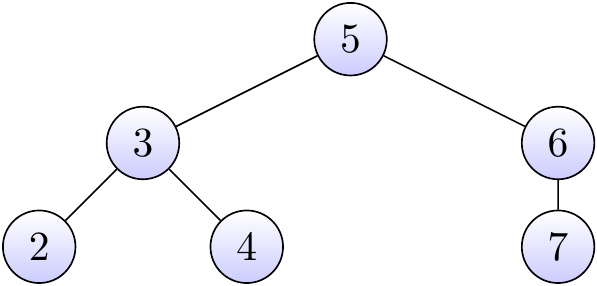
\includegraphics[width=0.9\linewidth]{tech-interview_files/figure-latex/unnamed-chunk-1-1} \caption{Some caption.}\label{fig:unnamed-chunk-1}
\end{figure}

Target = 9, Output = True.

\hypertarget{solution-2}{%
\subsection{Solution}\label{solution-2}}

\hypertarget{walkthrough-4}{%
\subsubsection{Walkthrough}\label{walkthrough-4}}

Use a HashSet to store value of current node, that is (node.val). Then check if answer = (target - node.val)
and return true if existed; otherwise, recursively call the same function for its left and right children.

\hypertarget{analysis-4}{%
\subsubsection{Analysis}\label{analysis-4}}

Time complexity is O(n) since every node is visited. Auxiliary Space is O(1)

\hypertarget{algorithm-4}{%
\subsubsection{Algorithm}\label{algorithm-4}}

recursion \ref{recursion}

\hypertarget{java-code-2}{%
\subsection{Java Code}\label{java-code-2}}

\begin{Shaded}
\begin{Highlighting}[]
\KeywordTok{public} \DataTypeTok{boolean} \FunctionTok{findTarget}\NormalTok{(}\BuiltInTok{TreeNode}\NormalTok{ root, }\DataTypeTok{int}\NormalTok{ target) \{}
    \BuiltInTok{Set}\NormalTok{<}\BuiltInTok{Integer}\NormalTok{> set = }\KeywordTok{new} \BuiltInTok{HashSet}\NormalTok{<>();}
    \KeywordTok{return} \FunctionTok{findTarget}\NormalTok{(root, target, set);}
\NormalTok{\}}

\KeywordTok{public} \DataTypeTok{boolean} \FunctionTok{findTarget}\NormalTok{(}\BuiltInTok{TreeNode}\NormalTok{ node, }\DataTypeTok{int}\NormalTok{ target, }\BuiltInTok{Set}\NormalTok{<}\BuiltInTok{Integer}\NormalTok{> set) \{}
    \KeywordTok{if}\NormalTok{(node == }\KeywordTok{null}\NormalTok{) \{}
        \KeywordTok{return} \KeywordTok{false}\NormalTok{;}
\NormalTok{    \} }\KeywordTok{else} \KeywordTok{if}\NormalTok{(set.}\FunctionTok{contains}\NormalTok{(target - node.}\FunctionTok{val}\NormalTok{)) \{}
        \KeywordTok{return} \KeywordTok{true}\NormalTok{;}
\NormalTok{    \} }\KeywordTok{else}\NormalTok{ \{}
        \CommentTok{//recursively calling}
\NormalTok{        set.}\FunctionTok{add}\NormalTok{(node.}\FunctionTok{val}\NormalTok{);}
        \KeywordTok{return} \FunctionTok{findTarget}\NormalTok{(node.}\FunctionTok{right}\NormalTok{, target, set) || }\FunctionTok{findTarget}\NormalTok{(node.}\FunctionTok{left}\NormalTok{, target, set);}
\NormalTok{    \}}

\NormalTok{\}}
\end{Highlighting}
\end{Shaded}

\hypertarget{twosum-v}{%
\section{TwoSum V / / \}}\label{twosum-v}}

\hypertarget{description-4}{%
\subsection{Description}\label{description-4}}

Given a sorted array S of n integers, are there elements a, b in S such that a + b = target? Find all unique
pairs in the array which gives the sum of zero. Note: The solution set must not contain duplicate triplets.

\hypertarget{example-3}{%
\subsection{Example}\label{example-3}}

For example, given array S = {[}-2, -1, -1, 0, 1, 2{]}, target = 0
A solution set is:
{[}
{[}-1, 1{]},
{[}-2, 2{]}{]}

\hypertarget{solution-3}{%
\subsection{Solution}\label{solution-3}}

\hypertarget{walkthrough-5}{%
\subsubsection{Walkthrough}\label{walkthrough-5}}

While searching for the other two elements from both ends, with indices left incrementally and right decrmentally, find
the sum = nums{[}left{]} + nums{[}right{]} == target. Since the array is
sorted, we need to avoid duplicated entry by moving forward the index while searching.

\hypertarget{analysis-5}{%
\subsubsection{Analysis}\label{analysis-5}}

There are one loops, the time complexity is \(O(n)\), and Auxiliary Space is \(O(n)\) since one member of any pair is
uniquely determined by the other member. If the numbers are not distinct, the Auxiliary Space as large as
\(O(\binom{n}{2}) = O(\frac{n!}{2!\cdot (n-2)!}) = O(\frac{n\cdot (n-1)}{2}) = O(n^2)\)

\hypertarget{algorithm-5}{%
\subsubsection{Algorithm}\label{algorithm-5}}

\hypertarget{java-code-3}{%
\subsection{Java Code}\label{java-code-3}}

\begin{Shaded}
\begin{Highlighting}[]
\KeywordTok{public} \BuiltInTok{List}\NormalTok{<}\BuiltInTok{List}\NormalTok{<}\BuiltInTok{Integer}\NormalTok{>> }\FunctionTok{twoSum}\NormalTok{(}\DataTypeTok{int}\NormalTok{[] num, }\DataTypeTok{int}\NormalTok{ target) \{}
    \BuiltInTok{List}\NormalTok{<}\BuiltInTok{List}\NormalTok{<}\BuiltInTok{Integer}\NormalTok{>> result = }\KeywordTok{new} \BuiltInTok{ArrayList}\NormalTok{<>();}

    \DataTypeTok{int}\NormalTok{ left = }\DecValTok{0}\NormalTok{, right = num.}\FunctionTok{length}\NormalTok{ - }\DecValTok{1}\NormalTok{;}

    \KeywordTok{while}\NormalTok{ (left < right) \{}
        \DataTypeTok{int}\NormalTok{ sum = num[left] + num[right];}

        \KeywordTok{if}\NormalTok{ (sum == target) \{}
\NormalTok{            result.}\FunctionTok{add}\NormalTok{(}\BuiltInTok{Arrays}\NormalTok{.}\FunctionTok{asList}\NormalTok{(num[left], num[right]));}

            \CommentTok{//avoid duplicated entry by moving forward the index}
            \KeywordTok{while}\NormalTok{ (left < right && num[left] == num[left + }\DecValTok{1}\NormalTok{]) \{}
\NormalTok{                left++;}
\NormalTok{            \}}
            \KeywordTok{while}\NormalTok{ (left < right && num[right] == num[right - }\DecValTok{1}\NormalTok{]) \{}
\NormalTok{                right--;}
\NormalTok{            \}}

\NormalTok{            left++;}
\NormalTok{            right--;}
\NormalTok{        \} }\KeywordTok{else} \KeywordTok{if}\NormalTok{ (sum < target) \{}
\NormalTok{            left++;}
\NormalTok{        \} }\KeywordTok{else}\NormalTok{ \{}
            \CommentTok{// sum > target}
\NormalTok{            right--;}
\NormalTok{        \}}
\NormalTok{    \}}

    \KeywordTok{return}\NormalTok{ result;}
\NormalTok{\}}
\end{Highlighting}
\end{Shaded}

\hypertarget{sum-leet-code-15-medium}{%
\section{3Sum / Leet Code 15 / Medium\}}\label{sum-leet-code-15-medium}}

\hypertarget{description-5}{%
\subsection{Description}\label{description-5}}

Given an array S of n integers, are there elements a, b, c in S such that a + b + c = 0? Find all unique triplets in the array which
gives the sum of zero. Note: The solution set must not contain duplicate triplets.

\hypertarget{example-4}{%
\subsection{Example}\label{example-4}}

For example, given array S = {[}-1, 0, 1, 2, -1, -4{]},
A solution set is:
{[}
{[}-1, 0, 1{]},
{[}-1, -1, 2{]}{]}

\hypertarget{solution-4}{%
\subsection{Solution}\label{solution-4}}

\hypertarget{walkthrough-6}{%
\subsubsection{Walkthrough}\label{walkthrough-6}}

Looping the array with index i, while searching for the other two elements from both ends, with indices
left incrementally and right decrmentally, find the sum = nums{[}i{]} + nums{[}left{]} + nums{[}right{]} == 0. Since the array is
sorted, we need to avoid duplicated entry by moving forward the index while searching.

\hypertarget{analysis-6}{%
\subsubsection{Analysis}\label{analysis-6}}

There are two nested loops, the time complexity is \(O(n^2)\), and Auxiliary Space is is \(O(n^2)\) since one member of any
triplet is uniquely determined by the other two members. If the numbers are not distinct, the Auxiliary Space as large as
\(O(\binom{n}{3}) = O(\frac{n!}{3!\cdot (n-3)!}) = O(\frac{n\cdot (n-1)\cdot(n-2)}{3}) = O(n^3)\)

\hypertarget{algorithm-6}{%
\subsubsection{Algorithm}\label{algorithm-6}}

\hypertarget{java-code-4}{%
\subsection{Java Code}\label{java-code-4}}

\begin{Shaded}
\begin{Highlighting}[]
\KeywordTok{public} \BuiltInTok{List}\NormalTok{<}\BuiltInTok{List}\NormalTok{<}\BuiltInTok{Integer}\NormalTok{>> }\FunctionTok{threeSum}\NormalTok{(}\DataTypeTok{int}\NormalTok{[] num) \{}
    \BuiltInTok{Arrays}\NormalTok{.}\FunctionTok{sort}\NormalTok{(num); }\CommentTok{//sort}
    \BuiltInTok{List}\NormalTok{<}\BuiltInTok{List}\NormalTok{<}\BuiltInTok{Integer}\NormalTok{>> result = }\KeywordTok{new} \BuiltInTok{ArrayList}\NormalTok{<>();}

    \CommentTok{//last possible pair is [i=len - 3, left=len - 2, right=len - 1]}
    \KeywordTok{for}\NormalTok{ (}\DataTypeTok{int}\NormalTok{ i = }\DecValTok{0}\NormalTok{; i < num.}\FunctionTok{length}\NormalTok{ - }\DecValTok{2}\NormalTok{; i++) \{}
        \CommentTok{// Since the array is sorted, we need to avoid duplicated entry by moving forward the index}
        \KeywordTok{if}\NormalTok{ (i == }\DecValTok{0}\NormalTok{ || (i > }\DecValTok{0}\NormalTok{ && num[i] != num[i}\DecValTok{-1}\NormalTok{])) \{}
            \DataTypeTok{int}\NormalTok{ left = i + }\DecValTok{1}\NormalTok{, right = num.}\FunctionTok{length}\DecValTok{-1}\NormalTok{;}

            \KeywordTok{while}\NormalTok{ (left < right) \{}
                \DataTypeTok{int}\NormalTok{ sum = num[i] + num[left] + num[right];}

                \KeywordTok{if}\NormalTok{ (sum == }\DecValTok{0}\NormalTok{) \{}
\NormalTok{                    result.}\FunctionTok{add}\NormalTok{(}\BuiltInTok{Arrays}\NormalTok{.}\FunctionTok{asList}\NormalTok{(num[i], num[left], num[right]));}

                    \CommentTok{//avoid duplicated entry by moving forward the index}
                    \KeywordTok{while}\NormalTok{ (left < right && num[left] == num[left + }\DecValTok{1}\NormalTok{]) \{}
\NormalTok{                        left++;}
\NormalTok{                    \}}
                    \KeywordTok{while}\NormalTok{ (left < right && num[right] == num[right - }\DecValTok{1}\NormalTok{]) \{}
\NormalTok{                        right--;}
\NormalTok{                    \}}

\NormalTok{                    left++;}
\NormalTok{                    right--;}
\NormalTok{                \} }\KeywordTok{else} \KeywordTok{if}\NormalTok{ (sum < }\DecValTok{0}\NormalTok{) \{}
\NormalTok{                    left++;}
\NormalTok{                \} }\KeywordTok{else}\NormalTok{ \{}
                    \CommentTok{// sum > 0}
\NormalTok{                    right--;}
\NormalTok{                \}}
\NormalTok{            \}}
\NormalTok{        \}}
\NormalTok{    \}}

    \KeywordTok{return}\NormalTok{ result;}
\NormalTok{\}}
\end{Highlighting}
\end{Shaded}

\hypertarget{sum-closest-leetcode-16-medium}{%
\section{3 Sum Closest / LeetCode 16 / Medium\}}\label{sum-closest-leetcode-16-medium}}

\hypertarget{description-6}{%
\subsection{Description}\label{description-6}}

Given an array S of n integers, find three integers in S such that the sum is closest to a given number, target.
Return the sum of the three integers. You may assume that each input would have exactly one solution.

\hypertarget{example-5}{%
\subsection{Example}\label{example-5}}

For example, given array S = -1 2 1 -4, and target = 1.
The sum that is closest to the target is 2. (-1 + 2 + 1 = 2).

\hypertarget{solution-5}{%
\subsection{Solution}\label{solution-5}}

\hypertarget{walkthrough-7}{%
\subsubsection{Walkthrough}\label{walkthrough-7}}

Looping the array with index i, while searching for the other two elements from both ends, with indices
left incrementally and right decrmentally, find the sum = nums{[}i{]} + nums{[}left{]} + nums{[}right{]}. Return sum if existed;
otherwise, keep for the closest tuple of (nums{[}i{]}, nums{[}left{]}, nums{[}right{]}) against target using Math.abs().

\hypertarget{analysis-7}{%
\subsubsection{Analysis}\label{analysis-7}}

There are two nested loops, the time complexity is \(O(n^2)\), and Auxiliary Space is O(1) since it is returning the closest answer.

\hypertarget{algorithm-7}{%
\subsubsection{Algorithm}\label{algorithm-7}}

\hypertarget{java-code-5}{%
\subsection{Java Code}\label{java-code-5}}

\begin{Shaded}
\begin{Highlighting}[]
\KeywordTok{public} \DataTypeTok{int} \FunctionTok{threeSumClosest}\NormalTok{(}\DataTypeTok{int}\NormalTok{[] nums, }\DataTypeTok{int}\NormalTok{ target) \{}
    \BuiltInTok{Arrays}\NormalTok{.}\FunctionTok{sort}\NormalTok{(num); }\CommentTok{//sort}
    \DataTypeTok{int}\NormalTok{ minDelta = }\BuiltInTok{Integer}\NormalTok{.}\FunctionTok{MAX_VALUE}\NormalTok{, result = }\DecValTok{0}\NormalTok{;}

    \CommentTok{//last possible pair is [i=len - 3, left=len - 2, right=len - 1]}
    \KeywordTok{for}\NormalTok{ (}\DataTypeTok{int}\NormalTok{ i = }\DecValTok{0}\NormalTok{; i < num.}\FunctionTok{length}\NormalTok{ - }\DecValTok{2}\NormalTok{; i++) \{}
        \DataTypeTok{int}\NormalTok{ left = i + }\DecValTok{1}\NormalTok{, right = num.}\FunctionTok{length}\NormalTok{ - }\DecValTok{1}\NormalTok{;}

        \KeywordTok{while}\NormalTok{ (left < right) \{}
            \DataTypeTok{int}\NormalTok{ sum = num[i] + num[left] + num[right];}

            \KeywordTok{if}\NormalTok{ (sum == target) \{}
                \CommentTok{//find exact match}
                \KeywordTok{return}\NormalTok{ sum;}
\NormalTok{            \} }\KeywordTok{else} \KeywordTok{if}\NormalTok{ (sum < target) \{}
\NormalTok{                left++;}
\NormalTok{            \} }\KeywordTok{else}\NormalTok{ \{}
                \CommentTok{// sum > target}
\NormalTok{                right--;}
\NormalTok{            \}}

            \DataTypeTok{int}\NormalTok{ delta = }\BuiltInTok{Math}\NormalTok{.}\FunctionTok{abs}\NormalTok{(sum - target);}
            \KeywordTok{if}\NormalTok{(delta < minDelta) \{}
\NormalTok{                minDelta = delta;}
\NormalTok{                result = sum;}
\NormalTok{            \}}
\NormalTok{        \}}
\NormalTok{    \}}

    \KeywordTok{return}\NormalTok{ result;}
\NormalTok{\}}
\end{Highlighting}
\end{Shaded}

\hypertarget{sum-leet-code-18-medium}{%
\section{4Sum / Leet Code 18 / Medium\}}\label{sum-leet-code-18-medium}}

\hypertarget{description-7}{%
\subsection{Description}\label{description-7}}

Given an array nums of n integers and an integer target, are there elements a, b, c, and d in nums such that
a + b + c + d = target? Find all unique quadruplets in the array which gives the sum of target. The solution set
must not contain duplicate quadruplets.

\hypertarget{example-6}{%
\subsection{Example}\label{example-6}}

Given array nums = {[}1, 0, -1, 0, -2, 2{]}, and target = 0.

A solution set is:
{[}
{[}-1, 0, 0, 1{]},
{[}-2, -1, 1, 2{]},
{[}-2, 0, 0, 2{]}{]}

\hypertarget{solution-6}{%
\subsection{Solution}\label{solution-6}}

\hypertarget{walkthrough-8}{%
\subsubsection{Walkthrough}\label{walkthrough-8}}

The solution is similar to 3Sum to find the sum = nums{[}i{]} + nums{[}j{]} + nums{[}left{]} + nums{[}right{]} == target. The only
difference is there is an extra loop as well as we need to avoid duplicated entry by moving forward the index
during search.

\hypertarget{analysis-8}{%
\subsubsection{Analysis}\label{analysis-8}}

Overall, there are three nested loops, the time complexity is \(O(n^3)\), and Auxiliary Space is \(O(n^3)\) since one member
of any quotriplet is uniquely determined by the other three member. If the numbers are not distinct, the Auxiliary
Space as large as is \(O(\binom{n}{4}) = O(n^4)\)

\hypertarget{algorithm-8}{%
\subsubsection{Algorithm}\label{algorithm-8}}

\hypertarget{java-code-6}{%
\subsection{Java Code}\label{java-code-6}}

\begin{Shaded}
\begin{Highlighting}[]
\KeywordTok{public} \BuiltInTok{List}\NormalTok{<}\BuiltInTok{List}\NormalTok{<}\BuiltInTok{Integer}\NormalTok{>> }\FunctionTok{fourSum}\NormalTok{(}\DataTypeTok{int}\NormalTok{[] num, }\DataTypeTok{int}\NormalTok{ target) \{}
    \BuiltInTok{Arrays}\NormalTok{.}\FunctionTok{sort}\NormalTok{(num); }\CommentTok{//sort}
    \BuiltInTok{List}\NormalTok{<}\BuiltInTok{List}\NormalTok{<}\BuiltInTok{Integer}\NormalTok{>> res = }\KeywordTok{new} \BuiltInTok{LinkedList}\NormalTok{<>();}

    \CommentTok{//last possible pair is [j=len - 4, i=len-3, left=len - 2, right=len - 1]}
    \KeywordTok{for}\NormalTok{ (}\DataTypeTok{int}\NormalTok{ j = }\DecValTok{0}\NormalTok{; i < num.}\FunctionTok{length}\NormalTok{ - }\DecValTok{3}\NormalTok{; i++) \{}

        \CommentTok{// Since the array is sorted, we need to avoid duplicated entry by moving forward the index}
        \KeywordTok{if}\NormalTok{ (j == }\DecValTok{0}\NormalTok{ || (j > }\DecValTok{0}\NormalTok{ && num[j] != num[j - }\DecValTok{1}\NormalTok{])) \{}
            \KeywordTok{for}\NormalTok{ (}\DataTypeTok{int}\NormalTok{ i = j + }\DecValTok{1}\NormalTok{; i < num.}\FunctionTok{length}\NormalTok{ - }\DecValTok{2}\NormalTok{; i++) \{}

                \CommentTok{// Since the array is sorted, we need to avoid duplicated entry by moving forward the index}
                \KeywordTok{if}\NormalTok{ (i == j + }\DecValTok{1}\NormalTok{ || (i > }\DecValTok{0}\NormalTok{ && num[i] != num[i - }\DecValTok{1}\NormalTok{])) \{}
                    \DataTypeTok{int}\NormalTok{ left = i + }\DecValTok{1}\NormalTok{, right = num.}\FunctionTok{length}\DecValTok{-1}\NormalTok{;}

                    \KeywordTok{while}\NormalTok{ (left < right) \{}
                        \DataTypeTok{int}\NormalTok{ sum = num[i] + num[j] + num[left] + num[right];}

                        \KeywordTok{if}\NormalTok{ (sum == target) \{}
\NormalTok{                            res.}\FunctionTok{add}\NormalTok{(}\BuiltInTok{Arrays}\NormalTok{.}\FunctionTok{asList}\NormalTok{(num[i], num[j], num[left], num[right]));}

                            \CommentTok{//avoid duplicated entry by moving forward the index}
                            \KeywordTok{while}\NormalTok{ (left < right && num[left] == num[left + }\DecValTok{1}\NormalTok{]) \{}
\NormalTok{                                left++;}
\NormalTok{                            \}}
                            \KeywordTok{while}\NormalTok{ (left < right && num[right] == num[right - }\DecValTok{1}\NormalTok{]) \{}
\NormalTok{                                right--;}
\NormalTok{                            \}}
\NormalTok{                            left++;}
\NormalTok{                            right--;}
\NormalTok{                        \} }\KeywordTok{else} \KeywordTok{if}\NormalTok{ (sum < target) \{}
\NormalTok{                            left++;}
\NormalTok{                        \} }\KeywordTok{else}\NormalTok{ \{}
                            \CommentTok{// sum > 0}
\NormalTok{                            right--;}
\NormalTok{                        \}}
\NormalTok{                    \}}
\NormalTok{                \}}
\NormalTok{            \}}
\NormalTok{        \}}
\NormalTok{    \}}

    \KeywordTok{return}\NormalTok{ res;}
\NormalTok{\}}
\end{Highlighting}
\end{Shaded}

\hypertarget{sum-ii}{%
\section{4Sum II\}}\label{sum-ii}}

\hypertarget{description-8}{%
\subsection{Description}\label{description-8}}

Given four lists A, B, C, D of integer values, compute how many tuples (i, j, k, l) there are such that
A{[}i{]} + B{[}j{]} + C{[}k{]} + D{[}l{]} is zero.

To make problem a bit easier, all A, B, C, D have same length of N where \(0 \le N \le 500\). All integers are
in the range of \(-2^{28}\) to \(2^{28} - 1\) and the result is guaranteed to be at most \(2^{31} - 1\).

\hypertarget{example-7}{%
\subsection{Example}\label{example-7}}

Input:
A = {[} 1, 2{]}
B = {[}-2,-1{]}
C = {[}-1, 2{]}
D = {[} 0, 2{]}

Output:
2

Explanation:
The two tuples are:
1. (0, 0, 0, 1) \(->\) A{[}0{]} + B{[}0{]} + C{[}0{]} + D{[}1{]} = 1 + (-2) + (-1) + 2 = 0
2. (1, 1, 0, 0) \(->\) A{[}1{]} + B{[}1{]} + C{[}0{]} + D{[}0{]} = 2 + (-1) + (-1) + 0 = 0
\#\#\# Solution
\#\#\#\# Walkthrough
*Rewrite the equation as A{[}i{]} + B{[}j{]} = -(C{[}k{]} + D{[}l{]}).
Create a Map\textless{}Integer, Integer\textgreater{} where `key' is A{[}i{]} + B{[}j{]} and `value' is the number of pairs with this sum.
For each -(C{[}k{]} + D{[}l{]}), see if this desired sum is in our map. If so, add the map's `value' to our total count.

\hypertarget{analysis-9}{%
\subsubsection{Analysis}\label{analysis-9}}

There are two nested loops, the time complexity is \(O(n^2)\), and Auxiliary Space for Map is O(n)

\hypertarget{algorithm-9}{%
\subsubsection{Algorithm}\label{algorithm-9}}

\hypertarget{java-code-7}{%
\subsection{Java Code}\label{java-code-7}}

\begin{Shaded}
\begin{Highlighting}[]
\KeywordTok{public} \DataTypeTok{int} \FunctionTok{fourSumCount}\NormalTok{(}\DataTypeTok{int}\NormalTok{[] A, }\DataTypeTok{int}\NormalTok{[] B, }\DataTypeTok{int}\NormalTok{[] C, }\DataTypeTok{int}\NormalTok{[] D) \{}
    \DataTypeTok{int}\NormalTok{ n = A.}\FunctionTok{length}\NormalTok{;}

    \KeywordTok{if}\NormalTok{(n == }\DecValTok{0}\NormalTok{) \{}
        \KeywordTok{return} \DecValTok{0}\NormalTok{;}
\NormalTok{    \}}

    \DataTypeTok{int}\NormalTok{[] sumOfAandB = }\KeywordTok{new} \DataTypeTok{int}\NormalTok{[n * n];}
    \DataTypeTok{int}\NormalTok{ result = }\DecValTok{0}\NormalTok{;}

    \BuiltInTok{HashMap}\NormalTok{<}\BuiltInTok{Integer}\NormalTok{, }\BuiltInTok{Integer}\NormalTok{> map = }\KeywordTok{new} \BuiltInTok{HashMap}\NormalTok{<}\BuiltInTok{Integer}\NormalTok{, }\BuiltInTok{Integer}\NormalTok{>();}

    \KeywordTok{for}\NormalTok{(}\DataTypeTok{int}\NormalTok{ i = }\DecValTok{0}\NormalTok{; i < n; i++)\{}
        \KeywordTok{for}\NormalTok{(}\DataTypeTok{int}\NormalTok{ j = }\DecValTok{0}\NormalTok{; j < n; j++)\{}
\NormalTok{            sumOfAandB[i*n + j] = A[i] + B[j];}

            \CommentTok{//record # of pairs for this sum of [A, B]}
            \DataTypeTok{int}\NormalTok{ count = map.}\FunctionTok{getOrDefault}\NormalTok{(sumOfAandB[i*n + j], }\DecValTok{0}\NormalTok{) + }\DecValTok{1}\NormalTok{;}
\NormalTok{            map.}\FunctionTok{put}\NormalTok{(sumOfAandB[i*n + j], count);}
\NormalTok{        \}}
\NormalTok{    \}}

    \CommentTok{//A + B = - (C + D)}
    \KeywordTok{for}\NormalTok{(}\DataTypeTok{int}\NormalTok{ i = }\DecValTok{0}\NormalTok{; i < n; i++)\{}
        \KeywordTok{for}\NormalTok{(}\DataTypeTok{int}\NormalTok{ j = }\DecValTok{0}\NormalTok{; j < n; j++)\{}
            \DataTypeTok{int}\NormalTok{ sumOfCandD = - (C[i] + D[j]);}

            \KeywordTok{if}\NormalTok{(map.}\FunctionTok{containsKey}\NormalTok{(sumOfCandD))\{}
\NormalTok{                result += map.}\FunctionTok{get}\NormalTok{(sumOfCandD);}
\NormalTok{            \}}
\NormalTok{        \}}
\NormalTok{    \}}


    \KeywordTok{return}\NormalTok{ result;}
\NormalTok{\}}
\end{Highlighting}
\end{Shaded}

\hypertarget{max-gain-firecode-level-2}{%
\section{Max Gain / Firecode / Level 2\}}\label{max-gain-firecode-level-2}}

\hypertarget{description-9}{%
\subsection{Description}\label{description-9}}

Given an array of integers, write a method - maxGain - that returns the maximum gain. Maximum Gain is defined as the
maximum difference between 2 elements in a list such that the larger element appears after the smaller element. If no
gain is possible, return 0.

\hypertarget{example-8}{%
\subsection{Example}\label{example-8}}

{[}0,50,10,100,30{]} returns 100

{[}100,40,20,10{]} returns 0

{[}0,100,0,100,0,100{]} returns 100

\hypertarget{solution-7}{%
\subsection{Solution}\label{solution-7}}

\hypertarget{walkthrough-9}{%
\subsubsection{Walkthrough}\label{walkthrough-9}}

By definition, \textbf{the larger element must always appear after the smaller element}, we could do this in one pass
by finding the minimum element and the maximum gain (so far) by Math.max(min, a{[}i{]} - min)

\hypertarget{analysis-10}{%
\subsubsection{Analysis}\label{analysis-10}}

The time complexity is O(n) since every element is visited in the loop.

\hypertarget{algorithm-10}{%
\subsubsection{Algorithm}\label{algorithm-10}}

\hypertarget{java-code-8}{%
\subsection{Java Code}\label{java-code-8}}

\begin{Shaded}
\begin{Highlighting}[]
\KeywordTok{public} \DataTypeTok{static} \DataTypeTok{int} \FunctionTok{maxGain}\NormalTok{(}\DataTypeTok{int}\NormalTok{[] a) \{}
    \DataTypeTok{int}\NormalTok{ min = }\BuiltInTok{Integer}\NormalTok{.}\FunctionTok{MAX_VALUE}\NormalTok{, gain = }\DecValTok{0}\NormalTok{;}

    \KeywordTok{for}\NormalTok{(}\DataTypeTok{int}\NormalTok{ i = }\DecValTok{0}\NormalTok{; i < a.}\FunctionTok{length}\NormalTok{; i++) \{}
\NormalTok{        min = }\BuiltInTok{Math}\NormalTok{.}\FunctionTok{min}\NormalTok{(min, a[i]);}
\NormalTok{        gain = }\BuiltInTok{Math}\NormalTok{.}\FunctionTok{max}\NormalTok{(gain, a[i] - min);}
\NormalTok{    \}}

    \KeywordTok{return}\NormalTok{ gain;}
\NormalTok{\}}
\end{Highlighting}
\end{Shaded}

\hypertarget{pascals-triangle-leet-code-118-easy}{%
\section{Pascal's Triangle / Leet Code 118 / Easy\}}\label{pascals-triangle-leet-code-118-easy}}

\hypertarget{description-10}{%
\subsection{Description}\label{description-10}}

Given a non-negative integer numRows, generate the first numRows of Pascal's triangle. In Pascal's triangle, each
number is the sum of the two numbers directly above it.

\hypertarget{example-9}{%
\subsection{Example}\label{example-9}}

\hypertarget{solution-8}{%
\subsection{Solution}\label{solution-8}}

\hypertarget{walkthrough-10}{%
\subsubsection{Walkthrough}\label{walkthrough-10}}

For level 1 and level 2, add number 1. For level 3 or above if it is the first or last element, insert 1, otherwise,
insert the sum of last two elements in the level above : {[}i-1{]}{[}j{]} + {[}i-1{]}{[}j-1{]}.

\hypertarget{analysis-11}{%
\subsubsection{Analysis}\label{analysis-11}}

There are two nested loops, the time complexity is \(O(n^2)\)\$, and Auxiliary Space is \(O(n^2)\).

\hypertarget{algorithm-11}{%
\subsubsection{Algorithm}\label{algorithm-11}}

\hypertarget{java-code-9}{%
\subsection{Java Code}\label{java-code-9}}

\begin{Shaded}
\begin{Highlighting}[]
\KeywordTok{public} \BuiltInTok{List}\NormalTok{<}\BuiltInTok{List}\NormalTok{<}\BuiltInTok{Integer}\NormalTok{>> }\FunctionTok{generate}\NormalTok{(}\DataTypeTok{int}\NormalTok{ numRows) \{}
    \BuiltInTok{List}\NormalTok{<}\BuiltInTok{List}\NormalTok{<}\BuiltInTok{Integer}\NormalTok{>> triangle = }\KeywordTok{new} \BuiltInTok{ArrayList}\NormalTok{<>();}

    \KeywordTok{for}\NormalTok{(}\DataTypeTok{int}\NormalTok{ i = }\DecValTok{0}\NormalTok{; i < numRows; i++) \{}
        \BuiltInTok{List}\NormalTok{<}\BuiltInTok{Integer}\NormalTok{> level = }\KeywordTok{new} \BuiltInTok{ArrayList}\NormalTok{<>();}

        \KeywordTok{for}\NormalTok{(}\DataTypeTok{int}\NormalTok{ j = }\DecValTok{0}\NormalTok{; j < (i+}\DecValTok{1}\NormalTok{); j++) \{}
            \KeywordTok{if}\NormalTok{(i == }\DecValTok{0}\NormalTok{ || i == }\DecValTok{1}\NormalTok{) \{}
                \CommentTok{// for level 1 or level 2}
\NormalTok{                level.}\FunctionTok{add}\NormalTok{(}\DecValTok{1}\NormalTok{);}
\NormalTok{            \} }\KeywordTok{else}\NormalTok{ \{}
                \CommentTok{// for level 3 or above}
                \KeywordTok{if}\NormalTok{(j == }\DecValTok{0}\NormalTok{ || j == i) \{}
\NormalTok{                    level.}\FunctionTok{add}\NormalTok{(}\DecValTok{1}\NormalTok{);}
\NormalTok{                \} }\KeywordTok{else}\NormalTok{ \{}
                    \DataTypeTok{int}\NormalTok{ op1 = triangle.}\FunctionTok{get}\NormalTok{(i}\DecValTok{-1}\NormalTok{).}\FunctionTok{get}\NormalTok{(j}\DecValTok{-1}\NormalTok{);}
                    \DataTypeTok{int}\NormalTok{ op2 = triangle.}\FunctionTok{get}\NormalTok{(i}\DecValTok{-1}\NormalTok{).}\FunctionTok{get}\NormalTok{(j);}
\NormalTok{                    level.}\FunctionTok{add}\NormalTok{(op1 + op2);}
\NormalTok{                \}}
\NormalTok{            \}}
\NormalTok{        \}}

\NormalTok{        triangle.}\FunctionTok{add}\NormalTok{(level);}
\NormalTok{    \}}

    \KeywordTok{return}\NormalTok{ triangle;}
\NormalTok{\}}
\end{Highlighting}
\end{Shaded}

\hypertarget{search-in-rotated-sorted-array-leet-code-33-medium}{%
\section{Search in Rotated Sorted Array / Leet Code 33 / Medium \}}\label{search-in-rotated-sorted-array-leet-code-33-medium}}

\hypertarget{description-11}{%
\subsection{Description}\label{description-11}}

Suppose an array sorted in ascending order is rotated at some pivot unknown to you beforehand.
(i.e., {[}0,1,2,4,5,6,7{]} might become {[}4,5,6,7,0,1,2{]}).

You are given a target value to search. If found in the array return its index, otherwise return -1. You may
assume no duplicate exists in the array. Your algorithm's runtime complexity must be in the order of O(log n).

\hypertarget{example-10}{%
\subsection{Example}\label{example-10}}

Input: nums = {[}4,5,6,7,0,1,2{]}, target = 0
Output: 4

Input: nums = {[}4,5,6,7,0,1,2{]}, target = 3
Output: -1
\#\#\# Solution
\#\#\#\# Walkthrough
The key point is to search the element in a divide-and-conquer manner. We need to repeated compare the
mid element of index = (left + right) / 2 with target and keep shrinking the boundaries from left and right two ends
according to the conditions. Return the mid index if found; otherwise, return -1.

\hypertarget{analysis-12}{%
\subsubsection{Analysis}\label{analysis-12}}

The time complexity is O(log n) since we only pick one from half of target elements each time.

\hypertarget{algorithm-12}{%
\subsubsection{Algorithm}\label{algorithm-12}}

dnc \ref{dnc}

\hypertarget{java-code-10}{%
\subsection{Java Code}\label{java-code-10}}

\begin{Shaded}
\begin{Highlighting}[]
\KeywordTok{public} \DataTypeTok{int} \FunctionTok{search}\NormalTok{(}\DataTypeTok{int}\NormalTok{[] nums, }\DataTypeTok{int}\NormalTok{ target) \{}
    \DataTypeTok{int}\NormalTok{ left = }\DecValTok{0}\NormalTok{, right = nums.}\FunctionTok{length}\NormalTok{ - }\DecValTok{1}\NormalTok{;}

    \KeywordTok{while}\NormalTok{(left <= right) \{}
        \DataTypeTok{int}\NormalTok{ mid = (right - left) / }\DecValTok{2}\NormalTok{ + left;}

        \KeywordTok{if}\NormalTok{(nums[mid] == target) \{}
            \CommentTok{//Found index}
            \KeywordTok{return}\NormalTok{ mid;}
\NormalTok{        \} }\KeywordTok{else} \KeywordTok{if}\NormalTok{(nums[mid] >= nums[left]) \{}
            \CommentTok{//left half of array}
            \KeywordTok{if}\NormalTok{(target >= nums[left] && target < nums[mid]) \{}
                \CommentTok{//<-- moving leftward}
\NormalTok{                right = mid }\DecValTok{-1}\NormalTok{;}
\NormalTok{            \} }\KeywordTok{else}\NormalTok{ \{}
                \CommentTok{//--> moving rightward}
\NormalTok{                left = mid + }\DecValTok{1}\NormalTok{;}
\NormalTok{            \}}
\NormalTok{        \} }\KeywordTok{else}\NormalTok{ \{}
            \CommentTok{//nums[mid] < nums[right}
            \CommentTok{//right half of array}
            \KeywordTok{if}\NormalTok{(target > nums[mid] && target <= nums[right]) \{}
                \CommentTok{//--> moving rightward}
\NormalTok{                left = mid + }\DecValTok{1}\NormalTok{;}
\NormalTok{            \} }\KeywordTok{else}\NormalTok{ \{}
                \CommentTok{//<-- moving leftward}
\NormalTok{                right = mid - }\DecValTok{1}\NormalTok{;}
\NormalTok{            \}}
\NormalTok{        \}}
\NormalTok{    \}}

    \KeywordTok{return} \DecValTok{-1}\NormalTok{;}
\NormalTok{\}}
\end{Highlighting}
\end{Shaded}

\hypertarget{median-of-two-sorted-arrays-leet-code-4-hard}{%
\section{Median of Two Sorted Arrays / Leet Code 4 / Hard\}}\label{median-of-two-sorted-arrays-leet-code-4-hard}}

\hypertarget{description-12}{%
\subsection{Description}\label{description-12}}

There are two sorted arrays nums1 and nums2 of size m and n respectively. Find the median of the two sorted
arrays. The overall run time complexity should be O(log (m+n)). You may assume nums1 and nums2 cannot be both
empty.

\hypertarget{example-11}{%
\subsection{Example}\label{example-11}}

nums1 = {[}1, 3{]}, nums2 = {[}2{]}, The median is 2.0

nums1 = {[}1, 2{]}, nums2 = {[}3, 4{]}, The median is (2 + 3)/2 = 2.5

\hypertarget{solution-9}{%
\subsection{Solution}\label{solution-9}}

\hypertarget{walkthrough-11}{%
\subsubsection{Walkthrough}\label{walkthrough-11}}

Recursively find \(K^{th}\) element in two sorted array by comparing and discarding the \(\frac{k}{2}\) smaller
elements.

\hypertarget{analysis-13}{%
\subsubsection{Analysis}\label{analysis-13}}

For each round of recursive, it is eliminating \(\frac{k}{2}\) element, so total time complexity is
\(O(log(k)) = O(log(m + n))\). Auxiliary Space is O(1).

\hypertarget{algorithm-13}{%
\subsubsection{Algorithm}\label{algorithm-13}}

recursion \ref{recursion}

\hypertarget{java-code-11}{%
\subsection{Java Code}\label{java-code-11}}

\begin{Shaded}
\begin{Highlighting}[]
\KeywordTok{public} \DataTypeTok{double} \FunctionTok{findMedianSortedArrays}\NormalTok{(}\DataTypeTok{int}\NormalTok{[] nums1, }\DataTypeTok{int}\NormalTok{[] nums2) \{}
    \DataTypeTok{int}\NormalTok{ len1 = nums1.}\FunctionTok{length}\NormalTok{;}
    \DataTypeTok{int}\NormalTok{ len2 = nums2.}\FunctionTok{length}\NormalTok{;}
    \DataTypeTok{int}\NormalTok{ total = len1 + len2;}

    \KeywordTok{if}\NormalTok{ ((total & }\DecValTok{1}\NormalTok{) != }\DecValTok{0}\NormalTok{) \{}
        \CommentTok{// odd number length}
        \KeywordTok{return} \FunctionTok{findKth}\NormalTok{(nums1, }\DecValTok{0}\NormalTok{, len1 - }\DecValTok{1}\NormalTok{, nums2, }\DecValTok{0}\NormalTok{, len2 - }\DecValTok{1}\NormalTok{, total / }\DecValTok{2}\NormalTok{ + }\DecValTok{1}\NormalTok{);}
\NormalTok{    \} }\KeywordTok{else}\NormalTok{ \{}
        \CommentTok{// even number length}
        \KeywordTok{return}\NormalTok{ (}\FunctionTok{findKth}\NormalTok{(nums1, }\DecValTok{0}\NormalTok{, len1 - }\DecValTok{1}\NormalTok{, nums2, }\DecValTok{0}\NormalTok{, len2 - }\DecValTok{1}\NormalTok{, total / }\DecValTok{2}\NormalTok{) + }\FunctionTok{findKth}\NormalTok{(nums1, }\DecValTok{0}\NormalTok{, len1 - }\DecValTok{1}\NormalTok{, nums2, }\DecValTok{0}\NormalTok{, len2 - }\DecValTok{1}\NormalTok{, total / }\DecValTok{2}\NormalTok{ + }\DecValTok{1}\NormalTok{)) * }\FloatTok{0.5}\NormalTok{;}
\NormalTok{    \}}
\NormalTok{\}}

\KeywordTok{private} \DataTypeTok{int} \FunctionTok{findKth}\NormalTok{(}\DataTypeTok{int}\NormalTok{[] nums1, }\DataTypeTok{int}\NormalTok{ start1, }\DataTypeTok{int}\NormalTok{ end1, }\DataTypeTok{int}\NormalTok{[] nums2, }\DataTypeTok{int}\NormalTok{ start2, }\DataTypeTok{int}\NormalTok{ end2, }\DataTypeTok{int}\NormalTok{ k)\{}
    \DataTypeTok{int}\NormalTok{ len1 = end1 - start1 + }\DecValTok{1}\NormalTok{;}
    \DataTypeTok{int}\NormalTok{ len2 = end2 - start2 + }\DecValTok{1}\NormalTok{;}

    \CommentTok{/*}
\CommentTok{    * swap parameters for nums1 with nums2}
\CommentTok{    */}
    \KeywordTok{if}\NormalTok{ (len1 > len2) \{}
        \KeywordTok{return} \FunctionTok{findKth}\NormalTok{(nums2, start2, end2, nums1, start1, end1, k);}
\NormalTok{    \}}

    \KeywordTok{if}\NormalTok{ (len1 == }\DecValTok{0}\NormalTok{) \{}
        \KeywordTok{return}\NormalTok{ nums2[start2 + k - }\DecValTok{1}\NormalTok{];}
\NormalTok{    \}}

    \KeywordTok{if}\NormalTok{ (k == }\DecValTok{1}\NormalTok{) \{}
        \CommentTok{//return the smaller element of nums1[] and nums2[]}
        \KeywordTok{return} \BuiltInTok{Math}\NormalTok{.}\FunctionTok{min}\NormalTok{(nums1[start1], nums2[start2]);}
\NormalTok{    \}}

    \CommentTok{//Calculate number of elements to discard for next recursive}
    \DataTypeTok{int}\NormalTok{ endToDiscard1 = start1 + }\BuiltInTok{Math}\NormalTok{.}\FunctionTok{min}\NormalTok{(len1, k / }\DecValTok{2}\NormalTok{) - }\DecValTok{1}\NormalTok{;}
    \DataTypeTok{int}\NormalTok{ endToDiscard2 = start2 + }\BuiltInTok{Math}\NormalTok{.}\FunctionTok{min}\NormalTok{(len2, k / }\DecValTok{2}\NormalTok{) - }\DecValTok{1}\NormalTok{;}

    \KeywordTok{if}\NormalTok{ (nums1[endToDiscard1] > nums2[endToDiscard2]) \{}
        \CommentTok{//if nums2[] are smaller, discard, and start from following position recursively}
        \DataTypeTok{int}\NormalTok{ newK = k - (endToDiscard2 - start2 + }\DecValTok{1}\NormalTok{);}
        \KeywordTok{return} \FunctionTok{findKth}\NormalTok{(nums1, start1, end1, nums2, endToDiscard2 + }\DecValTok{1}\NormalTok{, end2, newK);}
\NormalTok{    \} }\KeywordTok{else}\NormalTok{ \{}
        \CommentTok{//if nums1[] are smaller, discard, and start from following position recursively}
        \DataTypeTok{int}\NormalTok{ newK = k - (endToDiscard1 - start1 + }\DecValTok{1}\NormalTok{);}
        \KeywordTok{return} \FunctionTok{findKth}\NormalTok{(nums1, endToDiscard1 + }\DecValTok{1}\NormalTok{, end1, nums2, start2, end2, newK);}
\NormalTok{    \}}
\NormalTok{\}}
\end{Highlighting}
\end{Shaded}

\hypertarget{retrieve-list-of-elements-appeared-at-kth-time-and-in-insertion-order}{%
\section{\texorpdfstring{Retrieve List of Elements Appeared at \(k^{th}\) Time and in Insertion Order / /\}}{Retrieve List of Elements Appeared at k\^{}\{th\} Time and in Insertion Order / /\}}}\label{retrieve-list-of-elements-appeared-at-kth-time-and-in-insertion-order}}

\hypertarget{description-13}{%
\subsection{Description}\label{description-13}}

Given an unsorted, possibly duplicated elments of array, return the list of element which appeared at kth
time where k \(>=\) 1. The returned elements need to be stable as they were in insertion order.

\hypertarget{example-12}{%
\subsection{Example}\label{example-12}}

\([1_1, 2_1, 3_1, 4_1, 2_2, 1_2, 1_3, 3_2], k = 1. => [1_1, 2_1, 3_1, 4_1]\)

\([1_1, 2_1, 3_1, 4_1, 2_2, 1_2, 1_3, 3_2], k = 2. => [2_2, 1_2, 3_2]\)

\([1_1, 2_1, 3_1, 4_1, 2_2, 1_2, 1_3, 3_2], k = 3. => [1_3]\)

\hypertarget{solution-10}{%
\subsection{Solution}\label{solution-10}}

\hypertarget{walkthrough-12}{%
\subsubsection{Walkthrough}\label{walkthrough-12}}

Have a map to record the integer and occurrence. Only save to the list when latest occurrence equals to k, so that
we could maintain insertion order.

\hypertarget{analysis-14}{%
\subsubsection{Analysis}\label{analysis-14}}

Time complexity is O(n) since every element is visited, and Auxiliary Space is O(n).

\hypertarget{algorithm-14}{%
\subsubsection{Algorithm}\label{algorithm-14}}

\hypertarget{java-code-12}{%
\subsection{Java Code}\label{java-code-12}}

\begin{Shaded}
\begin{Highlighting}[]
\BuiltInTok{List}\NormalTok{<}\BuiltInTok{Integer}\NormalTok{> }\FunctionTok{insertToKthElement}\NormalTok{(}\DataTypeTok{int}\NormalTok{[] array, }\DataTypeTok{int}\NormalTok{ k) \{}
    \BuiltInTok{List}\NormalTok{<}\BuiltInTok{Integer}\NormalTok{> result = }\KeywordTok{new} \BuiltInTok{ArrayList}\NormalTok{<>();}
    \KeywordTok{if}\NormalTok{(array == }\KeywordTok{null}\NormalTok{ || array.}\FunctionTok{length}\NormalTok{ == }\DecValTok{0}\NormalTok{) \{}
        \KeywordTok{return}\NormalTok{ result;}
\NormalTok{    \}}

    \BuiltInTok{Map}\NormalTok{<}\BuiltInTok{Integer}\NormalTok{, }\BuiltInTok{Integer}\NormalTok{> map = }\KeywordTok{new} \BuiltInTok{HashMap}\NormalTok{<>();}
    \KeywordTok{for}\NormalTok{(}\DataTypeTok{int}\NormalTok{ num : array) \{}
        \DataTypeTok{int}\NormalTok{ count = map.}\FunctionTok{getOrDefault}\NormalTok{(num, }\DecValTok{0}\NormalTok{);}
\NormalTok{        map.}\FunctionTok{put}\NormalTok{(num, ++count);}

        \CommentTok{//latest occurrences equal to k}
        \KeywordTok{if}\NormalTok{( count == k) \{}
\NormalTok{            result.}\FunctionTok{add}\NormalTok{(num);}
\NormalTok{        \}}
\NormalTok{    \}}

    \KeywordTok{return}\NormalTok{ result;}
\NormalTok{\}}
\end{Highlighting}
\end{Shaded}

\hypertarget{permutations-leetcode-46-medium}{%
\section{Permutations / LeetCode 46 / Medium\}}\label{permutations-leetcode-46-medium}}

\hypertarget{description-14}{%
\subsection{Description}\label{description-14}}

Given a collection of distinct integers, return all possible permutations.

\hypertarget{example-13}{%
\subsection{Example}\label{example-13}}

Input: {[}1,2,3{]}

\begin{verbatim}
Output:
[
    [1,2,3],
    [1,3,2],
    [2,1,3],
    [2,3,1],
    [3,1,2],
    [3,2,1]
]
\end{verbatim}

\hypertarget{solution---backtrack-with-memoization}{%
\subsection{Solution - Backtrack with Memoization\}}\label{solution---backtrack-with-memoization}}

\hypertarget{walkthrough-13}{%
\subsubsection{Walkthrough}\label{walkthrough-13}}

One way to enumerate all permuations is to recursively add elements into list (avoid adding duplicates) and removing
the last element form the last. In order to save time to process the same element, we further save flag for each element
to denote that if the element has been visited or not.

\hypertarget{analysis-15}{%
\subsubsection{Analysis}\label{analysis-15}}

Time complexity with memoization to skip some subproblems is
\((n + n\cdot (n - 1) + n\cdot (n - 1)\cdot (n - 2) + ... + n\cdot (n - 1)\cdot (n - 2)\cdot ...\cdot 1) \cdot n \Rightarrow O(n!)\)

\hypertarget{algorithm-15}{%
\subsubsection{Algorithm}\label{algorithm-15}}

backtrack \ref{backtrack}, memoization \ref{memo}

\hypertarget{java-code---backtrack-with-memoization}{%
\subsection{Java Code - Backtrack with Memoization\}}\label{java-code---backtrack-with-memoization}}

\begin{Shaded}
\begin{Highlighting}[]
\BuiltInTok{List}\NormalTok{<}\BuiltInTok{List}\NormalTok{<}\BuiltInTok{Integer}\NormalTok{>> result= }\KeywordTok{new} \BuiltInTok{ArrayList}\NormalTok{<>();}

\KeywordTok{public} \BuiltInTok{List}\NormalTok{<}\BuiltInTok{List}\NormalTok{<}\BuiltInTok{Integer}\NormalTok{>> }\FunctionTok{permute}\NormalTok{(}\DataTypeTok{int}\NormalTok{[] nums) \{}
    \DataTypeTok{boolean}\NormalTok{[] visited = }\KeywordTok{new} \DataTypeTok{boolean}\NormalTok{[nums.}\FunctionTok{length}\NormalTok{];}

    \BuiltInTok{Arrays}\NormalTok{.}\FunctionTok{sort}\NormalTok{(nums);}
    \FunctionTok{backtrack}\NormalTok{(}\KeywordTok{new} \BuiltInTok{ArrayList}\NormalTok{<>(), nums, visited);}

    \KeywordTok{return}\NormalTok{ result;}
\NormalTok{\}}

\KeywordTok{private} \DataTypeTok{void} \FunctionTok{backtrack}\NormalTok{(}\BuiltInTok{List}\NormalTok{<}\BuiltInTok{Integer}\NormalTok{> list, }\DataTypeTok{int}\NormalTok{ [] nums, }\DataTypeTok{boolean}\NormalTok{[] visited)\{}
    \KeywordTok{if}\NormalTok{(list.}\FunctionTok{size}\NormalTok{() == nums.}\FunctionTok{length}\NormalTok{)\{}
        \CommentTok{//copy elements from the current list}
\NormalTok{        result.}\FunctionTok{add}\NormalTok{(}\KeywordTok{new} \BuiltInTok{ArrayList}\NormalTok{<>(list));}
        \KeywordTok{return}\NormalTok{;}
\NormalTok{    \}}

    \KeywordTok{for}\NormalTok{(}\DataTypeTok{int}\NormalTok{ i = }\DecValTok{0}\NormalTok{; i < nums.}\FunctionTok{length}\NormalTok{; i++)\{}
        \BuiltInTok{Integer}\NormalTok{ element = nums[i];}

        \KeywordTok{if}\NormalTok{(visited[i]) \{}
            \KeywordTok{continue}\NormalTok{;}
\NormalTok{        \}}

        \CommentTok{//add a new element}
\NormalTok{        list.}\FunctionTok{add}\NormalTok{(element);}
\NormalTok{        visited[i] = }\KeywordTok{true}\NormalTok{;}

        \FunctionTok{backtrack}\NormalTok{(list, nums, visited);}

        \CommentTok{//backtrack the last element}
\NormalTok{        list.}\FunctionTok{remove}\NormalTok{(list.}\FunctionTok{size}\NormalTok{()-}\DecValTok{1}\NormalTok{);}
\NormalTok{        visited[i] = }\KeywordTok{false}\NormalTok{;}
\NormalTok{    \}}
\NormalTok{\}}
\end{Highlighting}
\end{Shaded}

\hypertarget{permutations-ii-leetcode-47-medium}{%
\section{Permutations II / LeetCode 47 / Medium\}}\label{permutations-ii-leetcode-47-medium}}

\hypertarget{description-15}{%
\subsection{Description}\label{description-15}}

Given a collection of numbers that might contain duplicates, return all possible unique permutations.

\hypertarget{example-14}{%
\subsection{Example}\label{example-14}}

Input: {[}1,1,2{]}

\begin{verbatim}
Output:
[
[1,1,2],
[1,2,1],
[2,1,1]
]
\end{verbatim}

\hypertarget{solution---backtrack-with-memoization-1}{%
\subsection{Solution - Backtrack with Memoization\}}\label{solution---backtrack-with-memoization-1}}

\hypertarget{walkthrough-14}{%
\subsubsection{Walkthrough}\label{walkthrough-14}}

While we enumerate all possible enumerate with recursive nature, we need to maintain a visited flag for each element
to ensure that same element (or same value) would not be processed again. Thus, we could define the following skipping
conditions:

\begin{verbatim}
* The current[i] element has been visited.
* The current[i] element is the same (value) as the previously[i-1] visited element.
\end{verbatim}

\hypertarget{analysis-16}{%
\subsubsection{Analysis}\label{analysis-16}}

Time complexity \(O(n!)\) with memoization to skip some subproblems.

\hypertarget{algorithm-16}{%
\subsubsection{Algorithm}\label{algorithm-16}}

backtrack \ref{backtrack}, memoization \ref{memo}

\hypertarget{java-code---backtrack-with-memoization-1}{%
\subsection{Java Code - Backtrack with Memoization\}}\label{java-code---backtrack-with-memoization-1}}

\begin{Shaded}
\begin{Highlighting}[]
\BuiltInTok{List}\NormalTok{<}\BuiltInTok{List}\NormalTok{<}\BuiltInTok{Integer}\NormalTok{>> result= }\KeywordTok{new} \BuiltInTok{ArrayList}\NormalTok{<>();}

\KeywordTok{public} \BuiltInTok{List}\NormalTok{<}\BuiltInTok{List}\NormalTok{<}\BuiltInTok{Integer}\NormalTok{>> }\FunctionTok{permuteUnique}\NormalTok{(}\DataTypeTok{int}\NormalTok{[] nums) \{}
    \DataTypeTok{boolean}\NormalTok{ visited[] = }\KeywordTok{new} \DataTypeTok{boolean}\NormalTok{[nums.}\FunctionTok{length}\NormalTok{];}

    \CommentTok{//Sort the array}
    \BuiltInTok{Arrays}\NormalTok{.}\FunctionTok{sort}\NormalTok{(nums);}
    \FunctionTok{backtrack}\NormalTok{(}\KeywordTok{new} \BuiltInTok{ArrayList}\NormalTok{<>(), nums, visited);}
    \KeywordTok{return}\NormalTok{ result;}
\NormalTok{\}}

\KeywordTok{private} \DataTypeTok{void} \FunctionTok{backtrack}\NormalTok{(}\BuiltInTok{List}\NormalTok{<}\BuiltInTok{Integer}\NormalTok{> list, }\DataTypeTok{int}\NormalTok{ [] nums, }\DataTypeTok{boolean}\NormalTok{[] visited)\{}
    \KeywordTok{if}\NormalTok{(list.}\FunctionTok{size}\NormalTok{() == nums.}\FunctionTok{length}\NormalTok{)\{}
        \CommentTok{//copy elements from the current list}
\NormalTok{        result.}\FunctionTok{add}\NormalTok{(}\KeywordTok{new} \BuiltInTok{ArrayList}\NormalTok{<>(list));}
        \KeywordTok{return}\NormalTok{;}
\NormalTok{    \}}

    \KeywordTok{for}\NormalTok{(}\DataTypeTok{int}\NormalTok{ i = }\DecValTok{0}\NormalTok{; i < nums.}\FunctionTok{length}\NormalTok{; i++)\{}
        \KeywordTok{if}\NormalTok{(visited[i] == }\KeywordTok{true}\NormalTok{ || (i > }\DecValTok{0}\NormalTok{ && visited[i}\DecValTok{-1}\NormalTok{] == }\KeywordTok{false}\NormalTok{ && nums[i] == nums[i}\DecValTok{-1}\NormalTok{])) \{}
            \CommentTok{/*}
\CommentTok{            * Skip the permutation if any of the condition satisifies:}
\CommentTok{            * 1) The current[i] element has been visited.}
\CommentTok{            * 2) The current[i] element is the same (value) as the previously[i-1] visited element.}
\CommentTok{            */}
            \KeywordTok{continue}\NormalTok{;}
\NormalTok{        \}}

        \BuiltInTok{Integer}\NormalTok{ element = nums[i];}

        \CommentTok{//add a new element}
\NormalTok{        list.}\FunctionTok{add}\NormalTok{(element);}
\NormalTok{        visited[i] = }\KeywordTok{true}\NormalTok{;}

        \FunctionTok{backtrack}\NormalTok{(list, nums, visited);}

        \CommentTok{//backtrack the last element}
\NormalTok{        list.}\FunctionTok{remove}\NormalTok{(list.}\FunctionTok{size}\NormalTok{()-}\DecValTok{1}\NormalTok{);}
\NormalTok{        visited[i] = }\KeywordTok{false}\NormalTok{;}
\NormalTok{    \}}
\NormalTok{\}}
\end{Highlighting}
\end{Shaded}

\hypertarget{subsets-leetcode-78-medium}{%
\section{Subsets / LeetCode 78 / Medium\}}\label{subsets-leetcode-78-medium}}

\hypertarget{description-16}{%
\subsection{Description}\label{description-16}}

Given a set of distinct integers, nums, return all possible subsets (the power set).
Note: The solution set must not contain duplicate subsets.

\hypertarget{example-15}{%
\subsection{Example}\label{example-15}}

Input: nums = {[}1,2,3{]}, Output:

\begin{Shaded}
\begin{Highlighting}[]
\NormalTok{[}
\NormalTok{    [}\DecValTok{3}\NormalTok{],}
\NormalTok{    [}\DecValTok{1}\NormalTok{],}
\NormalTok{    [}\DecValTok{2}\NormalTok{],}
\NormalTok{    [}\DecValTok{1}\NormalTok{,}\DecValTok{2}\NormalTok{,}\DecValTok{3}\NormalTok{],}
\NormalTok{    [}\DecValTok{1}\NormalTok{,}\DecValTok{3}\NormalTok{],}
\NormalTok{    [}\DecValTok{2}\NormalTok{,}\DecValTok{3}\NormalTok{],}
\NormalTok{    [}\DecValTok{1}\NormalTok{,}\DecValTok{2}\NormalTok{],}
\NormalTok{    []}
\NormalTok{]}
\end{Highlighting}
\end{Shaded}

\hypertarget{solution-11}{%
\subsection{Solution}\label{solution-11}}

\hypertarget{walkthrough-15}{%
\subsubsection{Walkthrough}\label{walkthrough-15}}

The enumeration tree is as the following:

\begin{figure}
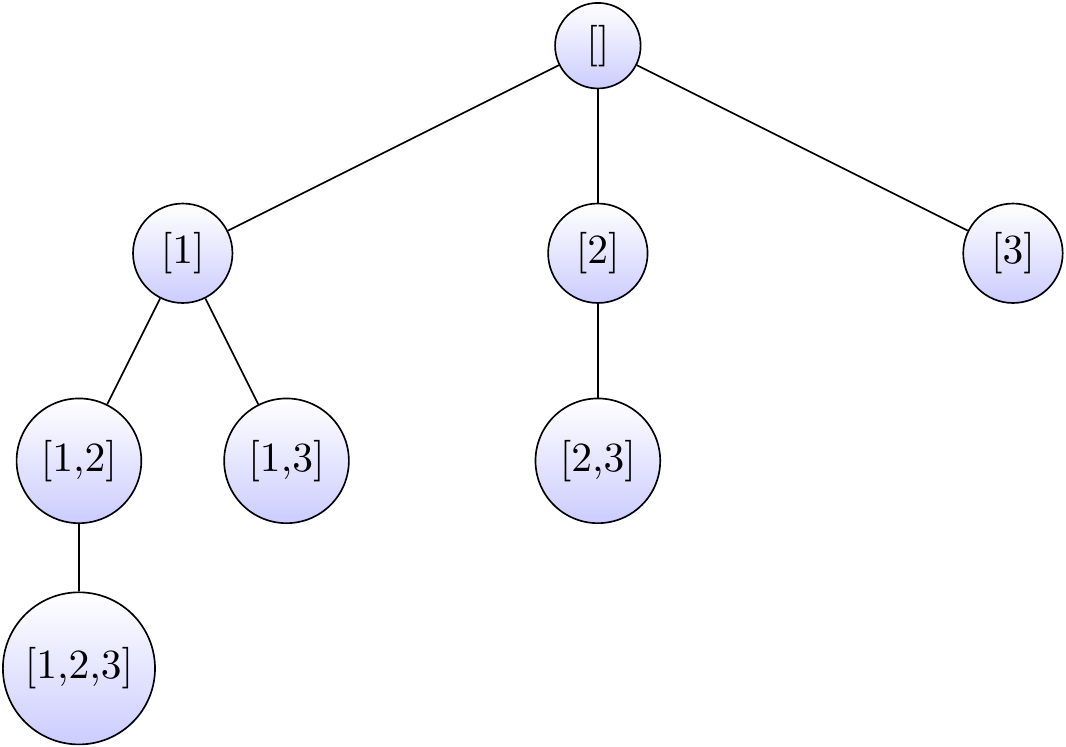
\includegraphics[width=0.9\linewidth]{tech-interview_files/figure-latex/unnamed-chunk-2-1} \caption{Some caption.}\label{fig:unnamed-chunk-2}
\end{figure}

Enumerate all possible result by adding a new element that is greater than current element while traversing the array.
Remember to backtrack.

\hypertarget{analysis-17}{%
\subsubsection{Analysis}\label{analysis-17}}

Time complexity between \(O(2^{n})\) as there are at most \(2^n\) subsets.

\hypertarget{algorithm-17}{%
\subsubsection{Algorithm}\label{algorithm-17}}

backtrack \ref{backtrack}, recursion \ref{recursion}

\hypertarget{java-code-13}{%
\subsection{Java Code}\label{java-code-13}}

\begin{Shaded}
\begin{Highlighting}[]
\BuiltInTok{List}\NormalTok{<}\BuiltInTok{List}\NormalTok{<}\BuiltInTok{Integer}\NormalTok{>> result = }\KeywordTok{new} \BuiltInTok{ArrayList}\NormalTok{<>();}

\KeywordTok{public} \BuiltInTok{List}\NormalTok{<}\BuiltInTok{List}\NormalTok{<}\BuiltInTok{Integer}\NormalTok{>> }\FunctionTok{subsets}\NormalTok{(}\DataTypeTok{int}\NormalTok{[] nums) \{}
    \KeywordTok{if}\NormalTok{ (nums.}\FunctionTok{length}\NormalTok{ == }\DecValTok{0}\NormalTok{) \{}
        \KeywordTok{return}\NormalTok{ result;}
\NormalTok{    \}}

    \BuiltInTok{Arrays}\NormalTok{.}\FunctionTok{sort}\NormalTok{(nums);}

    \FunctionTok{backtrack}\NormalTok{(nums, }\DecValTok{0}\NormalTok{, }\KeywordTok{new} \BuiltInTok{ArrayList}\NormalTok{<>());}

    \KeywordTok{return}\NormalTok{ result;}
\NormalTok{\}}

\KeywordTok{private} \DataTypeTok{void} \FunctionTok{backtrack}\NormalTok{(}\DataTypeTok{int}\NormalTok{[] nums, }\DataTypeTok{int}\NormalTok{ index, }\BuiltInTok{List}\NormalTok{<}\BuiltInTok{Integer}\NormalTok{> list) \{}
    \CommentTok{//copy elements from the current list}
\NormalTok{    result.}\FunctionTok{add}\NormalTok{(}\KeywordTok{new} \BuiltInTok{ArrayList}\NormalTok{<>(list));}

    \KeywordTok{for}\NormalTok{(}\DataTypeTok{int}\NormalTok{ i = index; i < nums.}\FunctionTok{length}\NormalTok{; i++) \{}
\NormalTok{        list.}\FunctionTok{add}\NormalTok{(nums[i]);}
        \FunctionTok{backtrack}\NormalTok{(nums, i + }\DecValTok{1}\NormalTok{, list);}

        \CommentTok{//remove last element to backtrack}
\NormalTok{        list.}\FunctionTok{remove}\NormalTok{(list.}\FunctionTok{size}\NormalTok{() - }\DecValTok{1}\NormalTok{);}
\NormalTok{    \}}
\NormalTok{\}}
\end{Highlighting}
\end{Shaded}

\hypertarget{subsets-ii-leetcode-90-medium}{%
\section{Subsets II / LeetCode 90 / Medium\}}\label{subsets-ii-leetcode-90-medium}}

\hypertarget{description-17}{%
\subsection{Description}\label{description-17}}

Given a collection of integers that might contain duplicates, nums, return all possible subsets (the power set).

Note: The solution set must not contain duplicate subsets.

\hypertarget{example-16}{%
\subsection{Example}\label{example-16}}

Input: nums = {[}1,2,2{]}, Output:

\begin{Shaded}
\begin{Highlighting}[]
\NormalTok{[}
\NormalTok{    [}\DecValTok{2}\NormalTok{],}
\NormalTok{    [}\DecValTok{1}\NormalTok{],}
\NormalTok{    [}\DecValTok{1}\NormalTok{,}\DecValTok{2}\NormalTok{,}\DecValTok{2}\NormalTok{],}
\NormalTok{    [}\DecValTok{2}\NormalTok{,}\DecValTok{2}\NormalTok{],}
\NormalTok{    [}\DecValTok{1}\NormalTok{,}\DecValTok{2}\NormalTok{],}
\NormalTok{    []}
\NormalTok{]}
\end{Highlighting}
\end{Shaded}

\hypertarget{solution-12}{%
\subsection{Solution}\label{solution-12}}

\hypertarget{walkthrough-16}{%
\subsubsection{Walkthrough}\label{walkthrough-16}}

The enumeration tree is as the following:

\begin{figure}
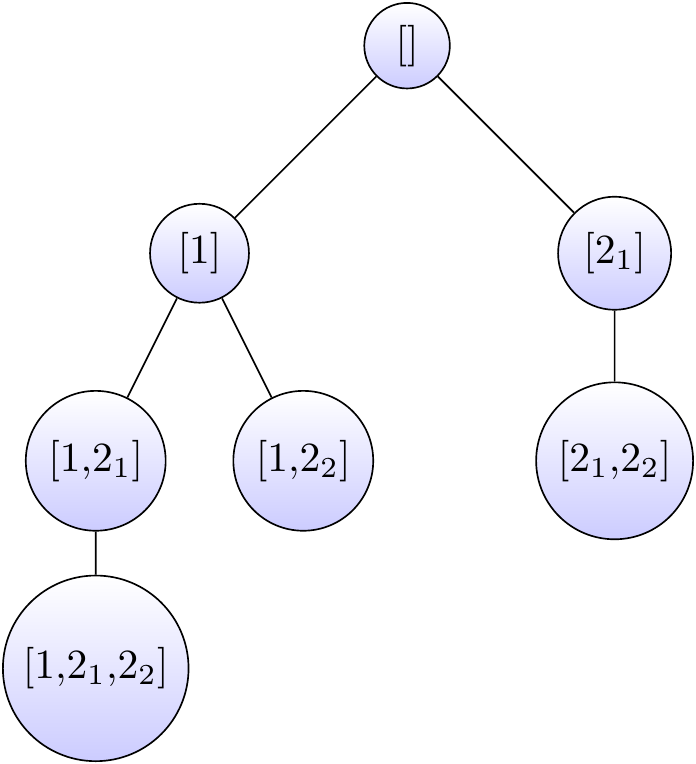
\includegraphics[width=0.9\linewidth]{tech-interview_files/figure-latex/unnamed-chunk-3-1} \caption{Some caption.}\label{fig:unnamed-chunk-3}
\end{figure}

Enumerate all possible result by adding a new element that is greater than current element while traversing the array.
Skip if two consecutive elements are the same. Remember to backtrack.

\hypertarget{analysis-18}{%
\subsubsection{Analysis}\label{analysis-18}}

Time complexity between \(O(2^{n})\) as there are at most \(2^n\) subsets.

\hypertarget{algorithm-18}{%
\subsubsection{Algorithm}\label{algorithm-18}}

backtrack \ref{backtrack}, recursion \ref{recursion}

\hypertarget{java-code-14}{%
\subsection{Java Code}\label{java-code-14}}

\begin{Shaded}
\begin{Highlighting}[]
\BuiltInTok{List}\NormalTok{<}\BuiltInTok{List}\NormalTok{<}\BuiltInTok{Integer}\NormalTok{>> result = }\KeywordTok{new} \BuiltInTok{ArrayList}\NormalTok{<>();}

\KeywordTok{public} \BuiltInTok{List}\NormalTok{<}\BuiltInTok{List}\NormalTok{<}\BuiltInTok{Integer}\NormalTok{>> }\FunctionTok{subsetsWithDup}\NormalTok{(}\DataTypeTok{int}\NormalTok{[] nums) \{}
    \KeywordTok{if}\NormalTok{ (nums.}\FunctionTok{length}\NormalTok{ == }\DecValTok{0}\NormalTok{) \{}
        \KeywordTok{return}\NormalTok{ result;}
\NormalTok{    \}}

    \BuiltInTok{Arrays}\NormalTok{.}\FunctionTok{sort}\NormalTok{(nums);}
    \FunctionTok{backtrack}\NormalTok{(nums, }\DecValTok{0}\NormalTok{, }\KeywordTok{new} \BuiltInTok{ArrayList}\NormalTok{<>());}

    \KeywordTok{return}\NormalTok{ result;}
\NormalTok{\}}

\KeywordTok{private} \DataTypeTok{void} \FunctionTok{backtrack}\NormalTok{(}\DataTypeTok{int}\NormalTok{[] nums, }\DataTypeTok{int}\NormalTok{ index, }\BuiltInTok{List}\NormalTok{<}\BuiltInTok{Integer}\NormalTok{> list) \{}
    \CommentTok{//copy elements from the current list}
\NormalTok{    result.}\FunctionTok{add}\NormalTok{(}\KeywordTok{new} \BuiltInTok{ArrayList}\NormalTok{<>(list));}

    \KeywordTok{for}\NormalTok{(}\DataTypeTok{int}\NormalTok{ i = index; i < nums.}\FunctionTok{length}\NormalTok{; i++) \{}
        \KeywordTok{if}\NormalTok{(i != index && nums[i] == nums[i - }\DecValTok{1}\NormalTok{]) \{}
            \KeywordTok{continue}\NormalTok{;}
\NormalTok{        \}}

\NormalTok{        list.}\FunctionTok{add}\NormalTok{(nums[i]);}
        \FunctionTok{backtrack}\NormalTok{(nums, i + }\DecValTok{1}\NormalTok{, list);}

        \CommentTok{//remove last element to backtrack}
\NormalTok{        list.}\FunctionTok{remove}\NormalTok{(list.}\FunctionTok{size}\NormalTok{() - }\DecValTok{1}\NormalTok{);}
\NormalTok{    \}}
\NormalTok{\}}
\end{Highlighting}
\end{Shaded}

\hypertarget{sort-array-by-parity-leetcode-906-easy}{%
\section{Sort Array By Parity / LeetCode 906 / Easy\}}\label{sort-array-by-parity-leetcode-906-easy}}

\hypertarget{description-18}{%
\subsection{Description}\label{description-18}}

Given an array A of non-negative integers, return an array consisting of all the even elements of A, followed by all
the odd elements of A.

You may return any answer array that satisfies this condition.

\hypertarget{example-17}{%
\subsection{Example}\label{example-17}}

Input: {[}3,1,2,4{]}. Output: {[}2,4,3,1{]}. The outputs {[}4,2,3,1{]}, {[}2,4,1,3{]}, and {[}4,2,1,3{]} would also be accepted.

\hypertarget{solution-13}{%
\subsection{Solution}\label{solution-13}}

\hypertarget{walkthrough-17}{%
\subsubsection{Walkthrough}\label{walkthrough-17}}

Have two indices, left and right. Shrink both indices (left, right) where they satisfy the condition. Swap those
who do not and shrink both indices again.

\hypertarget{analysis-19}{%
\subsubsection{Analysis}\label{analysis-19}}

Complexity is \(O(n)\) since each element is visited once.

\hypertarget{algorithm-19}{%
\subsubsection{Algorithm}\label{algorithm-19}}

\hypertarget{java-code-15}{%
\subsection{Java Code}\label{java-code-15}}

\begin{Shaded}
\begin{Highlighting}[]
\KeywordTok{public} \DataTypeTok{int}\NormalTok{[] }\FunctionTok{sortArrayByParity}\NormalTok{(}\DataTypeTok{int}\NormalTok{[] A) \{}
    \KeywordTok{if}\NormalTok{(A == }\KeywordTok{null}\NormalTok{ || A.}\FunctionTok{length}\NormalTok{ == }\DecValTok{0}\NormalTok{) \{}
        \KeywordTok{return} \KeywordTok{null}\NormalTok{;}
\NormalTok{    \}}

    \DataTypeTok{int}\NormalTok{ l = }\DecValTok{0}\NormalTok{, r = A.}\FunctionTok{length}\NormalTok{ - }\DecValTok{1}\NormalTok{;}
    \KeywordTok{while}\NormalTok{(l < r) \{}
        \KeywordTok{while}\NormalTok{ (A[l]%}\DecValTok{2}\NormalTok{ == }\DecValTok{0}\NormalTok{ && l < r) \{}
            \CommentTok{//do nothing, incremnt left index}
\NormalTok{            l++;}
\NormalTok{        \}}

        \KeywordTok{while}\NormalTok{ (A[r]%}\DecValTok{2}\NormalTok{ == }\DecValTok{1}\NormalTok{ && l < r) \{}
            \CommentTok{//do nothing, decrement right index}
\NormalTok{            r--;}
\NormalTok{        \}}


        \KeywordTok{if}\NormalTok{( l < r ) \{}
            \CommentTok{//odd #, swap}
            \DataTypeTok{int}\NormalTok{ temp = A[l];}
\NormalTok{            A[l] = A[r];}
\NormalTok{            A[r] = temp;}

\NormalTok{            l++;}
\NormalTok{            r--;}
\NormalTok{        \}}
\NormalTok{    \}}

    \KeywordTok{return}\NormalTok{ A;}
\NormalTok{\}}
\end{Highlighting}
\end{Shaded}

\hypertarget{merge-intervals-leetcode-56-medium}{%
\section{Merge Intervals / LeetCode 56 / Medium\}}\label{merge-intervals-leetcode-56-medium}}

\hypertarget{description-19}{%
\subsection{Description}\label{description-19}}

Given a collection of intervals, merge all overlapping intervals.

\hypertarget{example-18}{%
\subsection{Example}\label{example-18}}

Input: {[}{[}1,3{]},{[}2,6{]},{[}8,10{]},{[}15,18{]}{]}. Output: {[}{[}1,6{]},{[}8,10{]},{[}15,18{]}{]}. Explanation: Since intervals {[}1,3{]} and {[}2,6{]} overlaps, merge them into {[}1,6{]}.

Input: {[}{[}1,4{]},{[}4,5{]}{]}. Output: {[}{[}1,5{]}{]}. Explanation: Intervals {[}1,4{]} and {[}4,5{]} are considered overlapping.

\hypertarget{solution-14}{%
\subsection{Solution}\label{solution-14}}

\hypertarget{walkthrough-18}{%
\subsubsection{Walkthrough}\label{walkthrough-18}}

Sort the list of intervals first. Use a stack to track the lastly pushed interval. If the current interval does
not overlap with the top interval, push current interval to stack. If there is an overlap, we merge the
current and previous interval.

\hypertarget{analysis-20}{%
\subsubsection{Analysis}\label{analysis-20}}

Complexity is : \(O(n \cdot log n)\) since we sort the array first.

\hypertarget{algorithm-20}{%
\subsubsection{Algorithm}\label{algorithm-20}}

\hypertarget{java-code-16}{%
\subsection{Java Code}\label{java-code-16}}

\begin{Shaded}
\begin{Highlighting}[]
\DataTypeTok{static} \KeywordTok{class}\NormalTok{ Interval \{}
    \DataTypeTok{int}\NormalTok{ start;}
    \DataTypeTok{int}\NormalTok{ end;}

    \KeywordTok{public} \FunctionTok{Interval}\NormalTok{(}\DataTypeTok{int}\NormalTok{ l, }\DataTypeTok{int}\NormalTok{ r) \{}
\NormalTok{        start = l;}
\NormalTok{        end = r;}
\NormalTok{    \}}
\NormalTok{\}}

\KeywordTok{public} \DataTypeTok{int}\NormalTok{[][] }\FunctionTok{merge}\NormalTok{(}\DataTypeTok{int}\NormalTok{[][] intervals) \{}
    \BuiltInTok{List}\NormalTok{<Interval> input = }\KeywordTok{new} \BuiltInTok{ArrayList}\NormalTok{<>();}
    \KeywordTok{for}\NormalTok{(}\DataTypeTok{int}\NormalTok{[] interval : intervals) \{}
\NormalTok{        input.}\FunctionTok{add}\NormalTok{(}\KeywordTok{new} \FunctionTok{Interval}\NormalTok{(interval[}\DecValTok{0}\NormalTok{], interval[}\DecValTok{1}\NormalTok{]));}
\NormalTok{    \}}

    \KeywordTok{if}\NormalTok{(intervals.}\FunctionTok{length}\NormalTok{ == }\DecValTok{0}\NormalTok{) \{}
        \KeywordTok{return} \KeywordTok{new} \DataTypeTok{int}\NormalTok{[}\DecValTok{0}\NormalTok{][}\DecValTok{0}\NormalTok{];}
\NormalTok{    \}}

    \BuiltInTok{List}\NormalTok{<Interval> output = }\FunctionTok{merge}\NormalTok{(input);}
    \DataTypeTok{int}\NormalTok{[][] result = }\KeywordTok{new} \DataTypeTok{int}\NormalTok{[output.}\FunctionTok{size}\NormalTok{()][}\DecValTok{2}\NormalTok{];}

    \KeywordTok{for}\NormalTok{(}\DataTypeTok{int}\NormalTok{ i = }\DecValTok{0}\NormalTok{; i < output.}\FunctionTok{size}\NormalTok{(); i++) \{}
\NormalTok{        result[i][}\DecValTok{0}\NormalTok{] = output.}\FunctionTok{get}\NormalTok{(i).}\FunctionTok{start}\NormalTok{;}
\NormalTok{        result[i][}\DecValTok{1}\NormalTok{] = output.}\FunctionTok{get}\NormalTok{(i).}\FunctionTok{end}\NormalTok{;}
\NormalTok{    \}}

    \KeywordTok{return}\NormalTok{ result;}
\NormalTok{\}}

\KeywordTok{private} \KeywordTok{class}\NormalTok{ IntervalComparator }\KeywordTok{implements} \BuiltInTok{Comparator}\NormalTok{<Interval> \{}
    \AttributeTok{@Override}
    \KeywordTok{public} \DataTypeTok{int} \FunctionTok{compare}\NormalTok{(Interval a, Interval b) \{}
        \KeywordTok{return}\NormalTok{ a.}\FunctionTok{start}\NormalTok{ - b.}\FunctionTok{start}\NormalTok{;}
\NormalTok{    \}}
\NormalTok{\}}

\KeywordTok{public} \BuiltInTok{List}\NormalTok{<Interval> }\FunctionTok{merge}\NormalTok{(}\BuiltInTok{List}\NormalTok{<Interval> intervals) \{}
    \CommentTok{//sort the list}
    \BuiltInTok{Collections}\NormalTok{.}\FunctionTok{sort}\NormalTok{(intervals, }\KeywordTok{new} \FunctionTok{IntervalComparator}\NormalTok{());}

    \BuiltInTok{Stack}\NormalTok{<Interval> merged = }\KeywordTok{new} \BuiltInTok{Stack}\NormalTok{<Interval>();}
\NormalTok{    merged.}\FunctionTok{push}\NormalTok{(intervals.}\FunctionTok{get}\NormalTok{(}\DecValTok{0}\NormalTok{));}

    \KeywordTok{for}\NormalTok{ (}\DataTypeTok{int}\NormalTok{ i = }\DecValTok{1}\NormalTok{; i < intervals.}\FunctionTok{size}\NormalTok{(); i++) \{}
\NormalTok{        Interval interval = intervals.}\FunctionTok{get}\NormalTok{(i);}
\NormalTok{        Interval top = merged.}\FunctionTok{peek}\NormalTok{();}

        \CommentTok{// if interval does not overlap with the previous, simply append it.}
        \KeywordTok{if}\NormalTok{ (top.}\FunctionTok{end}\NormalTok{ < interval.}\FunctionTok{start}\NormalTok{) \{}
\NormalTok{            merged.}\FunctionTok{push}\NormalTok{(interval);}
\NormalTok{        \}}
        \CommentTok{// if there is an overlap, we merge the current with the last interval}
        \CommentTok{// by comparing their end boundaries}
        \KeywordTok{else}\NormalTok{ \{}
\NormalTok{            top.}\FunctionTok{end}\NormalTok{ = }\BuiltInTok{Math}\NormalTok{.}\FunctionTok{max}\NormalTok{(top.}\FunctionTok{end}\NormalTok{, interval.}\FunctionTok{end}\NormalTok{);}
\NormalTok{        \}}
\NormalTok{    \}}

    \KeywordTok{return}\NormalTok{ merged;}
\NormalTok{\}}
\end{Highlighting}
\end{Shaded}

\hypertarget{non-overlapping-intervals-leetcode-435-medium}{%
\section{Non-overlapping Intervals / LeetCode 435 / Medium\}}\label{non-overlapping-intervals-leetcode-435-medium}}

\hypertarget{description-20}{%
\subsection{Description}\label{description-20}}

Given a collection of intervals, find the minimum number of intervals you need to remove to make the rest of the
intervals non-overlapping.

\hypertarget{example-19}{%
\subsection{Example}\label{example-19}}

Input: {[}{[}1,2{]},{[}2,3{]},{[}3,4{]},{[}1,3{]}{]}. Output: 1 Explanation: {[}1,3{]} can be removed and the rest of intervals are
non-overlapping.

Input: {[}{[}1,2{]},{[}1,2{]},{[}1,2{]}{]}. Output: 2 . Explanation: You need to remove two {[}1,2{]} to make the rest of intervals
non-overlapping.

\hypertarget{solution-15}{%
\subsection{Solution}\label{solution-15}}

\hypertarget{walkthrough-19}{%
\subsubsection{Walkthrough}\label{walkthrough-19}}

First, sort the array and count non-overlapping interval - not overlapped with previous end. Finally, number of
overlapping intervals would be n - count.

\hypertarget{analysis-21}{%
\subsubsection{Analysis}\label{analysis-21}}

Complexity is \(O(n \cdot log n)\) because of sorting ahead.

\hypertarget{algorithm-21}{%
\subsubsection{Algorithm}\label{algorithm-21}}

\hypertarget{java-code-17}{%
\subsection{Java Code}\label{java-code-17}}

\begin{Shaded}
\begin{Highlighting}[]
\KeywordTok{public} \DataTypeTok{int} \FunctionTok{eraseOverlapIntervals}\NormalTok{(}\DataTypeTok{int}\NormalTok{[][] intervals) \{}
    \KeywordTok{if}\NormalTok{(intervals == }\KeywordTok{null}\NormalTok{ || intervals.}\FunctionTok{length}\NormalTok{ == }\DecValTok{0}\NormalTok{) \{}
        \KeywordTok{return} \DecValTok{0}\NormalTok{;}
\NormalTok{    \}}

    \BuiltInTok{Arrays}\NormalTok{.}\FunctionTok{sort}\NormalTok{(intervals, }\KeywordTok{new} \BuiltInTok{Comparator}\NormalTok{<}\DataTypeTok{int}\NormalTok{[]>() \{}
        \AttributeTok{@Override}
        \KeywordTok{public} \DataTypeTok{int} \FunctionTok{compare}\NormalTok{(}\DataTypeTok{int}\NormalTok{[] i1, }\DataTypeTok{int}\NormalTok{[] i2) \{}
            \KeywordTok{if}\NormalTok{ (i1[}\DecValTok{1}\NormalTok{] != i2[}\DecValTok{1}\NormalTok{])\{}
                \CommentTok{//compare end time}
                \KeywordTok{return}\NormalTok{ i1[}\DecValTok{1}\NormalTok{] - i2[}\DecValTok{1}\NormalTok{];}
\NormalTok{            \}}\KeywordTok{else}\NormalTok{ \{}
                \CommentTok{//compare start time}
                \KeywordTok{return}\NormalTok{ i1[}\DecValTok{0}\NormalTok{] - i2[}\DecValTok{0}\NormalTok{];}
\NormalTok{            \}}
\NormalTok{        \}}
\NormalTok{    \});}

    \CommentTok{//end for latest non-overlapped interval}
    \DataTypeTok{int}\NormalTok{ end = intervals[}\DecValTok{0}\NormalTok{][}\DecValTok{1}\NormalTok{];}
    \DataTypeTok{int}\NormalTok{ n = intervals.}\FunctionTok{length}\NormalTok{;}
    \DataTypeTok{int}\NormalTok{ count = }\DecValTok{1}\NormalTok{;}

    \KeywordTok{for}\NormalTok{ (}\DataTypeTok{int}\NormalTok{ i = }\DecValTok{1}\NormalTok{; i < n; i++) \{}
        \KeywordTok{if}\NormalTok{ (intervals[i][}\DecValTok{0}\NormalTok{] >= end) \{}
            \CommentTok{//for any non-overlapped interval, update end & count}
\NormalTok{            end = intervals[i][}\DecValTok{1}\NormalTok{];}
\NormalTok{            count++;}
\NormalTok{        \}}
\NormalTok{    \}}

    \KeywordTok{return}\NormalTok{ n - count;}
\NormalTok{\}}
\end{Highlighting}
\end{Shaded}

\hypertarget{interval-list-intersections-leetcode-986-medium}{%
\section{Interval List Intersections / LeetCode 986 / Medium\}}\label{interval-list-intersections-leetcode-986-medium}}

\hypertarget{description-21}{%
\subsection{Description}\label{description-21}}

Given two lists of closed intervals, each list of intervals is pairwise disjoint and in sorted order.
Return the intersection of these two interval lists.

\hypertarget{example-20}{%
\subsection{Example}\label{example-20}}

Input: A = {[}{[}0,2{]},{[}5,10{]},{[}13,23{]},{[}24,25{]}{]}, B = {[}{[}1,5{]},{[}8,12{]},{[}15,24{]},{[}25,26{]}{]}
Output: {[}{[}1,2{]},{[}5,5{]},{[}8,10{]},{[}15,23{]},{[}24,24{]},{[}25,25{]}{]}
Reminder: The inputs and the desired output are lists of Interval objects, and not arrays or lists.

\hypertarget{solution-16}{%
\subsection{Solution}\label{solution-16}}

\hypertarget{walkthrough-20}{%
\subsubsection{Walkthrough}\label{walkthrough-20}}

Traverse the two lists of intervals. Merge two intervals if there is an intersection. Move the index of A if
\(A[i]\).end \(< B[i]\).end since the interval is the smaller out of comparison.

\hypertarget{analysis-22}{%
\subsubsection{Analysis}\label{analysis-22}}

The runtime complexity is \(O(n * m)\)

\hypertarget{algorithm-22}{%
\subsubsection{Algorithm}\label{algorithm-22}}

\hypertarget{java-code-18}{%
\subsection{Java Code}\label{java-code-18}}

\begin{Shaded}
\begin{Highlighting}[]
\NormalTok{LeetCode }\DecValTok{986}\NormalTok{ / Medium}
\KeywordTok{private} \DataTypeTok{static} \KeywordTok{class}\NormalTok{ Interval \{}
    \KeywordTok{public} \DataTypeTok{int}\NormalTok{ start;}
    \KeywordTok{public} \DataTypeTok{int}\NormalTok{ end;}

    \KeywordTok{public} \FunctionTok{Interval}\NormalTok{(}\DataTypeTok{int}\NormalTok{ s, }\DataTypeTok{int}\NormalTok{ e) \{}
        \KeywordTok{this}\NormalTok{.}\FunctionTok{start}\NormalTok{ = s;}
        \KeywordTok{this}\NormalTok{.}\FunctionTok{end}\NormalTok{ = e;}
\NormalTok{    \}}

    \KeywordTok{public} \DataTypeTok{static} \DataTypeTok{int}\NormalTok{[][] }\FunctionTok{toArray}\NormalTok{(}\BuiltInTok{List}\NormalTok{<Interval> list) \{}
        \DataTypeTok{int}\NormalTok{[][] result = }\KeywordTok{new} \DataTypeTok{int}\NormalTok{[list.}\FunctionTok{size}\NormalTok{()][}\DecValTok{2}\NormalTok{];}

        \KeywordTok{for}\NormalTok{(}\DataTypeTok{int}\NormalTok{ i = }\DecValTok{0}\NormalTok{; i < list.}\FunctionTok{size}\NormalTok{(); i++) \{}
\NormalTok{            Interval interval = list.}\FunctionTok{get}\NormalTok{(i);}

\NormalTok{            result[i] = }\KeywordTok{new} \DataTypeTok{int}\NormalTok{[] \{interval.}\FunctionTok{start}\NormalTok{, interval.}\FunctionTok{end}\NormalTok{\};}
\NormalTok{        \}}

        \KeywordTok{return}\NormalTok{ result;}
\NormalTok{    \}}

    \KeywordTok{public} \DataTypeTok{static} \BuiltInTok{List}\NormalTok{<Interval> }\FunctionTok{toList}\NormalTok{(}\DataTypeTok{int}\NormalTok{[][] array) \{}
        \BuiltInTok{List}\NormalTok{<Interval> result = }\KeywordTok{new} \BuiltInTok{ArrayList}\NormalTok{<>();}

        \KeywordTok{for}\NormalTok{(}\DataTypeTok{int}\NormalTok{ i = }\DecValTok{0}\NormalTok{; i < array.}\FunctionTok{length}\NormalTok{; i++) \{}
\NormalTok{            Interval interval = }\KeywordTok{new} \FunctionTok{Interval}\NormalTok{(array[i][}\DecValTok{0}\NormalTok{], array[i][}\DecValTok{1}\NormalTok{]);}

\NormalTok{            result.}\FunctionTok{add}\NormalTok{(interval);}
\NormalTok{        \}}

        \KeywordTok{return}\NormalTok{ result;}
\NormalTok{    \}}

\NormalTok{\}}
\KeywordTok{public} \DataTypeTok{int}\NormalTok{[][] }\FunctionTok{intervalIntersection}\NormalTok{(}\DataTypeTok{int}\NormalTok{[][] A, }\DataTypeTok{int}\NormalTok{[][] B) \{}
    \BuiltInTok{List}\NormalTok{<Interval> intervalsA = Interval.}\FunctionTok{toList}\NormalTok{(A);}
    \BuiltInTok{List}\NormalTok{<Interval> intervalsB = Interval.}\FunctionTok{toList}\NormalTok{(B);}
    \BuiltInTok{List}\NormalTok{<Interval> result = }\KeywordTok{new} \BuiltInTok{ArrayList}\NormalTok{<>();}

    \DataTypeTok{int}\NormalTok{ i = }\DecValTok{0}\NormalTok{, j = }\DecValTok{0}\NormalTok{;}
    \KeywordTok{while}\NormalTok{( i < intervalsA.}\FunctionTok{size}\NormalTok{() && j < intervalsB.}\FunctionTok{size}\NormalTok{()) \{}
        \DataTypeTok{int}\NormalTok{ highStart = }\BuiltInTok{Math}\NormalTok{.}\FunctionTok{max}\NormalTok{(intervalsA.}\FunctionTok{get}\NormalTok{(i).}\FunctionTok{start}\NormalTok{, intervalsB.}\FunctionTok{get}\NormalTok{(j).}\FunctionTok{start}\NormalTok{);}
        \DataTypeTok{int}\NormalTok{ lowEnd = }\BuiltInTok{Math}\NormalTok{.}\FunctionTok{min}\NormalTok{(intervalsA.}\FunctionTok{get}\NormalTok{(i).}\FunctionTok{end}\NormalTok{, intervalsB.}\FunctionTok{get}\NormalTok{(j).}\FunctionTok{end}\NormalTok{);}

        \CommentTok{//there is an intersection}
        \KeywordTok{if}\NormalTok{( highStart <= lowEnd) \{}
\NormalTok{            result.}\FunctionTok{add}\NormalTok{( }\KeywordTok{new} \FunctionTok{Interval}\NormalTok{(highStart, lowEnd));}
\NormalTok{        \}}
        \KeywordTok{if}\NormalTok{( intervalsA.}\FunctionTok{get}\NormalTok{(i).}\FunctionTok{end}\NormalTok{ < intervalsB.}\FunctionTok{get}\NormalTok{(j).}\FunctionTok{end}\NormalTok{) \{}
            \CommentTok{//move index of A[]}
\NormalTok{            i++;}
\NormalTok{        \} }\KeywordTok{else}\NormalTok{ \{}
            \CommentTok{//move index of B[]}
\NormalTok{            j++;}
\NormalTok{        \}}
\NormalTok{    \}}

    \KeywordTok{return}\NormalTok{ Interval.}\FunctionTok{toArray}\NormalTok{(result);}
\NormalTok{\}}
\end{Highlighting}
\end{Shaded}

\hypertarget{insert-interval-leetcode-57-hard}{%
\section{Insert Interval / LeetCode 57 / Hard\}}\label{insert-interval-leetcode-57-hard}}

\hypertarget{description-22}{%
\subsection{Description}\label{description-22}}

Given a set of non-overlapping intervals, insert a new interval into the intervals (merge if necessary).

You may assume that the intervals were initially sorted according to their start times.

\hypertarget{example-21}{%
\subsection{Example}\label{example-21}}

Input: intervals = {[}{[}1,3{]},{[}6,9{]}{]}, newInterval = {[}2,5{]} Output: {[}{[}1,5{]},{[}6,9{]}{]}

Input: intervals = {[}{[}1,2{]},{[}3,5{]},{[}6,7{]},{[}8,10{]},{[}12,16{]}{]}, newInterval = {[}4,8{]}. Output: {[}{[}1,2{]},{[}3,10{]},{[}12,16{]}{]}
Explanation: Because the new interval {[}4,8{]} overlaps with {[}3,5{]},{[}6,7{]},{[}8,10{]}.

\hypertarget{solution-17}{%
\subsection{Solution}\label{solution-17}}

\hypertarget{walkthrough-21}{%
\subsubsection{Walkthrough}\label{walkthrough-21}}

Leverage the merge() method to find out which intervals can be merged with new Inserted interval.

\hypertarget{analysis-23}{%
\subsubsection{Analysis}\label{analysis-23}}

Time complexity is \(O(n \cdot log(n))\) because of sorting ahead.

\hypertarget{algorithm-23}{%
\subsubsection{Algorithm}\label{algorithm-23}}

\hypertarget{java-code-19}{%
\subsection{Java Code}\label{java-code-19}}

\begin{Shaded}
\begin{Highlighting}[]
\KeywordTok{private} \DataTypeTok{static} \KeywordTok{class}\NormalTok{ Interval \{}
    \KeywordTok{public} \DataTypeTok{int}\NormalTok{ start;}
    \KeywordTok{public} \DataTypeTok{int}\NormalTok{ end;}

    \KeywordTok{public} \FunctionTok{Interval}\NormalTok{(}\DataTypeTok{int}\NormalTok{ s, }\DataTypeTok{int}\NormalTok{ e) \{}
        \KeywordTok{this}\NormalTok{.}\FunctionTok{start}\NormalTok{ = s;}
        \KeywordTok{this}\NormalTok{.}\FunctionTok{end}\NormalTok{ = e;}
\NormalTok{    \}}

    \KeywordTok{public} \DataTypeTok{static} \DataTypeTok{int}\NormalTok{[][] }\FunctionTok{toArray}\NormalTok{(}\BuiltInTok{List}\NormalTok{<Interval> list) \{}
        \DataTypeTok{int}\NormalTok{[][] result = }\KeywordTok{new} \DataTypeTok{int}\NormalTok{[list.}\FunctionTok{size}\NormalTok{()][}\DecValTok{2}\NormalTok{];}

        \KeywordTok{for}\NormalTok{(}\DataTypeTok{int}\NormalTok{ i = }\DecValTok{0}\NormalTok{; i < list.}\FunctionTok{size}\NormalTok{(); i++) \{}
\NormalTok{            Interval interval = list.}\FunctionTok{get}\NormalTok{(i);}

\NormalTok{            result[i] = }\KeywordTok{new} \DataTypeTok{int}\NormalTok{[] \{interval.}\FunctionTok{start}\NormalTok{, interval.}\FunctionTok{end}\NormalTok{\};}
\NormalTok{        \}}

        \KeywordTok{return}\NormalTok{ result;}
\NormalTok{    \}}

    \KeywordTok{public} \DataTypeTok{static} \BuiltInTok{List}\NormalTok{<Interval> }\FunctionTok{toList}\NormalTok{(}\DataTypeTok{int}\NormalTok{[][] array) \{}
        \BuiltInTok{List}\NormalTok{<Interval> result = }\KeywordTok{new} \BuiltInTok{ArrayList}\NormalTok{<>();}

        \KeywordTok{for}\NormalTok{(}\DataTypeTok{int}\NormalTok{ i = }\DecValTok{0}\NormalTok{; i < array.}\FunctionTok{length}\NormalTok{; i++) \{}
\NormalTok{            Interval interval = }\KeywordTok{new} \FunctionTok{Interval}\NormalTok{(array[i][}\DecValTok{0}\NormalTok{], array[i][}\DecValTok{1}\NormalTok{]);}

\NormalTok{            result.}\FunctionTok{add}\NormalTok{(interval);}
\NormalTok{        \}}

        \KeywordTok{return}\NormalTok{ result;}
\NormalTok{    \}}
\NormalTok{\}}

\KeywordTok{public} \DataTypeTok{int}\NormalTok{[][] }\FunctionTok{insert}\NormalTok{(}\DataTypeTok{int}\NormalTok{[][] existed, }\DataTypeTok{int}\NormalTok{[] target) \{}
    \BuiltInTok{List}\NormalTok{<Interval> intervals = Interval.}\FunctionTok{toList}\NormalTok{(existed);}
\NormalTok{    Interval newInterval = }\KeywordTok{new} \FunctionTok{Interval}\NormalTok{(target[}\DecValTok{0}\NormalTok{], target[}\DecValTok{1}\NormalTok{]);}

\NormalTok{    intervals.}\FunctionTok{add}\NormalTok{(newInterval);}

    \BuiltInTok{List}\NormalTok{<Interval> merged = }\FunctionTok{merge}\NormalTok{(intervals);}

    \KeywordTok{return}\NormalTok{ Interval.}\FunctionTok{toArray}\NormalTok{(merged);}
\NormalTok{\}}

\KeywordTok{private} \KeywordTok{class}\NormalTok{ IntervalComparator }\KeywordTok{implements} \BuiltInTok{Comparator}\NormalTok{<Interval> \{}
    \AttributeTok{@Override}
    \KeywordTok{public} \DataTypeTok{int} \FunctionTok{compare}\NormalTok{(Interval a, Interval b) \{}
        \KeywordTok{return}\NormalTok{ a.}\FunctionTok{start}\NormalTok{ < b.}\FunctionTok{start}\NormalTok{ ? }\DecValTok{-1}\NormalTok{ : a.}\FunctionTok{start}\NormalTok{ == b.}\FunctionTok{start}\NormalTok{ ? }\DecValTok{0}\NormalTok{ : }\DecValTok{1}\NormalTok{;}
\NormalTok{    \}}
\NormalTok{\}}

\KeywordTok{public} \BuiltInTok{List}\NormalTok{<Interval> }\FunctionTok{merge}\NormalTok{(}\BuiltInTok{List}\NormalTok{<Interval> intervals) \{}
    \CommentTok{//sort the list}
    \BuiltInTok{Collections}\NormalTok{.}\FunctionTok{sort}\NormalTok{(intervals, }\KeywordTok{new} \FunctionTok{IntervalComparator}\NormalTok{());}

    \BuiltInTok{LinkedList}\NormalTok{<Interval> merged = }\KeywordTok{new} \BuiltInTok{LinkedList}\NormalTok{<Interval>();}
    \KeywordTok{for}\NormalTok{ (Interval interval : intervals) \{}
        \KeywordTok{if}\NormalTok{ (merged.}\FunctionTok{isEmpty}\NormalTok{() || merged.}\FunctionTok{getLast}\NormalTok{().}\FunctionTok{end}\NormalTok{ < interval.}\FunctionTok{start}\NormalTok{) \{}
            \CommentTok{// if the list of merged intervals is empty or if the current}
            \CommentTok{// interval does not overlap with the previous, simply append it.}
\NormalTok{            merged.}\FunctionTok{add}\NormalTok{(interval);}
\NormalTok{        \} }\KeywordTok{else}\NormalTok{ \{}
            \CommentTok{// otherwise, there is overlap, so we merge the current and previous}
            \CommentTok{// intervals.}
\NormalTok{            merged.}\FunctionTok{getLast}\NormalTok{().}\FunctionTok{end}\NormalTok{ = }\BuiltInTok{Math}\NormalTok{.}\FunctionTok{max}\NormalTok{(merged.}\FunctionTok{getLast}\NormalTok{().}\FunctionTok{end}\NormalTok{, interval.}\FunctionTok{end}\NormalTok{);}
\NormalTok{        \}}
\NormalTok{    \}}
    \KeywordTok{return}\NormalTok{ merged;}
\NormalTok{\}}
\end{Highlighting}
\end{Shaded}

\hypertarget{find-common-characters-leetcode-1002-easy}{%
\section{Find Common Characters / LeetCode 1002 / Easy\}}\label{find-common-characters-leetcode-1002-easy}}

\hypertarget{description-23}{%
\subsection{Description}\label{description-23}}

Given an array A of strings made only from lowercase letters, return a list of all characters that show up in all
strings within the list (including duplicates). For example, if a character occurs 3 times in all strings but
not 4 times, you need to include that character three times in the final answer. You may return the answer in
any order.

\hypertarget{example-22}{%
\subsection{Example}\label{example-22}}

Input: {[}``bella'',``label'',``roller''{]}. Output: {[}``e'',``l'',``l''{]}

Input: {[}``cool'',``lock'',``cook''{]}. Output: {[}``c'',``o''{]}

\hypertarget{solution-18}{%
\subsection{Solution}\label{solution-18}}

\hypertarget{walkthrough-22}{%
\subsubsection{Walkthrough}\label{walkthrough-22}}

First retrieve the alphabet distribution for the first word. For each of following word, maintain the min number
of duplicated alphabets. Lastly, take the alphabet which has more than 1 occurrences.

\hypertarget{analysis-24}{%
\subsubsection{Analysis}\label{analysis-24}}

Time complexity is O(n) where n is the number of words.

\hypertarget{algorithm-24}{%
\subsubsection{Algorithm}\label{algorithm-24}}

\hypertarget{java-code-20}{%
\subsection{Java Code}\label{java-code-20}}

\begin{Shaded}
\begin{Highlighting}[]
\KeywordTok{public} \BuiltInTok{List}\NormalTok{<}\BuiltInTok{String}\NormalTok{> }\FunctionTok{commonChars}\NormalTok{(}\BuiltInTok{String}\NormalTok{[] A) \{}
    \DataTypeTok{int}\NormalTok{[] minFreq = }\KeywordTok{new} \DataTypeTok{int}\NormalTok{[}\DecValTok{26}\NormalTok{];}

    \CommentTok{//init frequency map with the first string}
    \KeywordTok{for}\NormalTok{(}\DataTypeTok{int}\NormalTok{ i = }\DecValTok{0}\NormalTok{; i < A[}\DecValTok{0}\NormalTok{].}\FunctionTok{length}\NormalTok{(); i++) \{}
        \DataTypeTok{char}\NormalTok{ c = A[}\DecValTok{0}\NormalTok{].}\FunctionTok{charAt}\NormalTok{(i);}

        \DataTypeTok{int}\NormalTok{ index = c - }\CharTok{'a'}\NormalTok{;}
        \DataTypeTok{int}\NormalTok{ counter = minFreq[index];}
\NormalTok{        minFreq[index] = ++counter;}
\NormalTok{    \}}


    \CommentTok{//Do the actions for the following words}
    \KeywordTok{for}\NormalTok{(}\DataTypeTok{int}\NormalTok{ i = }\DecValTok{1}\NormalTok{; i < A.}\FunctionTok{length}\NormalTok{; i++) \{}
        \BuiltInTok{String}\NormalTok{ str = A[i];}
        \DataTypeTok{int}\NormalTok{[] tempFreq = }\KeywordTok{new} \DataTypeTok{int}\NormalTok{[}\DecValTok{26}\NormalTok{];}

        \CommentTok{//1. Store the frequency of alphabets}
        \KeywordTok{for}\NormalTok{(}\DataTypeTok{int}\NormalTok{ j = }\DecValTok{0}\NormalTok{; j < str.}\FunctionTok{length}\NormalTok{(); j++) \{}
            \DataTypeTok{char}\NormalTok{ c = str.}\FunctionTok{charAt}\NormalTok{(j);}

            \DataTypeTok{int}\NormalTok{ index = c - }\CharTok{'a'}\NormalTok{;}
            \DataTypeTok{int}\NormalTok{ counter = tempFreq[index];}
\NormalTok{            tempFreq[index] = ++counter;}
\NormalTok{        \}}

        \CommentTok{//2. Iterate thru 2 arrays and get the min number of (duplicated) alphabets}
        \CommentTok{//   non-duplicated returns 0}
        \KeywordTok{for}\NormalTok{(}\DataTypeTok{int}\NormalTok{ j = }\DecValTok{0}\NormalTok{; j < }\DecValTok{26}\NormalTok{; j++) \{}
\NormalTok{            minFreq[j] = }\BuiltInTok{Math}\NormalTok{.}\FunctionTok{min}\NormalTok{(minFreq[j], tempFreq[j]);}
\NormalTok{        \}}
\NormalTok{    \}}

    \DataTypeTok{int}\NormalTok{ numOfWords = A.}\FunctionTok{length}\NormalTok{;}
    \BuiltInTok{List}\NormalTok{<}\BuiltInTok{String}\NormalTok{> result = }\KeywordTok{new} \BuiltInTok{ArrayList}\NormalTok{<>();}


    \KeywordTok{for}\NormalTok{(}\DataTypeTok{int}\NormalTok{ i = }\DecValTok{0}\NormalTok{; i < }\DecValTok{26}\NormalTok{; i++) \{}
        \DataTypeTok{int}\NormalTok{ minCounter = minFreq[i];}

        \CommentTok{//Take the min number of duplicated alphabets (1 min)}
        \KeywordTok{for}\NormalTok{(}\DataTypeTok{int}\NormalTok{ j = }\DecValTok{0}\NormalTok{; j < minCounter; j++) \{}
            \DataTypeTok{char}\NormalTok{ alphabet = (}\DataTypeTok{char}\NormalTok{) (}\CharTok{'a'}\NormalTok{ + i);}
\NormalTok{            result.}\FunctionTok{add}\NormalTok{(}\BuiltInTok{String}\NormalTok{.}\FunctionTok{valueOf}\NormalTok{(alphabet));}
\NormalTok{        \}}
\NormalTok{    \}}

    \KeywordTok{return}\NormalTok{ result;}
\NormalTok{\}}
\end{Highlighting}
\end{Shaded}

\hypertarget{top-k-frequently-appeared-elements-leet-code-347-medium}{%
\section{Top K Frequently Appeared Elements / Leet Code 347 / Medium\}}\label{top-k-frequently-appeared-elements-leet-code-347-medium}}

\hypertarget{description-24}{%
\subsection{Description}\label{description-24}}

Given a non-empty array of integers, return the k most frequent elements. You may assume k is always valid,
\$1 \le k \le \$ number of unique elements. Your algorithm's time complexity must be better than O(\(n log n\)), where n
is the array's size.

\hypertarget{example-23}{%
\subsection{Example}\label{example-23}}

Input: nums = {[}1,1,1,2,2,3{]}, k = 2 Output: {[}1,2{]}
\#\#\# Solution
\#\#\#\# Walkthrough

\begin{verbatim}
* We first gather the frequency of integer by count with a HashMap
* We sort the frequency map by comparing by value() in descending order and sort them in
$List<Entry<Number, Frequency>>$.
* We could traverse the top K entries from the list in a loop.
\end{verbatim}

\hypertarget{analysis-25}{%
\subsubsection{Analysis}\label{analysis-25}}

Since we sort the frequency map, thus the time complexity is \(O(n \cdot log n)\), and Auxiliary Space is \(O(n)\) to
store several maps and list.

\hypertarget{algorithm-25}{%
\subsubsection{Algorithm}\label{algorithm-25}}

\hypertarget{java-code-21}{%
\subsection{Java Code}\label{java-code-21}}

\begin{Shaded}
\begin{Highlighting}[]
\KeywordTok{public} \BuiltInTok{List}\NormalTok{<}\BuiltInTok{Integer}\NormalTok{> }\FunctionTok{topKFrequent}\NormalTok{(}\DataTypeTok{int}\NormalTok{[] nums, }\DataTypeTok{int}\NormalTok{ k) \{}
    \BuiltInTok{Map}\NormalTok{<}\BuiltInTok{Integer}\NormalTok{, }\BuiltInTok{Integer}\NormalTok{> freq = }\KeywordTok{new} \BuiltInTok{HashMap}\NormalTok{<>();}

    \KeywordTok{for}\NormalTok{ (}\DataTypeTok{int}\NormalTok{ num : nums) \{}
        \DataTypeTok{int}\NormalTok{ count = freq.}\FunctionTok{getOrDefault}\NormalTok{(num, }\DecValTok{0}\NormalTok{);}
\NormalTok{        freq.}\FunctionTok{put}\NormalTok{(num, ++count);}
\NormalTok{    \}}

    \CommentTok{//Sort Map.Entry by comparing by value() in descending order}
    \BuiltInTok{List}\NormalTok{<}\BuiltInTok{Map}\NormalTok{.}\FunctionTok{Entry}\NormalTok{<}\BuiltInTok{Integer}\NormalTok{, }\BuiltInTok{Integer}\NormalTok{>> sortedList = }\KeywordTok{new} \BuiltInTok{ArrayList}\NormalTok{<>(freq.}\FunctionTok{entrySet}\NormalTok{());}
\NormalTok{    sortedList.}\FunctionTok{sort}\NormalTok{(}\BuiltInTok{Map}\NormalTok{.}\FunctionTok{Entry}\NormalTok{.}\FunctionTok{comparingByValue}\NormalTok{(}\BuiltInTok{Comparator}\NormalTok{.}\FunctionTok{reverseOrder}\NormalTok{()));}


    \BuiltInTok{List}\NormalTok{<}\BuiltInTok{Integer}\NormalTok{> result = }\KeywordTok{new} \BuiltInTok{ArrayList}\NormalTok{<>();}
    \DataTypeTok{int}\NormalTok{ topN = }\DecValTok{0}\NormalTok{;}

    \KeywordTok{for}\NormalTok{ (}\BuiltInTok{Map}\NormalTok{.}\FunctionTok{Entry}\NormalTok{<}\BuiltInTok{Integer}\NormalTok{, }\BuiltInTok{Integer}\NormalTok{> entry : sortedList) \{}
        \CommentTok{//Top K elements retrieved}
        \KeywordTok{if}\NormalTok{(topN == k) \{}
            \KeywordTok{break}\NormalTok{;}
\NormalTok{        \}}

\NormalTok{        result.}\FunctionTok{add}\NormalTok{(entry.}\FunctionTok{getKey}\NormalTok{());}
\NormalTok{        topN++;}
\NormalTok{    \}}

    \KeywordTok{return}\NormalTok{ result;}
\NormalTok{\}}
\end{Highlighting}
\end{Shaded}

\hypertarget{count-iterations-towards-filling-1s-in-an-array}{%
\section{Count iterations towards filling 1's in an array / / \}}\label{count-iterations-towards-filling-1s-in-an-array}}

\hypertarget{description-25}{%
\subsection{Description}\label{description-25}}

Given an array of 0s and 1s, in how many iterations the whole array can be filled with 1s if in a single iteration
immediate neighbors of 1s can be filled. If we cannot fill array with 1s, then print ``-1''

\hypertarget{example-24}{%
\subsection{Example}\label{example-24}}

Input : arr{[}{]} = \{1, 0, 1, 0, 0, 1, 0, 1, 1, 0, 1, 1, 0, 0, 1\}
Output : 1

Input : arr{[}{]} = \{0, 0, 1, 1, 0, 0, 1, 1, 0, 1, 1, 1, 1, 0, 0, 0, 1\}
Output : 2

\hypertarget{solution-19}{%
\subsection{Solution}\label{solution-19}}

\hypertarget{walkthrough-23}{%
\subsubsection{Walkthrough}\label{walkthrough-23}}

For each sub-block of the array, consider the following 3 scenarios

\begin{verbatim}
* Case 1: There are no 1's. In this case, array cannot be filled with 1's. Thus, return -1;
* Locate the first 1 and evalute the following
    
        * Case 2: [1, 0, 0, ...., 0, 1] Another 1 follows and makes it a block of 0s with 1s on both ends. Number of iteration needed
\end{verbatim}

to flip the 0s become \(num_zeo / 2\) if number is even otherwise \((num_zero + 1) / 2\)
* Case 3: {[}1, 0, 0, \ldots{}, 0{]} Another 1 cannot be found and makes it a single 1 at the end. Number of iteration needed equals
to the number of 0s.

\begin{verbatim}
* Case 3: [0, 0, 0, ..., 1] Count the number of 0s until the first 1 is met.
\end{verbatim}

Finally, we need to get the maximum iteration for each subproblems.

\hypertarget{analysis-26}{%
\subsubsection{Analysis}\label{analysis-26}}

Time Complexity : O(n) since every element is visited once.

\hypertarget{algorithm-26}{%
\subsubsection{Algorithm}\label{algorithm-26}}

\hypertarget{java-code-22}{%
\subsection{Java Code}\label{java-code-22}}

\begin{Shaded}
\begin{Highlighting}[]
\DataTypeTok{int} \FunctionTok{countIterations}\NormalTok{(}\DataTypeTok{int}\NormalTok{ arr[]) \{}
    \DataTypeTok{boolean}\NormalTok{ oneFound = }\KeywordTok{false}\NormalTok{;}
    \DataTypeTok{int}\NormalTok{ maxIteration = }\DecValTok{0}\NormalTok{;}

    \DataTypeTok{int}\NormalTok{ n = arr.}\FunctionTok{length}\NormalTok{;}
    \DataTypeTok{int}\NormalTok{ i = }\DecValTok{0}\NormalTok{;}

    \CommentTok{// Start traversing the array}
    \KeywordTok{while}\NormalTok{ ( i < n ) \{}
        \KeywordTok{if}\NormalTok{ (arr[i] == }\DecValTok{1}\NormalTok{) \{}
\NormalTok{            oneFound = }\KeywordTok{true}\NormalTok{;}
\NormalTok{        \}}

        \CommentTok{// Traverse and skip 1s until a 0 is met}
        \KeywordTok{while}\NormalTok{ (i < n && arr[i]==}\DecValTok{1}\NormalTok{) \{}
\NormalTok{            i++;}
\NormalTok{        \}}

        \CommentTok{// Count initial contiguous 0s until a 1 is met}
        \DataTypeTok{int}\NormalTok{ inialCountZero = }\DecValTok{0}\NormalTok{;}
        \KeywordTok{while}\NormalTok{ ( i < n && arr[i]==}\DecValTok{0}\NormalTok{) \{}
\NormalTok{            inialCountZero++;}
\NormalTok{            i++;}
\NormalTok{        \}}

        \CommentTok{// Condition for Case 1}
        \KeywordTok{if}\NormalTok{ (oneFound == }\KeywordTok{false}\NormalTok{ && i == n) \{}
            \KeywordTok{return} \DecValTok{-1}\NormalTok{;}
\NormalTok{        \}}

        \CommentTok{// Condition to check if Case 2 satisfies:}
        \DataTypeTok{int}\NormalTok{ countIteration;}
        \KeywordTok{if}\NormalTok{ (i < n && oneFound == }\KeywordTok{true}\NormalTok{) \{}

            \CommentTok{// If inialCountZero is even}
            \KeywordTok{if}\NormalTok{ ((inialCountZero & }\DecValTok{1}\NormalTok{) == }\DecValTok{0}\NormalTok{) \{}
\NormalTok{                countIteration = inialCountZero / }\DecValTok{2}\NormalTok{;}
\NormalTok{            \} }\KeywordTok{else}\NormalTok{ \{}
                \CommentTok{//odd}
\NormalTok{                countIteration = (inialCountZero + }\DecValTok{1}\NormalTok{) / }\DecValTok{2}\NormalTok{;}
\NormalTok{            \}}

\NormalTok{            inialCountZero = }\DecValTok{0}\NormalTok{;}
\NormalTok{        \} }\KeywordTok{else}\NormalTok{ \{}
            \CommentTok{// Case 3}
\NormalTok{            countIteration = inialCountZero;}
\NormalTok{            inialCountZero = }\DecValTok{0}\NormalTok{;}
\NormalTok{        \}}

\NormalTok{        maxIteration = }\BuiltInTok{Math}\NormalTok{.}\FunctionTok{max}\NormalTok{(maxIteration, countIteration);}
        \CommentTok{//totalIteration += countIteration}
\NormalTok{    \}}

    \KeywordTok{return}\NormalTok{ maxIteration;}
\NormalTok{\}}
\end{Highlighting}
\end{Shaded}

\hypertarget{maximum-subarray-leet-code-53-easy}{%
\section{Maximum Subarray / Leet Code 53 / Easy\}}\label{maximum-subarray-leet-code-53-easy}}

\hypertarget{description-26}{%
\subsection{Description}\label{description-26}}

Find the contiguous subarray within an array (containing at least one number) which has the largest sum.

\hypertarget{example-25}{%
\subsection{Example}\label{example-25}}

For example, given the array {[}-2,1,-3,4,-1,2,1,-5,4{]}, the contiguous subarray {[}4,-1,2,1{]} has the largest sum = 6.

\hypertarget{solution-20}{%
\subsection{Solution}\label{solution-20}}

\hypertarget{walkthrough-24}{%
\subsubsection{Walkthrough}\label{walkthrough-24}}

While traversing the array dp{[}i{]}, add the current element dp{[}i{]} with the previous element dp{[}i{]} if and only if
previous element \(dp[i-1] > 0\). In the meantime, compute the max value out of current element dp{[}i{]}.

\hypertarget{analysis-27}{%
\subsubsection{Analysis}\label{analysis-27}}

Time complexity is O(n) as every element is visited once.

\hypertarget{algorithm-27}{%
\subsubsection{Algorithm}\label{algorithm-27}}

dp \ref{dp}

\hypertarget{java-code-23}{%
\subsection{Java Code}\label{java-code-23}}

\begin{Shaded}
\begin{Highlighting}[]
\KeywordTok{public} \DataTypeTok{int} \FunctionTok{maxSubArray}\NormalTok{(}\DataTypeTok{int}\NormalTok{[] nums) \{}
    \KeywordTok{if}\NormalTok{(nums.}\FunctionTok{length}\NormalTok{ == }\DecValTok{0}\NormalTok{) \{}
        \KeywordTok{return} \DecValTok{0}\NormalTok{;}
\NormalTok{    \}}
    \DataTypeTok{int}\NormalTok{[] dp = }\KeywordTok{new} \DataTypeTok{int}\NormalTok{[nums.}\FunctionTok{length}\NormalTok{];}
    \DataTypeTok{int}\NormalTok{ max = }\BuiltInTok{Integer}\NormalTok{.}\FunctionTok{MIN_VALUE}\NormalTok{;}

    \CommentTok{//init dp[]}
    \KeywordTok{for}\NormalTok{(}\DataTypeTok{int}\NormalTok{ i = }\DecValTok{0}\NormalTok{; i < nums.}\FunctionTok{length}\NormalTok{; i++) \{}
\NormalTok{        dp[i] = nums[i];}
\NormalTok{    \}}

    \KeywordTok{for}\NormalTok{(}\DataTypeTok{int}\NormalTok{ i = }\DecValTok{0}\NormalTok{; i < nums.}\FunctionTok{length}\NormalTok{; i++) \{}
        \CommentTok{//keep summing up with positive integer until a max is found}
        \KeywordTok{if}\NormalTok{(i > }\DecValTok{0}\NormalTok{ && dp[i}\DecValTok{-1}\NormalTok{] > }\DecValTok{0}\NormalTok{) \{}
\NormalTok{            dp[i] += dp[i - }\DecValTok{1}\NormalTok{];}
\NormalTok{        \}}
\NormalTok{        max = }\BuiltInTok{Math}\NormalTok{.}\FunctionTok{max}\NormalTok{(dp[i], max);}
\NormalTok{    \}}

    \KeywordTok{return}\NormalTok{ max;}
\NormalTok{\}}
\end{Highlighting}
\end{Shaded}

\hypertarget{maximum-product-subarray-leet-code-152-medium}{%
\section{Maximum Product Subarray / Leet Code 152 / Medium\}}\label{maximum-product-subarray-leet-code-152-medium}}

\hypertarget{description-27}{%
\subsection{Description}\label{description-27}}

Find the contiguous subarray within an array (containing at least one number) which has the largest product.

\hypertarget{example-26}{%
\subsection{Example}\label{example-26}}

For example, given the array {[}2,3,-2,4{]}, the contiguous subarray {[}2,3{]} has the largest product = 6.

\hypertarget{solution-21}{%
\subsection{Solution}\label{solution-21}}

\hypertarget{walkthrough-25}{%
\subsubsection{Walkthrough}\label{walkthrough-25}}

Need to keep track the not only maximum but also minimum product since there could be negative number in array.

\hypertarget{analysis-28}{%
\subsubsection{Analysis}\label{analysis-28}}

Time complexity is O(n) as every element is visited once.

\hypertarget{algorithm-28}{%
\subsubsection{Algorithm}\label{algorithm-28}}

dp \ref{dp}

\hypertarget{java-code-24}{%
\subsection{Java Code}\label{java-code-24}}

\begin{Shaded}
\begin{Highlighting}[]
\KeywordTok{public} \DataTypeTok{int} \FunctionTok{maxProduct}\NormalTok{(}\DataTypeTok{int}\NormalTok{[] nums) \{}
    \KeywordTok{if}\NormalTok{(nums.}\FunctionTok{length}\NormalTok{ == }\DecValTok{0}\NormalTok{) \{}
        \KeywordTok{return} \DecValTok{0}\NormalTok{;}
\NormalTok{    \}}

    \DataTypeTok{int}\NormalTok{ maxProduct = nums[}\DecValTok{0}\NormalTok{];}

    \DataTypeTok{int}\NormalTok{ maxPrev = nums[}\DecValTok{0}\NormalTok{], minPrev = nums[}\DecValTok{0}\NormalTok{];}

    \DataTypeTok{int}\NormalTok{ maxCurrent, minCurrent;}

    \KeywordTok{for}\NormalTok{(}\DataTypeTok{int}\NormalTok{ i = }\DecValTok{1}\NormalTok{; i < nums.}\FunctionTok{length}\NormalTok{; i++) \{}
\NormalTok{        maxCurrent = }\BuiltInTok{Math}\NormalTok{.}\FunctionTok{max}\NormalTok{(}\BuiltInTok{Math}\NormalTok{.}\FunctionTok{max}\NormalTok{(maxPrev * nums[i], minPrev * nums[i]), nums[i]);}
\NormalTok{        minCurrent = }\BuiltInTok{Math}\NormalTok{.}\FunctionTok{min}\NormalTok{(}\BuiltInTok{Math}\NormalTok{.}\FunctionTok{min}\NormalTok{(maxPrev * nums[i], minPrev * nums[i]), nums[i]);}

        \CommentTok{//refresh max}
\NormalTok{        maxProduct = }\BuiltInTok{Math}\NormalTok{.}\FunctionTok{max}\NormalTok{(maxProduct, maxCurrent);}

        \CommentTok{//refresh values}
\NormalTok{        maxPrev = maxCurrent;}
\NormalTok{        minPrev = minCurrent;}
\NormalTok{    \}}

    \KeywordTok{return}\NormalTok{ maxProduct;}
\NormalTok{\}}
\end{Highlighting}
\end{Shaded}

\hypertarget{longest-valid-parentheses-leet-code-32-hard}{%
\section{Longest Valid Parentheses / Leet Code 32 / Hard\}}\label{longest-valid-parentheses-leet-code-32-hard}}

\hypertarget{description-28}{%
\subsection{Description}\label{description-28}}

Given a string containing just the characters '(' and ')', find the length of the longest valid (well-formed)
parentheses substring.

\hypertarget{example-27}{%
\subsection{Example}\label{example-27}}

For ''(()'', the longest valid parentheses substring is ''()'', which has length = 2.
Another example is '')()())'', where the longest valid parentheses substring is ''()()'', which has length = 4.

\hypertarget{solution-22}{%
\subsection{Solution}\label{solution-22}}

\hypertarget{walkthrough-26}{%
\subsubsection{Walkthrough}\label{walkthrough-26}}

Find the indices of unmatched paranthesis, then locate the adjacent indices with largest difference which would be
the longest valid paranthesis.

\hypertarget{analysis-29}{%
\subsubsection{Analysis}\label{analysis-29}}

Time complexity is O(n) where n is the number of alphabets.

\hypertarget{algorithm-29}{%
\subsubsection{Algorithm}\label{algorithm-29}}

dp \ref{dp}

\hypertarget{java-code-25}{%
\subsection{Java Code}\label{java-code-25}}

\begin{Shaded}
\begin{Highlighting}[]
\KeywordTok{public} \DataTypeTok{int} \FunctionTok{longestValidParentheses}\NormalTok{(}\BuiltInTok{String}\NormalTok{ s) \{}
    \CommentTok{//Stack contains the indices of chars which cannot be matched.}
    \BuiltInTok{Stack}\NormalTok{<}\BuiltInTok{Integer}\NormalTok{> stack = }\KeywordTok{new} \BuiltInTok{Stack}\NormalTok{<>();}

    \KeywordTok{for}\NormalTok{(}\DataTypeTok{int}\NormalTok{ i = }\DecValTok{0}\NormalTok{; i < s.}\FunctionTok{length}\NormalTok{(); i++) \{}
        \DataTypeTok{char}\NormalTok{ c = s.}\FunctionTok{charAt}\NormalTok{(i);}

        \KeywordTok{if}\NormalTok{(c == }\CharTok{'('}\NormalTok{) \{}
\NormalTok{            stack.}\FunctionTok{push}\NormalTok{(i);}
\NormalTok{        \} }\KeywordTok{else} \KeywordTok{if}\NormalTok{(c == }\CharTok{')'}\NormalTok{) \{}
            \KeywordTok{if}\NormalTok{(stack.}\FunctionTok{isEmpty}\NormalTok{()) \{}
\NormalTok{            stack.}\FunctionTok{push}\NormalTok{(i);}
\NormalTok{            \} }\KeywordTok{else}\NormalTok{ \{}
                \DataTypeTok{int}\NormalTok{ lastIndex = stack.}\FunctionTok{peek}\NormalTok{();}

                \KeywordTok{if}\NormalTok{(s.}\FunctionTok{charAt}\NormalTok{(lastIndex) == }\CharTok{'('}\NormalTok{) \{}
                    \CommentTok{//pop out the valid pairs}
\NormalTok{                    stack.}\FunctionTok{pop}\NormalTok{();}
\NormalTok{                \} }\KeywordTok{else}\NormalTok{ \{}
                    \CommentTok{//XXX: )))))(}
\NormalTok{                    stack.}\FunctionTok{push}\NormalTok{(i);}
\NormalTok{                \}}
\NormalTok{            \}}
\NormalTok{        \}}
\NormalTok{    \}}

    \DataTypeTok{int}\NormalTok{ longestLength = }\DecValTok{0}\NormalTok{;}
    \KeywordTok{if}\NormalTok{(stack.}\FunctionTok{isEmpty}\NormalTok{()) \{}
        \CommentTok{//string contains a well-formed paranthesis}
\NormalTok{        longestLength = s.}\FunctionTok{length}\NormalTok{();}
\NormalTok{    \} }\KeywordTok{else}\NormalTok{ \{}
        \CommentTok{/*}
\CommentTok{        * Any discontinual adjacent indices represents a valid parenthesis.}
\CommentTok{        * Therefore, locate the adjacent indices with largest difference ==> the longest valid parenthesis}
\CommentTok{        *}
\CommentTok{        * Example:}
\CommentTok{        * Input: (()()((()((}
\CommentTok{        * Indices in stack:}
\CommentTok{        * 10<-9<-6<-5<-0}
\CommentTok{        *}
\CommentTok{        * Longest valid parenthesis: 5 - 0  - 1 = 4}
\CommentTok{        */}
        \DataTypeTok{int}\NormalTok{ stopIndex = s.}\FunctionTok{length}\NormalTok{(), startIndex = }\DecValTok{0}\NormalTok{;}

        \KeywordTok{while}\NormalTok{(!stack.}\FunctionTok{isEmpty}\NormalTok{()) \{}
\NormalTok{            startIndex = stack.}\FunctionTok{pop}\NormalTok{();}
\NormalTok{            longestLength = }\BuiltInTok{Math}\NormalTok{.}\FunctionTok{max}\NormalTok{(longestLength, stopIndex - startIndex - }\DecValTok{1}\NormalTok{);}
\NormalTok{            stopIndex = startIndex;}
\NormalTok{        \}}

\NormalTok{        longestLength = }\BuiltInTok{Math}\NormalTok{.}\FunctionTok{max}\NormalTok{(longestLength, stopIndex);}
\NormalTok{    \}}

    \KeywordTok{return}\NormalTok{ longestLength;}
\NormalTok{\}}
\end{Highlighting}
\end{Shaded}

\hypertarget{longest-increasing-subsequence-leet-code-300-medium}{%
\section{Longest Increasing Subsequence / Leet Code 300 / Medium\}}\label{longest-increasing-subsequence-leet-code-300-medium}}

\hypertarget{description-29}{%
\subsection{Description}\label{description-29}}

Given an unsorted array of integers, find the length of longest increasing subsequence.

\hypertarget{example-28}{%
\subsection{Example}\label{example-28}}

For example, Given {[}10, 9, 2, 5, 3, 7, 101, 18{]},

The longest increasing subsequence is {[}2, 3, 7, 101{]}, therefore the length is 4. Note that there may be more than one
LIS combination, it is only necessary for you to return the length.

Your algorithm should run in O(n2) complexity.

\hypertarget{solution--brute-force}{%
\subsection{Solution- Brute Force\}}\label{solution--brute-force}}

\hypertarget{walkthrough-27}{%
\subsubsection{Walkthrough}\label{walkthrough-27}}

Create an array of length of nums to store length of subsequences. Create a nested loop where two indices, stopIdx
from 0 to length -1 and from startIdx from 0 to stopIdx - 1. First check if it is a increasing subsequence if
(nums{[}stopIdx{]} \textless{} nums{[}startIdx{]}). Increment the current length of subsequence for at startIdx - dp{[}startIdx{]} + 1.
However, it is possible that dp{[}stopIdx{]} is larger than dp{[}startIdx{]} + 1 for previously traversed subsequence. Thus,
we need to take the maximum out of both cases. Finally, we evaluate the final length out of dp{[}{]} array.

\hypertarget{analysis-30}{%
\subsubsection{Analysis}\label{analysis-30}}

There are two loops, thus, the time complexity is \(O(n^2)\)

\hypertarget{algorithm-30}{%
\subsubsection{Algorithm}\label{algorithm-30}}

dp \ref{dp}

\hypertarget{java-code---brute-force}{%
\subsection{Java Code - Brute Force\}}\label{java-code---brute-force}}

\begin{Shaded}
\begin{Highlighting}[]
\KeywordTok{public} \DataTypeTok{int} \FunctionTok{lengthOfLIS}\NormalTok{(}\DataTypeTok{int}\NormalTok{[] nums) \{}
    \DataTypeTok{int}\NormalTok{ dp[] = }\KeywordTok{new} \DataTypeTok{int}\NormalTok{[nums.}\FunctionTok{length}\NormalTok{];}

    \KeywordTok{if}\NormalTok{(nums.}\FunctionTok{length}\NormalTok{ == }\DecValTok{0}\NormalTok{) \{}
        \KeywordTok{return} \DecValTok{0}\NormalTok{;}
\NormalTok{    \}}

    \CommentTok{//init}
    \BuiltInTok{Arrays}\NormalTok{.}\FunctionTok{fill}\NormalTok{(dp, }\DecValTok{1}\NormalTok{);}

    \KeywordTok{for}\NormalTok{(}\DataTypeTok{int}\NormalTok{ stopIdx = }\DecValTok{0}\NormalTok{; stopIdx < nums.}\FunctionTok{length}\NormalTok{; stopIdx++) \{}
        \KeywordTok{for}\NormalTok{(}\DataTypeTok{int}\NormalTok{ startIdx = }\DecValTok{0}\NormalTok{; startIdx < stopIdx; startIdx++) \{}
            \CommentTok{//Valid Increasing Subsequence}
            \KeywordTok{if}\NormalTok{(nums[startIdx] < nums[stopIdx]) \{}
\NormalTok{                dp[stopIdx] = }\BuiltInTok{Math}\NormalTok{.}\FunctionTok{max}\NormalTok{(dp[startIdx] + }\DecValTok{1}\NormalTok{, dp[stopIdx]);}
\NormalTok{            \}}
\NormalTok{        \}}
\NormalTok{    \}}

    \DataTypeTok{int}\NormalTok{ maxLength = }\DecValTok{0}\NormalTok{;}
    \KeywordTok{for}\NormalTok{(}\DataTypeTok{int}\NormalTok{ i = }\DecValTok{0}\NormalTok{; i < dp.}\FunctionTok{length}\NormalTok{; i++) \{}
\NormalTok{        maxLength = }\BuiltInTok{Math}\NormalTok{.}\FunctionTok{max}\NormalTok{(maxLength, dp[i]);}
\NormalTok{    \}}

    \KeywordTok{return}\NormalTok{ maxLength;}
\NormalTok{\}}
\end{Highlighting}
\end{Shaded}

\hypertarget{solution---binary-search}{%
\subsection{Solution - Binary Search\}}\label{solution---binary-search}}

\hypertarget{walkthrough-28}{%
\subsubsection{Walkthrough}\label{walkthrough-28}}

\hypertarget{analysis-31}{%
\subsubsection{Analysis}\label{analysis-31}}

For each element, we search for the index using binary search which cost \(O(log(n))\). The overall time complexity is
\(O(n \cdot log(n))\)

\hypertarget{algorithm-31}{%
\subsubsection{Algorithm}\label{algorithm-31}}

\hypertarget{java-code---binary-search}{%
\subsection{Java Code - Binary Search\}}\label{java-code---binary-search}}

\begin{Shaded}
\begin{Highlighting}[]
\KeywordTok{public} \DataTypeTok{int} \FunctionTok{lengthOfLIS}\NormalTok{(}\DataTypeTok{int}\NormalTok{[] nums) \{}
    \DataTypeTok{int}\NormalTok{ len = }\DecValTok{1}\NormalTok{;}
    \KeywordTok{for}\NormalTok{ (}\DataTypeTok{int}\NormalTok{ i = }\DecValTok{0}\NormalTok{; i < nums.}\FunctionTok{length}\NormalTok{; i++) \{}
        \DataTypeTok{int}\NormalTok{ k = }\BuiltInTok{Arrays}\NormalTok{.}\FunctionTok{binarySearch}\NormalTok{(nums, }\DecValTok{0}\NormalTok{, len, nums[i]);}
        \KeywordTok{if}\NormalTok{ (k < }\DecValTok{0}\NormalTok{) \{}
\NormalTok{            k = -(k + }\DecValTok{1}\NormalTok{);}
            \KeywordTok{if}\NormalTok{ (k == len) \{}
\NormalTok{                len++;}
\NormalTok{            \}}
\NormalTok{            nums[k] = nums[i];}
\NormalTok{        \}}
\NormalTok{    \}}
    \KeywordTok{return}\NormalTok{ len;}
\NormalTok{\}}
\end{Highlighting}
\end{Shaded}

\hypertarget{paint-house-leet-code-256-easy}{%
\section{Paint House / Leet Code 256 / Easy\}}\label{paint-house-leet-code-256-easy}}

\hypertarget{description-30}{%
\subsection{Description}\label{description-30}}

There are a row of n houses, each house can be painted with one of the three colors: red, blue or green. The cost of
painting each house with a certain color is different. You have to paint all the houses such that no two adjacent
houses have the same color. The cost of painting each house with a certain color is represented by a n x 3 cost
matrix. For example, costs{[}0{]}{[}0{]} is the cost of painting house 0 with color red; costs{[}1{]}{[}2{]} is the cost of painting
house 1 with color green, and so on\ldots{} Find the minimum cost to paint all houses.

\hypertarget{example-29}{%
\subsection{Example}\label{example-29}}

\hypertarget{solution-23}{%
\subsection{Solution}\label{solution-23}}

\hypertarget{walkthrough-29}{%
\subsubsection{Walkthrough}\label{walkthrough-29}}

We need to find the cost of one house of having one color with minimum cost with another color. Last but not least,
these values need to minimized.

\hypertarget{analysis-32}{%
\subsubsection{Analysis}\label{analysis-32}}

Time complexity is O(n) as every house is visited once.

\hypertarget{algorithm-32}{%
\subsubsection{Algorithm}\label{algorithm-32}}

dp \ref{dp}

\hypertarget{java-code-26}{%
\subsection{Java Code}\label{java-code-26}}

\begin{Shaded}
\begin{Highlighting}[]
\KeywordTok{public} \DataTypeTok{int} \FunctionTok{minCost}\NormalTok{(}\DataTypeTok{int}\NormalTok{[][] costs) \{}
    \DataTypeTok{int}\NormalTok{[] house = }\KeywordTok{new} \DataTypeTok{int}\NormalTok{[}\DecValTok{3}\NormalTok{];}
    \DataTypeTok{int}\NormalTok{ h0 = }\DecValTok{0}\NormalTok{, h1 = }\DecValTok{0}\NormalTok{, h2 = }\DecValTok{0}\NormalTok{;}

    \KeywordTok{for}\NormalTok{ (}\DataTypeTok{int}\NormalTok{ i = }\DecValTok{0}\NormalTok{; i < costs.}\FunctionTok{length}\NormalTok{; i++) \{}
        \CommentTok{/*}
\CommentTok{        * house[0] = cost of current house of of r/g/b plus minimum cost of the other two houses}
\CommentTok{        */}
\NormalTok{        house[}\DecValTok{0}\NormalTok{] = costs[i][}\DecValTok{0}\NormalTok{] + }\BuiltInTok{Math}\NormalTok{.}\FunctionTok{min}\NormalTok{(h1, h2);}
\NormalTok{        house[}\DecValTok{1}\NormalTok{] = costs[i][}\DecValTok{1}\NormalTok{] + }\BuiltInTok{Math}\NormalTok{.}\FunctionTok{min}\NormalTok{(h0, h2);}
\NormalTok{        house[}\DecValTok{2}\NormalTok{] = costs[i][}\DecValTok{2}\NormalTok{] + }\BuiltInTok{Math}\NormalTok{.}\FunctionTok{min}\NormalTok{(h0, h1);}
\NormalTok{        h0 = house[}\DecValTok{0}\NormalTok{];}
\NormalTok{        h1 = house[}\DecValTok{1}\NormalTok{];}
\NormalTok{        h2 = house[}\DecValTok{2}\NormalTok{];}
\NormalTok{    \}}
    \KeywordTok{return} \BuiltInTok{Math}\NormalTok{.}\FunctionTok{min}\NormalTok{(}\BuiltInTok{Math}\NormalTok{.}\FunctionTok{min}\NormalTok{(h0, h1), h2);}
\NormalTok{\}}
\end{Highlighting}
\end{Shaded}

\hypertarget{climbing-stairs-leet-code-70-easy}{%
\section{Climbing Stairs / Leet Code 70 / Easy\}}\label{climbing-stairs-leet-code-70-easy}}

\hypertarget{description-31}{%
\subsection{Description}\label{description-31}}

You are climbing a stair case. It takes n steps to reach to the top.

Each time you can either climb 1 or 2 steps. In how many distinct ways can you climb to the top?

Note: Given n will be a positive integer.

\hypertarget{example-30}{%
\subsection{Example}\label{example-30}}

Input: 2 , Output: 2
Explanation: There are two ways to climb to the top.

\begin{itemize}
\tightlist
\item
  1 step + 1 step
\item
  2 steps
  \textbackslash{}end\{itemize\}
\end{itemize}

Input: 3, Output: 3
Explanation: There are three ways to climb to the top.

\begin{itemize}
\tightlist
\item
  1 step + 1 step + 1 step
\item
  1 step + 2 steps
\item
  2 steps + 1 step
  \textbackslash{}end\{itemize\}
\end{itemize}

\hypertarget{solution-24}{%
\subsection{Solution}\label{solution-24}}

\hypertarget{walkthrough-30}{%
\subsubsection{Walkthrough}\label{walkthrough-30}}

\begin{itemize}
\tightlist
\item
  i = 3, total = 1 + 2 = 3
\item
  i = 4, total = 3 + 2 = 5
\item
  i = 5, total = 5 + 3 = 8
\item
  i = 13, total = 8 + 5 = 13
  \textbackslash{}end\{itemize\}
\end{itemize}

\hypertarget{analysis-33}{%
\subsubsection{Analysis}\label{analysis-33}}

Time complexity is O(n) as each step is computed.

\hypertarget{algorithm-33}{%
\subsubsection{Algorithm}\label{algorithm-33}}

dp \ref{dp}

\hypertarget{java-code-27}{%
\subsection{Java Code}\label{java-code-27}}

\begin{Shaded}
\begin{Highlighting}[]
\KeywordTok{public} \DataTypeTok{int} \FunctionTok{climbStairs}\NormalTok{(}\DataTypeTok{int}\NormalTok{ n) \{}
    \KeywordTok{if}\NormalTok{(n == }\DecValTok{0}\NormalTok{) \{}
        \KeywordTok{return} \DecValTok{0}\NormalTok{;}
\NormalTok{    \}}
    \KeywordTok{if}\NormalTok{ (n == }\DecValTok{1}\NormalTok{) \{}
        \KeywordTok{return} \DecValTok{1}\NormalTok{;}
\NormalTok{    \}}
    \KeywordTok{if}\NormalTok{ (n == }\DecValTok{2}\NormalTok{) \{}
        \KeywordTok{return} \DecValTok{2}\NormalTok{;}
\NormalTok{    \}}

    \DataTypeTok{int}\NormalTok{ n_minus_}\DecValTok{2}\NormalTok{ = }\DecValTok{2}\NormalTok{;}
    \DataTypeTok{int}\NormalTok{ n_minus_}\DecValTok{1}\NormalTok{ = }\DecValTok{1}\NormalTok{;}
    \DataTypeTok{int}\NormalTok{ total = }\DecValTok{0}\NormalTok{;}

    \KeywordTok{for}\NormalTok{(}\DataTypeTok{int}\NormalTok{ i = }\DecValTok{3}\NormalTok{; i <= n; i++) \{}
\NormalTok{        total = n_minus_}\DecValTok{1}\NormalTok{ + n_minus_}\DecValTok{2}\NormalTok{;}
\NormalTok{        n_minus_}\DecValTok{1}\NormalTok{ = n_minus_}\DecValTok{2}\NormalTok{;}
\NormalTok{        n_minus_}\DecValTok{2}\NormalTok{ = total;}
\NormalTok{    \}}

    \KeywordTok{return}\NormalTok{ total;}
\NormalTok{\}}
\end{Highlighting}
\end{Shaded}

\hypertarget{find-the-maximum-number-of-repetitions-firecode-level-3}{%
\section{Find the Maximum Number of Repetitions / Firecode / Level 3\}}\label{find-the-maximum-number-of-repetitions-firecode-level-3}}

\hypertarget{description-32}{%
\subsection{Description}\label{description-32}}

Given an Array of integers, write a method that will return the integer with the maximum number of repetitions. Your
code is expected to run with O(n) time complexity and O(1) Auxiliary Space. The elements in the array are between 0 to
size(array) - 1 and the array will not be empty.

\hypertarget{example-31}{%
\subsection{Example}\label{example-31}}

\(f(\{3,1,2,2,3,4,4,4\}) = 4\)

\hypertarget{solution-25}{%
\subsection{Solution}\label{solution-25}}

\hypertarget{walkthrough-31}{%
\subsubsection{Walkthrough}\label{walkthrough-31}}

The key is to utilize the characteristic of the elements in the array being between 0 to size(array) - 1. We should
increment a{[}a{[}i{]}{]} by k for each element. Retrieve the maximum element and return the index of the element. k is an
increment factor as long as it is bigger than size of array.

\hypertarget{analysis-34}{%
\subsubsection{Analysis}\label{analysis-34}}

Time complexity is O(n) as every element is visited once.

\hypertarget{algorithm-34}{%
\subsubsection{Algorithm}\label{algorithm-34}}

dp \ref{dp}

\hypertarget{java-code-28}{%
\subsection{Java Code}\label{java-code-28}}

\begin{Shaded}
\begin{Highlighting}[]
\KeywordTok{public} \DataTypeTok{static} \DataTypeTok{int} \FunctionTok{getMaxRepetition}\NormalTok{(}\DataTypeTok{int}\NormalTok{[] a) \{}
    \CommentTok{//k to be the increment factor, larger >= size(a) to be significant}
    \DataTypeTok{int}\NormalTok{ k = }\DecValTok{100}\NormalTok{;}

    \CommentTok{// Iterate though input array, for every element}
    \CommentTok{// arr[i], increment a[a[i]] by k}
    \KeywordTok{for}\NormalTok{ (}\DataTypeTok{int}\NormalTok{ i = }\DecValTok{0}\NormalTok{; i< a.}\FunctionTok{length}\NormalTok{; i++) \{}
\NormalTok{        a[(a[i] \textbackslash{}% k)] += k;}
\NormalTok{    \}}

    \CommentTok{// Find index of the maximum repeating element}
    \DataTypeTok{int}\NormalTok{ max = a[}\DecValTok{0}\NormalTok{], maxIdx = }\DecValTok{0}\NormalTok{;}
    \KeywordTok{for}\NormalTok{ (}\DataTypeTok{int}\NormalTok{ i = }\DecValTok{1}\NormalTok{; i < a.}\FunctionTok{length}\NormalTok{; i++) \{}
        \KeywordTok{if}\NormalTok{ (a[i] > max) \{}
\NormalTok{            max = a[i];}
\NormalTok{            maxIdx = i;}
\NormalTok{        \}}
\NormalTok{    \}}

    \CommentTok{// Return index of the maximum element}
    \KeywordTok{return}\NormalTok{ maxIdx;}
\NormalTok{\}}
\end{Highlighting}
\end{Shaded}

\hypertarget{house-robber-leet-code-198-easy}{%
\section{House Robber / Leet Code 198 / Easy\}}\label{house-robber-leet-code-198-easy}}

\hypertarget{description-33}{%
\subsection{Description}\label{description-33}}

You are a professional robber planning to rob houses along a street. Each house has a certain amount of money stashed,
the only constraint stopping you from robbing each of them is that adjacent houses have security system connected and
it will automatically contact the police if two adjacent houses were broken into on the same night.

Given a list of non-negative integers representing the amount of money of each house, determine the maximum amount of
money you can rob tonight without alerting the police.

\hypertarget{example-32}{%
\subsection{Example}\label{example-32}}

Input: {[}1,2,3,1{]}, Output: 4
Explanation: Rob house 1 (money = 1) and then rob house 3 (money = 3).
Total amount you can rob = 1 + 3 = 4.

Input: {[}2,7,9,3,1{]}, Output: 12
Explanation: Rob house 1 (money = 2), rob house 3 (money = 9) and rob house 5 (money = 1).
Total amount you can rob = 2 + 9 + 1 = 12.

\hypertarget{solution-26}{%
\subsection{Solution}\label{solution-26}}

\hypertarget{walkthrough-32}{%
\subsubsection{Walkthrough}\label{walkthrough-32}}

Create an array of same length of nums. While looping through the array, compute the max profit of:

\begin{verbatim}
* Rob this house plus every two houses before : nums[i] + dp[i-2]
* Rob prev house: dp[i-1]
\end{verbatim}

\textbackslash{}end\{itemize\}
Finally, return the final outcome, which is the dp{[}n-1{]}

\hypertarget{analysis-35}{%
\subsubsection{Analysis}\label{analysis-35}}

Time complexity is O(n) as every element is visited once.

\hypertarget{algorithm-35}{%
\subsubsection{Algorithm}\label{algorithm-35}}

dp \ref{dp}

\hypertarget{java-code-29}{%
\subsection{Java Code}\label{java-code-29}}

\begin{Shaded}
\begin{Highlighting}[]
\KeywordTok{public} \DataTypeTok{int} \FunctionTok{rob}\NormalTok{(}\DataTypeTok{int}\NormalTok{[] nums) \{}
    \DataTypeTok{int}\NormalTok{ n = nums.}\FunctionTok{length}\NormalTok{;}
    \KeywordTok{if}\NormalTok{(n == }\DecValTok{0}\NormalTok{) \{}
        \KeywordTok{return} \DecValTok{0}\NormalTok{;}
\NormalTok{    \}}

    \DataTypeTok{int}\NormalTok{[] dp = }\KeywordTok{new} \DataTypeTok{int}\NormalTok{[n];}
    \DataTypeTok{int}\NormalTok{ max = }\DecValTok{0}\NormalTok{;}

    \KeywordTok{for}\NormalTok{(}\DataTypeTok{int}\NormalTok{ i = }\DecValTok{0}\NormalTok{; i < n; i++) \{}
\NormalTok{        dp[i] = }\BuiltInTok{Math}\NormalTok{.}\FunctionTok{max}\NormalTok{(nums[i] + (i >= }\DecValTok{2}\NormalTok{ ? dp[i}\DecValTok{-2}\NormalTok{] : }\DecValTok{0}\NormalTok{), (i >= }\DecValTok{1}\NormalTok{ ? dp[i}\DecValTok{-1}\NormalTok{]: }\DecValTok{0}\NormalTok{));}
\NormalTok{    \}}

    \KeywordTok{return}\NormalTok{ dp[n}\DecValTok{-1}\NormalTok{];}
\NormalTok{\}}
\end{Highlighting}
\end{Shaded}

\hypertarget{best-time-to-buy-and-sell-stock-leet-code-121-easy}{%
\section{Best Time to Buy and Sell Stock / Leet Code 121 / Easy\}}\label{best-time-to-buy-and-sell-stock-leet-code-121-easy}}

\hypertarget{description-34}{%
\subsection{Description}\label{description-34}}

Say you have an array for which the ith element is the price of a given stock on day i.

If you were only permitted to complete at most one transaction (i.e., buy one and sell one share of the stock),
design an algorithm to find the maximum profit.

Note that you cannot sell a stock before you buy one

\hypertarget{example-33}{%
\subsection{Example}\label{example-33}}

Input: {[}7,1,5,3,6,4{]}, Output: 5

Explanation: Buy on day 2 (price = 1) and sell on day 5 (price = 6), profit = 6-1 = 5. Not 7-1 = 6, as selling price
needs to be larger than buying price.

\hypertarget{solution-27}{%
\subsection{Solution}\label{solution-27}}

\hypertarget{walkthrough-33}{%
\subsubsection{Walkthrough}\label{walkthrough-33}}

While computing (sell price - buy price), we need to keep track the maximum profit as well as the minimum minimum
buying price.

\hypertarget{analysis-36}{%
\subsubsection{Analysis}\label{analysis-36}}

Time complexity is O(n) as every element is visited once.

\hypertarget{algorithm-36}{%
\subsubsection{Algorithm}\label{algorithm-36}}

dp \ref{dp}

\hypertarget{java-code-30}{%
\subsection{Java Code}\label{java-code-30}}

\begin{Shaded}
\begin{Highlighting}[]
\KeywordTok{public} \DataTypeTok{int} \FunctionTok{maxProfit}\NormalTok{(}\DataTypeTok{int}\NormalTok{[] prices) \{}
    \DataTypeTok{int}\NormalTok{ maxProfit = }\DecValTok{0}\NormalTok{, minPrice = }\BuiltInTok{Integer}\NormalTok{.}\FunctionTok{MAX_VALUE}\NormalTok{;}

    \KeywordTok{for}\NormalTok{(}\DataTypeTok{int}\NormalTok{ price : prices) \{}
        \CommentTok{// profit = selling price - buying price}
        \DataTypeTok{int}\NormalTok{ profit = price - minPrice;}

\NormalTok{        maxProfit = }\BuiltInTok{Math}\NormalTok{.}\FunctionTok{max}\NormalTok{(profit, maxProfit);}
\NormalTok{        minPrice = }\BuiltInTok{Math}\NormalTok{.}\FunctionTok{min}\NormalTok{(minPrice, price);}
\NormalTok{    \}}

    \KeywordTok{return}\NormalTok{ maxProfit;}
\NormalTok{\}}
\end{Highlighting}
\end{Shaded}

\hypertarget{best-time-to-buy-and-sell-stock-ii-leet-code-122-easy}{%
\section{Best Time to Buy and Sell Stock II / Leet Code 122 / Easy\}}\label{best-time-to-buy-and-sell-stock-ii-leet-code-122-easy}}

\hypertarget{description-35}{%
\subsection{Description}\label{description-35}}

Say you have an array for which the ith element is the price of a given stock on day i.

Design an algorithm to find the maximum profit. You may complete as many transactions as you like (i.e., buy one and
sell one share of the stock multiple times).

Note: You may not engage in multiple transactions at the same time (i.e., you must sell the stock before you buy
again).

\hypertarget{example-34}{%
\subsection{Example}\label{example-34}}

Input: {[}7,1,5,3,6,4{]}, Output: 7
Explanation: Buy on day 2 (price = 1) and sell on day 3 (price = 5), profit = 5-1 = 4.
Then buy on day 4 (price = 3) and sell on day 5 (price = 6), profit = 6-3 = 3.

\hypertarget{solution-28}{%
\subsection{Solution}\label{solution-28}}

\hypertarget{walkthrough-34}{%
\subsubsection{Walkthrough}\label{walkthrough-34}}

if current (selling )price greater than previous (buying )price, profit += (selling price - buying price).

\hypertarget{analysis-37}{%
\subsubsection{Analysis}\label{analysis-37}}

Time complexity is O(n) as every element is visited once.

\hypertarget{algorithm-37}{%
\subsubsection{Algorithm}\label{algorithm-37}}

dp \ref{dp}

\hypertarget{java-code-31}{%
\subsection{Java Code}\label{java-code-31}}

\begin{Shaded}
\begin{Highlighting}[]
\KeywordTok{public} \DataTypeTok{int} \FunctionTok{maxProfit}\NormalTok{(}\DataTypeTok{int}\NormalTok{[] prices) \{}
    \DataTypeTok{int}\NormalTok{ profit = }\DecValTok{0}\NormalTok{;}
    \KeywordTok{for}\NormalTok{(}\DataTypeTok{int}\NormalTok{ i = }\DecValTok{1}\NormalTok{; i < prices.}\FunctionTok{length}\NormalTok{; i++) \{}
        \KeywordTok{if}\NormalTok{(prices[i] > prices[i - }\DecValTok{1}\NormalTok{]) \{}
\NormalTok{            profit += prices[i] - prices[i - }\DecValTok{1}\NormalTok{];}
\NormalTok{        \}}
\NormalTok{    \}}
    \KeywordTok{return}\NormalTok{ profit;}
\NormalTok{\}}
\end{Highlighting}
\end{Shaded}

\hypertarget{best-time-to-buy-and-sell-stock-with-cooldown-leet-code-309-medium}{%
\section{Best Time to Buy and Sell Stock with Cooldown / Leet Code 309 / Medium\}}\label{best-time-to-buy-and-sell-stock-with-cooldown-leet-code-309-medium}}

\hypertarget{description-36}{%
\subsection{Description}\label{description-36}}

Say you have an array for which the ith element is the price of a given stock on day i.

Design an algorithm to find the maximum profit. You may complete as many transactions as you like (ie, buy one and
sell one share of the stock multiple times) with the following restrictions:

You may not engage in multiple transactions at the same time (ie, you must sell the stock before you buy again).
After you sell your stock, you cannot buy stock on next day. (ie, cooldown 1 day)

\hypertarget{example-35}{%
\subsection{Example}\label{example-35}}

Input: {[}1,2,3,0,2{]}, Output: 3
Explanation: transactions = {[}buy, sell, cooldown, buy, sell{]}

\hypertarget{solution-29}{%
\subsection{Solution}\label{solution-29}}

\hypertarget{walkthrough-35}{%
\subsubsection{Walkthrough}\label{walkthrough-35}}

\hypertarget{analysis-38}{%
\subsubsection{Analysis}\label{analysis-38}}

Time complexity is O(n) as every element is visited once.

\hypertarget{algorithm-38}{%
\subsubsection{Algorithm}\label{algorithm-38}}

dp \ref{dp}

\hypertarget{java-code-32}{%
\subsection{Java Code}\label{java-code-32}}

\begin{Shaded}
\begin{Highlighting}[]
\KeywordTok{public} \DataTypeTok{int} \FunctionTok{maxProfit}\NormalTok{(}\DataTypeTok{int}\NormalTok{[] prices) \{}
    \DataTypeTok{int}\NormalTok{ profit = }\DecValTok{0}\NormalTok{, prevProfit = }\DecValTok{0}\NormalTok{, diff = }\BuiltInTok{Integer}\NormalTok{.}\FunctionTok{MIN_VALUE}\NormalTok{, prevDiff = }\DecValTok{0}\NormalTok{, maxProfit = }\DecValTok{0}\NormalTok{;}
    \KeywordTok{for}\NormalTok{ (}\DataTypeTok{int}\NormalTok{ price : prices) \{}
\NormalTok{        prevDiff = diff;}
        \CommentTok{//diff = MAX (price[i - 1] - price[i], diff)}
\NormalTok{        diff = }\BuiltInTok{Math}\NormalTok{.}\FunctionTok{max}\NormalTok{(prevProfit - price, prevDiff);}

\NormalTok{        prevProfit = profit;}
        \CommentTok{//profit = MAX(prevDiff + price[i], prevProfit)}
\NormalTok{        profit = }\BuiltInTok{Math}\NormalTok{.}\FunctionTok{max}\NormalTok{(prevDiff + price, prevProfit);}
\NormalTok{        maxProfit = }\BuiltInTok{Math}\NormalTok{.}\FunctionTok{max}\NormalTok{(maxProfit, profit);}
\NormalTok{    \}}

    \KeywordTok{return}\NormalTok{ maxProfit;}
\NormalTok{\}}
\end{Highlighting}
\end{Shaded}

\hypertarget{minimum-swaps-to-make-sequences-increasing-leetcode-801-medium}{%
\section{Minimum Swaps To Make Sequences Increasing / LeetCode 801 / Medium\}}\label{minimum-swaps-to-make-sequences-increasing-leetcode-801-medium}}

\hypertarget{description-37}{%
\subsection{Description}\label{description-37}}

We have two integer sequences A and B of the same non-zero length.

We are allowed to swap elements A{[}i{]} and B{[}i{]}. Note that both elements are in the same index position in their
respective sequences.

At the end of some number of swaps, A and B are both strictly increasing. (A sequence is strictly increasing
if and only if A{[}0{]} \textless{} A{[}1{]} \textless{} A{[}2{]} \textless{} \ldots{} \textless{} A{[}A.length - 1{]}.)

Given A and B, return the minimum number of swaps to make both sequences strictly increasing. It is
\textbf{guaranteed} that the given input always makes it possible.

\hypertarget{example-36}{%
\subsection{Example}\label{example-36}}

Input: A = {[}1,3,5,4{]}, B = {[}1,2,3,7{]} Output: 1
Explanation:
Swap A{[}3{]} and B{[}3{]}. Then the sequences are: A = {[}1, 3, 5, 7{]} and B = {[}1, 2, 3, 4{]} which are both strictly
increasing.

\hypertarget{solution-30}{%
\subsection{Solution}\label{solution-30}}

\hypertarget{walkthrough-36}{%
\subsubsection{Walkthrough}\label{walkthrough-36}}

Have 2 variables to keep track states as the following:

\begin{verbatim}
* the minimum swaps to maintain sequence increasing if we swap at i
* the minimum swaps to maintain sequence increasing if we DO NOT swap at i
\end{verbatim}

\textbackslash{}end\{itemize\}

Since it is guaranteed that there is valid answer, then we could have the following scenario

\begin{verbatim}
*  Scenaior 1: Need to swap at [i] iff [i-1] swapped
    ```java
    //         | i - 1 | i     | Note
    // A       | 3     | 4     |
    // B       | 1     | 2     |
    // noSwap  | x     | x     | [i-1] NOT swapped, [i] NOT swapped
    // withSwap| y     | y + 1 | [i-1] swapped, [i] swapped.
    ```
* Scenario 2: Need to swap at [i] iff [i-1] NOT swapped
    ```java
    //         | i - 1 | i     | Note
    // A       | 3     | 2     |
    // B       | 1     | 4     |
    // noSwap  | x     | y     | [i-1] swapped => [i] NOT swapped
    // withSwap| y     | x + 1 | [i-1] NOT swapped => [i] swapped
    ```
* Scenario 3 : either swap or no swap
\end{verbatim}

\textbackslash{}end\{itemize\}

\hypertarget{analysis-39}{%
\subsubsection{Analysis}\label{analysis-39}}

Time complexity is O(n) as every element is visited once.

\hypertarget{algorithm-39}{%
\subsubsection{Algorithm}\label{algorithm-39}}

\hypertarget{java-code-33}{%
\subsection{Java Code}\label{java-code-33}}

\begin{Shaded}
\begin{Highlighting}[]
\KeywordTok{public} \DataTypeTok{int} \FunctionTok{minSwap}\NormalTok{(}\DataTypeTok{int}\NormalTok{[] A, }\DataTypeTok{int}\NormalTok{[] B) \{}
    \CommentTok{//For the ith element in A and B}
    \CommentTok{//withSwap means the minimum swaps to maintain IS if we swap at [i]}
    \CommentTok{//noSwap means the minimum swaps to maintain IS if we DO NOT swap at [i]}

    \CommentTok{//for [0] element, init noSwap = 1 and withSwap = 0}
    \DataTypeTok{int}\NormalTok{ withSwap = }\DecValTok{1}\NormalTok{, noSwap = }\DecValTok{0}\NormalTok{;}

    \CommentTok{// System.out.println("i:  " + "Y" + " | " + "N");}
    \CommentTok{//assume A.length = B.length}
    \DataTypeTok{int}\NormalTok{ length = A.}\FunctionTok{length}\NormalTok{;}
    \KeywordTok{for}\NormalTok{(}\DataTypeTok{int}\NormalTok{ i = }\DecValTok{1}\NormalTok{; i < length; i++) \{}
        \KeywordTok{if}\NormalTok{(A[i - }\DecValTok{1}\NormalTok{] >= B[i] || B[i - }\DecValTok{1}\NormalTok{] >= A[i]) \{}
            \CommentTok{//Scenaior 1: Need to swap at [i] iff [i-1] swapped}
            \CommentTok{//         | i - 1 | i     | Note}
            \CommentTok{// A       | 3     | 4     |}
            \CommentTok{// B       | 1     | 2     |}
            \CommentTok{// noSwap  | x     | x     | [i-1] NOT swapped, [i] NOT swapped}
            \CommentTok{// withSwap| y     | y + 1 | [i-1] swapped, [i] swapped.}
            \CommentTok{//no-swap counter should remain}
\NormalTok{            withSwap++;}
\NormalTok{        \} }\KeywordTok{else} \KeywordTok{if}\NormalTok{(A[i - }\DecValTok{1}\NormalTok{] >= A[i] || B[i - }\DecValTok{1}\NormalTok{] >= B[i]) \{}
            \CommentTok{//Implicitly A[i - 1] < B[i] && B[i - 1] < A[i]}
            \CommentTok{//Scenario 2: Need to swap at [i] iff [i-1] NOT swapped}
            \CommentTok{//         | i - 1 | i     | Note}
            \CommentTok{// A       | 3     | 2     |}
            \CommentTok{// B       | 1     | 4     |}
            \CommentTok{// noSwap  | x     | y     | [i-1] swapped => [i] NOT swapped}
            \CommentTok{// withSwap| y     | x + 1 | [i-1] NOT swapped => [i] swapped}
            \DataTypeTok{int}\NormalTok{ temp = withSwap;}
\NormalTok{            withSwap = noSwap + }\DecValTok{1}\NormalTok{;}
\NormalTok{            noSwap = temp;}
\NormalTok{        \} }\KeywordTok{else}\NormalTok{ \{}
            \CommentTok{//Scenario 3 : either swap or no swap}
            \DataTypeTok{int}\NormalTok{ min = }\BuiltInTok{Math}\NormalTok{.}\FunctionTok{min}\NormalTok{(withSwap, noSwap);}
\NormalTok{            withSwap = min + }\DecValTok{1}\NormalTok{;}
\NormalTok{            noSwap = min;}
\NormalTok{        \}}
        \CommentTok{// System.out.println(i + ": " + withSwap + " | " + noSwap);}
\NormalTok{    \}}

    \KeywordTok{return} \BuiltInTok{Math}\NormalTok{.}\FunctionTok{min}\NormalTok{(noSwap, withSwap);}
\NormalTok{\}}
\end{Highlighting}
\end{Shaded}

\hypertarget{retrieve-an-optimal-computation-from-an-array}{%
\section{Retrieve an Optimal Computation from an Array / / \}}\label{retrieve-an-optimal-computation-from-an-array}}

\hypertarget{description-38}{%
\subsection{Description}\label{description-38}}

Each piece has a positive integer (weight) that indicates how tasty it is. Since taste is subjective, there is also an
expectancy factor. A piece will taste better if you eat it later: if the taste is m on the first day, it
will be k * m on day number k. Your task is to design an efficient algorithm that computes an optimal chocolate eating
strategy and tells you how much pleasure to expect.

\hypertarget{example-37}{%
\subsection{Example}\label{example-37}}

\begin{Shaded}
\begin{Highlighting}[]
\NormalTok{[}\DecValTok{1}\NormalTok{, }\DecValTok{2}\NormalTok{, }\DecValTok{3}\NormalTok{], multiplier = }\DecValTok{1}
\end{Highlighting}
\end{Shaded}

Result = \(1 * 1 + 2 * 2 + 3 * 3 + 4 * 4= 30\)

\hypertarget{solution---recursion}{%
\subsection{Solution - Recursion\}}\label{solution---recursion}}

\hypertarget{walkthrough-37}{%
\subsubsection{Walkthrough}\label{walkthrough-37}}

In the recursive startegy:

\begin{verbatim}
* In the base case, where array contains only one element, the function returns the correct value.
* When array contains more than 1 element, we have to start with either array[0] or array[n-1]. The code
\end{verbatim}

computes for each of these cases with recursion, and returns the maximum.

\begin{figure}
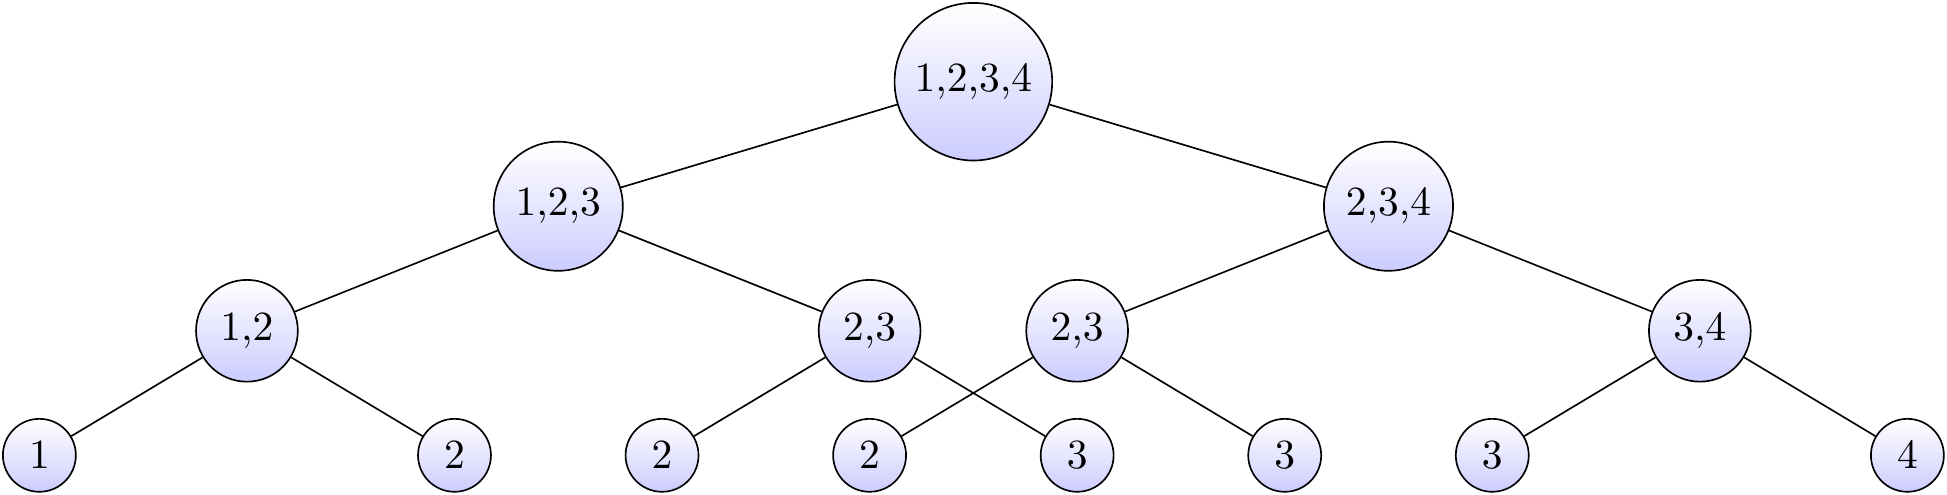
\includegraphics[width=0.9\linewidth]{tech-interview_files/figure-latex/unnamed-chunk-4-1} \caption{Some caption.}\label{fig:unnamed-chunk-4}
\end{figure}

\hypertarget{analysis-40}{%
\subsubsection{Analysis}\label{analysis-40}}

The time complexity is exponential, since there are some overlapping subproblems shown in the recursion tree.
\(O(2^{log(n)})\)

\hypertarget{algorithm-40}{%
\subsubsection{Algorithm}\label{algorithm-40}}

recursion \ref{recursion}

\hypertarget{java-code---recursion}{%
\subsection{Java Code - Recursion\}}\label{java-code---recursion}}

\begin{Shaded}
\begin{Highlighting}[]
\DataTypeTok{int} \FunctionTok{solution}\NormalTok{(}\DataTypeTok{int}\NormalTok{[] array) \{}
    \KeywordTok{return} \FunctionTok{rec}\NormalTok{(array, }\DecValTok{1}\NormalTok{);}
\NormalTok{\}}

\DataTypeTok{int} \FunctionTok{rec}\NormalTok{(}\DataTypeTok{int}\NormalTok{[] array, }\DataTypeTok{int}\NormalTok{ multiplier) \{}
    \DataTypeTok{int}\NormalTok{ len = array.}\FunctionTok{length}\NormalTok{;}

    \KeywordTok{if}\NormalTok{(len == }\DecValTok{1}\NormalTok{) \{}
        \KeywordTok{return}\NormalTok{ array[}\DecValTok{0}\NormalTok{] * multiplier;}
\NormalTok{    \}}

    \DataTypeTok{int}\NormalTok{ left = array[}\DecValTok{0}\NormalTok{] * multiplier + }\FunctionTok{rec}\NormalTok{(}\BuiltInTok{Arrays}\NormalTok{.}\FunctionTok{copyOfRange}\NormalTok{(array, }\DecValTok{1}\NormalTok{, len), multiplier + }\DecValTok{1}\NormalTok{);}
    \DataTypeTok{int}\NormalTok{ right = array[len - }\DecValTok{1}\NormalTok{] * multiplier + }\FunctionTok{rec}\NormalTok{(}\BuiltInTok{Arrays}\NormalTok{.}\FunctionTok{copyOfRange}\NormalTok{(array, }\DecValTok{0}\NormalTok{, len - }\DecValTok{1}\NormalTok{), multiplier + }\DecValTok{1}\NormalTok{);}

    \KeywordTok{return} \BuiltInTok{Math}\NormalTok{.}\FunctionTok{max}\NormalTok{(left, right);}
\NormalTok{\}}
\end{Highlighting}
\end{Shaded}

\hypertarget{solution---recursion-with-memoization}{%
\subsection{Solution - Recursion with Memoization\}}\label{solution---recursion-with-memoization}}

\hypertarget{walkthrough-38}{%
\subsubsection{Walkthrough}\label{walkthrough-38}}

We can derive \(multiplier = 1 + n - (j - i), 0 \le i < j \le n,\)

The sum of product array{[}i:j{]} is either computed directly (the base case), or it can be computed in constant time from
the already known sum of array{[}i+1:j{]} and array{[}i:j-1{]}.

\hypertarget{analysis-41}{%
\subsubsection{Analysis}\label{analysis-41}}

If we use dynamic programming and memorize all of these subresults, we will get an algorithm with \(O(n^2)\) time
complexity.

\hypertarget{algorithm-41}{%
\subsubsection{Algorithm}\label{algorithm-41}}

recursion \ref{recursion}, memoization \ref{memo}

\hypertarget{java-code---recursion-with-memoization}{%
\subsection{Java Code - Recursion with Memoization\}}\label{java-code---recursion-with-memoization}}

\begin{Shaded}
\begin{Highlighting}[]
\DataTypeTok{int} \FunctionTok{solution}\NormalTok{(}\DataTypeTok{int}\NormalTok{[] array) \{}
    \DataTypeTok{int}\NormalTok{ len = array.}\FunctionTok{length}\NormalTok{;}
    \DataTypeTok{int}\NormalTok{[][] dp = }\KeywordTok{new} \DataTypeTok{int}\NormalTok{[len + }\DecValTok{1}\NormalTok{][len + }\DecValTok{1}\NormalTok{];}

    \KeywordTok{return} \FunctionTok{memoization}\NormalTok{(array, }\DecValTok{0}\NormalTok{, len, dp);}
\NormalTok{\}}

\CommentTok{// 0 <= start < stop <= n}
\CommentTok{// start inclusive, stop exclusive}
\DataTypeTok{int} \FunctionTok{memoization}\NormalTok{(}\DataTypeTok{int}\NormalTok{[] array, }\DataTypeTok{int}\NormalTok{ start, }\DataTypeTok{int}\NormalTok{ stop, }\DataTypeTok{int}\NormalTok{[][] dp) \{}
    \DataTypeTok{int}\NormalTok{ multiplier = }\DecValTok{1}\NormalTok{ + array.}\FunctionTok{length}\NormalTok{ - (stop - start);}

    \KeywordTok{if}\NormalTok{(dp[start][stop] > }\DecValTok{0}\NormalTok{) \{}
        \CommentTok{//visited subproblem}
        \KeywordTok{return}\NormalTok{ dp[start][stop];}
\NormalTok{    \}}

    \KeywordTok{if}\NormalTok{(stop - start == }\DecValTok{1}\NormalTok{) \{}
        \KeywordTok{return}\NormalTok{ array[start] * multiplier;}
\NormalTok{    \}}

    \DataTypeTok{int}\NormalTok{ left = multiplier * array[start] + }\FunctionTok{memoization}\NormalTok{(array, start + }\DecValTok{1}\NormalTok{, stop, dp);}
    \DataTypeTok{int}\NormalTok{ right = multiplier * array[stop - }\DecValTok{1}\NormalTok{] + }\FunctionTok{memoization}\NormalTok{(array, start, stop - }\DecValTok{1}\NormalTok{, dp);}

    \DataTypeTok{int}\NormalTok{ result = }\BuiltInTok{Math}\NormalTok{.}\FunctionTok{max}\NormalTok{(left, right);}

\NormalTok{    dp[start][stop] = result;}

    \KeywordTok{return}\NormalTok{ result;}
\NormalTok{\}}
\end{Highlighting}
\end{Shaded}

\hypertarget{solution---dynamic-programming-with-tabulation}{%
\subsection{Solution - Dynamic Programming with Tabulation\}}\label{solution---dynamic-programming-with-tabulation}}

\hypertarget{walkthrough-39}{%
\subsubsection{Walkthrough}\label{walkthrough-39}}

We can derive \(multiplier = 1 + n - (j - i), 0 \le i < j \le n,\)

As an alternative, we can use tabulation and start by filling up the memo table. Note that the order of computation
matters: to compute the value memo{[}i{]}{[}j{]}, the values of memo{[}i+1{]}{[}j{]} and memo{[}i{]}{[}j-1{]} must first be known.

Here is the final view of table from the example:

\begin{verbatim}
0   4   11  20  30
0   0   8   18  29
0   0   0   12  25
0   0   0   0   16
0   0   0   0   0
\end{verbatim}

\hypertarget{analysis-42}{%
\subsubsection{Analysis}\label{analysis-42}}

\hypertarget{algorithm-42}{%
\subsubsection{Algorithm}\label{algorithm-42}}

dp \ref{dp}, tabulation \ref{table}

\hypertarget{java-code---dynamic-programming-with-tabulation}{%
\subsection{Java Code - Dynamic Programming with Tabulation\}}\label{java-code---dynamic-programming-with-tabulation}}

\begin{verbatim}
int solution(int[] array) {
    int len = array.length;
    int[][] dp = new int[len + 1][len + 1];

    return tabulation(array, dp, len);
}

int tabulation(int[] array, int[][] dp, int len) {
    for(int i = 0; i < len; i++) {
        dp[i][i + 1] = len * array[i];
    }

    for (int i = len - 1; i >= 0; i--) {
        for(int j = i + 2; j <= len; j++) {
            int multiplier = 1 + len - (j - i);
            int left = multiplier * array[i] + dp[i + 1][j];
            int right = multiplier * array[j - 1] + dp[i][j - 1];
            int result = Math.max(left, right);
            dp[i][j] = result;
        }
    }

    return dp[0][len];
}
\end{verbatim}

\hypertarget{shortest-word-distance}{%
\section{Shortest Word Distance / / \}}\label{shortest-word-distance}}

\hypertarget{description-39}{%
\subsection{Description}\label{description-39}}

Given a list of words and two words word1 and word2, return the shortest distance between these two words in the list.

\hypertarget{example-38}{%
\subsection{Example}\label{example-38}}

words = {[}``practice'', ``makes'', ``perfect'', ``coding'', ``makes''{]}

word1 = ``coding'', word2=``practice'' result is 3

word1 = ``makes'', word2=``coding'' result is 1

\hypertarget{solution-31}{%
\subsection{Solution}\label{solution-31}}

\hypertarget{walkthrough-40}{%
\subsubsection{Walkthrough}\label{walkthrough-40}}

Record the indices for each word. Retrieve the minimum distance between two group of indices.

\hypertarget{analysis-43}{%
\subsubsection{Analysis}\label{analysis-43}}

Each word in the list is visited once, and each index in both list is visited once. Thus time complexity is O(n),
where the Auxiliary Space is O(n) for storing indices.

\hypertarget{algorithm-43}{%
\subsubsection{Algorithm}\label{algorithm-43}}

\hypertarget{java-code-34}{%
\subsection{Java Code}\label{java-code-34}}

\begin{Shaded}
\begin{Highlighting}[]
\KeywordTok{public} \DataTypeTok{int} \FunctionTok{shortestDistance}\NormalTok{(}\BuiltInTok{String}\NormalTok{[] words, }\BuiltInTok{String}\NormalTok{ word1, }\BuiltInTok{String}\NormalTok{ word2) \{}
    \CommentTok{// list of indices for word1 and word2 in the array respectively.}
    \BuiltInTok{List}\NormalTok{<}\BuiltInTok{Integer}\NormalTok{> list1 = }\KeywordTok{new} \BuiltInTok{ArrayList}\NormalTok{<>();}
    \BuiltInTok{List}\NormalTok{<}\BuiltInTok{Integer}\NormalTok{> list2 = }\KeywordTok{new} \BuiltInTok{ArrayList}\NormalTok{<>();}

    \KeywordTok{for}\NormalTok{(}\DataTypeTok{int}\NormalTok{ i = }\DecValTok{0}\NormalTok{; i < words.}\FunctionTok{length}\NormalTok{; i++) \{}
        \KeywordTok{if}\NormalTok{(words[i].}\FunctionTok{equals}\NormalTok{(word1)) \{}
\NormalTok{            list1.}\FunctionTok{add}\NormalTok{(i);}
\NormalTok{        \} }\KeywordTok{else} \KeywordTok{if}\NormalTok{(words[i].}\FunctionTok{equals}\NormalTok{(word2)) \{}
\NormalTok{            list2.}\FunctionTok{add}\NormalTok{(i);}
\NormalTok{        \}}
\NormalTok{    \}}

    \DataTypeTok{int}\NormalTok{ min = words.}\FunctionTok{length}\NormalTok{;}
    \KeywordTok{for}\NormalTok{(}\DataTypeTok{int}\NormalTok{ i = }\DecValTok{0}\NormalTok{, j = }\DecValTok{0}\NormalTok{; i < list1.}\FunctionTok{size}\NormalTok{() && j < list2.}\FunctionTok{size}\NormalTok{();) \{}
        \DataTypeTok{int}\NormalTok{ index1 = list1.}\FunctionTok{get}\NormalTok{(i);}
        \DataTypeTok{int}\NormalTok{ index2 = list2.}\FunctionTok{get}\NormalTok{(i);}

\NormalTok{        min = }\BuiltInTok{Math}\NormalTok{.}\FunctionTok{min}\NormalTok{(min, }\BuiltInTok{Math}\NormalTok{.}\FunctionTok{abs}\NormalTok{(index1 - index2));}

        \KeywordTok{if}\NormalTok{(index1 < index2) \{}
\NormalTok{            i++;}
\NormalTok{        \} }\KeywordTok{else} \KeywordTok{if}\NormalTok{(index1 > index2) \{}
\NormalTok{            j++;}
\NormalTok{        \} }\KeywordTok{else}\NormalTok{ \{}
            \CommentTok{// comparing the same indices}
            \KeywordTok{return} \DecValTok{0}\NormalTok{;}
\NormalTok{        \}}
\NormalTok{    \}}

    \KeywordTok{return}\NormalTok{ min;}
\NormalTok{\}}
\end{Highlighting}
\end{Shaded}

\hypertarget{matrix}{%
\chapter{Matrix}\label{matrix}}

\hypertarget{design-a-tic-tac-toe-leetcode-348-medium}{%
\section{Design a Tic-tac-toe / LeetCode 348 / Medium\}}\label{design-a-tic-tac-toe-leetcode-348-medium}}

\hypertarget{description-40}{%
\subsection{Description\}}\label{description-40}}

Design a Tic-tac-toe game that is played between two players on a n x n grid.

\hypertarget{example-39}{%
\subsection{Example\}}\label{example-39}}

\hypertarget{solution-32}{%
\subsection{Solution\}}\label{solution-32}}

\hypertarget{walkthrough-41}{%
\subsubsection{Walkthrough\}\textbackslash{}}\label{walkthrough-41}}

Check if the player win for the same row, column, forward and back diagonals.

\hypertarget{analysis-44}{%
\subsubsection{Analysis\}\textbackslash{}}\label{analysis-44}}

All entries in matrix will be visited, that is, O(rows * cols)

\hypertarget{algorithm-44}{%
\subsubsection{Algorithm\}\textbackslash{}}\label{algorithm-44}}

\hypertarget{java-code-35}{%
\subsection{Java Code\}}\label{java-code-35}}

\begin{Shaded}
\begin{Highlighting}[]
\DataTypeTok{int}\NormalTok{[][] matrix;}

\KeywordTok{public} \DataTypeTok{int} \FunctionTok{move}\NormalTok{(}\DataTypeTok{int}\NormalTok{ row, }\DataTypeTok{int}\NormalTok{ col, }\DataTypeTok{int}\NormalTok{ player) \{}
\NormalTok{    matrix[row][col]=player;}

    \CommentTok{//check row}
    \DataTypeTok{boolean}\NormalTok{ win = }\KeywordTok{true}\NormalTok{;}
    \KeywordTok{for}\NormalTok{(}\DataTypeTok{int}\NormalTok{ i = }\DecValTok{0}\NormalTok{; i < matrix.}\FunctionTok{length}\NormalTok{; i++)\{}
        \KeywordTok{if}\NormalTok{(matrix[row][i] != player)\{}
\NormalTok{            win = }\KeywordTok{false}\NormalTok{;}
            \KeywordTok{break}\NormalTok{;}
\NormalTok{        \}}
\NormalTok{    \}}

    \KeywordTok{if}\NormalTok{(win) }\KeywordTok{return}\NormalTok{ player;}

    \CommentTok{//check column}
\NormalTok{    win = }\KeywordTok{true}\NormalTok{;}
    \KeywordTok{for}\NormalTok{(}\DataTypeTok{int}\NormalTok{ i = }\DecValTok{0}\NormalTok{; i < matrix.}\FunctionTok{length}\NormalTok{; i++)\{}
        \KeywordTok{if}\NormalTok{(matrix[i][col] != player)\{}
\NormalTok{            win = }\KeywordTok{false}\NormalTok{;}
            \KeywordTok{break}\NormalTok{;}
\NormalTok{        \}}
\NormalTok{    \}}

    \KeywordTok{if}\NormalTok{(win) }\KeywordTok{return}\NormalTok{ player;}

    \CommentTok{//check back diagonal}
\NormalTok{    win = }\KeywordTok{true}\NormalTok{;}
    \KeywordTok{for}\NormalTok{(}\DataTypeTok{int}\NormalTok{ i = }\DecValTok{0}\NormalTok{; i < matrix.}\FunctionTok{length}\NormalTok{; i++)\{}
        \KeywordTok{if}\NormalTok{(matrix[i][i] != player)\{}
\NormalTok{            win = }\KeywordTok{false}\NormalTok{;}
            \KeywordTok{break}\NormalTok{;}
\NormalTok{        \}}
\NormalTok{    \}}

    \KeywordTok{if}\NormalTok{(win) }\KeywordTok{return}\NormalTok{ player;}

    \CommentTok{//check forward diagonal}
\NormalTok{    win = }\KeywordTok{true}\NormalTok{;}
    \KeywordTok{for}\NormalTok{(}\DataTypeTok{int}\NormalTok{ i = }\DecValTok{0}\NormalTok{; i < matrix.}\FunctionTok{length}\NormalTok{; i++)\{}
        \KeywordTok{if}\NormalTok{(matrix[i][matrix.}\FunctionTok{length}\NormalTok{-i}\DecValTok{-1}\NormalTok{] != player)\{}
\NormalTok{            win = }\KeywordTok{false}\NormalTok{;}
            \KeywordTok{break}\NormalTok{;}
\NormalTok{        \}}
\NormalTok{    \}}

    \KeywordTok{if}\NormalTok{(win) }\KeywordTok{return}\NormalTok{ player;}

    \KeywordTok{return} \DecValTok{0}\NormalTok{;}
\NormalTok{\}}
\end{Highlighting}
\end{Shaded}

\hypertarget{rotate-image-leet-code-48-medium}{%
\section{Rotate Image / Leet Code 48 / Medium\}}\label{rotate-image-leet-code-48-medium}}

\hypertarget{description-41}{%
\subsection{Description\}}\label{description-41}}

You are given an n x n 2D matrix representing an image. Rotate the image by 90 degrees (clockwise). You have
to rotate the image in-place, which means you have to modify the input 2D matrix directly. DO NOT allocate
another 2D matrix and do the rotation.

\hypertarget{example-40}{%
\subsection{Example\}}\label{example-40}}

Given input matrix, and rotate the input matrix in-place.

\begin{verbatim}
[1,2,3],          [7,4,1],
[4,5,6],  ==>     [8,5,2],
[7,8,9]           [9,6,3]
\end{verbatim}

\hypertarget{solution-33}{%
\subsection{Solution\}}\label{solution-33}}

\hypertarget{walkthrough-42}{%
\subsubsection{Walkthrough\}\textbackslash{}}\label{walkthrough-42}}

Take this matrix as example,

\begin{verbatim}
[1,2,3],
[4,5,6],
[7,8,9]
\end{verbatim}

first swap the symmetric elements via top-left to bottom-right diagnal,

\begin{verbatim}
[1,4,7],
[2,5,8],
[3,6,9]
\end{verbatim}

and swap columns via centeral vertical line.

\begin{verbatim}
[7,|4|,1],
[8,|5|,2],
[9,|6|,3]
\end{verbatim}

\hypertarget{analysis-45}{%
\subsubsection{Analysis\}\textbackslash{}}\label{analysis-45}}

Time complexity is \(O(n^2)\) as there are two loops

\hypertarget{algorithm-45}{%
\subsubsection{Algorithm\}\textbackslash{}}\label{algorithm-45}}

\hypertarget{java-code-36}{%
\subsection{Java Code\}}\label{java-code-36}}

\begin{Shaded}
\begin{Highlighting}[]
\KeywordTok{public} \DataTypeTok{void} \FunctionTok{rotate}\NormalTok{(}\DataTypeTok{int}\NormalTok{[][] matrix) \{}
    \CommentTok{//Swap symmetric element via diagnal}
    \KeywordTok{for}\NormalTok{ (}\DataTypeTok{int}\NormalTok{ i = }\DecValTok{0}\NormalTok{; i <  matrix.}\FunctionTok{length}\NormalTok{; i++) \{}
        \KeywordTok{for}\NormalTok{ (}\DataTypeTok{int}\NormalTok{ j = }\DecValTok{0}\NormalTok{; j < i; j++) \{}
            \DataTypeTok{int}\NormalTok{ temp = matrix[i][j];}
\NormalTok{            matrix[i][j] = matrix[j][i];}
\NormalTok{            matrix[j][i] = temp;}
\NormalTok{        \}}
\NormalTok{    \}}
    \CommentTok{//Swap columns via centeral vertical line}
    \KeywordTok{for}\NormalTok{ (}\DataTypeTok{int}\NormalTok{ i = }\DecValTok{0}\NormalTok{, j = matrix.}\FunctionTok{length}\NormalTok{ - }\DecValTok{1}\NormalTok{; i < matrix.}\FunctionTok{length}\NormalTok{ / }\DecValTok{2}\NormalTok{; i++, j--) \{}
        \KeywordTok{for}\NormalTok{ (}\DataTypeTok{int}\NormalTok{ k = }\DecValTok{0}\NormalTok{; k < matrix.}\FunctionTok{length}\NormalTok{; k++) \{}
            \DataTypeTok{int}\NormalTok{ temp = matrix[k][i];}
\NormalTok{            matrix[k][i] = matrix[k][j];}
\NormalTok{            matrix[k][j] = temp;}
\NormalTok{        \}}
\NormalTok{    \}}
\NormalTok{\}}
\end{Highlighting}
\end{Shaded}

\hypertarget{spiral-matrix-leetcode-54-medium}{%
\section{Spiral Matrix / LeetCode 54 / Medium\}}\label{spiral-matrix-leetcode-54-medium}}

\hypertarget{description-42}{%
\subsection{Description\}}\label{description-42}}

Given a matrix of m x n elements (m rows, n columns), return all elements of the matrix in spiral order.

\hypertarget{example-41}{%
\subsection{Example\}}\label{example-41}}

Input:

\begin{Shaded}
\begin{Highlighting}[]
\DecValTok{1}\NormalTok{, }\DecValTok{2}\NormalTok{, }\DecValTok{3}\NormalTok{ ,}
\DecValTok{4}\NormalTok{, }\DecValTok{5}\NormalTok{, }\DecValTok{6}\NormalTok{ ,}
\DecValTok{7}\NormalTok{, }\DecValTok{8}\NormalTok{, }\DecValTok{9}
\end{Highlighting}
\end{Shaded}

Output: {[}1,2,3,6,9,8,7,4,5{]}

Input:

\begin{Shaded}
\begin{Highlighting}[]
\DecValTok{1}\NormalTok{, }\DecValTok{2}\NormalTok{, }\DecValTok{3}\NormalTok{, }\DecValTok{4}\NormalTok{,}
\DecValTok{5}\NormalTok{, }\DecValTok{6}\NormalTok{, }\DecValTok{7}\NormalTok{, }\DecValTok{8}\NormalTok{,}
\DecValTok{9}\NormalTok{,}\DecValTok{10}\NormalTok{,}\DecValTok{11}\NormalTok{,}\DecValTok{12}
\end{Highlighting}
\end{Shaded}

Output: {[}1,2,3,4,8,12,11,10,9,5,6,7{]}
\#\#\# Solution\}
\#\#\#\# Walkthrough\}\textbackslash{}
While walking through the circles, track current left, right, top, and bottom positions.

\begin{Shaded}
\begin{Highlighting}[]
\NormalTok{(r)}
    \DecValTok{0}  \DecValTok{1}  \DecValTok{2}\NormalTok{   (c)}
 \DecValTok{0}\NormalTok{  -  -  -}
 \DecValTok{1}\NormalTok{  |  >  |}
 \DecValTok{2}\NormalTok{  -  -  |}
\end{Highlighting}
\end{Shaded}

\begin{verbatim}
\*  Going rightward
\*  Going downward
\*  Going leftward
\*  Going upward
\end{verbatim}

Be sure to check for duplicated column or row before going for each direction.

\hypertarget{analysis-46}{%
\subsubsection{Analysis\}\textbackslash{}}\label{analysis-46}}

Time complexity is O(rows * cols), since all elements are visited once

\hypertarget{algorithm-46}{%
\subsubsection{Algorithm\}\textbackslash{}}\label{algorithm-46}}

\hypertarget{java-code-37}{%
\subsection{Java Code\}}\label{java-code-37}}

\begin{Shaded}
\begin{Highlighting}[]
\KeywordTok{public} \BuiltInTok{List} \FunctionTok{spiralOrder}\NormalTok{(}\DataTypeTok{int}\NormalTok{[][] matrix) \{}
    \BuiltInTok{List}\NormalTok{ result = }\KeywordTok{new} \BuiltInTok{ArrayList}\NormalTok{<>();}

    \KeywordTok{if}\NormalTok{(matrix.}\FunctionTok{length}\NormalTok{ == }\DecValTok{0}\NormalTok{) \{}
        \KeywordTok{return}\NormalTok{ result;}
\NormalTok{    \}}

    \DataTypeTok{int}\NormalTok{ rows = matrix.}\FunctionTok{length}\NormalTok{;}
    \DataTypeTok{int}\NormalTok{ cols = matrix[}\DecValTok{0}\NormalTok{].}\FunctionTok{length}\NormalTok{;}

    \CommentTok{// position of left, right, top and buttom border}
    \DataTypeTok{int}\NormalTok{ left = }\DecValTok{0}\NormalTok{;}
    \DataTypeTok{int}\NormalTok{ right = cols - }\DecValTok{1}\NormalTok{;}
    \DataTypeTok{int}\NormalTok{ top = }\DecValTok{0}\NormalTok{;}
    \DataTypeTok{int}\NormalTok{ bottom = rows - }\DecValTok{1}\NormalTok{;}

    \KeywordTok{while}\NormalTok{( result.}\FunctionTok{size}\NormalTok{() < (cols * rows) ) \{}
        \CommentTok{//traverse a circle}

        \CommentTok{// avoid duplicated row}
        \KeywordTok{if}\NormalTok{(top > bottom) \{}
            \KeywordTok{break}\NormalTok{;}
\NormalTok{        \}}

        \CommentTok{//going rightward}
        \KeywordTok{for}\NormalTok{(}\DataTypeTok{int}\NormalTok{ i = left; i <= right; i++)\{}
\NormalTok{            result.}\FunctionTok{add}\NormalTok{(matrix[top][i]);}
\NormalTok{        \}}
\NormalTok{        top++;}

        \CommentTok{// avoid duplicated column}
        \KeywordTok{if}\NormalTok{(left > right) \{}
            \KeywordTok{break}\NormalTok{;}
\NormalTok{        \}}

        \CommentTok{//going downward}
        \KeywordTok{for}\NormalTok{(}\DataTypeTok{int}\NormalTok{ i = top; i <= bottom; i++)\{}
\NormalTok{            result.}\FunctionTok{add}\NormalTok{(matrix[i][right]);}
\NormalTok{        \}}
\NormalTok{        right--;}

        \CommentTok{// avoid duplicated row}
        \KeywordTok{if}\NormalTok{(top > bottom) \{}
            \KeywordTok{break}\NormalTok{;}
\NormalTok{        \}}

        \CommentTok{// going leftward}
        \KeywordTok{for}\NormalTok{(}\DataTypeTok{int}\NormalTok{ i = right; i >= left; i--)\{}
\NormalTok{            result.}\FunctionTok{add}\NormalTok{(matrix[bottom][i]);}
\NormalTok{        \}}
\NormalTok{        bottom--;}

        \CommentTok{// avoid duplicated column}
        \KeywordTok{if}\NormalTok{(left > right) \{}
            \KeywordTok{break}\NormalTok{;}
\NormalTok{        \}}

        \CommentTok{// going upward}
        \KeywordTok{for}\NormalTok{(}\DataTypeTok{int}\NormalTok{ i = bottom; i >= top; i--)\{}
\NormalTok{            result.}\FunctionTok{add}\NormalTok{(matrix[i][left]);}
\NormalTok{        \}}
\NormalTok{        left++;}
\NormalTok{    \}}

    \KeywordTok{return}\NormalTok{ result;}
\NormalTok{\}}
\end{Highlighting}
\end{Shaded}

\hypertarget{search-a-2d-matrix-leetcode-74-medium}{%
\section{Search a 2D Matrix / LeetCode 74 / Medium\}}\label{search-a-2d-matrix-leetcode-74-medium}}

\hypertarget{description-43}{%
\subsection{Description\}}\label{description-43}}

Write an efficient algorithm that searches for a value in an m x n matrix. This matrix has the following properties:

\begin{verbatim}
\*  Integers in each row are sorted from left to right.
\*  The first integer of each row is greater than the last integer of the previous row.
\end{verbatim}

\hypertarget{example-42}{%
\subsection{Example\}}\label{example-42}}

Input:

\begin{Shaded}
\begin{Highlighting}[]
\NormalTok{[}\DecValTok{1}\NormalTok{,   }\DecValTok{3}\NormalTok{,  }\DecValTok{5}\NormalTok{,  }\DecValTok{7}\NormalTok{],}
\NormalTok{[}\DecValTok{10}\NormalTok{, }\DecValTok{11}\NormalTok{, }\DecValTok{16}\NormalTok{, }\DecValTok{20}\NormalTok{],}
\NormalTok{[}\DecValTok{23}\NormalTok{, }\DecValTok{30}\NormalTok{, }\DecValTok{34}\NormalTok{, }\DecValTok{50}\NormalTok{]}
\end{Highlighting}
\end{Shaded}

target = 3
Output: true

Input:

\begin{Shaded}
\begin{Highlighting}[]
\NormalTok{[}\DecValTok{1}\NormalTok{,   }\DecValTok{3}\NormalTok{,  }\DecValTok{5}\NormalTok{,  }\DecValTok{7}\NormalTok{],}
\NormalTok{[}\DecValTok{10}\NormalTok{, }\DecValTok{11}\NormalTok{, }\DecValTok{16}\NormalTok{, }\DecValTok{20}\NormalTok{],}
\NormalTok{[}\DecValTok{23}\NormalTok{, }\DecValTok{30}\NormalTok{, }\DecValTok{34}\NormalTok{, }\DecValTok{50}\NormalTok{]}
\end{Highlighting}
\end{Shaded}

target = 13
Output: false
\#\#\# Solution\}
\#\#\#\# Walkthrough\}\textbackslash{}
We can treat the 2D matrix as the one large array, and search the element using binary search. We only need to compute
middle of row or column for each divide-and-conquer turn.

\hypertarget{analysis-47}{%
\subsubsection{Analysis\}\textbackslash{}}\label{analysis-47}}

The overall time complexity is O(log(rows * cols))

\hypertarget{algorithm-47}{%
\subsubsection{Algorithm\}\textbackslash{}}\label{algorithm-47}}

recursion \ref{dnc}

\hypertarget{java-code-38}{%
\subsection{Java Code\}}\label{java-code-38}}

\begin{Shaded}
\begin{Highlighting}[]
\KeywordTok{public} \DataTypeTok{boolean} \FunctionTok{searchMatrix}\NormalTok{(}\DataTypeTok{int}\NormalTok{[][] matrix, }\DataTypeTok{int}\NormalTok{ target) \{}
    \KeywordTok{if}\NormalTok{(matrix == }\KeywordTok{null}\NormalTok{ || matrix.}\FunctionTok{length}\NormalTok{ == }\DecValTok{0}\NormalTok{ || matrix[}\DecValTok{0}\NormalTok{].}\FunctionTok{length}\NormalTok{ == }\DecValTok{0}\NormalTok{) \{}
        \KeywordTok{return} \KeywordTok{false}\NormalTok{;}
\NormalTok{    \}}

    \DataTypeTok{int}\NormalTok{ rows = matrix.}\FunctionTok{length}\NormalTok{;}
    \DataTypeTok{int}\NormalTok{ cols = matrix[}\DecValTok{0}\NormalTok{].}\FunctionTok{length}\NormalTok{;}

    \DataTypeTok{int}\NormalTok{ start = }\DecValTok{0}\NormalTok{;}
    \DataTypeTok{int}\NormalTok{ end = rows * cols - }\DecValTok{1}\NormalTok{;}

    \KeywordTok{while}\NormalTok{(start <= end) \{}
        \DataTypeTok{int}\NormalTok{ mid = (end - start) / }\DecValTok{2}\NormalTok{ + start;}
        \DataTypeTok{int}\NormalTok{ midRow = mid / cols;}
        \DataTypeTok{int}\NormalTok{ midCol = mid % cols;}

        \KeywordTok{if}\NormalTok{(matrix[midRow][midCol] == target) \{}
            \KeywordTok{return} \KeywordTok{true}\NormalTok{;}
\NormalTok{        \} }\KeywordTok{else} \KeywordTok{if}\NormalTok{(matrix[midRow][midCol] < target) \{}
\NormalTok{            start = mid + }\DecValTok{1}\NormalTok{;}
\NormalTok{        \} }\KeywordTok{else}\NormalTok{ \{}
            \CommentTok{//matrix[midRow][midCol] > target}
\NormalTok{            end = mid - }\DecValTok{1}\NormalTok{;}
\NormalTok{        \}}
\NormalTok{    \}}

    \KeywordTok{return} \KeywordTok{false}\NormalTok{;}
\NormalTok{\}}
\end{Highlighting}
\end{Shaded}

\hypertarget{search-a-2d-matrix-ii-leetcode-240-medium}{%
\section{Search a 2D Matrix II / LeetCode 240 / Medium\}}\label{search-a-2d-matrix-ii-leetcode-240-medium}}

\hypertarget{description-44}{%
\subsection{Description\}}\label{description-44}}

Write an efficient algorithm that searches for a value in an m x n matrix. This matrix has the following properties:

\begin{verbatim}
\*  Integers in each row are sorted in ascending from left to right.
\*  Integers in each column are sorted in ascending from top to bottom.
\end{verbatim}

\hypertarget{example-43}{%
\subsection{Example\}}\label{example-43}}

\texttt{java\ {[}\ {[}1,\ \ \ 4,\ \ 7,\ 11,\ 15{]},\ {[}2,\ \ \ 5,\ \ 8,\ 12,\ 19{]},\ {[}3,\ \ \ 6,\ \ 9,\ 16,\ 22{]},\ {[}10,\ 13,\ 14,\ 17,\ 24{]},\ {[}18,\ 21,\ 23,\ 26,\ 30{]}\ {]}}, 5 returns true

\hypertarget{solution-34}{%
\subsection{Solution\}}\label{solution-34}}

\hypertarget{walkthrough-43}{%
\subsubsection{Walkthrough\}\textbackslash{}}\label{walkthrough-43}}

Traverse the matrix by

\begin{verbatim}
\*  locate row when target is smaller than m[r][c]
\*  locate col when target is larger than m[r][c]
\end{verbatim}

\hypertarget{analysis-48}{%
\subsubsection{Analysis\}\textbackslash{}}\label{analysis-48}}

A portion of cell is visited, O(m + n) - instead of every cell (m * n)

\hypertarget{algorithm-48}{%
\subsubsection{Algorithm\}\textbackslash{}}\label{algorithm-48}}

\hypertarget{java-code-39}{%
\subsection{Java Code\}}\label{java-code-39}}

\begin{Shaded}
\begin{Highlighting}[]
\KeywordTok{public} \DataTypeTok{boolean} \FunctionTok{searchMatrix}\NormalTok{(}\DataTypeTok{int}\NormalTok{[][] matrix, }\DataTypeTok{int}\NormalTok{ target) \{}
    \KeywordTok{if}\NormalTok{(matrix == }\KeywordTok{null}\NormalTok{ || matrix.}\FunctionTok{length}\NormalTok{ == }\DecValTok{0}\NormalTok{) \{}
        \KeywordTok{return} \KeywordTok{false}\NormalTok{;}
\NormalTok{    \}}

    \DataTypeTok{int}\NormalTok{ rows = matrix.}\FunctionTok{length}\DecValTok{-1}\NormalTok{;}
    \DataTypeTok{int}\NormalTok{ cols = matrix[}\DecValTok{0}\NormalTok{].}\FunctionTok{length}\DecValTok{-1}\NormalTok{;}

    \DataTypeTok{int}\NormalTok{ r = rows;}
    \DataTypeTok{int}\NormalTok{ c = }\DecValTok{0}\NormalTok{;}

    \KeywordTok{while}\NormalTok{(r >= }\DecValTok{0}\NormalTok{ && c <= cols)\{}
        \KeywordTok{if}\NormalTok{(target < matrix[r][c]) \{}
\NormalTok{            r--;}
\NormalTok{        \} }\KeywordTok{else} \KeywordTok{if}\NormalTok{(target > matrix[r][c]) \{}
\NormalTok{            c++;}
\NormalTok{        \} }\KeywordTok{else}\NormalTok{ \{}
            \KeywordTok{return} \KeywordTok{true}\NormalTok{;}
\NormalTok{        \}}
\NormalTok{    \}}

    \KeywordTok{return} \KeywordTok{false}\NormalTok{;}
\NormalTok{\}}
\end{Highlighting}
\end{Shaded}

\hypertarget{minimum-path-sum-leetcode-64-medium}{%
\section{Minimum Path Sum / LeetCode 64 / Medium\}}\label{minimum-path-sum-leetcode-64-medium}}

\hypertarget{description-45}{%
\subsection{Description\}}\label{description-45}}

Given a m x n grid filled with non-negative numbers, find a path from top left to bottom right which minimizes the sum
of all numbers along its path. You can only move either down or right at any point in time.
\#\#\# Example\}
Input:

\begin{Shaded}
\begin{Highlighting}[]
\NormalTok{[}\DecValTok{1}\NormalTok{],[}\DecValTok{3}\NormalTok{],[}\DecValTok{1}\NormalTok{],}
 \DecValTok{1}\NormalTok{,  }\DecValTok{5}\NormalTok{, [}\DecValTok{1}\NormalTok{],}
 \DecValTok{4}\NormalTok{,  }\DecValTok{2}\NormalTok{, [}\DecValTok{1}\NormalTok{]}
\end{Highlighting}
\end{Shaded}

Output: 7, because the path \(1 -> 3 -> 1 -> 1 -> 1\) minimizes the sum.

\hypertarget{solution---recursive}{%
\subsection{Solution - Recursive\}}\label{solution---recursive}}

\hypertarget{walkthrough-44}{%
\subsubsection{Walkthrough\}\textbackslash{}}\label{walkthrough-44}}

Time Complexity is exponential.

\begin{figure}
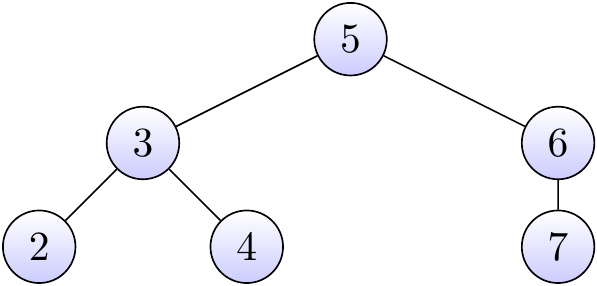
\includegraphics[width=0.9\linewidth]{tech-interview_files/figure-latex/unnamed-chunk-5-1} \caption{Some caption.}\label{fig:unnamed-chunk-5}
\end{figure}

See the above recursion tree, there are many nodes which apear more than once.
Final cost matrix:

\begin{Shaded}
\begin{Highlighting}[]
\NormalTok{[}\DecValTok{1}\NormalTok{], [}\DecValTok{4}\NormalTok{], [}\DecValTok{5}\NormalTok{]}
\DecValTok{2}\NormalTok{,   }\DecValTok{7}\NormalTok{,   [}\DecValTok{6}\NormalTok{]}
\DecValTok{6}\NormalTok{,   }\DecValTok{8}\NormalTok{,   [}\DecValTok{7}\NormalTok{]}
\end{Highlighting}
\end{Shaded}

\hypertarget{analysis-49}{%
\subsubsection{Analysis\}\textbackslash{}}\label{analysis-49}}

There will be \(2^{h + 1} - 1 = 2^{log(m*n) + 1} - 1\) subproblems, including the overlapping subproblems, which means
the same subproblem has been computed again and gain. Thus, the time complexity is \(O(2^{log(m * n)})\)

\hypertarget{algorithm-49}{%
\subsubsection{Algorithm\}\textbackslash{}}\label{algorithm-49}}

recursive \ref{recursive}

\hypertarget{java-code---recursive}{%
\subsection{Java Code - Recursive\}}\label{java-code---recursive}}

\begin{Shaded}
\begin{Highlighting}[]
\KeywordTok{public} \DataTypeTok{int} \FunctionTok{minPathSum}\NormalTok{(}\DataTypeTok{int}\NormalTok{[][] grid) \{}
    \KeywordTok{if}\NormalTok{(grid == }\KeywordTok{null}\NormalTok{ || grid.}\FunctionTok{length}\NormalTok{==}\DecValTok{0}\NormalTok{) \{}
        \KeywordTok{return} \DecValTok{0}\NormalTok{;}
\NormalTok{    \}}

    \KeywordTok{return} \FunctionTok{rec}\NormalTok{(}\DecValTok{0}\NormalTok{,}\DecValTok{0}\NormalTok{,grid);}
\NormalTok{\}}

\KeywordTok{public} \DataTypeTok{int} \FunctionTok{rec}\NormalTok{(}\DataTypeTok{int}\NormalTok{ i, }\DataTypeTok{int}\NormalTok{ j, }\DataTypeTok{int}\NormalTok{[][] grid)\{}
    \DataTypeTok{int}\NormalTok{ rows = grid.}\FunctionTok{length}\NormalTok{;}
    \DataTypeTok{int}\NormalTok{ cols = grid[}\DecValTok{0}\NormalTok{].}\FunctionTok{length}\NormalTok{;}


    \KeywordTok{if}\NormalTok{(i == (rows - }\DecValTok{1}\NormalTok{) && j == (cols - }\DecValTok{1}\NormalTok{))\{}
        \CommentTok{//at bottom right}
        \KeywordTok{return}\NormalTok{ grid[i][j];}
\NormalTok{    \} }\KeywordTok{else} \KeywordTok{if}\NormalTok{(i < (rows - }\DecValTok{1}\NormalTok{) && j == (cols - }\DecValTok{1}\NormalTok{)) \{}
        \CommentTok{//at last column, moving downward}
        \KeywordTok{return}\NormalTok{ grid[i][j] + }\FunctionTok{dfs}\NormalTok{(i+}\DecValTok{1}\NormalTok{, j, grid);}
\NormalTok{    \} }\KeywordTok{else} \KeywordTok{if}\NormalTok{(i == (rows - }\DecValTok{1}\NormalTok{) && j < (cols - }\DecValTok{1}\NormalTok{)) \{}
        \CommentTok{//at last row, moving rightward}
        \KeywordTok{return}\NormalTok{ grid[i][j] + }\FunctionTok{dfs}\NormalTok{(i, j+}\DecValTok{1}\NormalTok{, grid);}
\NormalTok{    \} }\KeywordTok{else}\NormalTok{ \{}
        \CommentTok{//other place, get min of downward and rightward}
        \DataTypeTok{int}\NormalTok{ r1 = grid[i][j] + }\FunctionTok{rec}\NormalTok{(i+}\DecValTok{1}\NormalTok{, j, grid);}
        \DataTypeTok{int}\NormalTok{ r2 = grid[i][j] + }\FunctionTok{rec}\NormalTok{(i, j+}\DecValTok{1}\NormalTok{, grid);}
        \KeywordTok{return} \BuiltInTok{Math}\NormalTok{.}\FunctionTok{min}\NormalTok{(r1,r2);}
\NormalTok{    \}}
\NormalTok{\}}
\end{Highlighting}
\end{Shaded}

\hypertarget{solution---dynamic-programming}{%
\subsection{Solution - Dynamic Programming\}}\label{solution---dynamic-programming}}

\hypertarget{walkthrough-45}{%
\subsubsection{Walkthrough\}\textbackslash{}}\label{walkthrough-45}}

\begin{verbatim}
\*  create a cost matrix of the same size
\*  init cost[0][0] to be grid[0][0]
\*  init first row and first column, previous cell cost plus current cell cost
\*  For each other cell, determine the minimum cost of previous top or left cell plus current cell cost.
\end{verbatim}

\hypertarget{analysis-50}{%
\subsubsection{Analysis\}\textbackslash{}}\label{analysis-50}}

Complexity: O(n * m) since each cell is visited once

\hypertarget{algorithm-50}{%
\subsubsection{Algorithm\}\textbackslash{}}\label{algorithm-50}}

dp \ref{dp}

\hypertarget{java-code---dynamic-programming}{%
\subsection{Java Code - Dynamic Programming\}}\label{java-code---dynamic-programming}}

\begin{Shaded}
\begin{Highlighting}[]
\KeywordTok{public} \DataTypeTok{int} \FunctionTok{minPathSum}\NormalTok{(}\DataTypeTok{int}\NormalTok{[][] grid) \{}
    \KeywordTok{if}\NormalTok{(grid == }\KeywordTok{null}\NormalTok{ || grid.}\FunctionTok{length}\NormalTok{ == }\DecValTok{0}\NormalTok{) \{}
        \KeywordTok{return} \DecValTok{0}\NormalTok{;}
\NormalTok{    \}}

    \DataTypeTok{int}\NormalTok{ rows = grid.}\FunctionTok{length}\NormalTok{;}
    \DataTypeTok{int}\NormalTok{ cols = grid[}\DecValTok{0}\NormalTok{].}\FunctionTok{length}\NormalTok{;}

    \DataTypeTok{int}\NormalTok{[][] dp = }\KeywordTok{new} \DataTypeTok{int}\NormalTok{[rows][cols];}
\NormalTok{    dp[}\DecValTok{0}\NormalTok{][}\DecValTok{0}\NormalTok{] = grid[}\DecValTok{0}\NormalTok{][}\DecValTok{0}\NormalTok{];}

    \CommentTok{// initialize first row}
    \KeywordTok{for}\NormalTok{(}\DataTypeTok{int}\NormalTok{ c = }\DecValTok{1}\NormalTok{; c < cols; c++)\{}
\NormalTok{        dp[}\DecValTok{0}\NormalTok{][c] = dp[}\DecValTok{0}\NormalTok{][c - }\DecValTok{1}\NormalTok{] + grid[}\DecValTok{0}\NormalTok{][c];}
\NormalTok{    \}}

    \CommentTok{// initialize first column}
    \KeywordTok{for}\NormalTok{(}\DataTypeTok{int}\NormalTok{ r = }\DecValTok{1}\NormalTok{; r < rows; r++)\{}
\NormalTok{        dp[r][}\DecValTok{0}\NormalTok{] = dp[r - }\DecValTok{1}\NormalTok{][}\DecValTok{0}\NormalTok{] + grid[r][}\DecValTok{0}\NormalTok{];}
\NormalTok{    \}}

    \CommentTok{// fill up the dp table}
    \KeywordTok{for}\NormalTok{(}\DataTypeTok{int}\NormalTok{ i = }\DecValTok{1}\NormalTok{; i < rows; i++)\{}
        \KeywordTok{for}\NormalTok{(}\DataTypeTok{int}\NormalTok{ j = }\DecValTok{1}\NormalTok{; j < cols; j++)\{}
            \DataTypeTok{int}\NormalTok{ minNeighbor = }\BuiltInTok{Math}\NormalTok{.}\FunctionTok{min}\NormalTok{(dp[i - }\DecValTok{1}\NormalTok{][j], dp[i][j - }\DecValTok{1}\NormalTok{]);}
\NormalTok{            dp[i][j] = minNeighbor + grid[i][j];}
\NormalTok{        \}}
\NormalTok{    \}}

    \KeywordTok{return}\NormalTok{ dp[rows - }\DecValTok{1}\NormalTok{][cols - }\DecValTok{1}\NormalTok{];}
\NormalTok{\}}
\end{Highlighting}
\end{Shaded}

\hypertarget{unique-paths-leetcode-62-medium}{%
\section{Unique Paths / LeetCode 62 / Medium\}}\label{unique-paths-leetcode-62-medium}}

\hypertarget{description-46}{%
\subsection{Description\}}\label{description-46}}

A robot is located at the top-left corner of a m x n grid (marked `Start' in the diagram below).

The robot can only move either down or right at any point in time. The robot is trying to reach the bottom-right corner
of the grid. How many possible unique paths are there?

\hypertarget{example-44}{%
\subsection{Example\}}\label{example-44}}

Given a matrix of size 2 * 3:

\begin{Shaded}
\begin{Highlighting}[]
\NormalTok{[],[],[]}
\NormalTok{[],[],[]}
\end{Highlighting}
\end{Shaded}

There are 3 unique path:

\begin{verbatim}
\*  (0,0) - (1,0) - (1,1) - (1,2)
\*  (0,0) - (0,1) - (1,1) - (1,2)
\*  (0,0) - (0,1) - (0,2) - (1,2)
\end{verbatim}

\hypertarget{solution---recursion-1}{%
\subsection{Solution - Recursion\}}\label{solution---recursion-1}}

\hypertarget{walkthrough-46}{%
\subsubsection{Walkthrough\}\textbackslash{}}\label{walkthrough-46}}

\begin{figure}
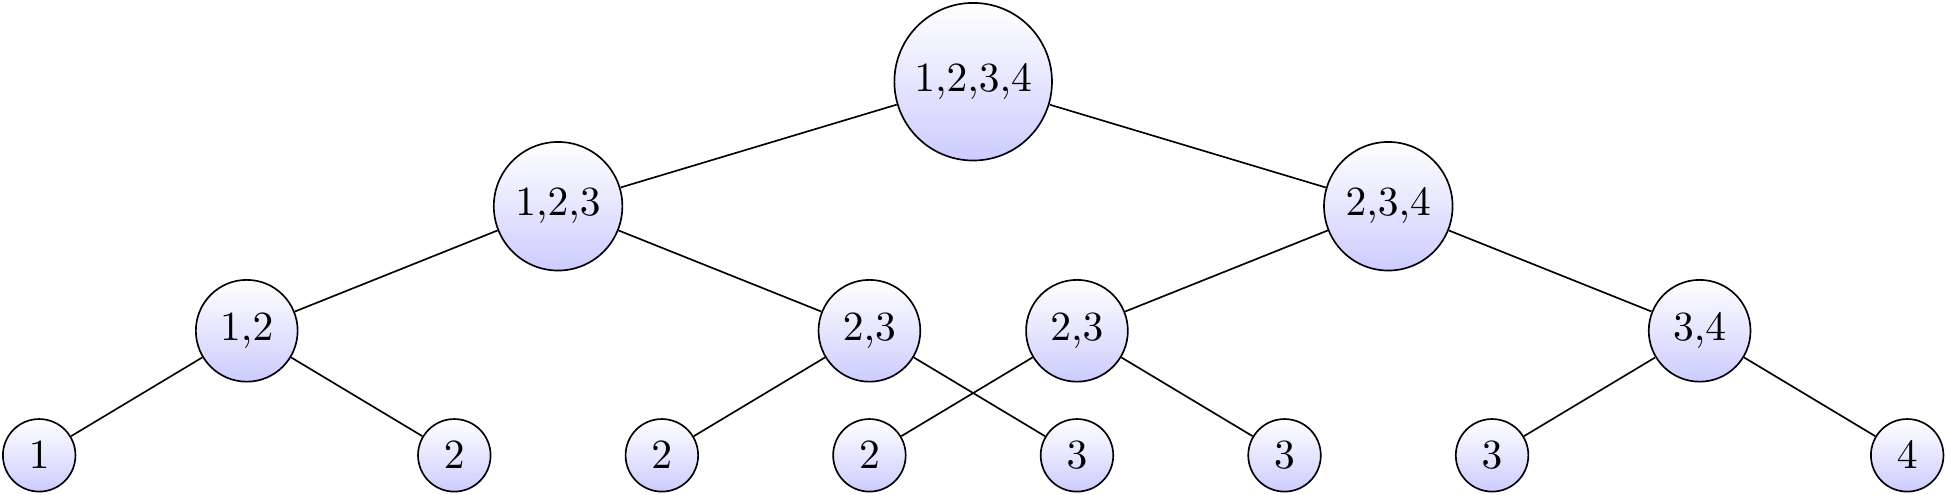
\includegraphics[width=0.9\linewidth]{tech-interview_files/figure-latex/unnamed-chunk-6-1} \caption{Some caption.}\label{fig:unnamed-chunk-6}
\end{figure}

\hypertarget{analysis-51}{%
\subsubsection{Analysis\}\textbackslash{}}\label{analysis-51}}

Naive recursive strategy results in overlapping subproblems. The time complexity is \(O(2^{log (m * n)})\)

\hypertarget{algorithm-51}{%
\subsubsection{Algorithm\}\textbackslash{}}\label{algorithm-51}}

recursive \ref{recursive}

\hypertarget{java-code---recursion-1}{%
\subsection{Java Code - Recursion\}}\label{java-code---recursion-1}}

\begin{Shaded}
\begin{Highlighting}[]
\KeywordTok{public} \DataTypeTok{int} \FunctionTok{uniquePaths}\NormalTok{(}\DataTypeTok{int}\NormalTok{ m, }\DataTypeTok{int}\NormalTok{ n) \{}
    \KeywordTok{return} \FunctionTok{rec}\NormalTok{(}\DecValTok{0}\NormalTok{, }\DecValTok{0}\NormalTok{, m, n);}
\NormalTok{\}}
\DataTypeTok{int} \FunctionTok{rec}\NormalTok{(}\DataTypeTok{int}\NormalTok{ i, }\DataTypeTok{int}\NormalTok{ j, }\DataTypeTok{int}\NormalTok{ rows, }\DataTypeTok{int}\NormalTok{ cols)\{}

    \KeywordTok{if}\NormalTok{(i == (rows - }\DecValTok{1}\NormalTok{) && j == (cols - }\DecValTok{1}\NormalTok{))\{}
        \CommentTok{//at bottom right}
        \KeywordTok{return} \DecValTok{1}\NormalTok{;}
\NormalTok{    \} }\KeywordTok{else} \KeywordTok{if}\NormalTok{(i < (rows - }\DecValTok{1}\NormalTok{) && j == (cols - }\DecValTok{1}\NormalTok{)) \{}
        \CommentTok{//at last column, moving downward}
        \KeywordTok{return} \FunctionTok{rec}\NormalTok{(i+}\DecValTok{1}\NormalTok{, j, rows, cols);}
\NormalTok{    \} }\KeywordTok{else} \KeywordTok{if}\NormalTok{(i == (rows - }\DecValTok{1}\NormalTok{) && j < (cols - }\DecValTok{1}\NormalTok{)) \{}
        \CommentTok{//at last row, moving rightward}
        \KeywordTok{return} \FunctionTok{rec}\NormalTok{(i, j+}\DecValTok{1}\NormalTok{, rows, cols);}
\NormalTok{    \} }\KeywordTok{else}\NormalTok{ \{}
        \CommentTok{//other place, get min of downward and rightward}
        \KeywordTok{return} \FunctionTok{rec}\NormalTok{(i+}\DecValTok{1}\NormalTok{, j, rows, cols) + }\FunctionTok{rec}\NormalTok{(i, j+}\DecValTok{1}\NormalTok{, rows, cols);}
\NormalTok{    \}}
\NormalTok{\}}
\end{Highlighting}
\end{Shaded}

\hypertarget{solution---dynamic-programming-1}{%
\subsection{Solution - Dynamic Programming\}}\label{solution---dynamic-programming-1}}

\hypertarget{walkthrough-47}{%
\subsubsection{Walkthrough\}\textbackslash{}}\label{walkthrough-47}}

Number of unique path to current cell equals to the sum of paths to the previous cells. For example, the matrix
representing \# of path to reach current cell. The weight at (1,2) equals to sum of (0,2) and (1,1)

\begin{Shaded}
\begin{Highlighting}[]
\DecValTok{1} \DecValTok{1} \DecValTok{1}
\DecValTok{1} \DecValTok{2} \DecValTok{3}
\end{Highlighting}
\end{Shaded}

\hypertarget{analysis-52}{%
\subsubsection{Analysis\}\textbackslash{}}\label{analysis-52}}

Time complexity is O(n * m) since each cell is visited once. A cache of size O(n * m ) is used to store visited cell
value.

\hypertarget{algorithm-52}{%
\subsubsection{Algorithm\}\textbackslash{}}\label{algorithm-52}}

dp \ref{dp}

\hypertarget{java-code---dynamic-programming-1}{%
\subsection{Java Code - Dynamic Programming\}}\label{java-code---dynamic-programming-1}}

\begin{Shaded}
\begin{Highlighting}[]
\KeywordTok{public} \DataTypeTok{int} \FunctionTok{uniquePaths}\NormalTok{(}\DataTypeTok{int}\NormalTok{ m, }\DataTypeTok{int}\NormalTok{ n) \{}
    \KeywordTok{if}\NormalTok{(m == }\DecValTok{0}\NormalTok{ || n == }\DecValTok{0}\NormalTok{) \{}
        \KeywordTok{return} \DecValTok{0}\NormalTok{;}
\NormalTok{    \}}
    \KeywordTok{if}\NormalTok{(m == }\DecValTok{1}\NormalTok{ || n == }\DecValTok{1}\NormalTok{) \{}
        \KeywordTok{return} \DecValTok{1}\NormalTok{;}
\NormalTok{    \}}

    \DataTypeTok{int}\NormalTok{[][] dp = }\KeywordTok{new} \DataTypeTok{int}\NormalTok{[m][n];}

    \CommentTok{//init first column}
    \KeywordTok{for}\NormalTok{(}\DataTypeTok{int}\NormalTok{ i = }\DecValTok{0}\NormalTok{; i < m; i++)\{}
\NormalTok{        dp[i][}\DecValTok{0}\NormalTok{] = }\DecValTok{1}\NormalTok{;}
\NormalTok{    \}}

    \CommentTok{//init first row}
    \KeywordTok{for}\NormalTok{(}\DataTypeTok{int}\NormalTok{ j = }\DecValTok{0}\NormalTok{; j < n; j++)\{}
\NormalTok{        dp[}\DecValTok{0}\NormalTok{][j] = }\DecValTok{1}\NormalTok{;}
\NormalTok{    \}}

    \CommentTok{//fill up the rest of table}
    \KeywordTok{for}\NormalTok{(}\DataTypeTok{int}\NormalTok{ i = }\DecValTok{1}\NormalTok{; i < m; i++)\{}
        \KeywordTok{for}\NormalTok{(}\DataTypeTok{int}\NormalTok{ j = }\DecValTok{1}\NormalTok{; j < n; j++)\{}
\NormalTok{            dp[i][j] = dp[i - }\DecValTok{1}\NormalTok{][j] + dp[i][j - }\DecValTok{1}\NormalTok{];}
\NormalTok{        \}}
\NormalTok{    \}}

    \KeywordTok{return}\NormalTok{ dp[m}\DecValTok{-1}\NormalTok{][n}\DecValTok{-1}\NormalTok{];}
\NormalTok{\}}
\end{Highlighting}
\end{Shaded}

\hypertarget{word-search-leetcode-79-medium}{%
\section{Word Search / LeetCode 79 / Medium\}}\label{word-search-leetcode-79-medium}}

\hypertarget{description-47}{%
\subsection{Description\}}\label{description-47}}

Given a 2D board and a word, find if the word exists in the grid.

The word can be constructed from letters of sequentially adjacent cell, where ``adjacent'' cells are those
horizontally or vertically neighboring. The same letter cell may not be used more than once.

\hypertarget{example-45}{%
\subsection{Example\}}\label{example-45}}

\begin{verbatim}
board =
[
['A','B','C','E'],
['S','F','C','S'],
['A','D','E','E']
]
\end{verbatim}

Given word = ``ABCCED'', return true.
Given word = ``SEE'', return true.
Given word = ``ABCB'', return false.

\hypertarget{solution---dfs}{%
\subsection{Solution - DFS\}}\label{solution---dfs}}

\hypertarget{walkthrough-48}{%
\subsubsection{Walkthrough\}\textbackslash{}}\label{walkthrough-48}}

Enumerate all possible starting position from the 2D array by using two nested loops. While traversing the character
in the taget string, perform a search recursively on neighboring cells {[}(i, j + 1), (i, j - 1), (i + 1, j), (i - 1, j){]}.
If there is a hit in any four neighboring cells, return true; otherwise, return false.

\hypertarget{analysis-53}{%
\subsubsection{Analysis\}\textbackslash{}}\label{analysis-53}}

The enumeration cost is exponential, as there are multiple overlapping subproblems. Thus, the time complexity is
\(O(2^{log(n)})\)

\hypertarget{algorithm-53}{%
\subsubsection{Algorithm\}\textbackslash{}}\label{algorithm-53}}

backtrack \ref{backtrack}, dfs \ref{dfs}

\hypertarget{java-code---dfs}{%
\subsection{Java Code - DFS\}}\label{java-code---dfs}}

\begin{Shaded}
\begin{Highlighting}[]
\KeywordTok{private} \DataTypeTok{static} \DataTypeTok{final} \DataTypeTok{char}\NormalTok{ VISITED_CHARACTER = }\CharTok{'*'}\NormalTok{;}

\KeywordTok{public} \DataTypeTok{boolean} \FunctionTok{exist}\NormalTok{(}\DataTypeTok{char}\NormalTok{[][] board, }\BuiltInTok{String}\NormalTok{ word) \{}
    \DataTypeTok{int}\NormalTok{ numOfRows = board.}\FunctionTok{length}\NormalTok{;}
    \DataTypeTok{int}\NormalTok{ numOfCols = board[}\DecValTok{0}\NormalTok{].}\FunctionTok{length}\NormalTok{;}

    \CommentTok{//Enumerate the all possible starting position from char[][]}
    \KeywordTok{for}\NormalTok{ (}\DataTypeTok{int}\NormalTok{ i = }\DecValTok{0}\NormalTok{; i < numOfRows; i++) \{}
        \KeywordTok{for}\NormalTok{ (}\DataTypeTok{int}\NormalTok{ j = }\DecValTok{0}\NormalTok{; j < numOfCols; j++) \{}
            \KeywordTok{if}\NormalTok{ (}\FunctionTok{backtrack}\NormalTok{(board, i, j, word, }\DecValTok{0}\NormalTok{)) \{}
                \KeywordTok{return} \KeywordTok{true}\NormalTok{;}
\NormalTok{            \}}
\NormalTok{        \}}
\NormalTok{    \}}
    \KeywordTok{return} \KeywordTok{false}\NormalTok{;}
\NormalTok{\}}

\KeywordTok{private} \DataTypeTok{boolean} \FunctionTok{backtrack}\NormalTok{(}\DataTypeTok{char}\NormalTok{[][] board, }\DataTypeTok{int}\NormalTok{ row, }\DataTypeTok{int}\NormalTok{ col, }\BuiltInTok{String}\NormalTok{ word, }\DataTypeTok{int}\NormalTok{ index) \{}
    \DataTypeTok{int}\NormalTok{ numOfRows = board.}\FunctionTok{length}\NormalTok{;}
    \DataTypeTok{int}\NormalTok{ numOfCols = board[}\DecValTok{0}\NormalTok{].}\FunctionTok{length}\NormalTok{;}

    \CommentTok{//every other character has matched}
    \KeywordTok{if}\NormalTok{ (index == word.}\FunctionTok{length}\NormalTok{()) \{}
        \KeywordTok{return} \KeywordTok{true}\NormalTok{;}
\NormalTok{    \}}

    \CommentTok{//exceed the boundary}
    \KeywordTok{if}\NormalTok{ (row < }\DecValTok{0}\NormalTok{ || row >= numOfRows || col < }\DecValTok{0}\NormalTok{ || col >= numOfCols) \{}
        \KeywordTok{return} \KeywordTok{false}\NormalTok{;}
\NormalTok{    \}}

    \CommentTok{//if current char is not equal}
    \KeywordTok{if}\NormalTok{ (board[row][col] != word.}\FunctionTok{charAt}\NormalTok{(index)) \{}
        \KeywordTok{return} \KeywordTok{false}\NormalTok{;}
\NormalTok{    \}}

    \CommentTok{// 'nullify' current position}
\NormalTok{    board[row][col] ^= VISITED_CHARACTER;}

    \CommentTok{//result of next move from four directions.}
    \DataTypeTok{boolean}\NormalTok{ result = }\FunctionTok{backtrack}\NormalTok{(board, row + }\DecValTok{1}\NormalTok{, col, word, index + }\DecValTok{1}\NormalTok{)}
\NormalTok{                || }\FunctionTok{backtrack}\NormalTok{(board, row - }\DecValTok{1}\NormalTok{, col, word, index + }\DecValTok{1}\NormalTok{)}
\NormalTok{                || }\FunctionTok{backtrack}\NormalTok{(board, row, col + }\DecValTok{1}\NormalTok{, word, index + }\DecValTok{1}\NormalTok{)}
\NormalTok{                || }\FunctionTok{backtrack}\NormalTok{(board, row, col - }\DecValTok{1}\NormalTok{, word, index + }\DecValTok{1}\NormalTok{);}

    \CommentTok{//nullify back}
\NormalTok{    board[row][col] ^= VISITED_CHARACTER;}

    \KeywordTok{return}\NormalTok{ result;}
\NormalTok{\}}
\end{Highlighting}
\end{Shaded}

\hypertarget{number-of-islands-leetcode-200-medium}{%
\section{Number of Islands / LeetCode 200 / Medium\}}\label{number-of-islands-leetcode-200-medium}}

\hypertarget{description-48}{%
\subsection{Description\}}\label{description-48}}

Given a 2d grid map of '1's (land) and '0's (water), count the number of islands. An island is surrounded by water
and is formed by connecting adjacent lands horizontally or vertically. You may assume all four edges of the grid are
all surrounded by water.

\hypertarget{example-46}{%
\subsection{Example\}}\label{example-46}}

\begin{verbatim}
11110
11010
11000
00000
\end{verbatim}

= 1

\begin{verbatim}
11000
11000
00100
00011
\end{verbatim}

= 3
\#\#\# Solution - DFS\}
\#\#\#\# Walkthrough\}\textbackslash{}
Traverse all cell and once we find a land tile, fill the adjacent land recursively. Count each land tile we have
encountered.

\hypertarget{analysis-54}{%
\subsubsection{Analysis\}\textbackslash{}}\label{analysis-54}}

Everyone cell in matrix is visited. Thus, is O(rows * cols)

\hypertarget{algorithm-54}{%
\subsubsection{Algorithm\}\textbackslash{}}\label{algorithm-54}}

dfs \ref{dfs}

\hypertarget{java-code---dfs-1}{%
\subsection{Java Code - DFS\}}\label{java-code---dfs-1}}

\begin{Shaded}
\begin{Highlighting}[]
\KeywordTok{public} \DataTypeTok{int} \FunctionTok{numIslands}\NormalTok{(}\DataTypeTok{char}\NormalTok{[][] grid) \{}
    \KeywordTok{if}\NormalTok{(grid==}\KeywordTok{null}\NormalTok{ || grid.}\FunctionTok{length}\NormalTok{==}\DecValTok{0}\NormalTok{||grid[}\DecValTok{0}\NormalTok{].}\FunctionTok{length}\NormalTok{==}\DecValTok{0}\NormalTok{)}
        \KeywordTok{return} \DecValTok{0}\NormalTok{;}

    \DataTypeTok{int}\NormalTok{ rows = grid.}\FunctionTok{length}\NormalTok{;}
    \DataTypeTok{int}\NormalTok{ cols = grid[}\DecValTok{0}\NormalTok{].}\FunctionTok{length}\NormalTok{;}

    \DataTypeTok{int}\NormalTok{ count = }\DecValTok{0}\NormalTok{;}
    \KeywordTok{for}\NormalTok{(}\DataTypeTok{int}\NormalTok{ i = }\DecValTok{0}\NormalTok{; i < rows; i++)\{}
        \KeywordTok{for}\NormalTok{(}\DataTypeTok{int}\NormalTok{ j = }\DecValTok{0}\NormalTok{; j < cols; j++)\{}
            \KeywordTok{if}\NormalTok{(grid[i][j] == }\CharTok{'1'}\NormalTok{)\{}
\NormalTok{                count++;}
                \FunctionTok{fill}\NormalTok{(grid, i, j);}
\NormalTok{            \}}
\NormalTok{        \}}
\NormalTok{    \}}


    \KeywordTok{return}\NormalTok{ count;}
\NormalTok{\}}

\KeywordTok{public} \DataTypeTok{void} \FunctionTok{fill}\NormalTok{(}\DataTypeTok{char}\NormalTok{[][] grid, }\DataTypeTok{int}\NormalTok{ i, }\DataTypeTok{int}\NormalTok{ j)\{}
    \DataTypeTok{int}\NormalTok{ rows = grid.}\FunctionTok{length}\NormalTok{;}
    \DataTypeTok{int}\NormalTok{ cols = grid[}\DecValTok{0}\NormalTok{].}\FunctionTok{length}\NormalTok{;}

    \KeywordTok{if}\NormalTok{(i < }\DecValTok{0}\NormalTok{ || i >= rows || j < }\DecValTok{0}\NormalTok{ || j >= cols || grid[i][j] != }\CharTok{'1'}\NormalTok{)}
        \KeywordTok{return}\NormalTok{;}

\NormalTok{    grid[i][j] = }\CharTok{'X'}\NormalTok{;}

    \CommentTok{// recursively fill the adjacent land}
    \FunctionTok{fill}\NormalTok{(grid, i - }\DecValTok{1}\NormalTok{, j);}
    \FunctionTok{fill}\NormalTok{(grid, i + }\DecValTok{1}\NormalTok{, j);}
    \FunctionTok{fill}\NormalTok{(grid, i, j - }\DecValTok{1}\NormalTok{);}
    \FunctionTok{fill}\NormalTok{(grid, i, j + }\DecValTok{1}\NormalTok{);}
\NormalTok{\}}
\end{Highlighting}
\end{Shaded}

\hypertarget{surrounded-regions-leetcode-130-medium}{%
\section{Surrounded Regions / LeetCode 130 / Medium\}}\label{surrounded-regions-leetcode-130-medium}}

Given a 2D board containing `X' and `O' (the letter O), capture all regions surrounded by `X'. A region is captured
by flipping all 'O's into 'X's in that surrounded region.

Surrounded regions shouldn't be on the border, which means that any `O' on the border of the board are not flipped to
`X'. Any `O' that is not on the border and it is not connected to an `O' on the border will be flipped to `X'. Two
cells are connected if they are adjacent cells connected horizontally or vertically.

\hypertarget{description-49}{%
\subsection{Description\}}\label{description-49}}

\hypertarget{example-47}{%
\subsection{Example\}}\label{example-47}}

\begin{verbatim}
X X X X
X O O X
X X O X
X O X X
\end{verbatim}

to

\begin{verbatim}
X X X X
X X X X
X X X X
X O X X
\end{verbatim}

\hypertarget{solution---dfs-1}{%
\subsection{Solution - DFS\}}\label{solution---dfs-1}}

\hypertarget{walkthrough-49}{%
\subsubsection{Walkthrough\}\textbackslash{}}\label{walkthrough-49}}

First preserve the border tile (or tile connected to a border ultimately) with `\#'.

\begin{verbatim}
X X X X
X O O X
X X O X
X # X X
\end{verbatim}

Traverse all cell by changing the inland tile (`O') to `X' and reset `\#' back to `O'.

\begin{verbatim}
X X X X
X X X X
X X X X
X O X X
\end{verbatim}

\hypertarget{analysis-55}{%
\subsubsection{Analysis\}\textbackslash{}}\label{analysis-55}}

All cell is visited a few times, thus, O(rows * cols).
\#\#\#\# Algorithm\}\textbackslash{}
dfs \ref{dfs}

\hypertarget{java-code---dfs-2}{%
\subsection{Java Code - DFS\}}\label{java-code---dfs-2}}

\begin{Shaded}
\begin{Highlighting}[]
\KeywordTok{public} \DataTypeTok{void} \FunctionTok{solve}\NormalTok{(}\DataTypeTok{char}\NormalTok{[][] board) \{}
    \KeywordTok{if}\NormalTok{(board == }\KeywordTok{null}\NormalTok{ || board.}\FunctionTok{length}\NormalTok{==}\DecValTok{0}\NormalTok{)}
        \KeywordTok{return}\NormalTok{;}

    \DataTypeTok{int}\NormalTok{ rows = board.}\FunctionTok{length}\NormalTok{;}
    \DataTypeTok{int}\NormalTok{ cols = board[}\DecValTok{0}\NormalTok{].}\FunctionTok{length}\NormalTok{;}

    \CommentTok{//preserve O's on left & right boarder}
    \KeywordTok{for}\NormalTok{(}\DataTypeTok{int}\NormalTok{ i = }\DecValTok{0}\NormalTok{;i < rows;i++)\{}
        \KeywordTok{if}\NormalTok{(board[i][}\DecValTok{0}\NormalTok{] == }\CharTok{'O'}\NormalTok{)\{}
            \FunctionTok{preserve}\NormalTok{(board, i, }\DecValTok{0}\NormalTok{);}
\NormalTok{        \}}

        \KeywordTok{if}\NormalTok{(board[i][cols - }\DecValTok{1}\NormalTok{] == }\CharTok{'O'}\NormalTok{)\{}
            \FunctionTok{preserve}\NormalTok{(board, i, n - }\DecValTok{1}\NormalTok{);}
\NormalTok{        \}}
\NormalTok{    \}}

    \CommentTok{//preserve O's on top & bottom boarder}
    \KeywordTok{for}\NormalTok{(}\DataTypeTok{int}\NormalTok{ j = }\DecValTok{0}\NormalTok{; j < cols; j++)\{}
        \KeywordTok{if}\NormalTok{(board[}\DecValTok{0}\NormalTok{][j] == }\CharTok{'O'}\NormalTok{)\{}
            \FunctionTok{preserve}\NormalTok{(board, }\DecValTok{0}\NormalTok{, j);}
\NormalTok{        \}}

        \KeywordTok{if}\NormalTok{(board[rows - }\DecValTok{1}\NormalTok{][j] == }\CharTok{'O'}\NormalTok{)\{}
            \FunctionTok{preserve}\NormalTok{(board, m - }\DecValTok{1}\NormalTok{, j);}
\NormalTok{        \}}
\NormalTok{    \}}

    \CommentTok{//process the board}
    \KeywordTok{for}\NormalTok{(}\DataTypeTok{int}\NormalTok{ i = }\DecValTok{0}\NormalTok{;i < rows;i++) \{}
        \KeywordTok{for}\NormalTok{(}\DataTypeTok{int}\NormalTok{ j = }\DecValTok{0}\NormalTok{; j < cols; j++) \{}
            \KeywordTok{if}\NormalTok{(board[i][j] == }\CharTok{'O'}\NormalTok{) \{}
\NormalTok{                board[i][j] = }\CharTok{'X'}\NormalTok{;}
\NormalTok{            \} }\KeywordTok{else} \KeywordTok{if}\NormalTok{(board[i][j] == }\CharTok{'#'}\NormalTok{) \{}
                \CommentTok{// change the preserved border tile back to 'O'}
\NormalTok{                board[i][j] = }\CharTok{'O'}\NormalTok{;}
\NormalTok{            \}}
\NormalTok{        \}}
\NormalTok{    \}}
\NormalTok{\}}

\KeywordTok{public} \DataTypeTok{void} \FunctionTok{preserve}\NormalTok{(}\DataTypeTok{char}\NormalTok{[][] board, }\DataTypeTok{int}\NormalTok{ i, }\DataTypeTok{int}\NormalTok{ j)\{}
    \DataTypeTok{int}\NormalTok{ rows = board.}\FunctionTok{length}\NormalTok{;}
    \DataTypeTok{int}\NormalTok{ cols = board[}\DecValTok{0}\NormalTok{].}\FunctionTok{length}\NormalTok{;}

    \KeywordTok{if}\NormalTok{(i < }\DecValTok{0}\NormalTok{ || i >= rows || j < }\DecValTok{0}\NormalTok{ || j >= cols || board[i][j] != }\CharTok{'O'}\NormalTok{)}
        \KeywordTok{return}\NormalTok{;}

\NormalTok{    board[i][j] = }\CharTok{'#'}\NormalTok{;}

    \CommentTok{// recursively fill the adjacent land}
    \FunctionTok{preserve}\NormalTok{(board, i - }\DecValTok{1}\NormalTok{, j);}
    \FunctionTok{preserve}\NormalTok{(board, i + }\DecValTok{1}\NormalTok{, j);}
    \FunctionTok{preserve}\NormalTok{(board, i, j - }\DecValTok{1}\NormalTok{);}
    \FunctionTok{preserve}\NormalTok{(board, i, j + }\DecValTok{1}\NormalTok{);}
\NormalTok{\}}
\end{Highlighting}
\end{Shaded}

\hypertarget{best-meeting-point-leetcode-296-hard}{%
\section{Best Meeting Point / LeetCode 296 / Hard\}}\label{best-meeting-point-leetcode-296-hard}}

\hypertarget{description-50}{%
\subsection{Description\}}\label{description-50}}

A group of two or more people wants to meet and minimize the total travel distance. You are given a 2D grid of values
0 or 1, where each 1 marks the home of someone in the group. The distance is calculated using Manhattan Distance, where
distance(p1, p2) = \(|p2.x - p1.x| + |p2.y - p1.y|\)

\hypertarget{example-48}{%
\subsection{Example\}}\label{example-48}}

For example, given three people living at (0,0), (0,4), and (2,2):

\begin{verbatim}
1 - 0 - [0] - 0 - 1
|   |     |     |   |
0 - 0 -   0 -  0 - 0
|   |     |     |   |
0 - 0 -   1 -  0 - 0
\end{verbatim}

The point (0,2) is an ideal meeting point, as the total travel distance of 2+2+2=6 is minimal. So return 6.
\#\#\# Solution\}
\#\#\#\# Walkthrough\}\textbackslash{}
The median points for row and col should be the optimal meeting point. We could compute the distance by substracting
the coordinate of people by the median X and Y.

\hypertarget{analysis-56}{%
\subsubsection{Analysis\}\textbackslash{}}\label{analysis-56}}

Each cell in matrix will be visited at least once. Thus, O(rows * cols).

\hypertarget{algorithm-55}{%
\subsubsection{Algorithm\}\textbackslash{}}\label{algorithm-55}}

\hypertarget{java-code-40}{%
\subsection{Java Code\}}\label{java-code-40}}

\begin{Shaded}
\begin{Highlighting}[]
\KeywordTok{public} \DataTypeTok{int} \FunctionTok{minTotalDistance}\NormalTok{(}\DataTypeTok{int}\NormalTok{[][] grid) \{}
    \DataTypeTok{int}\NormalTok{ rows = grid.}\FunctionTok{length}\NormalTok{;}
    \DataTypeTok{int}\NormalTok{ cols = grid[}\DecValTok{0}\NormalTok{].}\FunctionTok{length}\NormalTok{;}

    \BuiltInTok{List}\NormalTok{<}\BuiltInTok{Integer}\NormalTok{> cols = }\KeywordTok{new} \BuiltInTok{ArrayList}\NormalTok{<}\BuiltInTok{Integer}\NormalTok{>();}
    \BuiltInTok{List}\NormalTok{<}\BuiltInTok{Integer}\NormalTok{> rows = }\KeywordTok{new} \BuiltInTok{ArrayList}\NormalTok{<}\BuiltInTok{Integer}\NormalTok{>();}
    \KeywordTok{for}\NormalTok{(}\DataTypeTok{int}\NormalTok{ i = }\DecValTok{0}\NormalTok{; i < rows; i++)\{}
        \KeywordTok{for}\NormalTok{(}\DataTypeTok{int}\NormalTok{ j = }\DecValTok{0}\NormalTok{; cols < n; j++)\{}
            \KeywordTok{if}\NormalTok{(grid[i][j] == }\DecValTok{1}\NormalTok{)\{}
\NormalTok{                cols.}\FunctionTok{add}\NormalTok{(j);}
\NormalTok{                rows.}\FunctionTok{add}\NormalTok{(i);}
\NormalTok{            \}}
\NormalTok{        \}}
\NormalTok{    \}}

    \DataTypeTok{int}\NormalTok{ dist = }\DecValTok{0}\NormalTok{;}

    \DataTypeTok{int}\NormalTok{ medianRow = rows.}\FunctionTok{get}\NormalTok{(rows.}\FunctionTok{size}\NormalTok{() / }\DecValTok{2}\NormalTok{);}
    \KeywordTok{for}\NormalTok{(}\BuiltInTok{Integer}\NormalTok{ r: rows)\{}
\NormalTok{        dist += }\BuiltInTok{Math}\NormalTok{.}\FunctionTok{abs}\NormalTok{(r - medianRow);}
\NormalTok{    \}}

    \CommentTok{//sort col position so that we could get median col properly}
    \BuiltInTok{Collections}\NormalTok{.}\FunctionTok{sort}\NormalTok{(cols);}
    \DataTypeTok{int}\NormalTok{ medianCol = cols.}\FunctionTok{get}\NormalTok{(cols.}\FunctionTok{size}\NormalTok{() / }\DecValTok{2}\NormalTok{);}

    \KeywordTok{for}\NormalTok{(}\BuiltInTok{Integer}\NormalTok{ c: cols)\{}
\NormalTok{        dist += }\BuiltInTok{Math}\NormalTok{.}\FunctionTok{abs}\NormalTok{(c - medianCol);}
\NormalTok{    \}}

    \KeywordTok{return}\NormalTok{ dist;}
\NormalTok{\}}
\end{Highlighting}
\end{Shaded}

\hypertarget{tree}{%
\chapter{Tree}\label{tree}}

\hypertarget{breadth-first-traversal}{%
\subsection{Breadth First Traversal}\label{breadth-first-traversal}}

The algorithm starts at the tree root, and explores all of the neighbor nodes at the present depth prior to moving
on to the nodes at the next depth level.

\hypertarget{algorithm-56}{%
\subsubsection{Algorithm\textbackslash{}}\label{algorithm-56}}

bfs \ref{bfs}

\hypertarget{typical-implementation---java}{%
\subsubsection{Typical Implementation - Java}\label{typical-implementation---java}}

\begin{Shaded}
\begin{Highlighting}[]
\KeywordTok{public} \DataTypeTok{boolean} \FunctionTok{breadthFirstTraversal}\NormalTok{(}\BuiltInTok{TreeNode}\NormalTok{ root) \{}
    \BuiltInTok{Queue}\NormalTok{<}\BuiltInTok{TreeNode}\NormalTok{> queue = }\KeywordTok{new} \BuiltInTok{LinkedList}\NormalTok{();}

    \KeywordTok{while}\NormalTok{ (!queue.}\FunctionTok{isEmpty}\NormalTok{()) \{}
        \BuiltInTok{TreeNode}\NormalTok{ node = queue.}\FunctionTok{poll}\NormalTok{();}

        \KeywordTok{if}\NormalTok{ (node.}\FunctionTok{left}\NormalTok{ != }\KeywordTok{null}\NormalTok{) \{}
\NormalTok{            queue.}\FunctionTok{offer}\NormalTok{(node.}\FunctionTok{left}\NormalTok{);}
\NormalTok{        \}}

        \KeywordTok{if}\NormalTok{ (node.}\FunctionTok{right}\NormalTok{ != }\KeywordTok{null}\NormalTok{) \{}
\NormalTok{            queue.}\FunctionTok{offer}\NormalTok{(node.}\FunctionTok{right}\NormalTok{);}
\NormalTok{        \}}
\NormalTok{    \}}

    \KeywordTok{return} \KeywordTok{false}\NormalTok{;}
\NormalTok{\}}
\end{Highlighting}
\end{Shaded}

\hypertarget{complexity-analysis}{%
\subsubsection{Complexity Analysis}\label{complexity-analysis}}

\begin{itemize}
\tightlist
\item
  Time Complexity: Breadth-first search visits every vertex once and checks every edge in the graph once.
  Therefore, the runtime complexity is \(O(|V| + |E|)\). In simplicity, O(n) since \(|V| = n\)
\item
  Auxiliary Space: In Breadth First traversal, visited node in different level is stored in a queue one by one.
  Extra Space required is O(w) where w is maximum width of a level in binary tree.
\end{itemize}

\hypertarget{depth-first-traversal}{%
\subsection{Depth First Traversal}\label{depth-first-traversal}}

The algorithm starts at the root node and explores as far as possible along each branch.

\hypertarget{algorithm-57}{%
\subsubsection{Algorithm}\label{algorithm-57}}

dfs \ref{dfs}

\hypertarget{type-of-depth-first-traversal}{%
\subsubsection{Type of Depth First Traversal}\label{type-of-depth-first-traversal}}

\begin{itemize}
\item
  \hyperref[sec:depth_first_inorder]{Depth First InOrder Traversal}
\item
  \hyperref[sec:depth_first_preorder]{Depth First PreOrder Traversal}
\item
  \hyperref[sec:depth_first_postorder]{Depth First PostOrder Traversal}
\end{itemize}

\hypertarget{complexity-analysis-1}{%
\subsubsection{Complexity Analysis}\label{complexity-analysis-1}}

\begin{itemize}
\tightlist
\item
  Time Complexity: Depth-first search visits every vertex once and checks every edge in the graph once.
  Therefore, the runtime complexity is \(O(|V| + |E|)\). In simplicity, O(n) since \(|V| = n\)
\item
  Auxiliary Space: In Depth First Traversals, stack (or function call stack) stores all ancestors of a node. Extra Space required is O(h) where h is maximum height of binary tree.
\end{itemize}

\hypertarget{selection-strategy}{%
\subsection{Selection Strategy}\label{selection-strategy}}

\begin{itemize}
\tightlist
\item
  Extra Space can be one factor
\item
  Depth First Traversals are typically recursive and recursive code requires function call overheads.
\item
  The most important points is, BFS starts visiting nodes from root while DFS starts visiting nodes from leaves. So if our problem is to search something that is more likely to closer to root, we would prefer BFS. And if the target node is close to a leaf, we would prefer DFS
\item
  Maximum Width of a Binary Tree at depth (or height) h can be 2h where h starts from 0. So the maximum number of nodes can be at the last level. And worst case occurs when Binary Tree is a perfect Binary Tree with numbers of node
\item
  It is evident from above points that extra space required for Level order traversal is likely to be more when tree is more balanced and extra space for Depth First Traversal is likely to be more when tree is less balanced.
\end{itemize}

\hypertarget{binary-search-tree}{%
\subsection{Binary Search Tree}\label{binary-search-tree}}

\begin{figure}
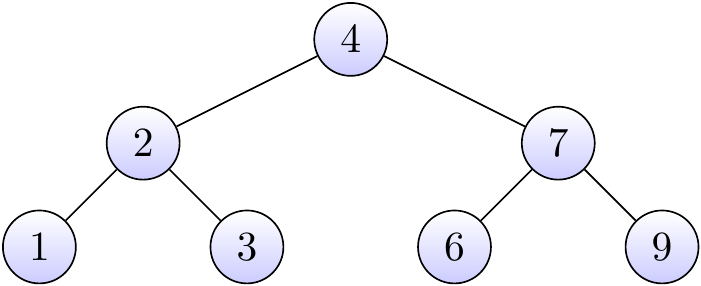
\includegraphics[width=0.9\linewidth]{tech-interview_files/figure-latex/unnamed-chunk-7-1} \caption{Some caption.}\label{fig:unnamed-chunk-7}
\end{figure}

A BST is a binary tree where nodes are ordered in the following way:

\begin{itemize}
\tightlist
\item
  each node contains one key (also known as data)
\item
  the keys in the left subtree are less then the key in its parent node
\item
  the keys in the right subtree are greater the key in its parent node
\item
  duplicate keys are not allowed.
\end{itemize}

\hypertarget{algorithm-58}{%
\subsubsection{Algorithm}\label{algorithm-58}}

bst \ref{bst}

\hypertarget{complexity-analysis-2}{%
\subsubsection{Complexity Analysis}\label{complexity-analysis-2}}

The particular kind of binary tree is optimized in a way that only a PARTIAL nodes along a path will be visited during
search, the general time complexity is reduced to O(h) where h = log(n).

Since a binary search tree with n nodes has a minimum of O(log(n)) levels, it takes at least O(log(n)) comparisons to
find a particular node. However, in the edge cases where tree is in a list form, the worst time complexity is O(n)

\hypertarget{balanced-binary-tree-leet-code-110-easy}{%
\section{Balanced Binary Tree / Leet Code 110 / Easy}\label{balanced-binary-tree-leet-code-110-easy}}

\hypertarget{description-51}{%
\subsection{Description}\label{description-51}}

Given a binary tree, determine if it is height-balanced. For this problem, a height-balanced binary tree is defined
as: a binary tree in which the depth of the two subtrees of every node never differ by more than 1.

\hypertarget{example-49}{%
\subsection{Example}\label{example-49}}

\begin{figure}
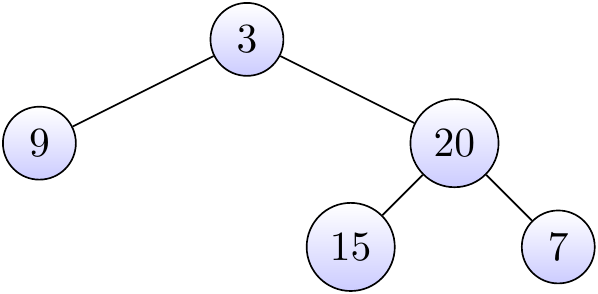
\includegraphics[width=0.9\linewidth]{tech-interview_files/figure-latex/unnamed-chunk-8-1} \caption{Some caption.}\label{fig:unnamed-chunk-8}
\end{figure}

Return true.

\begin{figure}
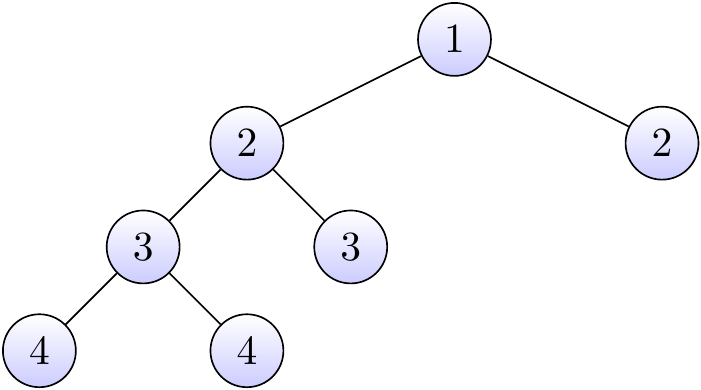
\includegraphics[width=0.9\linewidth]{tech-interview_files/figure-latex/unnamed-chunk-9-1} \caption{Some caption.}\label{fig:unnamed-chunk-9}
\end{figure}

Return false.

\hypertarget{solution-35}{%
\subsection{Solution}\label{solution-35}}

\hypertarget{walkthrough-50}{%
\subsubsection{Walkthrough\textbackslash{}}\label{walkthrough-50}}

Remember current height and recursively compute the height for the left and right subtree. In
addition, evaluate if the absolute value of height of two subtrees is greater than 1. If yes, return false; true,
otherwise.

\hypertarget{analysis-57}{%
\subsubsection{Analysis\textbackslash{}}\label{analysis-57}}

Time complexity is O(n) as every node is visited once.

\hypertarget{algorithm-59}{%
\subsubsection{Algorithm\textbackslash{}}\label{algorithm-59}}

dfs \ref{dfs}

\hypertarget{java-code-41}{%
\subsection{Java Code}\label{java-code-41}}

\begin{Shaded}
\begin{Highlighting}[]
\KeywordTok{public} \DataTypeTok{boolean} \FunctionTok{isBalanced}\NormalTok{(}\BuiltInTok{TreeNode}\NormalTok{ root) \{}
    \KeywordTok{if}\NormalTok{ (root == }\KeywordTok{null}\NormalTok{) \{}
        \KeywordTok{return} \KeywordTok{true}\NormalTok{;}
\NormalTok{    \}}

    \CommentTok{// left height | right height > 1}
    \KeywordTok{if}\NormalTok{ (}\FunctionTok{getHeight}\NormalTok{(root) == }\DecValTok{-1}\NormalTok{) \{}
        \KeywordTok{return} \KeywordTok{false}\NormalTok{;}
\NormalTok{    \}}

    \KeywordTok{return} \KeywordTok{true}\NormalTok{;}
\NormalTok{\}}

\KeywordTok{public} \DataTypeTok{int} \FunctionTok{getHeight}\NormalTok{(}\BuiltInTok{TreeNode}\NormalTok{ root) \{}
    \KeywordTok{if}\NormalTok{ (root == }\KeywordTok{null}\NormalTok{) \{}
        \KeywordTok{return} \DecValTok{0}\NormalTok{;}
\NormalTok{    \}}

    \DataTypeTok{int}\NormalTok{ lHeight = }\FunctionTok{getHeight}\NormalTok{(root.}\FunctionTok{left}\NormalTok{);}
    \DataTypeTok{int}\NormalTok{ rHeight = }\FunctionTok{getHeight}\NormalTok{(root.}\FunctionTok{right}\NormalTok{);}

    \KeywordTok{if}\NormalTok{ (lHeight == }\DecValTok{-1}\NormalTok{ || rHeight == }\DecValTok{-1}\NormalTok{) \{}
        \KeywordTok{return} \DecValTok{-1}\NormalTok{;}
\NormalTok{    \}}

    \KeywordTok{if}\NormalTok{ (}\BuiltInTok{Math}\NormalTok{.}\FunctionTok{abs}\NormalTok{(left - right) > }\DecValTok{1}\NormalTok{) \{}
        \KeywordTok{return} \DecValTok{-1}\NormalTok{;}
\NormalTok{    \}}

    \KeywordTok{return} \BuiltInTok{Math}\NormalTok{.}\FunctionTok{max}\NormalTok{(left, right) + }\DecValTok{1}\NormalTok{;}
\NormalTok{\}}
\end{Highlighting}
\end{Shaded}

\hypertarget{invert-binary-tree-leet-code-226-easy}{%
\section{Invert Binary Tree / Leet Code 226 Easy}\label{invert-binary-tree-leet-code-226-easy}}

\hypertarget{description-52}{%
\subsection{Description}\label{description-52}}

Invert a binary tree

\hypertarget{example-50}{%
\subsection{Example}\label{example-50}}

\begin{figure}
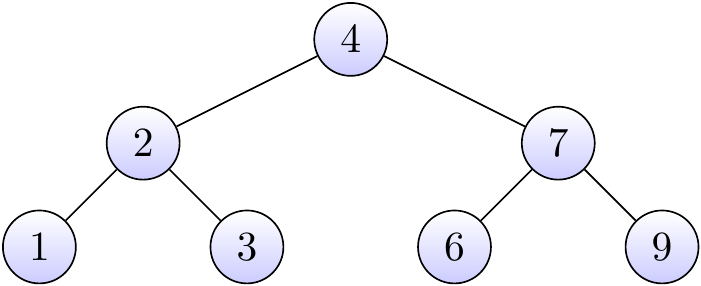
\includegraphics[width=0.9\linewidth]{tech-interview_files/figure-latex/unnamed-chunk-10-1} \caption{Some caption.}\label{fig:unnamed-chunk-10}
\end{figure}

inverts

\begin{figure}
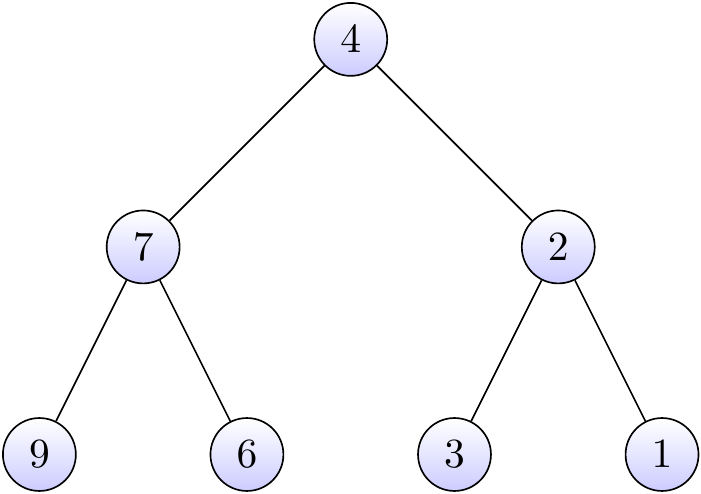
\includegraphics[width=0.9\linewidth]{tech-interview_files/figure-latex/unnamed-chunk-11-1} \caption{Some caption.}\label{fig:unnamed-chunk-11}
\end{figure}

\hypertarget{solution---dfs-2}{%
\subsection{Solution - DFS}\label{solution---dfs-2}}

\hypertarget{walkthrough-51}{%
\subsubsection{Walkthrough\textbackslash{}}\label{walkthrough-51}}

Swap the left and right subtree with recursive strategy.

\hypertarget{analysis-58}{%
\subsubsection{Analysis\textbackslash{}}\label{analysis-58}}

Time complexity is O(n) as every node is visited once.

\hypertarget{algorithm-60}{%
\subsubsection{Algorithm\textbackslash{}}\label{algorithm-60}}

dfs \ref{dfs}

\hypertarget{java-code---dfs-3}{%
\subsection{Java Code - DFS}\label{java-code---dfs-3}}

\begin{Shaded}
\begin{Highlighting}[]
\KeywordTok{public} \BuiltInTok{TreeNode} \FunctionTok{invertTree}\NormalTok{(}\BuiltInTok{TreeNode}\NormalTok{ root) \{}
    \KeywordTok{if}\NormalTok{ (root == }\KeywordTok{null}\NormalTok{) \{}
        \KeywordTok{return} \KeywordTok{null}\NormalTok{;}
\NormalTok{    \}}

    \CommentTok{//swap left and right subtrees}
    \BuiltInTok{TreeNode}\NormalTok{ origRight = root.}\FunctionTok{right}\NormalTok{;}
\NormalTok{    root.}\FunctionTok{right}\NormalTok{ = }\FunctionTok{invertTree}\NormalTok{(root.}\FunctionTok{left}\NormalTok{);}
\NormalTok{    root.}\FunctionTok{left}\NormalTok{ = }\FunctionTok{invertTree}\NormalTok{(origRight);}

    \KeywordTok{return}\NormalTok{ root;}
\NormalTok{\}}
\end{Highlighting}
\end{Shaded}

\hypertarget{solution---bfs}{%
\subsection{Solution - BFS}\label{solution---bfs}}

\hypertarget{walkthrough-52}{%
\subsubsection{Walkthrough\textbackslash{}}\label{walkthrough-52}}

Swap the left and right subtree with iterative (BFS) strategy

\hypertarget{analysis-59}{%
\subsubsection{Analysis\textbackslash{}}\label{analysis-59}}

Time complexity is O(n) as every node is visited once.

\hypertarget{algorithm-61}{%
\subsubsection{Algorithm\textbackslash{}}\label{algorithm-61}}

bfs \ref{bfs}

\hypertarget{java-code---bfs}{%
\subsection{Java Code - BFS}\label{java-code---bfs}}

\begin{Shaded}
\begin{Highlighting}[]
\KeywordTok{public} \BuiltInTok{TreeNode} \FunctionTok{invertTree}\NormalTok{(}\BuiltInTok{TreeNode}\NormalTok{ root) \{}
    \KeywordTok{if}\NormalTok{ (root == }\KeywordTok{null}\NormalTok{) \{}
        \KeywordTok{return} \KeywordTok{null}\NormalTok{;}
\NormalTok{    \}}

    \BuiltInTok{Queue}\NormalTok{<}\BuiltInTok{TreeNode}\NormalTok{> queue = }\KeywordTok{new} \BuiltInTok{LinkedList}\NormalTok{<}\BuiltInTok{TreeNode}\NormalTok{>();}
\NormalTok{    queue.}\FunctionTok{offer}\NormalTok{(root);}

    \KeywordTok{while}\NormalTok{(!queue.}\FunctionTok{isEmpty}\NormalTok{()) \{}
        \BuiltInTok{TreeNode}\NormalTok{ node = queue.}\FunctionTok{poll}\NormalTok{();}

        \CommentTok{//swap left and right subtrees}
        \BuiltInTok{TreeNode}\NormalTok{ origRight = node.}\FunctionTok{right}\NormalTok{;}
\NormalTok{        node.}\FunctionTok{right}\NormalTok{ = node.}\FunctionTok{left}\NormalTok{;}
\NormalTok{        node.}\FunctionTok{left}\NormalTok{ = origRight;}

        \KeywordTok{if}\NormalTok{ (node.}\FunctionTok{left}\NormalTok{ != }\KeywordTok{null}\NormalTok{) \{}
\NormalTok{            queue.}\FunctionTok{offer}\NormalTok{(node.}\FunctionTok{left}\NormalTok{);}
\NormalTok{        \}}
        \KeywordTok{if}\NormalTok{ (node.}\FunctionTok{right}\NormalTok{ != }\KeywordTok{null}\NormalTok{) \{}
\NormalTok{            queue.}\FunctionTok{offer}\NormalTok{(node.}\FunctionTok{right}\NormalTok{);}
\NormalTok{        \}}
\NormalTok{    \}}
    \KeywordTok{return}\NormalTok{ root;}
\NormalTok{\}}
\end{Highlighting}
\end{Shaded}

\hypertarget{symmetric-tree-leet-code-101-easy}{%
\section{Symmetric Tree / Leet Code 101 / Easy}\label{symmetric-tree-leet-code-101-easy}}

\hypertarget{description-53}{%
\subsection{Description}\label{description-53}}

Given a binary tree, check whether it is a mirror of itself (ie, symmetric around its center).

\hypertarget{example-51}{%
\subsection{Example}\label{example-51}}

\begin{figure}
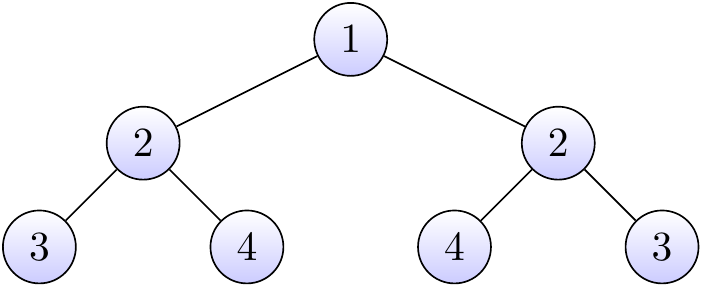
\includegraphics[width=0.9\linewidth]{tech-interview_files/figure-latex/unnamed-chunk-12-1} \caption{Some caption.}\label{fig:unnamed-chunk-12}
\end{figure}

is symmetric.

\begin{figure}
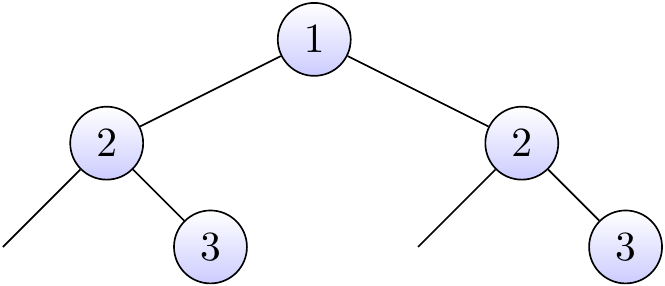
\includegraphics[width=0.9\linewidth]{tech-interview_files/figure-latex/unnamed-chunk-13-1} \caption{Some caption.}\label{fig:unnamed-chunk-13}
\end{figure}

is NOT symmetric.

\hypertarget{solution-36}{%
\subsection{Solution}\label{solution-36}}

\hypertarget{walkthrough-53}{%
\subsubsection{Walkthrough\textbackslash{}}\label{walkthrough-53}}

If they are symmetric, compare its value and recursively call its grand children node in symmetric manner:

\begin{itemize}
\tightlist
\item
  left.left vs right.right
\item
  left.right vs right.left
\end{itemize}

\hypertarget{analysis-60}{%
\subsubsection{Analysis\textbackslash{}}\label{analysis-60}}

Time complexity is O(n) as every node is visited once.

\hypertarget{algorithm-62}{%
\subsubsection{Algorithm\textbackslash{}}\label{algorithm-62}}

dfs \ref{dfs}

\hypertarget{java-code-42}{%
\subsection{Java Code}\label{java-code-42}}

\begin{Shaded}
\begin{Highlighting}[]
\KeywordTok{public} \DataTypeTok{boolean} \FunctionTok{isSymmetric}\NormalTok{(}\BuiltInTok{TreeNode}\NormalTok{ root) \{}
    \KeywordTok{if}\NormalTok{ (root == }\KeywordTok{null}\NormalTok{) \{}
        \KeywordTok{return} \KeywordTok{true}\NormalTok{;}
\NormalTok{    \}}
    \KeywordTok{return} \FunctionTok{isSymmetric}\NormalTok{(root.}\FunctionTok{left}\NormalTok{, root.}\FunctionTok{right}\NormalTok{);}
\NormalTok{\}}
\KeywordTok{private} \DataTypeTok{boolean} \FunctionTok{isSymmetric}\NormalTok{(}\BuiltInTok{TreeNode}\NormalTok{ left, }\BuiltInTok{TreeNode}\NormalTok{ right) \{}
    \KeywordTok{if}\NormalTok{ (left == }\KeywordTok{null}\NormalTok{ && right == }\KeywordTok{null}\NormalTok{) \{}
        \KeywordTok{return} \KeywordTok{true}\NormalTok{;}
\NormalTok{    \} }\KeywordTok{else} \KeywordTok{if}\NormalTok{ (left == }\KeywordTok{null}\NormalTok{ || right == }\KeywordTok{null}\NormalTok{) \{}
        \KeywordTok{return} \KeywordTok{false}\NormalTok{;}
\NormalTok{    \} }\KeywordTok{else}\NormalTok{ \{}
        \KeywordTok{return}\NormalTok{ left.}\FunctionTok{val}\NormalTok{ == right.}\FunctionTok{val}\NormalTok{ && }\FunctionTok{isSymmetric}\NormalTok{(left.}\FunctionTok{left}\NormalTok{, right.}\FunctionTok{right}\NormalTok{)}
\NormalTok{&& }\FunctionTok{isSymmetric}\NormalTok{(left.}\FunctionTok{right}\NormalTok{, right.}\FunctionTok{left}\NormalTok{);}
\NormalTok{    \}}

\NormalTok{\}}
\end{Highlighting}
\end{Shaded}

\hypertarget{binary-tree-level-order-traversal-leet-code-102-medium}{%
\section{Binary Tree Level Order Traversal / Leet Code 102 / Medium}\label{binary-tree-level-order-traversal-leet-code-102-medium}}

\hypertarget{description-54}{%
\subsection{Description}\label{description-54}}

Given a binary tree, return the level order traversal of its nodes' values. (ie, from left to right, level by
level).

\hypertarget{example-52}{%
\subsection{Example}\label{example-52}}

\begin{figure}
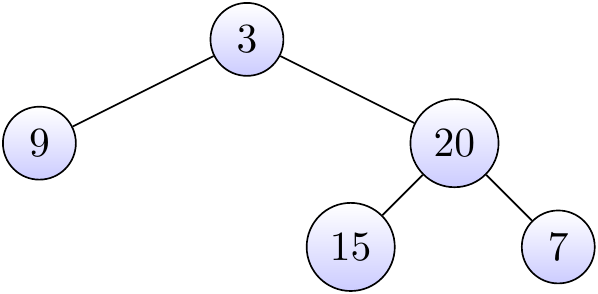
\includegraphics[width=0.9\linewidth]{tech-interview_files/figure-latex/unnamed-chunk-14-1} \caption{Some caption.}\label{fig:unnamed-chunk-14}
\end{figure}

return its level order traversal as:

\begin{verbatim}
[
    [3],
    [9,20],
    [15,7]
]
\end{verbatim}

\hypertarget{solution---bfs-with-two-loops}{%
\subsection{Solution - BFS with Two Loops}\label{solution---bfs-with-two-loops}}

\hypertarget{walkthrough-54}{%
\subsubsection{Walkthrough\textbackslash{}}\label{walkthrough-54}}

Create a queue and push node of the same level in a two dimensional array list while traversing the tree with
BFS algorithm.

\hypertarget{analysis-61}{%
\subsubsection{Analysis\textbackslash{}}\label{analysis-61}}

Breadth first traversal has time complexity of O(n), as every node is visited and thus the space
complexity is also O(n).

\hypertarget{algorithm-63}{%
\subsubsection{Algorithm\textbackslash{}}\label{algorithm-63}}

bfs \ref{bfs}

\hypertarget{java-code---bfs-with-two-loops}{%
\subsection{Java Code - BFS with Two Loops}\label{java-code---bfs-with-two-loops}}

\begin{Shaded}
\begin{Highlighting}[]
\KeywordTok{public} \BuiltInTok{List}\NormalTok{<}\BuiltInTok{List}\NormalTok{<}\BuiltInTok{Integer}\NormalTok{>> }\FunctionTok{levelOrder}\NormalTok{(}\BuiltInTok{TreeNode}\NormalTok{ root) \{}
    \BuiltInTok{Queue}\NormalTok{<}\BuiltInTok{TreeNode}\NormalTok{> queue = }\KeywordTok{new} \BuiltInTok{LinkedList}\NormalTok{<>();}
    \BuiltInTok{List}\NormalTok{<}\BuiltInTok{List}\NormalTok{<}\BuiltInTok{Integer}\NormalTok{>> levels = }\KeywordTok{new} \BuiltInTok{ArrayList}\NormalTok{<>();}

    \KeywordTok{if}\NormalTok{(root == }\KeywordTok{null}\NormalTok{) \{}
        \KeywordTok{return}\NormalTok{ levels;}
\NormalTok{    \}}

\NormalTok{    queue.}\FunctionTok{offer}\NormalTok{(root);}

    \KeywordTok{while}\NormalTok{(!queue.}\FunctionTok{isEmpty}\NormalTok{()) \{}
        \CommentTok{//number of element for this level}
        \DataTypeTok{int}\NormalTok{ currentLevelSize = queue.}\FunctionTok{size}\NormalTok{();}

        \BuiltInTok{List}\NormalTok{<}\BuiltInTok{Integer}\NormalTok{> level = }\KeywordTok{new} \BuiltInTok{ArrayList}\NormalTok{<>();}
        \KeywordTok{for}\NormalTok{(}\DataTypeTok{int}\NormalTok{ i = }\DecValTok{0}\NormalTok{; i < currentLevelSize; i++) \{}
            \BuiltInTok{TreeNode}\NormalTok{ node = queue.}\FunctionTok{poll}\NormalTok{();}
\NormalTok{            level.}\FunctionTok{add}\NormalTok{(node.}\FunctionTok{val}\NormalTok{);}

            \CommentTok{// push all elements for next level}
            \KeywordTok{if}\NormalTok{ (node.}\FunctionTok{left}\NormalTok{ != }\KeywordTok{null}\NormalTok{) \{}
\NormalTok{                queue.}\FunctionTok{offer}\NormalTok{(node.}\FunctionTok{left}\NormalTok{);}
\NormalTok{            \}}

            \KeywordTok{if}\NormalTok{ (node.}\FunctionTok{right}\NormalTok{ != }\KeywordTok{null}\NormalTok{) \{}
\NormalTok{                queue.}\FunctionTok{offer}\NormalTok{(node.}\FunctionTok{right}\NormalTok{);}
\NormalTok{            \}}
\NormalTok{        \}}

        \CommentTok{//add all elements for this level}
\NormalTok{        levels.}\FunctionTok{add}\NormalTok{(level);}
\NormalTok{    \}}

    \KeywordTok{return}\NormalTok{ levels;}
\NormalTok{\}}
\end{Highlighting}
\end{Shaded}

\hypertarget{solution---bfs-with-one-loops}{%
\subsection{Solution - BFS with One Loops}\label{solution---bfs-with-one-loops}}

\hypertarget{walkthrough-55}{%
\subsubsection{Walkthrough\textbackslash{}}\label{walkthrough-55}}

Create a queue and push node of the same level in a two dimensional array list while traversing the tree with
BFS algorithm.

\hypertarget{analysis-62}{%
\subsubsection{Analysis\textbackslash{}}\label{analysis-62}}

Breadth first traversal has time complexity of O(n), as every node is visited and thus the space
complexity is also O(n).

\hypertarget{algorithm-64}{%
\subsubsection{Algorithm\textbackslash{}}\label{algorithm-64}}

bfs \ref{bfs}

\hypertarget{java-code---bfs-with-one-loop}{%
\subsection{Java Code - BFS with One Loop}\label{java-code---bfs-with-one-loop}}

\begin{Shaded}
\begin{Highlighting}[]
\KeywordTok{public} \BuiltInTok{List}\NormalTok{<}\BuiltInTok{List}\NormalTok{<}\BuiltInTok{Integer}\NormalTok{>> }\FunctionTok{levelOrder}\NormalTok{(}\BuiltInTok{TreeNode}\NormalTok{ root) \{}
    \BuiltInTok{List}\NormalTok{<}\BuiltInTok{List}\NormalTok{<}\BuiltInTok{Integer}\NormalTok{>> levels = }\KeywordTok{new} \BuiltInTok{ArrayList}\NormalTok{<>();}
    \KeywordTok{if}\NormalTok{ (root == }\KeywordTok{null}\NormalTok{) \{}
        \KeywordTok{return}\NormalTok{ levels;}
\NormalTok{    \}}
    \BuiltInTok{Queue}\NormalTok{<}\BuiltInTok{TreeNode}\NormalTok{> currentLevelQueue = }\KeywordTok{new} \BuiltInTok{LinkedList}\NormalTok{<}\BuiltInTok{TreeNode}\NormalTok{>();}
    \BuiltInTok{Queue}\NormalTok{<}\BuiltInTok{TreeNode}\NormalTok{> nextLevelQueue = }\KeywordTok{new} \BuiltInTok{LinkedList}\NormalTok{<}\BuiltInTok{TreeNode}\NormalTok{>();}

\NormalTok{    currentLevelQueue.}\FunctionTok{offer}\NormalTok{(root);}
    \CommentTok{//init level to null}
    \BuiltInTok{List}\NormalTok{<}\BuiltInTok{Integer}\NormalTok{> level = }\KeywordTok{null}\NormalTok{;}

    \KeywordTok{while}\NormalTok{(!currentLevelQueue.}\FunctionTok{isEmpty}\NormalTok{()) \{}
        \BuiltInTok{TreeNode}\NormalTok{ node = currentLevelQueue.}\FunctionTok{poll}\NormalTok{();}

        \CommentTok{//starting a new level}
        \KeywordTok{if}\NormalTok{ (level == }\KeywordTok{null}\NormalTok{) \{}
\NormalTok{            level = }\KeywordTok{new} \BuiltInTok{LinkedList}\NormalTok{<}\BuiltInTok{Integer}\NormalTok{>();}
\NormalTok{            levels.}\FunctionTok{add}\NormalTok{(level);}
\NormalTok{        \}}
\NormalTok{        level.}\FunctionTok{add}\NormalTok{(node.}\FunctionTok{val}\NormalTok{);}

        \CommentTok{//push children to next level queue}
        \KeywordTok{if}\NormalTok{ (node.}\FunctionTok{left}\NormalTok{ != }\KeywordTok{null}\NormalTok{) \{}
\NormalTok{            nextLevelQueue.}\FunctionTok{offer}\NormalTok{(node.}\FunctionTok{left}\NormalTok{);}
\NormalTok{        \}}
        \KeywordTok{if}\NormalTok{ (node.}\FunctionTok{right}\NormalTok{ != }\KeywordTok{null}\NormalTok{) \{}
\NormalTok{            nextLevelQueue.}\FunctionTok{offer}\NormalTok{(node.}\FunctionTok{right}\NormalTok{);}
\NormalTok{        \}}

        \CommentTok{//swap queue and next, where next collects all nodes for next level}
        \KeywordTok{if}\NormalTok{ (currentLevelQueue.}\FunctionTok{isEmpty}\NormalTok{()) \{}
            \BuiltInTok{Queue}\NormalTok{<}\BuiltInTok{TreeNode}\NormalTok{> temp = currentLevelQueue;}
\NormalTok{            currentLevelQueue = nextLevelQueue;}
\NormalTok{            nextLevelQueue = temp;}
            \CommentTok{//init level to null}
\NormalTok{            level = }\KeywordTok{null}\NormalTok{;}
\NormalTok{        \}}
\NormalTok{    \}}
    \KeywordTok{return}\NormalTok{ levels;}
\NormalTok{\}}
\end{Highlighting}
\end{Shaded}

\hypertarget{solution---dfs-3}{%
\subsection{Solution - DFS}\label{solution---dfs-3}}

\hypertarget{walkthrough-56}{%
\subsubsection{Walkthrough\textbackslash{}}\label{walkthrough-56}}

We could traverse the tree recursively with \textbf{PreOrder} strategy, and additionally pass current level
into recursive method.

\hypertarget{analysis-63}{%
\subsubsection{Analysis\textbackslash{}}\label{analysis-63}}

DFS has time complexity of O(n) as every node is visited and thus Auxiliary Space is also O(n).

\hypertarget{algorithm-65}{%
\subsubsection{Algorithm\textbackslash{}}\label{algorithm-65}}

dfs \ref{dfs}

\hypertarget{java-code---dfs-4}{%
\subsection{Java Code - DFS}\label{java-code---dfs-4}}

\begin{Shaded}
\begin{Highlighting}[]
\KeywordTok{public} \BuiltInTok{List}\NormalTok{<}\BuiltInTok{List}\NormalTok{<}\BuiltInTok{Integer}\NormalTok{>> }\FunctionTok{levelOrder}\NormalTok{(}\BuiltInTok{TreeNode}\NormalTok{ root) \{}
    \BuiltInTok{List}\NormalTok{<}\BuiltInTok{List}\NormalTok{<}\BuiltInTok{Integer}\NormalTok{>> ans = }\KeywordTok{new} \BuiltInTok{ArrayList}\NormalTok{<>();}
    \FunctionTok{traverse}\NormalTok{(root, }\DecValTok{0}\NormalTok{, ans);}

    \KeywordTok{return}\NormalTok{ ans;}
\NormalTok{\}}

\KeywordTok{private} \DataTypeTok{void} \FunctionTok{traverse}\NormalTok{(}\BuiltInTok{TreeNode}\NormalTok{ root, }\DataTypeTok{int}\NormalTok{ level, }\BuiltInTok{List}\NormalTok{<}\BuiltInTok{List}\NormalTok{<}\BuiltInTok{Integer}\NormalTok{>> ans) \{}
    \KeywordTok{if}\NormalTok{(root == }\KeywordTok{null}\NormalTok{)\{}
        \KeywordTok{return}\NormalTok{;}
\NormalTok{    \}}

    \KeywordTok{if}\NormalTok{(ans.}\FunctionTok{size}\NormalTok{()<=level)\{}
\NormalTok{        ans.}\FunctionTok{add}\NormalTok{(}\KeywordTok{new} \BuiltInTok{ArrayList}\NormalTok{<>());}
\NormalTok{    \}}

\NormalTok{    ans.}\FunctionTok{get}\NormalTok{(level).}\FunctionTok{add}\NormalTok{(root.}\FunctionTok{val}\NormalTok{);}

    \FunctionTok{traverse}\NormalTok{(root.}\FunctionTok{left}\NormalTok{, level + }\DecValTok{1}\NormalTok{, ans);}
    \FunctionTok{traverse}\NormalTok{(root.}\FunctionTok{right}\NormalTok{, level + }\DecValTok{1}\NormalTok{, ans);}
\NormalTok{\}}
\end{Highlighting}
\end{Shaded}

\hypertarget{binary-tree-level-order-traversal-ii-leet-code-107-medium}{%
\section{Binary Tree Level Order Traversal II / Leet Code 107 / Medium}\label{binary-tree-level-order-traversal-ii-leet-code-107-medium}}

\hypertarget{description-55}{%
\subsection{Description}\label{description-55}}

Given a binary tree, return the bottom-up level order traversal of its nodes' values. (ie, from left to right, level by level from leaf
to root).

\hypertarget{example-53}{%
\subsection{Example}\label{example-53}}

\begin{figure}
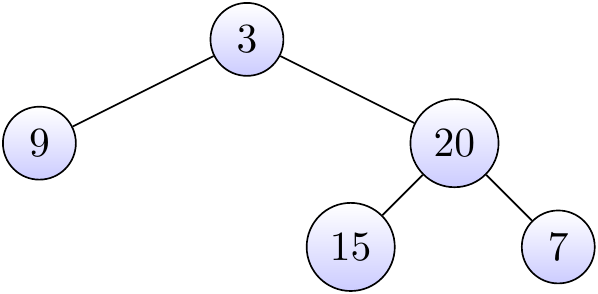
\includegraphics[width=0.9\linewidth]{tech-interview_files/figure-latex/unnamed-chunk-15-1} \caption{Some caption.}\label{fig:unnamed-chunk-15}
\end{figure}

return its level order traversal as:

\begin{verbatim}
[
    [15,7],
    [9,20],
    [3]
]
\end{verbatim}

\hypertarget{solution-37}{%
\subsection{Solution}\label{solution-37}}

\hypertarget{walkthrough-57}{%
\subsubsection{Walkthrough\textbackslash{}}\label{walkthrough-57}}

Create a queue and push node of the same level in a two dimensional array list while traversing the tree with
BFS algorithm. In addition, we only insert nodes at the first position at current level list.

\hypertarget{analysis-64}{%
\subsubsection{Analysis\textbackslash{}}\label{analysis-64}}

Time complexity is O(n) as every node is visited once.

\hypertarget{algorithm-66}{%
\subsubsection{Algorithm\textbackslash{}}\label{algorithm-66}}

bfs \ref{bfs}

\hypertarget{java-code---two-loops}{%
\subsection{Java Code - Two Loops}\label{java-code---two-loops}}

\begin{Shaded}
\begin{Highlighting}[]
\KeywordTok{public} \BuiltInTok{List}\NormalTok{<}\BuiltInTok{List}\NormalTok{<}\BuiltInTok{Integer}\NormalTok{>> }\FunctionTok{levelOrderBottom}\NormalTok{(}\BuiltInTok{TreeNode}\NormalTok{ root) \{}
    \BuiltInTok{Queue}\NormalTok{<}\BuiltInTok{TreeNode}\NormalTok{> queue = }\KeywordTok{new} \BuiltInTok{LinkedList}\NormalTok{<>();}
    \BuiltInTok{List}\NormalTok{<}\BuiltInTok{List}\NormalTok{<}\BuiltInTok{Integer}\NormalTok{>> levels = }\KeywordTok{new} \BuiltInTok{ArrayList}\NormalTok{<>();}

    \KeywordTok{if}\NormalTok{(root == }\KeywordTok{null}\NormalTok{) \{}
        \KeywordTok{return}\NormalTok{ levels;}
\NormalTok{    \}}

\NormalTok{    queue.}\FunctionTok{offer}\NormalTok{(root);}

    \KeywordTok{while}\NormalTok{(!queue.}\FunctionTok{isEmpty}\NormalTok{()) \{}
        \CommentTok{//number of element for this level}
        \DataTypeTok{int}\NormalTok{ currentLevelSize = queue.}\FunctionTok{size}\NormalTok{();}

        \BuiltInTok{List}\NormalTok{<}\BuiltInTok{Integer}\NormalTok{> level = }\KeywordTok{new} \BuiltInTok{ArrayList}\NormalTok{<>();}
        \KeywordTok{for}\NormalTok{(}\DataTypeTok{int}\NormalTok{ i = }\DecValTok{0}\NormalTok{; i < currentLevelSize; i++) \{}
            \BuiltInTok{TreeNode}\NormalTok{ node = queue.}\FunctionTok{poll}\NormalTok{();}
\NormalTok{            level.}\FunctionTok{add}\NormalTok{(node.}\FunctionTok{val}\NormalTok{);}

            \CommentTok{// push all elements for next level}
            \KeywordTok{if}\NormalTok{ (node.}\FunctionTok{left}\NormalTok{ != }\KeywordTok{null}\NormalTok{) \{}
\NormalTok{                queue.}\FunctionTok{offer}\NormalTok{(node.}\FunctionTok{left}\NormalTok{);}
\NormalTok{            \}}

            \KeywordTok{if}\NormalTok{ (node.}\FunctionTok{right}\NormalTok{ != }\KeywordTok{null}\NormalTok{) \{}
\NormalTok{                queue.}\FunctionTok{offer}\NormalTok{(node.}\FunctionTok{right}\NormalTok{);}
\NormalTok{            \}}
\NormalTok{        \}}

        \CommentTok{// insert the head of the list}
\NormalTok{        levels.}\FunctionTok{add}\NormalTok{(}\DecValTok{0}\NormalTok{, level);}
\NormalTok{    \}}

    \KeywordTok{return}\NormalTok{ levels;}
\NormalTok{\}}
\end{Highlighting}
\end{Shaded}

\hypertarget{walkthrough-58}{%
\subsubsection{Walkthrough\textbackslash{}}\label{walkthrough-58}}

Create a queue and push node of the same level in a two dimensional array list while traversing the tree with
BFS algorithm. In addition, we only insert nodes at the first position at current level list.

\hypertarget{analysis-65}{%
\subsubsection{Analysis\textbackslash{}}\label{analysis-65}}

Time complexity is O(n) as every node is visited once.

\hypertarget{algorithm-67}{%
\subsubsection{Algorithm\textbackslash{}}\label{algorithm-67}}

bfs \ref{bfs}

\hypertarget{java-code---one-loop}{%
\subsection{Java Code - One Loop}\label{java-code---one-loop}}

\begin{Shaded}
\begin{Highlighting}[]
\KeywordTok{public} \BuiltInTok{List}\NormalTok{<}\BuiltInTok{List}\NormalTok{<}\BuiltInTok{Integer}\NormalTok{>> }\FunctionTok{levelOrderBottom}\NormalTok{(}\BuiltInTok{TreeNode}\NormalTok{ root) \{}
    \BuiltInTok{List}\NormalTok{<}\BuiltInTok{List}\NormalTok{<}\BuiltInTok{Integer}\NormalTok{>> levels = }\KeywordTok{new} \BuiltInTok{ArrayList}\NormalTok{<>();}
    \KeywordTok{if}\NormalTok{ (root == }\KeywordTok{null}\NormalTok{) \{}
        \KeywordTok{return}\NormalTok{ levels;}
\NormalTok{    \}}

    \BuiltInTok{Queue}\NormalTok{<}\BuiltInTok{TreeNode}\NormalTok{> currentLevelQueue = }\KeywordTok{new} \BuiltInTok{LinkedList}\NormalTok{<}\BuiltInTok{TreeNode}\NormalTok{>();}
    \BuiltInTok{Queue}\NormalTok{<}\BuiltInTok{TreeNode}\NormalTok{> nextLevelQueue = }\KeywordTok{new} \BuiltInTok{LinkedList}\NormalTok{<}\BuiltInTok{TreeNode}\NormalTok{>();}

\NormalTok{    currentLevelQueue.}\FunctionTok{offer}\NormalTok{(root);}
    \CommentTok{//init level to null}
    \BuiltInTok{List}\NormalTok{<}\BuiltInTok{Integer}\NormalTok{> level = }\KeywordTok{null}\NormalTok{;}

    \KeywordTok{while}\NormalTok{ (!currentLevelQueue.}\FunctionTok{isEmpty}\NormalTok{()) \{}
        \BuiltInTok{TreeNode}\NormalTok{ node = currentLevelQueue.}\FunctionTok{poll}\NormalTok{();}

        \CommentTok{//starting a new level}
        \KeywordTok{if}\NormalTok{ (level == }\KeywordTok{null}\NormalTok{) \{}
\NormalTok{            level = }\KeywordTok{new} \BuiltInTok{LinkedList}\NormalTok{<}\BuiltInTok{Integer}\NormalTok{>();}
            \CommentTok{// insert to head}
\NormalTok{            levels.}\FunctionTok{add}\NormalTok{(}\DecValTok{0}\NormalTok{, level);}
\NormalTok{        \}}
\NormalTok{        level.}\FunctionTok{add}\NormalTok{(node.}\FunctionTok{val}\NormalTok{);}

        \CommentTok{//push children to next level queue}
        \KeywordTok{if}\NormalTok{ (node.}\FunctionTok{left}\NormalTok{ != }\KeywordTok{null}\NormalTok{) \{}
\NormalTok{            nextLevelQueue.}\FunctionTok{offer}\NormalTok{(node.}\FunctionTok{left}\NormalTok{);}
\NormalTok{        \}}
        \KeywordTok{if}\NormalTok{ (node.}\FunctionTok{right}\NormalTok{ != }\KeywordTok{null}\NormalTok{) \{}
\NormalTok{            nextLevelQueue.}\FunctionTok{offer}\NormalTok{(node.}\FunctionTok{right}\NormalTok{);}
\NormalTok{        \}}

        \CommentTok{//swap queue and next, where next collects all nodes for next level}
        \KeywordTok{if}\NormalTok{ (currentLevelQueue.}\FunctionTok{isEmpty}\NormalTok{()) \{}
            \BuiltInTok{Queue}\NormalTok{<}\BuiltInTok{TreeNode}\NormalTok{> temp = currentLevelQueue;}
\NormalTok{            currentLevelQueue = nextLevelQueue;}
\NormalTok{            nextLevelQueue = temp;}
            \CommentTok{//init level to null}
\NormalTok{            level = }\KeywordTok{null}\NormalTok{;}
\NormalTok{        \}}
\NormalTok{    \}}
    \KeywordTok{return}\NormalTok{ levels;}
\NormalTok{\}}
\end{Highlighting}
\end{Shaded}

\hypertarget{binary-tree-zigzag-level-order-traversal-leet-code-103-medium}{%
\section{Binary Tree Zigzag Level Order Traversal / Leet Code 103 / Medium}\label{binary-tree-zigzag-level-order-traversal-leet-code-103-medium}}

\hypertarget{description-56}{%
\subsection{Description}\label{description-56}}

Given a binary tree, return the zigzag level order traversal of its nodes' values. (ie, from left to right, then
right to left for the next level and alternate between).

\hypertarget{example-54}{%
\subsection{Example}\label{example-54}}

\begin{figure}
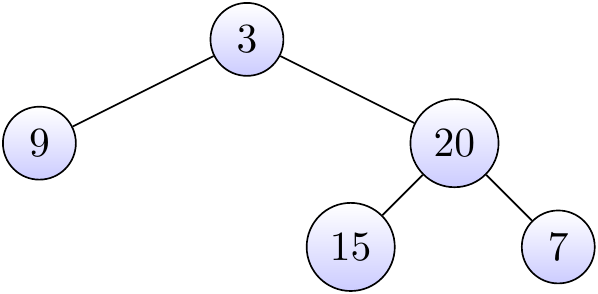
\includegraphics[width=0.9\linewidth]{tech-interview_files/figure-latex/unnamed-chunk-16-1} \caption{Some caption.}\label{fig:unnamed-chunk-16}
\end{figure}

return its level order traversal as:

\begin{verbatim}
[
    [3],
    [20,9],
    [15,7]
]
\end{verbatim}

\hypertarget{solution-38}{%
\subsection{Solution}\label{solution-38}}

\hypertarget{walkthrough-59}{%
\subsubsection{Walkthrough\textbackslash{}}\label{walkthrough-59}}

Create a queue and push node of the same level in a two dimensional array list while traversing the tree with
BFS algorithm. While pushing the value to the level, remember the current level and evaluate the zig-zag pattern.
That is, insert nodes for certain level at the first position at current level list.

\hypertarget{analysis-66}{%
\subsubsection{Analysis\textbackslash{}}\label{analysis-66}}

Time complexity is O(n) as every node is visited once.

\hypertarget{algorithm-68}{%
\subsubsection{Algorithm\textbackslash{}}\label{algorithm-68}}

bfs \ref{bfs}

\hypertarget{java-code---two-loops-1}{%
\subsection{Java Code - Two Loops}\label{java-code---two-loops-1}}

\begin{Shaded}
\begin{Highlighting}[]
\KeywordTok{public} \BuiltInTok{List}\NormalTok{<}\BuiltInTok{List}\NormalTok{<}\BuiltInTok{Integer}\NormalTok{>> }\FunctionTok{zigzagLevelOrder}\NormalTok{(}\BuiltInTok{TreeNode}\NormalTok{ root) \{}
    \BuiltInTok{Queue}\NormalTok{<}\BuiltInTok{TreeNode}\NormalTok{> queue = }\KeywordTok{new} \BuiltInTok{LinkedList}\NormalTok{<>();}
    \BuiltInTok{List}\NormalTok{<}\BuiltInTok{List}\NormalTok{<}\BuiltInTok{Integer}\NormalTok{>> levels = }\KeywordTok{new} \BuiltInTok{ArrayList}\NormalTok{<>();}

    \KeywordTok{if}\NormalTok{(root == }\KeywordTok{null}\NormalTok{) \{}
        \KeywordTok{return}\NormalTok{ levels;}
\NormalTok{    \}}

\NormalTok{    queue.}\FunctionTok{offer}\NormalTok{(root);}
    \DataTypeTok{int}\NormalTok{ levelNum = }\DecValTok{1}\NormalTok{;}

    \KeywordTok{while}\NormalTok{(!queue.}\FunctionTok{isEmpty}\NormalTok{()) \{}
        \CommentTok{//number of element for this level}
        \DataTypeTok{int}\NormalTok{ currentLevelSize = queue.}\FunctionTok{size}\NormalTok{();}
        \BuiltInTok{List}\NormalTok{<}\BuiltInTok{Integer}\NormalTok{> level = }\KeywordTok{new} \BuiltInTok{ArrayList}\NormalTok{<>();}

        \KeywordTok{for}\NormalTok{(}\DataTypeTok{int}\NormalTok{ i = }\DecValTok{0}\NormalTok{; i < currentLevelSize; i++) \{}
            \BuiltInTok{TreeNode}\NormalTok{ node = queue.}\FunctionTok{poll}\NormalTok{();}

            \KeywordTok{if}\NormalTok{(levelNum % }\DecValTok{2}\NormalTok{ != }\DecValTok{0}\NormalTok{) \{}
\NormalTok{                level.}\FunctionTok{add}\NormalTok{(node.}\FunctionTok{val}\NormalTok{);}
\NormalTok{            \} }\KeywordTok{else}\NormalTok{ \{}
\NormalTok{                level.}\FunctionTok{add}\NormalTok{(}\DecValTok{0}\NormalTok{, node.}\FunctionTok{val}\NormalTok{);}
\NormalTok{            \}}

            \CommentTok{// push all elements for next level}
            \KeywordTok{if}\NormalTok{ (node.}\FunctionTok{left}\NormalTok{ != }\KeywordTok{null}\NormalTok{) \{}
\NormalTok{                queue.}\FunctionTok{offer}\NormalTok{(node.}\FunctionTok{left}\NormalTok{);}
\NormalTok{            \}}

            \KeywordTok{if}\NormalTok{ (node.}\FunctionTok{right}\NormalTok{ != }\KeywordTok{null}\NormalTok{) \{}
\NormalTok{                queue.}\FunctionTok{offer}\NormalTok{(node.}\FunctionTok{right}\NormalTok{);}
\NormalTok{            \}}
\NormalTok{        \}}
\NormalTok{        levelNum++;}

\NormalTok{        levels.}\FunctionTok{add}\NormalTok{(level);}
\NormalTok{    \}}

    \KeywordTok{return}\NormalTok{ levels;}
\NormalTok{\}}
\end{Highlighting}
\end{Shaded}

\hypertarget{walkthrough-60}{%
\subsubsection{Walkthrough\textbackslash{}}\label{walkthrough-60}}

Create a queue and push node of the same level in a two dimensional array list while traversing the tree with
BFS algorithm. While pushing the value to the level, remember the current level and evaluate the zig-zag pattern.

\hypertarget{analysis-67}{%
\subsubsection{Analysis\textbackslash{}}\label{analysis-67}}

Time complexity is O(n) as every node is visited once.

\hypertarget{algorithm-69}{%
\subsubsection{Algorithm\textbackslash{}}\label{algorithm-69}}

bfs \ref{bfs}

\hypertarget{java-code---one-loop-1}{%
\subsection{Java Code - One Loop}\label{java-code---one-loop-1}}

\begin{Shaded}
\begin{Highlighting}[]
\KeywordTok{public} \BuiltInTok{List}\NormalTok{<}\BuiltInTok{List}\NormalTok{<}\BuiltInTok{Integer}\NormalTok{>> }\FunctionTok{zigzagLevelOrder}\NormalTok{(}\BuiltInTok{TreeNode}\NormalTok{ root) \{}
    \BuiltInTok{List}\NormalTok{<}\BuiltInTok{List}\NormalTok{<}\BuiltInTok{Integer}\NormalTok{>> levels = }\KeywordTok{new} \BuiltInTok{ArrayList}\NormalTok{<>();}
    \KeywordTok{if}\NormalTok{ (root == }\KeywordTok{null}\NormalTok{) \{}
        \KeywordTok{return}\NormalTok{ levels;}
\NormalTok{    \}}

    \BuiltInTok{Queue}\NormalTok{<}\BuiltInTok{TreeNode}\NormalTok{> currentLevelQueue = }\KeywordTok{new} \BuiltInTok{LinkedList}\NormalTok{<}\BuiltInTok{TreeNode}\NormalTok{>();}
    \BuiltInTok{Queue}\NormalTok{<}\BuiltInTok{TreeNode}\NormalTok{> nextLevelQueue = }\KeywordTok{new} \BuiltInTok{LinkedList}\NormalTok{<}\BuiltInTok{TreeNode}\NormalTok{>();}
\NormalTok{    currentLevelQueue.}\FunctionTok{offer}\NormalTok{(root);}
    \CommentTok{//init level = null}
    \BuiltInTok{List}\NormalTok{<}\BuiltInTok{Integer}\NormalTok{> level = }\KeywordTok{null}\NormalTok{;}
    \DataTypeTok{int}\NormalTok{ levelNum = }\DecValTok{1}\NormalTok{;}

    \KeywordTok{while}\NormalTok{ (currentLevelQueue.}\FunctionTok{isEmpty}\NormalTok{() == }\KeywordTok{false}\NormalTok{) \{}
        \BuiltInTok{TreeNode}\NormalTok{ node = currentLevelQueue.}\FunctionTok{poll}\NormalTok{();}

        \CommentTok{//starting a new level}
        \KeywordTok{if}\NormalTok{ (level == }\KeywordTok{null}\NormalTok{) \{}
\NormalTok{            level = }\KeywordTok{new} \BuiltInTok{LinkedList}\NormalTok{<}\BuiltInTok{Integer}\NormalTok{>();}
\NormalTok{            levels.}\FunctionTok{add}\NormalTok{(level);}
\NormalTok{        \}}

        \KeywordTok{if}\NormalTok{(levelNum % }\DecValTok{2}\NormalTok{ != }\DecValTok{0}\NormalTok{) \{}
\NormalTok{            level.}\FunctionTok{add}\NormalTok{(node.}\FunctionTok{val}\NormalTok{);}
\NormalTok{        \} }\KeywordTok{else}\NormalTok{ \{}
\NormalTok{            level.}\FunctionTok{add}\NormalTok{(}\DecValTok{0}\NormalTok{, node.}\FunctionTok{val}\NormalTok{);}
\NormalTok{        \}}

        \CommentTok{//push children to next level queue}
        \KeywordTok{if}\NormalTok{ (node.}\FunctionTok{left}\NormalTok{ != }\KeywordTok{null}\NormalTok{) \{}
\NormalTok{            nextLevelQueue.}\FunctionTok{offer}\NormalTok{(node.}\FunctionTok{left}\NormalTok{);}
\NormalTok{        \}}

        \KeywordTok{if}\NormalTok{ (node.}\FunctionTok{right}\NormalTok{ != }\KeywordTok{null}\NormalTok{) \{}
\NormalTok{            nextLevelQueue.}\FunctionTok{offer}\NormalTok{(node.}\FunctionTok{right}\NormalTok{);}
\NormalTok{        \}}

        \CommentTok{//swap queue and next, where next collects all nodes for next level}
        \KeywordTok{if}\NormalTok{ (currentLevelQueue.}\FunctionTok{isEmpty}\NormalTok{()) \{}
            \BuiltInTok{Queue}\NormalTok{<}\BuiltInTok{TreeNode}\NormalTok{> temp = currentLevelQueue;}
\NormalTok{            currentLevelQueue = nextLevelQueue;}
\NormalTok{            nextLevelQueue = temp;}
            \CommentTok{//init level = null}
\NormalTok{            level = }\KeywordTok{null}\NormalTok{;}
\NormalTok{            levelNum++;}
\NormalTok{        \}}
\NormalTok{    \}}

    \KeywordTok{return}\NormalTok{ levels;}
\NormalTok{\}}
\end{Highlighting}
\end{Shaded}

\hypertarget{count-complete-tree-nodes-leet-code-222-medium}{%
\section{Count Complete Tree Nodes / Leet Code 222 / Medium}\label{count-complete-tree-nodes-leet-code-222-medium}}

\hypertarget{description-57}{%
\subsection{Description}\label{description-57}}

Given a complete binary tree, count the number of nodes. In a complete binary tree every level, except possibly
the last, is completely filled, and all nodes in the last level are as far left as possible. It can have between
1 and 2h nodes inclusive at the last level h. In a full binary tree, it is completely filled at the last level,
leaving the total node number of \(2^{height} - 1\)

\hypertarget{example-55}{%
\subsection{Example}\label{example-55}}

\begin{figure}
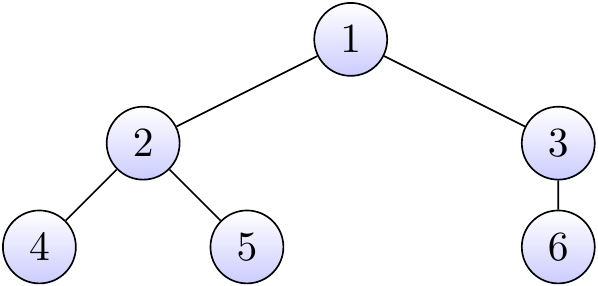
\includegraphics[width=0.9\linewidth]{tech-interview_files/figure-latex/unnamed-chunk-17-1} \caption{Some caption.}\label{fig:unnamed-chunk-17}
\end{figure}

output 6

\hypertarget{solution-39}{%
\subsection{Solution}\label{solution-39}}

\hypertarget{walkthrough-61}{%
\subsubsection{Walkthrough\textbackslash{}}\label{walkthrough-61}}

Recursively call at each node, and determine if it is a full binary tree or complete binary tree. if it is full
binary tree (left height == right height), return \((2^{h} - 1)\), else return 1 + rec(node.left) + rec(node.right)

\hypertarget{analysis-68}{%
\subsubsection{Analysis\textbackslash{}}\label{analysis-68}}

Time complexity is O(n) as every node is visited once.

\hypertarget{algorithm-70}{%
\subsubsection{Algorithm\textbackslash{}}\label{algorithm-70}}

dfs \ref{dfs}

\hypertarget{java-code-43}{%
\subsection{Java Code}\label{java-code-43}}

\begin{Shaded}
\begin{Highlighting}[]
\KeywordTok{public} \DataTypeTok{int} \FunctionTok{countNodes}\NormalTok{(}\BuiltInTok{TreeNode}\NormalTok{ root) \{}
    \KeywordTok{if}\NormalTok{(root == }\KeywordTok{null}\NormalTok{) \{}
        \KeywordTok{return} \DecValTok{0}\NormalTok{;}
\NormalTok{    \}}
    \DataTypeTok{int}\NormalTok{ lHeight = }\DecValTok{0}\NormalTok{, rHeight = }\DecValTok{0}\NormalTok{;}

    \KeywordTok{for}\NormalTok{ (}\BuiltInTok{TreeNode}\NormalTok{ node = root; node != }\KeywordTok{null}\NormalTok{; node = node.}\FunctionTok{left}\NormalTok{, lHeight++);}
    \KeywordTok{for}\NormalTok{ (}\BuiltInTok{TreeNode}\NormalTok{ node = root; node != }\KeywordTok{null}\NormalTok{; node = node.}\FunctionTok{right}\NormalTok{, rHeight++);}

    \KeywordTok{if}\NormalTok{ (lHeight == rHeight) \{}
        \CommentTok{/*}
\CommentTok{        * full binary tree}
\CommentTok{        * 2^leftNum - 1}
\CommentTok{        */}
        \KeywordTok{return}\NormalTok{ (}\DecValTok{1}\NormalTok{ << lHeight) - }\DecValTok{1}\NormalTok{;}
\NormalTok{    \} }\KeywordTok{else}\NormalTok{ \{}
        \KeywordTok{return} \DecValTok{1}\NormalTok{ + }\FunctionTok{countNodes}\NormalTok{(root.}\FunctionTok{left}\NormalTok{) + }\FunctionTok{countNodes}\NormalTok{(root.}\FunctionTok{right}\NormalTok{);}
\NormalTok{    \}}
\NormalTok{\}}
\end{Highlighting}
\end{Shaded}

\hypertarget{distance-of-a-node-from-the-root-firebase-level-3}{%
\section{Distance of a node from the root / Firebase / Level 3}\label{distance-of-a-node-from-the-root-firebase-level-3}}

\hypertarget{description-58}{%
\subsection{Description}\label{description-58}}

Given the root of a Binary Tree and an integer that represents the data value of a TreeNode present in the tree,
write a method - pathLengthFromRoot that returns the distance between the root and that node. You can assume that the
given key exists in the tree. The distance is defined as the minimum number of nodes that must be traversed to reach
the target node.

\hypertarget{example-56}{%
\subsection{Example}\label{example-56}}

\begin{figure}
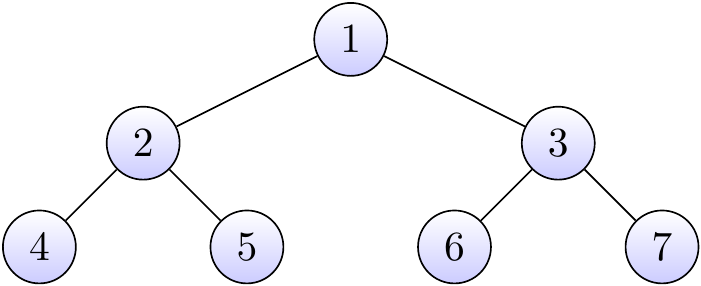
\includegraphics[width=0.9\linewidth]{tech-interview_files/figure-latex/unnamed-chunk-18-1} \caption{Some caption.}\label{fig:unnamed-chunk-18}
\end{figure}

pathLengthFromRoot(root,5) = 3

pathLengthFromRoot(root,1) = 1

pathLengthFromRoot(root,3) = 2

\hypertarget{solution-40}{%
\subsection{Solution}\label{solution-40}}

\hypertarget{walkthrough-62}{%
\subsubsection{Walkthrough\textbackslash{}}\label{walkthrough-62}}

Have a global variable of ArrayList to remember the path. Create a helper function to recursively traverse the tree.
If the target does not lie either in the left or right subtree of the current node.Thus, remove current node's value
from trace list.

\hypertarget{analysis-69}{%
\subsubsection{Analysis\textbackslash{}}\label{analysis-69}}

Time complexity is O(n) as every node is visited once.

\hypertarget{algorithm-71}{%
\subsubsection{Algorithm\textbackslash{}}\label{algorithm-71}}

backtrack \ref{backtrack}, dfs \ref{dfs}

\hypertarget{java-code-44}{%
\subsection{Java Code}\label{java-code-44}}

\begin{Shaded}
\begin{Highlighting}[]
\BuiltInTok{List}\NormalTok{<}\BuiltInTok{TreeNode}\NormalTok{> trace = }\KeywordTok{new} \BuiltInTok{ArrayList}\NormalTok{<>();}

\DataTypeTok{int} \FunctionTok{pathLengthFromRoot}\NormalTok{(}\BuiltInTok{TreeNode}\NormalTok{ root, }\DataTypeTok{int}\NormalTok{ target) \{}
\NormalTok{    path.}\FunctionTok{clear}\NormalTok{();}

    \DataTypeTok{boolean}\NormalTok{ result = }\FunctionTok{backtrack}\NormalTok{(root, target);}

    \KeywordTok{if}\NormalTok{(result) \{}
        \KeywordTok{return}\NormalTok{ trace.}\FunctionTok{size}\NormalTok{();}
\NormalTok{    \} }\KeywordTok{else}\NormalTok{ \{}
        \KeywordTok{return} \DecValTok{0}\NormalTok{;}
\NormalTok{    \}}
\NormalTok{\}}

\DataTypeTok{boolean} \FunctionTok{backtrack}\NormalTok{(}\BuiltInTok{TreeNode}\NormalTok{ root, }\DataTypeTok{int}\NormalTok{ target) \{}
\NormalTok{    trace.}\FunctionTok{add}\NormalTok{(root);}

    \KeywordTok{if}\NormalTok{(root == }\KeywordTok{null}\NormalTok{) \{}
        \KeywordTok{return} \KeywordTok{false}\NormalTok{;}
\NormalTok{    \}}
    \KeywordTok{if}\NormalTok{(root.}\FunctionTok{data}\NormalTok{ == target) \{}
        \CommentTok{//found the node}
        \KeywordTok{return} \KeywordTok{true}\NormalTok{;}
\NormalTok{    \}}

    \KeywordTok{if}\NormalTok{(}\FunctionTok{backtrack}\NormalTok{(root.}\FunctionTok{left}\NormalTok{, target) || }\FunctionTok{backtrack}\NormalTok{(root.}\FunctionTok{right}\NormalTok{, target) ) \{}
        \KeywordTok{return} \KeywordTok{true}\NormalTok{;}
\NormalTok{    \}}

    \CommentTok{//not in current path, backtrack}
\NormalTok{    trace.}\FunctionTok{remove}\NormalTok{(path.}\FunctionTok{size}\NormalTok{() - }\DecValTok{1}\NormalTok{);}
    \KeywordTok{return} \KeywordTok{false}\NormalTok{;}
\NormalTok{\}}
\end{Highlighting}
\end{Shaded}

\hypertarget{path-sum-leet-code-112-easy}{%
\section{Path Sum / Leet Code 112 / Easy}\label{path-sum-leet-code-112-easy}}

\hypertarget{description-59}{%
\subsection{Description}\label{description-59}}

Given a binary tree and a sum, determine if the tree has a root-to-leaf path such that adding up all the values
along the path equals the given sum.

\hypertarget{example-57}{%
\subsection{Example}\label{example-57}}

\begin{figure}
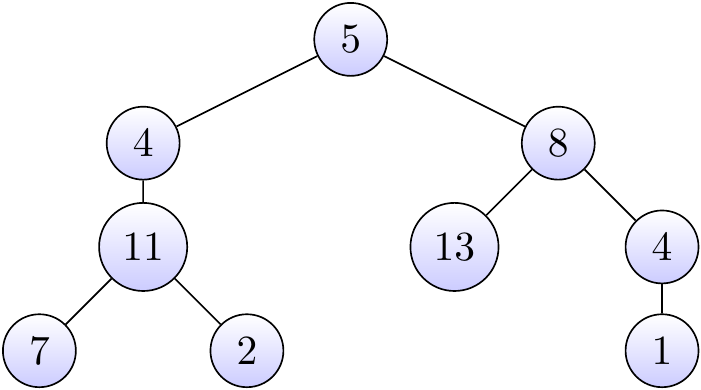
\includegraphics[width=0.9\linewidth]{tech-interview_files/figure-latex/unnamed-chunk-19-1} \caption{Some caption.}\label{fig:unnamed-chunk-19}
\end{figure}

Given the below binary tree and sum = 22, return true, as there exist a root-to-leaf path \(5->4->11->2\) which sum
is 22.

\hypertarget{solution-41}{%
\subsection{Solution}\label{solution-41}}

\hypertarget{walkthrough-63}{%
\subsubsection{Walkthrough\textbackslash{}}\label{walkthrough-63}}

Has a variable to remember accumulated sum and recursively call on its left and right subtree. \textbf{Return}
the result if and only if the accumulated sum equals to target sum or accumulate result with logical OR operator
also only when traversal reach to leaf node.

\hypertarget{analysis-70}{%
\subsubsection{Analysis\textbackslash{}}\label{analysis-70}}

Time complexity is O(n) as every node is visited once.

\hypertarget{algorithm-72}{%
\subsubsection{Algorithm\textbackslash{}}\label{algorithm-72}}

dfs \ref{dfs}

\hypertarget{java-code-45}{%
\subsection{Java Code}\label{java-code-45}}

\begin{Shaded}
\begin{Highlighting}[]
\KeywordTok{public} \DataTypeTok{boolean} \FunctionTok{hasPathSum}\NormalTok{(}\BuiltInTok{TreeNode}\NormalTok{ root, }\DataTypeTok{int}\NormalTok{ sum) \{}
    \KeywordTok{return} \FunctionTok{hasPathSum}\NormalTok{(root, }\DecValTok{0}\NormalTok{, sum);}
\NormalTok{\}}

\KeywordTok{public} \DataTypeTok{boolean} \FunctionTok{hasPathSum}\NormalTok{(}\BuiltInTok{TreeNode}\NormalTok{ root, }\DataTypeTok{int}\NormalTok{ current, }\DataTypeTok{int}\NormalTok{ target) \{}
    \KeywordTok{if}\NormalTok{ (root == }\KeywordTok{null}\NormalTok{) \{}
        \KeywordTok{return} \KeywordTok{false}\NormalTok{;}
\NormalTok{    \}}

\NormalTok{    current += root.}\FunctionTok{val}\NormalTok{;}

    \KeywordTok{if}\NormalTok{ (root.}\FunctionTok{left}\NormalTok{ == }\KeywordTok{null}\NormalTok{ && root.}\FunctionTok{right}\NormalTok{ == }\KeywordTok{null}\NormalTok{) \{}
        \KeywordTok{return}\NormalTok{ current == target;}
\NormalTok{    \} }\KeywordTok{else}\NormalTok{ \{}
        \KeywordTok{return} \FunctionTok{hasPathSum}\NormalTok{(root.}\FunctionTok{left}\NormalTok{, current, target) || }\FunctionTok{hasPathSum}\NormalTok{(root.}\FunctionTok{right}\NormalTok{, current, target);}
\NormalTok{    \}}
\NormalTok{\}}
\end{Highlighting}
\end{Shaded}

\hypertarget{path-sum-ii-leet-code-113-medium}{%
\section{Path Sum II / Leet Code 113 / Medium}\label{path-sum-ii-leet-code-113-medium}}

\hypertarget{description-60}{%
\subsection{Description}\label{description-60}}

Given a binary tree and a sum, find all root-to-leaf paths where each path's sum equals the given sum.

\hypertarget{example-58}{%
\subsection{Example}\label{example-58}}

\begin{figure}
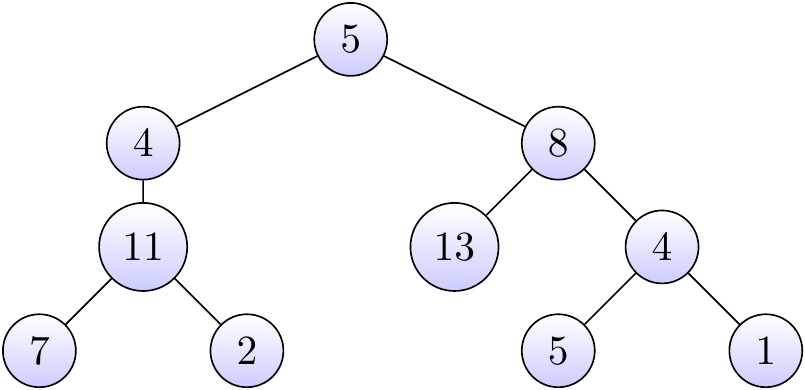
\includegraphics[width=0.9\linewidth]{tech-interview_files/figure-latex/unnamed-chunk-20-1} \caption{Some caption.}\label{fig:unnamed-chunk-20}
\end{figure}

Given the below binary tree and sum = 22, return:

\begin{verbatim}
[
    [5,4,11,2],
    [5,8,4,5]
]
\end{verbatim}

\hypertarget{solution-42}{%
\subsection{Solution}\label{solution-42}}

\hypertarget{walkthrough-64}{%
\subsubsection{Walkthrough\textbackslash{}}\label{walkthrough-64}}

Additional list is needed to keep track current path: adding current node on entering and removing (current) node on
exiting. Remember and \textbf{return} the list if and only if current sum equals to target sum for leaf nodes.
Need to remove the node list to back track also to help us locate more path in the tree.

\hypertarget{analysis-71}{%
\subsubsection{Analysis\textbackslash{}}\label{analysis-71}}

Time complexity is O(n) as every node is visited once.

\hypertarget{algorithm-73}{%
\subsubsection{Algorithm\textbackslash{}}\label{algorithm-73}}

backtrack \ref{backtrack}, dfs \ref{dfs}

\hypertarget{java-code-46}{%
\subsection{Java Code}\label{java-code-46}}

\begin{Shaded}
\begin{Highlighting}[]
\KeywordTok{public} \BuiltInTok{List}\NormalTok{<}\BuiltInTok{List}\NormalTok{<}\BuiltInTok{Integer}\NormalTok{>> }\FunctionTok{pathSum}\NormalTok{(}\BuiltInTok{TreeNode}\NormalTok{ root, }\DataTypeTok{int}\NormalTok{ sum) \{}
    \BuiltInTok{List}\NormalTok{<}\BuiltInTok{List}\NormalTok{<}\BuiltInTok{Integer}\NormalTok{>> result = }\KeywordTok{new} \BuiltInTok{LinkedList}\NormalTok{<>();}
    \BuiltInTok{List}\NormalTok{<}\BuiltInTok{Integer}\NormalTok{> trace = }\KeywordTok{new} \BuiltInTok{LinkedList}\NormalTok{<>();}
    \FunctionTok{backtrack}\NormalTok{(root, }\DecValTok{0}\NormalTok{, sum, result, trace);}
    \KeywordTok{return}\NormalTok{ result;}
\NormalTok{\}}
\KeywordTok{private} \DataTypeTok{void} \FunctionTok{backtrack}\NormalTok{(}\BuiltInTok{TreeNode}\NormalTok{ root, }\DataTypeTok{int}\NormalTok{ current, }\DataTypeTok{int}\NormalTok{ target, }\BuiltInTok{List}\NormalTok{<}\BuiltInTok{List}\NormalTok{<}\BuiltInTok{Integer}\NormalTok{>> result, }\BuiltInTok{List}\NormalTok{<}\BuiltInTok{Integer}\NormalTok{> trace) \{}
    \KeywordTok{if}\NormalTok{ (root == }\KeywordTok{null}\NormalTok{) \{}
        \KeywordTok{return}\NormalTok{;}
\NormalTok{    \}}
\NormalTok{    trace.}\FunctionTok{add}\NormalTok{(root.}\FunctionTok{val}\NormalTok{);}
\NormalTok{    current += root.}\FunctionTok{val}\NormalTok{;}

    \CommentTok{//leaf node}
    \KeywordTok{if}\NormalTok{ (root.}\FunctionTok{left}\NormalTok{ == }\KeywordTok{null}\NormalTok{ && root.}\FunctionTok{right}\NormalTok{ == }\KeywordTok{null}\NormalTok{ && current == target) \{}
        \CommentTok{//to copy the valid list}
\NormalTok{        result.}\FunctionTok{add}\NormalTok{(}\KeywordTok{new} \BuiltInTok{LinkedList}\NormalTok{<>(trace));}
        \KeywordTok{return}\NormalTok{;}
\NormalTok{    \}}

    \CommentTok{//otherwise - intermediate nodes}
    \KeywordTok{if}\NormalTok{ (root.}\FunctionTok{left}\NormalTok{ != }\KeywordTok{null}\NormalTok{) \{}
        \FunctionTok{pathSum}\NormalTok{(root.}\FunctionTok{left}\NormalTok{, current, target, result, trace);}

        \CommentTok{//clean up last inserted left node to back track one step}
\NormalTok{        trace.}\FunctionTok{remove}\NormalTok{(trace.}\FunctionTok{size}\NormalTok{() - }\DecValTok{1}\NormalTok{);}
\NormalTok{    \}}
    \KeywordTok{if}\NormalTok{ (root.}\FunctionTok{right}\NormalTok{ != }\KeywordTok{null}\NormalTok{) \{}
        \FunctionTok{pathSum}\NormalTok{(root.}\FunctionTok{right}\NormalTok{, current, target, result, trace);}

        \CommentTok{//clean up last inserted right node to back track one step}
\NormalTok{        trace.}\FunctionTok{remove}\NormalTok{(trace.}\FunctionTok{size}\NormalTok{() - }\DecValTok{1}\NormalTok{);}
\NormalTok{    \}}
\NormalTok{\}}
\end{Highlighting}
\end{Shaded}

\hypertarget{path-sum-iii-leet-code-437-easy}{%
\section{Path Sum III / Leet Code 437 / Easy}\label{path-sum-iii-leet-code-437-easy}}

\hypertarget{description-61}{%
\subsection{Description}\label{description-61}}

You are given a binary tree in which each node contains an integer value.

Find the number of paths that sum to a given value.

The path does not need to start or end at the root or a leaf, but it must go downwards (traveling only from parent nodes to child nodes).

The tree has no more than 1,000 nodes and the values are in the range -1,000,000 to 1,000,000.
\#\#\# Example

\begin{figure}
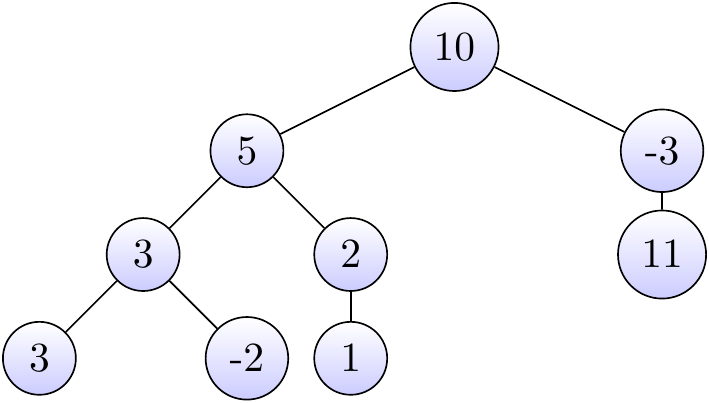
\includegraphics[width=0.9\linewidth]{tech-interview_files/figure-latex/unnamed-chunk-21-1} \caption{Some caption.}\label{fig:unnamed-chunk-21}
\end{figure}

sum = 8, Return 3. The paths that sum to 8 are:

\begin{verbatim}
1. 5 -> 3
2. 5 -> 2 -> 1
3. -3 -> 11
\end{verbatim}

\hypertarget{solution-43}{%
\subsection{Solution}\label{solution-43}}

\hypertarget{walkthrough-65}{%
\subsubsection{Walkthrough\textbackslash{}}\label{walkthrough-65}}

Continue the recursive on left and right subtrees and \textbf{do not return} when accumulated sum equals to the
target sum. Use a length-1 array to keep track the count of path number in the recursive. We should consider both
cases to include root and exlude root. For instance, if there is a tree {[}1,-2,1,-1{]} and taget sum is -1. There
are four paths combined :

\begin{verbatim}
1. [1,-2]
2. [-2,1]
3. [-1]
4. [1,-2,1,-1]
\end{verbatim}

In addition, we need to store accumulated count across recursive function calls. Thus, data type cannot be Immutable,
since each arithmetic operation would create another object. Thus, we need to have a mutable variable that exists
across each stack frame:

\begin{itemize}
\tightlist
\item
  Have a int{[}1{]} to store the accumulated count.
\item
  Have a wrapper object to reset the value towards computation.
\item
  Have a shared variable declared for this purpose.
\end{itemize}

\hypertarget{analysis-72}{%
\subsubsection{Analysis\textbackslash{}}\label{analysis-72}}

Time complexity is O(n) as every node is visited once.

\hypertarget{algorithm-74}{%
\subsubsection{Algorithm\textbackslash{}}\label{algorithm-74}}

dfs \ref{dfs}

\hypertarget{java-code-47}{%
\subsection{Java Code}\label{java-code-47}}

\begin{Shaded}
\begin{Highlighting}[]
\DataTypeTok{int}\NormalTok{ count = }\DecValTok{0}\NormalTok{;}
\KeywordTok{public} \DataTypeTok{int} \FunctionTok{pathSum}\NormalTok{(}\BuiltInTok{TreeNode}\NormalTok{ root, }\DataTypeTok{int}\NormalTok{ sum) \{}
    \FunctionTok{helperSum}\NormalTok{(root, }\DecValTok{0}\NormalTok{, sum);}
    \KeywordTok{return}\NormalTok{ count;}
\NormalTok{\}}
\KeywordTok{private} \DataTypeTok{void} \FunctionTok{helperSum}\NormalTok{(}\BuiltInTok{TreeNode}\NormalTok{ root, }\DataTypeTok{int}\NormalTok{ current, }\DataTypeTok{int}\NormalTok{ target) \{}
    \KeywordTok{if}\NormalTok{ (root == }\KeywordTok{null}\NormalTok{) \{}
        \KeywordTok{return}\NormalTok{;}
\NormalTok{    \}}
    \CommentTok{// root included}
    \FunctionTok{helper}\NormalTok{(root, current, target);}
    \CommentTok{// root excluded}
    \FunctionTok{helperSum}\NormalTok{(root.}\FunctionTok{left}\NormalTok{, current, target);}
    \FunctionTok{helperSum}\NormalTok{(root.}\FunctionTok{right}\NormalTok{, current, target);}
\NormalTok{\}}
\KeywordTok{private} \DataTypeTok{void} \FunctionTok{helper}\NormalTok{(}\BuiltInTok{TreeNode}\NormalTok{ root, }\DataTypeTok{int}\NormalTok{ current, }\DataTypeTok{int}\NormalTok{ target) \{}
    \KeywordTok{if}\NormalTok{ (root == }\KeywordTok{null}\NormalTok{) \{}
        \KeywordTok{return}\NormalTok{;}
\NormalTok{    \}}
\NormalTok{    current += root.}\FunctionTok{val}\NormalTok{;}
    \KeywordTok{if}\NormalTok{ (current == target) \{}
\NormalTok{        count++;}
        \CommentTok{// do not return.}
\NormalTok{    \}}
    \FunctionTok{helper}\NormalTok{(root.}\FunctionTok{left}\NormalTok{, current, target);}
    \FunctionTok{helper}\NormalTok{(root.}\FunctionTok{right}\NormalTok{, current, target);}
\NormalTok{\}}
\end{Highlighting}
\end{Shaded}

\hypertarget{binary-tree-preorder-traversal-leet-code-144-medium}{%
\section{Binary Tree Preorder Traversal / Leet Code 144 / Medium}\label{binary-tree-preorder-traversal-leet-code-144-medium}}

\label{sec:depth_first_preorder}

\hypertarget{description-62}{%
\subsection{Description}\label{description-62}}

Given a binary tree, return the preorder traversal of its nodes' values.

\hypertarget{example-59}{%
\subsection{Example}\label{example-59}}

\begin{figure}
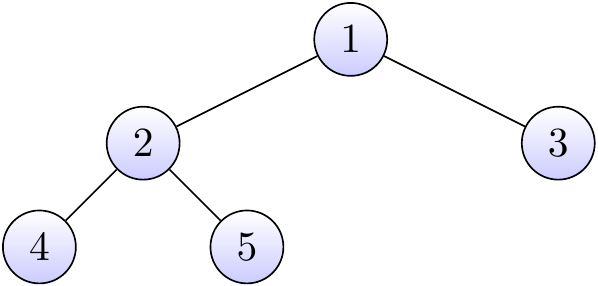
\includegraphics[width=0.9\linewidth]{tech-interview_files/figure-latex/unnamed-chunk-22-1} \caption{Some caption.}\label{fig:unnamed-chunk-22}
\end{figure}

Output: {[}1,2,4,5,3{]}

\hypertarget{solution---iterative-i}{%
\subsection{Solution - Iterative I}\label{solution---iterative-i}}

\hypertarget{walkthrough-66}{%
\subsubsection{Walkthrough\textbackslash{}}\label{walkthrough-66}}

For iterative solution, use a stack to store the root node that will be used to retrieve root.right for later use. For
initial loop condiition, be sure to include (root != null) to make sure loop starts since stack initially is empty.

\hypertarget{analysis-73}{%
\subsubsection{Analysis\textbackslash{}}\label{analysis-73}}

Time complexity is O(n) as every node is visited once.
\#\#\#\# Algorithm\textbackslash{}

\hypertarget{java-code---iterative-i}{%
\subsection{Java Code - Iterative I}\label{java-code---iterative-i}}

\begin{Shaded}
\begin{Highlighting}[]
\KeywordTok{public} \BuiltInTok{List}\NormalTok{<}\BuiltInTok{Integer}\NormalTok{> }\FunctionTok{preorderTraversal}\NormalTok{(}\BuiltInTok{TreeNode}\NormalTok{ root) \{}
    \BuiltInTok{List}\NormalTok{<}\BuiltInTok{Integer}\NormalTok{> result = }\KeywordTok{new} \BuiltInTok{ArrayList}\NormalTok{<>();}
    \CommentTok{//stack is used to store the root node that will be used access root.right later}
    \BuiltInTok{Stack}\NormalTok{<}\BuiltInTok{TreeNode}\NormalTok{> stack = }\KeywordTok{new} \BuiltInTok{Stack}\NormalTok{<>();}

    \KeywordTok{while}\NormalTok{(!stack.}\FunctionTok{isEmpty}\NormalTok{() || root != }\KeywordTok{null}\NormalTok{) \{}
        \KeywordTok{if}\NormalTok{(root != }\KeywordTok{null}\NormalTok{) \{}
\NormalTok{            stack.}\FunctionTok{push}\NormalTok{(root);}
\NormalTok{            result.}\FunctionTok{add}\NormalTok{(root.}\FunctionTok{val}\NormalTok{); }\CommentTok{// Add before going to children}
\NormalTok{            root = root.}\FunctionTok{left}\NormalTok{;}
\NormalTok{        \} }\KeywordTok{else}\NormalTok{ \{}
\NormalTok{            root = stack.}\FunctionTok{pop}\NormalTok{().}\FunctionTok{right}\NormalTok{;}
\NormalTok{        \}}
\NormalTok{    \}}
    \KeywordTok{return}\NormalTok{ result;}
\NormalTok{\}}
\end{Highlighting}
\end{Shaded}

\hypertarget{solution---iterative-ii}{%
\subsection{Solution - Iterative II}\label{solution---iterative-ii}}

\hypertarget{walkthrough-67}{%
\subsubsection{Walkthrough\textbackslash{}}\label{walkthrough-67}}

To convert an inherently recursive procedures to iterative, we need an explicit stack, and do following
while the stack is not empty:

\begin{itemize}
\tightlist
\item
  Pop an item from stack and process it.
\item
  Push \textbf{right child} of popped item to stack
\item
  Push \textbf{left child} of popped item to stack
\end{itemize}

Since stack is a LIFO, when the right child node is pushed before the left child node to a stack, the left
child node would be processed before the right child node.

\hypertarget{analysis-74}{%
\subsubsection{Analysis\textbackslash{}}\label{analysis-74}}

Time complexity is O(n) as every node is visited once.

\hypertarget{algorithm-75}{%
\subsubsection{Algorithm\textbackslash{}}\label{algorithm-75}}

\hypertarget{java-code---iterative-ii}{%
\subsection{Java Code - Iterative II}\label{java-code---iterative-ii}}

\begin{Shaded}
\begin{Highlighting}[]
\KeywordTok{public} \BuiltInTok{List}\NormalTok{<}\BuiltInTok{Integer}\NormalTok{> }\FunctionTok{preorderTraversal}\NormalTok{(}\BuiltInTok{TreeNode}\NormalTok{ root) \{}
    \BuiltInTok{List}\NormalTok{<}\BuiltInTok{Integer}\NormalTok{> result = }\KeywordTok{new} \BuiltInTok{ArrayList}\NormalTok{<>();}
    \CommentTok{//stack is used to store the root node that will be used access root.right later}
    \BuiltInTok{Stack}\NormalTok{<}\BuiltInTok{TreeNode}\NormalTok{> stack = }\KeywordTok{new} \BuiltInTok{Stack}\NormalTok{<>();}

    \KeywordTok{if}\NormalTok{ (root == }\KeywordTok{null}\NormalTok{) \{}
        \KeywordTok{return}\NormalTok{ result;}
\NormalTok{    \}}
\NormalTok{    stack.}\FunctionTok{push}\NormalTok{(root);}

    \KeywordTok{while}\NormalTok{ (!stack.}\FunctionTok{empty}\NormalTok{()) \{}
        \BuiltInTok{Node}\NormalTok{ node = nodeStack.}\FunctionTok{pop}\NormalTok{();}
\NormalTok{        result.}\FunctionTok{add}\NormalTok{(node.}\FunctionTok{val}\NormalTok{);}

        \CommentTok{// Push the RIGHT child of the popped node to stack}
        \KeywordTok{if}\NormalTok{ (node.}\FunctionTok{right}\NormalTok{ != }\KeywordTok{null}\NormalTok{) \{}
\NormalTok{            stack.}\FunctionTok{push}\NormalTok{(node.}\FunctionTok{right}\NormalTok{);}
\NormalTok{        \}}
        \CommentTok{// Push the LEFT child of the popped node to stack}
        \KeywordTok{if}\NormalTok{ (node.}\FunctionTok{left}\NormalTok{ != }\KeywordTok{null}\NormalTok{) \{}
\NormalTok{            stack.}\FunctionTok{push}\NormalTok{(node.}\FunctionTok{left}\NormalTok{);}
\NormalTok{        \}}
\NormalTok{    \}}

    \KeywordTok{return}\NormalTok{ result;}
\NormalTok{\}}
\end{Highlighting}
\end{Shaded}

\hypertarget{solution---recursive-1}{%
\subsection{Solution - Recursive}\label{solution---recursive-1}}

\hypertarget{walkthrough-68}{%
\subsubsection{Walkthrough\textbackslash{}}\label{walkthrough-68}}

For recursive implementation, do the following step

\begin{itemize}
\tightlist
\item
  To process data at current node
\item
  Recursively invoke left child node.
\item
  Recursively invoke right child node.
\end{itemize}

\hypertarget{analysis-75}{%
\subsubsection{Analysis\textbackslash{}}\label{analysis-75}}

Time complexity is O(n) as every node is visited once. Auxiliary Space is O(1) if we do not consider the size of stacks
for function calls, otherwise O(n).

\hypertarget{algorithm-76}{%
\subsubsection{Algorithm\textbackslash{}}\label{algorithm-76}}

dfs \ref{dfs}

\hypertarget{java-code---recursive-1}{%
\subsection{Java Code - Recursive}\label{java-code---recursive-1}}

\begin{Shaded}
\begin{Highlighting}[]
\KeywordTok{public} \BuiltInTok{List}\NormalTok{<}\BuiltInTok{Integer}\NormalTok{> }\FunctionTok{preorderTraversal}\NormalTok{(}\BuiltInTok{TreeNode}\NormalTok{ root) \{}
    \BuiltInTok{List}\NormalTok{<}\BuiltInTok{Integer}\NormalTok{> result = }\KeywordTok{new} \BuiltInTok{ArrayList}\NormalTok{<>();}
    \FunctionTok{traversalHelper}\NormalTok{(root, result);}

    \KeywordTok{return}\NormalTok{ result;}
\NormalTok{\}}

\KeywordTok{public} \DataTypeTok{void} \FunctionTok{traversalHelper}\NormalTok{(}\BuiltInTok{TreeNode}\NormalTok{ root, }\BuiltInTok{List}\NormalTok{<}\BuiltInTok{Integer}\NormalTok{> list) \{}
    \KeywordTok{if}\NormalTok{(root == }\KeywordTok{null}\NormalTok{) \{}
        \KeywordTok{return}\NormalTok{;}
\NormalTok{    \}}

\NormalTok{    list.}\FunctionTok{add}\NormalTok{(root.}\FunctionTok{val}\NormalTok{);}
    \FunctionTok{traversalHelper}\NormalTok{(root.}\FunctionTok{left}\NormalTok{, list);}
    \FunctionTok{traversalHelper}\NormalTok{(root.}\FunctionTok{right}\NormalTok{, list);}
\NormalTok{\}}
\end{Highlighting}
\end{Shaded}

\hypertarget{binary-tree-inorder-traversal-leet-code-94-medium}{%
\section{Binary Tree Inorder Traversal / Leet Code 94 / Medium}\label{binary-tree-inorder-traversal-leet-code-94-medium}}

\label{sec:depth_first_inorder}

\hypertarget{description-63}{%
\subsection{Description}\label{description-63}}

Given a binary tree, return the inorder traversal of its nodes' values.

\hypertarget{example-60}{%
\subsection{Example}\label{example-60}}

\begin{figure}
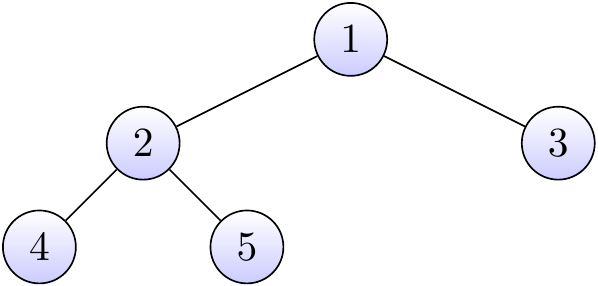
\includegraphics[width=0.9\linewidth]{tech-interview_files/figure-latex/unnamed-chunk-23-1} \caption{Some caption.}\label{fig:unnamed-chunk-23}
\end{figure}

Output: {[}4, 2, 5, 1, 3{]}

\hypertarget{solution---iterative-i-1}{%
\subsection{Solution - Iterative I}\label{solution---iterative-i-1}}

\hypertarget{walkthrough-69}{%
\subsubsection{Walkthrough\textbackslash{}}\label{walkthrough-69}}

For iterative solution, use a stack to store the root node that will be used to retrieve root.right for later use. For
initial loop condiition, be sure to include (root != null) to make sure loop starts since stack initially is empty.

\hypertarget{analysis-76}{%
\subsubsection{Analysis\textbackslash{}}\label{analysis-76}}

Time complexity is O(n) as every node is visited once.

\hypertarget{algorithm-77}{%
\subsubsection{Algorithm\textbackslash{}}\label{algorithm-77}}

\hypertarget{java-code---iterative-i-1}{%
\subsection{Java Code - Iterative I}\label{java-code---iterative-i-1}}

\begin{Shaded}
\begin{Highlighting}[]
\KeywordTok{public} \BuiltInTok{List}\NormalTok{<}\BuiltInTok{Integer}\NormalTok{> }\FunctionTok{inorderTraversal}\NormalTok{(}\BuiltInTok{TreeNode}\NormalTok{ root) \{}
    \BuiltInTok{List}\NormalTok{<}\BuiltInTok{Integer}\NormalTok{> result = }\KeywordTok{new} \BuiltInTok{ArrayList}\NormalTok{<>();}
    \CommentTok{//stack is used to store the root node that will be used access root.right later}
    \BuiltInTok{Stack}\NormalTok{<}\BuiltInTok{TreeNode}\NormalTok{> stack = }\KeywordTok{new} \BuiltInTok{Stack}\NormalTok{<>();}

    \KeywordTok{while}\NormalTok{(!stack.}\FunctionTok{isEmpty}\NormalTok{() || root != }\KeywordTok{null}\NormalTok{) \{}
        \KeywordTok{if}\NormalTok{(root != }\KeywordTok{null}\NormalTok{) \{}
\NormalTok{            stack.}\FunctionTok{push}\NormalTok{(root);}
\NormalTok{            root = root.}\FunctionTok{left}\NormalTok{;}
\NormalTok{        \} }\KeywordTok{else}\NormalTok{ \{}
\NormalTok{            root = stack.}\FunctionTok{pop}\NormalTok{();}
\NormalTok{            result.}\FunctionTok{add}\NormalTok{(root.}\FunctionTok{val}\NormalTok{);}
\NormalTok{            root = root.}\FunctionTok{right}\NormalTok{;}
\NormalTok{        \}}
\NormalTok{    \}}
    \KeywordTok{return}\NormalTok{ result;}
\NormalTok{\}}
\end{Highlighting}
\end{Shaded}

\hypertarget{solution---inorder-recursive}{%
\subsection{Solution - Inorder Recursive}\label{solution---inorder-recursive}}

\hypertarget{walkthrough-70}{%
\subsubsection{Walkthrough\textbackslash{}}\label{walkthrough-70}}

For recursive implementation, do the following step

\begin{itemize}
\tightlist
\item
  Recursively invoke left child node.
\item
  To process data at current node
\item
  Recursively invoke right child node.
\end{itemize}

\hypertarget{analysis-77}{%
\subsubsection{Analysis\textbackslash{}}\label{analysis-77}}

Time complexity is O(n) as every node is visited once. Auxiliary Space is O(1) if we do not consider the size of stacks
for function calls, otherwise O(n).

\hypertarget{algorithm-78}{%
\subsubsection{Algorithm\textbackslash{}}\label{algorithm-78}}

dfs \ref{dfs}

\hypertarget{java-code---inorder-recursive}{%
\subsection{Java Code - Inorder Recursive}\label{java-code---inorder-recursive}}

\begin{Shaded}
\begin{Highlighting}[]
\KeywordTok{public} \BuiltInTok{List}\NormalTok{<}\BuiltInTok{Integer}\NormalTok{> }\FunctionTok{inorderTraversal}\NormalTok{(}\BuiltInTok{TreeNode}\NormalTok{ root) \{}
    \BuiltInTok{List}\NormalTok{<}\BuiltInTok{Integer}\NormalTok{> result = }\KeywordTok{new} \BuiltInTok{ArrayList}\NormalTok{<>();}
    \FunctionTok{traversalHelper}\NormalTok{(root, result);}

    \KeywordTok{return}\NormalTok{ result;}
\NormalTok{\}}

\KeywordTok{public} \DataTypeTok{void} \FunctionTok{traversalHelper}\NormalTok{(}\BuiltInTok{TreeNode}\NormalTok{ root, }\BuiltInTok{List}\NormalTok{<}\BuiltInTok{Integer}\NormalTok{> list) \{}
    \KeywordTok{if}\NormalTok{(root == }\KeywordTok{null}\NormalTok{) \{}
        \KeywordTok{return}\NormalTok{;}
\NormalTok{    \}}

    \FunctionTok{traversalHelper}\NormalTok{(root.}\FunctionTok{left}\NormalTok{, list);}
\NormalTok{    list.}\FunctionTok{add}\NormalTok{(root.}\FunctionTok{val}\NormalTok{);}
    \FunctionTok{traversalHelper}\NormalTok{(root.}\FunctionTok{right}\NormalTok{, list);}
\NormalTok{\}}
\end{Highlighting}
\end{Shaded}

\hypertarget{binary-tree-postorder-traversal-leet-code-145-hard}{%
\section{Binary Tree Postorder Traversal / Leet Code 145 / Hard}\label{binary-tree-postorder-traversal-leet-code-145-hard}}

\label{sec:depth_first_postorder}

\hypertarget{description-64}{%
\subsection{Description}\label{description-64}}

Given a binary tree, return the postorder traversal of its nodes' values.

\hypertarget{example-61}{%
\subsection{Example}\label{example-61}}

\begin{figure}
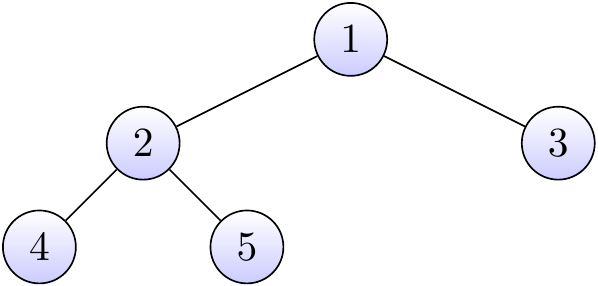
\includegraphics[width=0.9\linewidth]{tech-interview_files/figure-latex/unnamed-chunk-24-1} \caption{Some caption.}\label{fig:unnamed-chunk-24}
\end{figure}

Output: {[}4, 5, 2, 3, 1{]}

\hypertarget{solution---iterative-i-2}{%
\subsection{Solution - Iterative I}\label{solution---iterative-i-2}}

\hypertarget{walkthrough-71}{%
\subsubsection{Walkthrough\textbackslash{}}\label{walkthrough-71}}

For iterative solution, use a stack to store the root node that will be used to retrieve root.right for later use. For
initial loop condiition, be sure to include (root != null) to make sure loop starts since stack initially is empty.

\hypertarget{analysis-78}{%
\subsubsection{Analysis\textbackslash{}}\label{analysis-78}}

Time complexity is O(n) as every node is visited once.

\hypertarget{algorithm-79}{%
\subsubsection{Algorithm\textbackslash{}}\label{algorithm-79}}

\hypertarget{java-code---iterative-i-2}{%
\subsection{Java Code - Iterative I}\label{java-code---iterative-i-2}}

\begin{Shaded}
\begin{Highlighting}[]
\KeywordTok{public} \BuiltInTok{List}\NormalTok{<}\BuiltInTok{Integer}\NormalTok{> }\FunctionTok{postorderTraversal}\NormalTok{(}\BuiltInTok{TreeNode}\NormalTok{ root) \{}
    \BuiltInTok{List}\NormalTok{<}\BuiltInTok{Integer}\NormalTok{> result = }\KeywordTok{new} \BuiltInTok{ArrayList}\NormalTok{<>();}
    \CommentTok{//stack is used to store the root node that will be used access root.right later}
    \BuiltInTok{Stack}\NormalTok{<}\BuiltInTok{TreeNode}\NormalTok{> stack = }\KeywordTok{new} \BuiltInTok{Stack}\NormalTok{<>();}

    \KeywordTok{while}\NormalTok{(!stack.}\FunctionTok{isEmpty}\NormalTok{() || root != }\KeywordTok{null}\NormalTok{) \{}
        \KeywordTok{if}\NormalTok{(root != }\KeywordTok{null}\NormalTok{) \{}
\NormalTok{            stack.}\FunctionTok{push}\NormalTok{(root);}

            \CommentTok{//insert to head}
\NormalTok{            result.}\FunctionTok{add}\NormalTok{(}\DecValTok{0}\NormalTok{, root.}\FunctionTok{val}\NormalTok{);}
\NormalTok{            root = root.}\FunctionTok{right}\NormalTok{;}
\NormalTok{        \} }\KeywordTok{else}\NormalTok{ \{}
\NormalTok{            root = stack.}\FunctionTok{pop}\NormalTok{().}\FunctionTok{left}\NormalTok{;}
\NormalTok{        \}}
\NormalTok{    \}}
    \KeywordTok{return}\NormalTok{ result;}
\NormalTok{\}}
\end{Highlighting}
\end{Shaded}

\hypertarget{solution---iterative-with-two-stacks}{%
\subsection{Solution - Iterative with Two Stacks}\label{solution---iterative-with-two-stacks}}

\hypertarget{walkthrough-72}{%
\subsubsection{Walkthrough\textbackslash{}}\label{walkthrough-72}}

The idea is to push reverse postorder traversal to a stack. Once we have the reversed postorder traversal in
a stack, we can just pop all items one by one from the stack and process them; this order will be in
postorder because of the LIFO property of stacks. To get a reversed postorder elements in a stack -
the second stack is used for this purpose, this sequence is very similar to the preorder traversal. The only
difference is that the right child is visited before left child, and therefore the sequence is
``root right left'' instead of ``root left right''.

\hypertarget{analysis-79}{%
\subsubsection{Analysis\textbackslash{}}\label{analysis-79}}

Time complexity is O(n) as every node is visited once.

\hypertarget{algorithm-80}{%
\subsubsection{Algorithm\textbackslash{}}\label{algorithm-80}}

\hypertarget{java-code---iterative-with-two-stacks}{%
\subsection{Java Code - Iterative with Two Stacks}\label{java-code---iterative-with-two-stacks}}

\begin{Shaded}
\begin{Highlighting}[]
\KeywordTok{public} \BuiltInTok{List}\NormalTok{<}\BuiltInTok{Integer}\NormalTok{> }\FunctionTok{postorderTraversal}\NormalTok{(}\BuiltInTok{TreeNode}\NormalTok{ root) \{}
    \BuiltInTok{List}\NormalTok{<}\BuiltInTok{Integer}\NormalTok{> result = }\KeywordTok{new} \BuiltInTok{ArrayList}\NormalTok{<>();}

    \BuiltInTok{Stack}\NormalTok{<}\BuiltInTok{TreeNode}\NormalTok{> stack1 = }\KeywordTok{new} \BuiltInTok{Stack}\NormalTok{<>();}
    \CommentTok{//stack2 is used to store the reversed postorder elements in a stack}
    \BuiltInTok{Stack}\NormalTok{<}\BuiltInTok{TreeNode}\NormalTok{> stack2 = }\KeywordTok{new} \BuiltInTok{Stack}\NormalTok{<>();}

    \KeywordTok{if}\NormalTok{ (root == }\KeywordTok{null}\NormalTok{) \{}
        \KeywordTok{return}\NormalTok{ result;}
\NormalTok{    \}}
\NormalTok{    stack.}\FunctionTok{push}\NormalTok{(root);}

    \KeywordTok{while}\NormalTok{ (!stack1.}\FunctionTok{isEmpty}\NormalTok{()) \{}
        \CommentTok{// Pop an item from stack1 and push it to stack2}
        \BuiltInTok{TreeNode}\NormalTok{ node = stack1.}\FunctionTok{pop}\NormalTok{();}
\NormalTok{        stack2.}\FunctionTok{push}\NormalTok{(node);}

        \CommentTok{// Push LEFT child of popped item to stack1}
        \KeywordTok{if}\NormalTok{ (node.}\FunctionTok{left}\NormalTok{ != }\KeywordTok{null}\NormalTok{) \{}
\NormalTok{            stack1.}\FunctionTok{push}\NormalTok{(node.}\FunctionTok{left}\NormalTok{);}
\NormalTok{        \}}
        \CommentTok{// Push RIGHT child of popped item to stack1}
        \KeywordTok{if}\NormalTok{ (node.}\FunctionTok{right}\NormalTok{ != }\KeywordTok{null}\NormalTok{) \{}
\NormalTok{            stack1.}\FunctionTok{push}\NormalTok{(node.}\FunctionTok{right}\NormalTok{);}
\NormalTok{        \}}
\NormalTok{    \}}

    \CommentTok{//Traverse all reversed elements in second stack}
    \KeywordTok{while}\NormalTok{ (!stack2.}\FunctionTok{isEmpty}\NormalTok{()) \{}
        \BuiltInTok{TreeNode}\NormalTok{ node = stack2.}\FunctionTok{pop}\NormalTok{();}
\NormalTok{        result.}\FunctionTok{add}\NormalTok{(node.}\FunctionTok{val}\NormalTok{)}
\NormalTok{    \}}

    \KeywordTok{return}\NormalTok{ result;}
\NormalTok{    \}}
\end{Highlighting}
\end{Shaded}

\hypertarget{solution---recursive-2}{%
\subsection{Solution - Recursive}\label{solution---recursive-2}}

\hypertarget{walkthrough-73}{%
\subsubsection{Walkthrough\textbackslash{}}\label{walkthrough-73}}

For recursive implementation, do the following step

\begin{itemize}
\tightlist
\item
  Recursively invoke left child node.
\item
  Recursively invoke right child node.
\item
  To process data at current node
\end{itemize}

\hypertarget{analysis-80}{%
\subsubsection{Analysis\textbackslash{}}\label{analysis-80}}

Time complexity is O(n) as every node is visited once. Auxiliary Space is O(1) if we do not consider the size of stacks
for function calls, otherwise O(n).

\hypertarget{algorithm-81}{%
\subsubsection{Algorithm\textbackslash{}}\label{algorithm-81}}

dfs \ref{dfs}

\hypertarget{java-code---recursive-2}{%
\subsection{Java Code - Recursive}\label{java-code---recursive-2}}

\begin{Shaded}
\begin{Highlighting}[]
\KeywordTok{public} \BuiltInTok{List}\NormalTok{<}\BuiltInTok{Integer}\NormalTok{> }\FunctionTok{postorderTraversal}\NormalTok{(}\BuiltInTok{TreeNode}\NormalTok{ root) \{}
    \BuiltInTok{List}\NormalTok{<}\BuiltInTok{Integer}\NormalTok{> result = }\KeywordTok{new} \BuiltInTok{ArrayList}\NormalTok{<>();}
    \FunctionTok{traversalHelper}\NormalTok{(root, result);}

    \KeywordTok{return}\NormalTok{ result;}
\NormalTok{\}}

\KeywordTok{public} \DataTypeTok{void} \FunctionTok{traversalHelper}\NormalTok{(}\BuiltInTok{TreeNode}\NormalTok{ root, }\BuiltInTok{List}\NormalTok{<}\BuiltInTok{Integer}\NormalTok{> list) \{}
    \KeywordTok{if}\NormalTok{(root == }\KeywordTok{null}\NormalTok{) \{}
        \KeywordTok{return}\NormalTok{;}
\NormalTok{    \}}

    \FunctionTok{traversalHelper}\NormalTok{(root.}\FunctionTok{left}\NormalTok{, list);}
    \FunctionTok{traversalHelper}\NormalTok{(root.}\FunctionTok{right}\NormalTok{, list);}
\NormalTok{    list.}\FunctionTok{add}\NormalTok{(root.}\FunctionTok{val}\NormalTok{);}
\NormalTok{\}}
\end{Highlighting}
\end{Shaded}

\hypertarget{maximum-depth-of-binary-tree-leet-code-104-easy}{%
\section{Maximum Depth of Binary Tree / Leet Code 104 / Easy}\label{maximum-depth-of-binary-tree-leet-code-104-easy}}

\hypertarget{description-65}{%
\subsection{Description}\label{description-65}}

Given a binary tree, find its maximum depth.

The maximum depth is the number of nodes along the longest path from the root node down to the farthest leaf
node.

\hypertarget{example-62}{%
\subsection{Example}\label{example-62}}

\begin{figure}
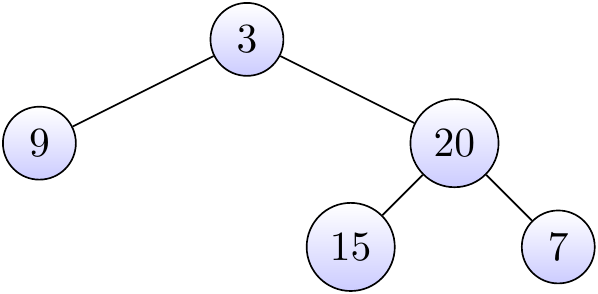
\includegraphics[width=0.9\linewidth]{tech-interview_files/figure-latex/unnamed-chunk-25-1} \caption{Some caption.}\label{fig:unnamed-chunk-25}
\end{figure}

return its depth = 3.

\hypertarget{solution-44}{%
\subsection{Solution}\label{solution-44}}

\hypertarget{walkthrough-74}{%
\subsubsection{Walkthrough\textbackslash{}}\label{walkthrough-74}}

Recursively for each level:

\begin{itemize}
\tightlist
\item
  Take the larger depth of left and right subtree.
\item
  add one for current level
\end{itemize}

\hypertarget{analysis-81}{%
\subsubsection{Analysis\textbackslash{}}\label{analysis-81}}

Time complexity is O(n) as every node is visited once.

\hypertarget{algorithm-82}{%
\subsubsection{Algorithm\textbackslash{}}\label{algorithm-82}}

recursive \ref{recursive}

\hypertarget{java-code-48}{%
\subsection{Java Code}\label{java-code-48}}

\begin{Shaded}
\begin{Highlighting}[]
\KeywordTok{public} \DataTypeTok{int} \FunctionTok{maxDepth}\NormalTok{(}\BuiltInTok{TreeNode}\NormalTok{ root) \{}
    \KeywordTok{if}\NormalTok{(root == }\KeywordTok{null}\NormalTok{) \{}
        \KeywordTok{return} \DecValTok{0}\NormalTok{;}
\NormalTok{    \}}

    \DataTypeTok{int}\NormalTok{ lHeight = }\DecValTok{0}\NormalTok{, rHeight = }\DecValTok{0}\NormalTok{;}
    \KeywordTok{if}\NormalTok{(root.}\FunctionTok{left}\NormalTok{ != }\KeywordTok{null}\NormalTok{) \{}
\NormalTok{        lHeight = }\FunctionTok{maxDepth}\NormalTok{(root.}\FunctionTok{left}\NormalTok{);}
\NormalTok{    \}}

    \KeywordTok{if}\NormalTok{(root.}\FunctionTok{right}\NormalTok{ != }\KeywordTok{null}\NormalTok{) \{}
\NormalTok{        rHeight = }\FunctionTok{maxDepth}\NormalTok{(root.}\FunctionTok{right}\NormalTok{);}
\NormalTok{    \}}

    \KeywordTok{return} \BuiltInTok{Math}\NormalTok{.}\FunctionTok{max}\NormalTok{(lHeight, rHeight) + }\DecValTok{1}\NormalTok{;}
\NormalTok{\}}
\end{Highlighting}
\end{Shaded}

\hypertarget{minimum-depth-of-binary-tree-leet-code-104-easy}{%
\section{Minimum Depth of Binary Tree / Leet Code 104 / Easy}\label{minimum-depth-of-binary-tree-leet-code-104-easy}}

\hypertarget{description-66}{%
\subsection{Description}\label{description-66}}

Given a binary tree, find its minimum depth.

The minimum depth is the number of nodes along the shortest path from the root node down to the nearest leaf
node.

\hypertarget{example-63}{%
\subsection{Example}\label{example-63}}

\begin{figure}
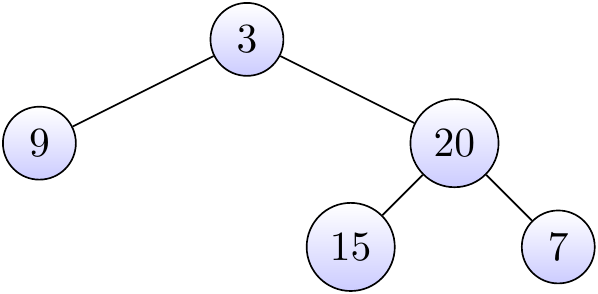
\includegraphics[width=0.9\linewidth]{tech-interview_files/figure-latex/unnamed-chunk-26-1} \caption{Some caption.}\label{fig:unnamed-chunk-26}
\end{figure}

return its minimum depth = 2.

\hypertarget{solution---recursive-3}{%
\subsection{Solution - Recursive}\label{solution---recursive-3}}

\hypertarget{walkthrough-75}{%
\subsubsection{Walkthrough\textbackslash{}}\label{walkthrough-75}}

If a node has a missing child (depth is \textbf{NOT} 0 ), then we need to drill down to the other
path to the leaf node recursively. If both nodes exist, take the minimum value out of the left and right subtree.

\hypertarget{analysis-82}{%
\subsubsection{Analysis\textbackslash{}}\label{analysis-82}}

Time complexity is O(n) as every node is visited once.

\hypertarget{algorithm-83}{%
\subsubsection{Algorithm\textbackslash{}}\label{algorithm-83}}

dfs \ref{dfs}

\hypertarget{java-code---recursive-3}{%
\subsection{Java Code - Recursive}\label{java-code---recursive-3}}

\begin{Shaded}
\begin{Highlighting}[]
\KeywordTok{public} \DataTypeTok{int} \FunctionTok{minDepth}\NormalTok{(}\BuiltInTok{TreeNode}\NormalTok{ root) \{}
    \KeywordTok{if}\NormalTok{(root == }\KeywordTok{null}\NormalTok{) \{}
        \KeywordTok{return} \DecValTok{0}\NormalTok{;}
\NormalTok{    \}}

    \KeywordTok{if}\NormalTok{(root.}\FunctionTok{left}\NormalTok{ == }\KeywordTok{null}\NormalTok{) \{}
        \CommentTok{//drill down to leaf node of the other path}
        \KeywordTok{return} \FunctionTok{minDepth}\NormalTok{(root.}\FunctionTok{right}\NormalTok{) + }\DecValTok{1}\NormalTok{;}
\NormalTok{    \} }\KeywordTok{else} \KeywordTok{if}\NormalTok{(root.}\FunctionTok{right}\NormalTok{ == }\KeywordTok{null}\NormalTok{) \{}
        \CommentTok{//drill down to leaf node of the other path}
        \KeywordTok{return} \FunctionTok{minDepth}\NormalTok{(root.}\FunctionTok{left}\NormalTok{) + }\DecValTok{1}\NormalTok{;}
\NormalTok{    \} }\KeywordTok{else}\NormalTok{ \{}
        \KeywordTok{return} \BuiltInTok{Math}\NormalTok{.}\FunctionTok{min}\NormalTok{(}\FunctionTok{minDepth}\NormalTok{(root.}\FunctionTok{left}\NormalTok{), }\FunctionTok{minDepth}\NormalTok{(root.}\FunctionTok{right}\NormalTok{)) + }\DecValTok{1}\NormalTok{;}
\NormalTok{    \}}
\NormalTok{\}}
\end{Highlighting}
\end{Shaded}

\hypertarget{solution---iterative-bfs}{%
\subsection{Solution - Iterative BFS}\label{solution---iterative-bfs}}

\hypertarget{walkthrough-76}{%
\subsubsection{Walkthrough\textbackslash{}}\label{walkthrough-76}}

Iterative: With BFS strategy, use two queues. One for current level and the other for next level.

\begin{itemize}
\tightlist
\item
  While traversing the currentLevel queue, add left and right children to the nextLevel queue.
\item
  If currentLevel is empty, switch to nextLevel by currentLevel=nextLevel and nextLevel = new Queue();
  Also, increment depth by 1
\end{itemize}

\hypertarget{analysis-83}{%
\subsubsection{Analysis\textbackslash{}}\label{analysis-83}}

Time complexity is O(n) as every node is visited once.

\hypertarget{algorithm-84}{%
\subsubsection{Algorithm\textbackslash{}}\label{algorithm-84}}

bfs \ref{bfs}

\hypertarget{java-code---iterative-bfs}{%
\subsection{Java Code - Iterative BFS}\label{java-code---iterative-bfs}}

\begin{Shaded}
\begin{Highlighting}[]
\KeywordTok{public} \DataTypeTok{int} \FunctionTok{minDepth}\NormalTok{(}\BuiltInTok{TreeNode}\NormalTok{ root) \{}
    \KeywordTok{if}\NormalTok{(root == }\KeywordTok{null}\NormalTok{) \{}
        \KeywordTok{return} \DecValTok{0}\NormalTok{;}
\NormalTok{    \}}

    \BuiltInTok{Queue}\NormalTok{<}\BuiltInTok{TreeNode}\NormalTok{> currentLevel = }\KeywordTok{new} \BuiltInTok{LinkedList}\NormalTok{<>();}
    \BuiltInTok{Queue}\NormalTok{<}\BuiltInTok{TreeNode}\NormalTok{> nextLevel = }\KeywordTok{new} \BuiltInTok{LinkedList}\NormalTok{<>();}

\NormalTok{    currentLevel.}\FunctionTok{offer}\NormalTok{(root);}
    \DataTypeTok{int}\NormalTok{ depth = }\DecValTok{1}\NormalTok{;}

    \KeywordTok{while}\NormalTok{(!currentLevel.}\FunctionTok{isEmpty}\NormalTok{()) \{}
        \BuiltInTok{TreeNode}\NormalTok{ node = currentLevel.}\FunctionTok{poll}\NormalTok{();}

        \KeywordTok{if}\NormalTok{(node.}\FunctionTok{left}\NormalTok{ == }\KeywordTok{null}\NormalTok{ && node.}\FunctionTok{right}\NormalTok{ == }\KeywordTok{null}\NormalTok{) \{}
            \KeywordTok{return}\NormalTok{ depth;}
\NormalTok{        \}}

        \KeywordTok{if}\NormalTok{(node.}\FunctionTok{left}\NormalTok{ != }\KeywordTok{null}\NormalTok{) \{}
\NormalTok{            nextLevel.}\FunctionTok{offer}\NormalTok{(node.}\FunctionTok{left}\NormalTok{);}
\NormalTok{        \}}

        \KeywordTok{if}\NormalTok{(node.}\FunctionTok{right}\NormalTok{ != }\KeywordTok{null}\NormalTok{) \{}
\NormalTok{            nextLevel.}\FunctionTok{offer}\NormalTok{(node.}\FunctionTok{right}\NormalTok{);}
\NormalTok{        \}}

        \CommentTok{//go to children level by swapping queues, increase depth}
        \KeywordTok{if}\NormalTok{(currentLevel.}\FunctionTok{isEmpty}\NormalTok{()) \{}
\NormalTok{            currentLevel = nextLevel;}
\NormalTok{            nextLevel = }\KeywordTok{new} \BuiltInTok{LinkedList}\NormalTok{<>();}
\NormalTok{            depth++;}
\NormalTok{        \}}
\NormalTok{    \}}

    \KeywordTok{return}\NormalTok{ depth;}
\NormalTok{\}}
\end{Highlighting}
\end{Shaded}

\hypertarget{count-univalue-subtrees-leet-code-250-medium}{%
\section{Count Univalue Subtrees / Leet Code 250 / Medium}\label{count-univalue-subtrees-leet-code-250-medium}}

\hypertarget{description-67}{%
\subsection{Description}\label{description-67}}

Given a binary tree, count the number of uni-value subtrees. A Uni-value subtree means all nodes of the
subtree have the same value.

\hypertarget{example-64}{%
\subsection{Example}\label{example-64}}

\begin{figure}
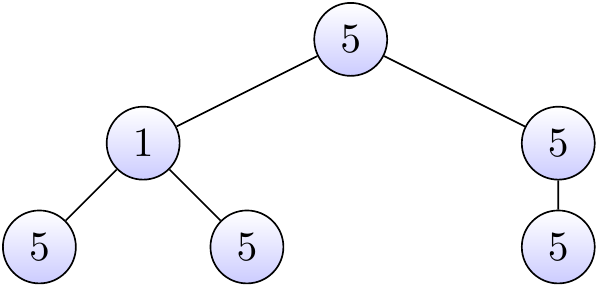
\includegraphics[width=0.9\linewidth]{tech-interview_files/figure-latex/unnamed-chunk-27-1} \caption{Some caption.}\label{fig:unnamed-chunk-27}
\end{figure}

return 4.

\hypertarget{solution-45}{%
\subsection{Solution}\label{solution-45}}

\hypertarget{walkthrough-77}{%
\subsubsection{Walkthrough\textbackslash{}}\label{walkthrough-77}}

There are \textbf{TWO} scenarios that returns true

\begin{itemize}
\tightlist
\item
  Recursively validate left node.val and right node.val == root.val
\item
  A leaf node
\end{itemize}

In addition, we need to store accumulated count across recursive function calls. Thus, data type cannot be Immutable,
since each arithmetic operation would create another object. Thus, we need to have a mutable variable that exists
across each stack frame:

\begin{itemize}
\tightlist
\item
  Have a int{[}1{]} to store the accumulated count.
\item
  Have a wrapper object to reset the value towards computation.
\item
  Have a shared variable declared for this purpose.
\end{itemize}

\hypertarget{analysis-84}{%
\subsubsection{Analysis\textbackslash{}}\label{analysis-84}}

Time complexity is O(n) as every node is visited once.

\hypertarget{algorithm-85}{%
\subsubsection{Algorithm\textbackslash{}}\label{algorithm-85}}

dfs \ref{dfs}

\hypertarget{java-code-49}{%
\subsection{Java Code}\label{java-code-49}}

\begin{Shaded}
\begin{Highlighting}[]
\DataTypeTok{int}\NormalTok{ count = }\DecValTok{0}\NormalTok{;}
\KeywordTok{public} \DataTypeTok{int} \FunctionTok{countUnivalSubtrees}\NormalTok{(}\BuiltInTok{TreeNode}\NormalTok{ root) \{}
    \FunctionTok{helper}\NormalTok{(root, count);}
    \KeywordTok{return}\NormalTok{ count;}
\NormalTok{\}}
\DataTypeTok{boolean} \FunctionTok{helper}\NormalTok{(}\BuiltInTok{TreeNode}\NormalTok{ root) \{}
    \KeywordTok{if}\NormalTok{ (root == }\KeywordTok{null}\NormalTok{) \{}
        \KeywordTok{return} \KeywordTok{true}\NormalTok{;}
\NormalTok{    \}}
    \DataTypeTok{boolean}\NormalTok{ left = }\FunctionTok{helper}\NormalTok{(root.}\FunctionTok{left}\NormalTok{);}
    \DataTypeTok{boolean}\NormalTok{ right = }\FunctionTok{helper}\NormalTok{(root.}\FunctionTok{right}\NormalTok{);}
    \KeywordTok{if}\NormalTok{ (left && right) \{}
        \CommentTok{//validate left subtree}
        \KeywordTok{if}\NormalTok{ (root.}\FunctionTok{left}\NormalTok{ != }\KeywordTok{null}\NormalTok{ && root.}\FunctionTok{left}\NormalTok{.}\FunctionTok{val}\NormalTok{ != root.}\FunctionTok{val}\NormalTok{) \{}
            \KeywordTok{return} \KeywordTok{false}\NormalTok{;}
\NormalTok{        \}}
        \CommentTok{// validate right subtree}
        \KeywordTok{if}\NormalTok{ (root.}\FunctionTok{right}\NormalTok{ != }\KeywordTok{null}\NormalTok{ && root.}\FunctionTok{right}\NormalTok{.}\FunctionTok{val}\NormalTok{ != root.}\FunctionTok{val}\NormalTok{) \{}
            \KeywordTok{return} \KeywordTok{false}\NormalTok{;}
\NormalTok{        \}}
\NormalTok{        count++;}
        \KeywordTok{return} \KeywordTok{true}\NormalTok{;}
\NormalTok{    \} }\KeywordTok{else}\NormalTok{ \{}
        \KeywordTok{return} \KeywordTok{false}\NormalTok{;}
\NormalTok{    \}}
\NormalTok{\}}
\end{Highlighting}
\end{Shaded}

\hypertarget{validate-binary-search-tree-leet-code-98-medium}{%
\section{Validate Binary Search Tree / Leet Code 98 / Medium}\label{validate-binary-search-tree-leet-code-98-medium}}

\hypertarget{description-68}{%
\subsection{Description}\label{description-68}}

Given a binary tree, determine if it is a valid binary search tree (BST). Assume a BST is defined as follows:

\begin{itemize}
\tightlist
\item
  The left subtree of a node contains only nodes with keys less than the node's key.
\item
  The right subtree of a node contains only nodes with keys greater than the node's key.
\item
  Both the left and right subtrees must also be binary search trees.
\end{itemize}

\hypertarget{example-65}{%
\subsection{Example}\label{example-65}}

\begin{figure}
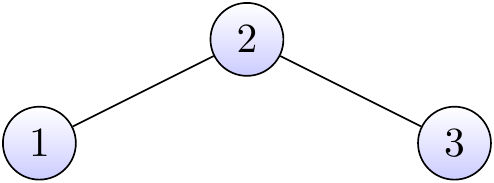
\includegraphics[width=0.9\linewidth]{tech-interview_files/figure-latex/unnamed-chunk-28-1} \caption{Some caption.}\label{fig:unnamed-chunk-28}
\end{figure}

Output: true

\begin{figure}
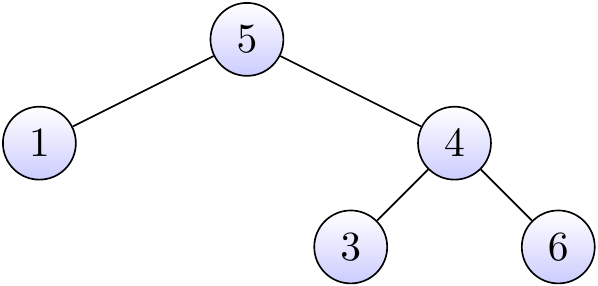
\includegraphics[width=0.9\linewidth]{tech-interview_files/figure-latex/unnamed-chunk-29-1} \caption{Some caption.}\label{fig:unnamed-chunk-29}
\end{figure}

Output: false. Explanation: The root node's value is 5 but its right child's value is 4.

\hypertarget{solution---recursive-4}{%
\subsection{Solution - Recursive}\label{solution---recursive-4}}

\hypertarget{walkthrough-78}{%
\subsubsection{Walkthrough\textbackslash{}}\label{walkthrough-78}}

For recursive, define a numeric lower and upper bounds for each validation - initially, (long) (Integer.MIN\_VALUE - 1)
and (long) (Integer.MAX\_VALUE + 1). Recursively validate the node boundary by replacing with left and right nodes.

\hypertarget{analysis-85}{%
\subsubsection{Analysis\textbackslash{}}\label{analysis-85}}

Time complexity is O(n) as every node is visited once.

\hypertarget{algorithm-86}{%
\subsubsection{Algorithm\textbackslash{}}\label{algorithm-86}}

dfs \ref{dfs}

\hypertarget{java-code---recursive-4}{%
\subsection{Java Code - Recursive}\label{java-code---recursive-4}}

\begin{Shaded}
\begin{Highlighting}[]
\KeywordTok{public} \DataTypeTok{boolean} \FunctionTok{isValidBST}\NormalTok{(}\BuiltInTok{TreeNode}\NormalTok{ root) \{}
    \KeywordTok{return} \FunctionTok{isValidBST}\NormalTok{(root, (}\DataTypeTok{long}\NormalTok{) }\BuiltInTok{Integer}\NormalTok{.}\FunctionTok{MIN_VALUE}\NormalTok{ - }\DecValTok{1}\NormalTok{, (}\DataTypeTok{long}\NormalTok{) }\BuiltInTok{Integer}\NormalTok{.}\FunctionTok{MAX_VALUE}\NormalTok{ + }\DecValTok{1}\NormalTok{);}
\NormalTok{\}}

\KeywordTok{public} \DataTypeTok{boolean} \FunctionTok{isValidBST}\NormalTok{(}\BuiltInTok{TreeNode}\NormalTok{ root, }\DataTypeTok{long}\NormalTok{ lowerBound, }\DataTypeTok{long}\NormalTok{ upperBound) \{}
    \KeywordTok{if}\NormalTok{(root == }\KeywordTok{null}\NormalTok{) \{}
        \KeywordTok{return} \KeywordTok{true}\NormalTok{;}
\NormalTok{    \} }\KeywordTok{else}\NormalTok{ \{}
        \DataTypeTok{boolean}\NormalTok{ result = root.}\FunctionTok{val}\NormalTok{ > lowerBound && root.}\FunctionTok{val}\NormalTok{ < upperBound;}
        \KeywordTok{return}\NormalTok{ result && }\FunctionTok{isValidBST}\NormalTok{(root.}\FunctionTok{left}\NormalTok{, lowerBound, root.}\FunctionTok{val}\NormalTok{) &&}
            \FunctionTok{isValidBST}\NormalTok{(root.}\FunctionTok{right}\NormalTok{, root.}\FunctionTok{val}\NormalTok{, upperBound);}
\NormalTok{    \}}
\NormalTok{\}}
\end{Highlighting}
\end{Shaded}

\hypertarget{solution---iterative-bfs-1}{%
\subsection{Solution - Iterative BFS}\label{solution---iterative-bfs-1}}

\hypertarget{walkthrough-79}{%
\subsubsection{Walkthrough\textbackslash{}}\label{walkthrough-79}}

For iterative, we have a wrapper to hold upper and lower bounds for each nodes. Use BFS to iteratively traverse the tree and
add left or right nodes with proper boundaries accordingly.

\hypertarget{analysis-86}{%
\subsubsection{Analysis\textbackslash{}}\label{analysis-86}}

Time complexity is O(n) as every node is visited once.

\hypertarget{algorithm-87}{%
\subsubsection{Algorithm\textbackslash{}}\label{algorithm-87}}

bfs \ref{bfs}

\hypertarget{java-code---iterative-bfs-1}{%
\subsection{Java Code - Iterative BFS}\label{java-code---iterative-bfs-1}}

\begin{Shaded}
\begin{Highlighting}[]
\CommentTok{//Decorator pattern}
\KeywordTok{private} \DataTypeTok{static} \KeywordTok{class}\NormalTok{ BoundedTreeNode }\KeywordTok{extends} \BuiltInTok{TreeNode}\NormalTok{ \{}
    \DataTypeTok{int}\NormalTok{ upper;}

    \DataTypeTok{int}\NormalTok{ lower;}

    \BuiltInTok{TreeNode}\NormalTok{ proxy;}

    \FunctionTok{BoundedTreeNode}\NormalTok{(}\BuiltInTok{TreeNode}\NormalTok{ node, }\DataTypeTok{int}\NormalTok{ max, }\DataTypeTok{int}\NormalTok{ min) \{}
        \KeywordTok{this}\NormalTok{.}\FunctionTok{proxy}\NormalTok{ = node;}
        \KeywordTok{this}\NormalTok{.}\FunctionTok{upper}\NormalTok{ = max;}
        \KeywordTok{this}\NormalTok{.}\FunctionTok{lower}\NormalTok{ = min;}
\NormalTok{    \}}
\NormalTok{\}}


\KeywordTok{public} \DataTypeTok{static} \DataTypeTok{boolean} \FunctionTok{validateBSTItr}\NormalTok{(}\BuiltInTok{TreeNode}\NormalTok{ root) \{}
    \KeywordTok{if}\NormalTok{(root == }\KeywordTok{null}\NormalTok{) \{}
        \KeywordTok{return} \KeywordTok{true}\NormalTok{;}
\NormalTok{    \}}

    \BuiltInTok{Queue}\NormalTok{<BoundedTreeNode> queue = }\KeywordTok{new} \BuiltInTok{LinkedList}\NormalTok{<>();}

\NormalTok{    queue.}\FunctionTok{offer}\NormalTok{(}\KeywordTok{new} \FunctionTok{BoundedTreeNode}\NormalTok{(root, }\BuiltInTok{Integer}\NormalTok{.}\FunctionTok{MAX_VALUE}\NormalTok{, }\BuiltInTok{Integer}\NormalTok{.}\FunctionTok{MIN_VALUE}\NormalTok{));}

    \KeywordTok{while}\NormalTok{(!queue.}\FunctionTok{isEmpty}\NormalTok{()) \{}
\NormalTok{        BoundedTreeNode node = queue.}\FunctionTok{poll}\NormalTok{();}


        \KeywordTok{if}\NormalTok{(node.}\FunctionTok{proxy}\NormalTok{.}\FunctionTok{data}\NormalTok{ > node.}\FunctionTok{upper}\NormalTok{ || node.}\FunctionTok{proxy}\NormalTok{.}\FunctionTok{data}\NormalTok{ < node.}\FunctionTok{lower}\NormalTok{) \{}
            \CommentTok{// out of boundary}
            \KeywordTok{return} \KeywordTok{false}\NormalTok{;}
\NormalTok{        \}}

        \KeywordTok{if}\NormalTok{(node.}\FunctionTok{proxy}\NormalTok{.}\FunctionTok{left}\NormalTok{ != }\KeywordTok{null}\NormalTok{) \{}
\NormalTok{            queue.}\FunctionTok{offer}\NormalTok{(}\KeywordTok{new} \FunctionTok{BoundedTreeNode}\NormalTok{(node.}\FunctionTok{proxy}\NormalTok{.}\FunctionTok{left}\NormalTok{, node.}\FunctionTok{proxy}\NormalTok{.}\FunctionTok{data}\NormalTok{, node.}\FunctionTok{lower}\NormalTok{));}
\NormalTok{        \}}

        \KeywordTok{if}\NormalTok{(node.}\FunctionTok{proxy}\NormalTok{.}\FunctionTok{right}\NormalTok{ != }\KeywordTok{null}\NormalTok{) \{}
\NormalTok{            queue.}\FunctionTok{offer}\NormalTok{(}\KeywordTok{new} \FunctionTok{BoundedTreeNode}\NormalTok{(node.}\FunctionTok{proxy}\NormalTok{.}\FunctionTok{right}\NormalTok{, node.}\FunctionTok{upper}\NormalTok{, node.}\FunctionTok{proxy}\NormalTok{.}\FunctionTok{data}\NormalTok{));}
\NormalTok{        \}}
\NormalTok{    \}}

    \KeywordTok{return} \KeywordTok{true}\NormalTok{;}
\NormalTok{\}}
\end{Highlighting}
\end{Shaded}

\hypertarget{binary-tree-upside-down-leet-code-156-medium}{%
\section{Binary Tree Upside Down / Leet Code 156 / Medium}\label{binary-tree-upside-down-leet-code-156-medium}}

\hypertarget{description-69}{%
\subsection{Description}\label{description-69}}

Given a binary tree where all the right nodes are either leaf nodes with a sibling (a left node that shares
the same parent node) or empty, flip it upside down and turn it into a tree where the original right nodes
turned into left leaf nodes. Return the new root.

\hypertarget{example-66}{%
\subsection{Example}\label{example-66}}

\begin{figure}
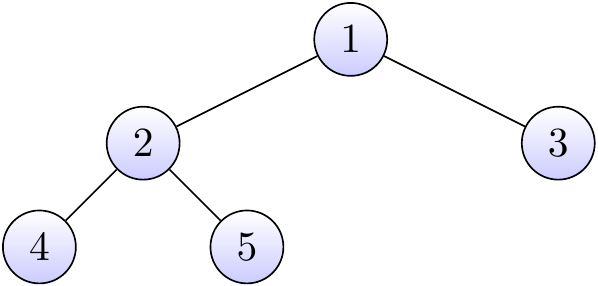
\includegraphics[width=0.9\linewidth]{tech-interview_files/figure-latex/unnamed-chunk-30-1} \caption{Some caption.}\label{fig:unnamed-chunk-30}
\end{figure}

return the root of the binary tree

\begin{figure}
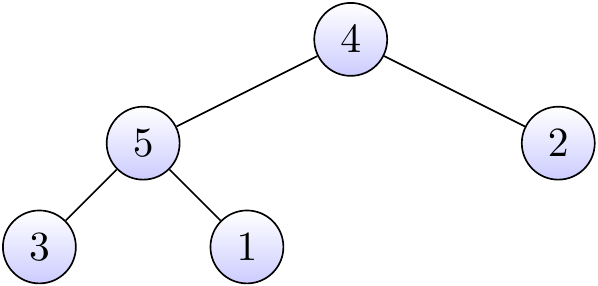
\includegraphics[width=0.9\linewidth]{tech-interview_files/figure-latex/unnamed-chunk-31-1} \caption{Some caption.}\label{fig:unnamed-chunk-31}
\end{figure}

\hypertarget{solution-46}{%
\subsection{Solution}\label{solution-46}}

\hypertarget{walkthrough-80}{%
\subsubsection{Walkthrough\textbackslash{}}\label{walkthrough-80}}

The newRoot of a flipped tree will be root.left that is

\begin{figure}
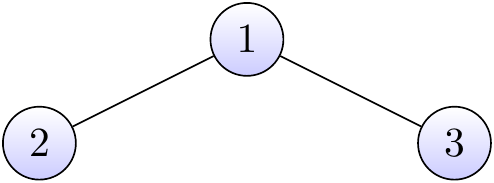
\includegraphics[width=0.9\linewidth]{tech-interview_files/figure-latex/unnamed-chunk-32-1} \caption{Some caption.}\label{fig:unnamed-chunk-32}
\end{figure}

flips to

\begin{figure}
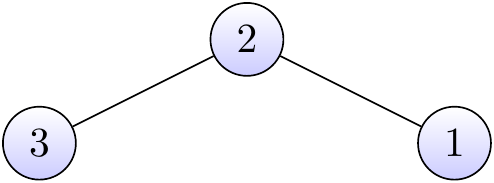
\includegraphics[width=0.9\linewidth]{tech-interview_files/figure-latex/unnamed-chunk-33-1} \caption{Some caption.}\label{fig:unnamed-chunk-33}
\end{figure}

Additionally, we need to properly place the children of root.left.

\hypertarget{analysis-87}{%
\subsubsection{Analysis\textbackslash{}}\label{analysis-87}}

Time complexity is O(n) as every node is visited once.

\hypertarget{algorithm-88}{%
\subsubsection{Algorithm\textbackslash{}}\label{algorithm-88}}

dfs \ref{dfs}

\hypertarget{java-code-50}{%
\subsection{Java Code}\label{java-code-50}}

\begin{Shaded}
\begin{Highlighting}[]
\KeywordTok{public} \BuiltInTok{TreeNode} \FunctionTok{upsideDownBinaryTree}\NormalTok{(}\BuiltInTok{TreeNode}\NormalTok{ root) \{}
    \KeywordTok{if}\NormalTok{(root == }\KeywordTok{null}\NormalTok{ || root.}\FunctionTok{left}\NormalTok{ == }\KeywordTok{null}\NormalTok{) \{}
        \KeywordTok{return}\NormalTok{ root;}
\NormalTok{    \}}

    \BuiltInTok{TreeNode}\NormalTok{ newRoot = }\FunctionTok{upsideDownBinaryTree}\NormalTok{(root.}\FunctionTok{left}\NormalTok{);}
    \CommentTok{//children of root.left}
\NormalTok{    root.}\FunctionTok{left}\NormalTok{.}\FunctionTok{left}\NormalTok{ = root.}\FunctionTok{right}\NormalTok{;}
\NormalTok{    root.}\FunctionTok{left}\NormalTok{.}\FunctionTok{right}\NormalTok{ = root;}

\NormalTok{    root.}\FunctionTok{left}\NormalTok{ = }\KeywordTok{null}\NormalTok{;}
\NormalTok{    root.}\FunctionTok{right}\NormalTok{ = }\KeywordTok{null}\NormalTok{;}
    \KeywordTok{return}\NormalTok{ newRoot;}
\NormalTok{\}}
\end{Highlighting}
\end{Shaded}

\hypertarget{inorder-successor-in-bst-leet-code-285-medium}{%
\section{Inorder Successor in BST / Leet Code 285 / Medium}\label{inorder-successor-in-bst-leet-code-285-medium}}

\hypertarget{description-70}{%
\subsection{Description}\label{description-70}}

Given a binary search tree and a node in it, find the in-order successor of that node in the BST.
Note: If the given node has no in-order successor in the tree, return null.

\hypertarget{example-67}{%
\subsection{Example}\label{example-67}}

\hypertarget{solution-47}{%
\subsection{Solution}\label{solution-47}}

\hypertarget{walkthrough-81}{%
\subsubsection{Walkthrough\textbackslash{}}\label{walkthrough-81}}

\hypertarget{analysis-88}{%
\subsubsection{Analysis\textbackslash{}}\label{analysis-88}}

Time complexity is O(n) as every node is visited once.

\hypertarget{algorithm-89}{%
\subsubsection{Algorithm\textbackslash{}}\label{algorithm-89}}

bfs \ref{bfs}

\hypertarget{java-code-51}{%
\subsection{Java Code}\label{java-code-51}}

\begin{Shaded}
\begin{Highlighting}[]
\KeywordTok{public} \BuiltInTok{TreeNode} \FunctionTok{inorderSuccessor}\NormalTok{(}\BuiltInTok{TreeNode}\NormalTok{ root, }\BuiltInTok{TreeNode}\NormalTok{ p) \{}
    \BuiltInTok{Stack}\NormalTok{<}\BuiltInTok{TreeNode}\NormalTok{> stack = }\KeywordTok{new} \BuiltInTok{Stack}\NormalTok{<}\BuiltInTok{TreeNode}\NormalTok{>();}
    \BuiltInTok{TreeNode}\NormalTok{ node = }\KeywordTok{null}\NormalTok{, prev = }\KeywordTok{null}\NormalTok{;}
    \KeywordTok{while}\NormalTok{ (!stack.}\FunctionTok{isEmpty}\NormalTok{() || node != }\KeywordTok{null}\NormalTok{) \{}
        \KeywordTok{if}\NormalTok{ (node != }\KeywordTok{null}\NormalTok{) \{}
\NormalTok{            stack.}\FunctionTok{push}\NormalTok{(node);}
\NormalTok{            node = node.}\FunctionTok{left}\NormalTok{;}
\NormalTok{        \} }\KeywordTok{else}\NormalTok{ \{}
\NormalTok{            node = stack.}\FunctionTok{pop}\NormalTok{();}
            \KeywordTok{if}\NormalTok{ (prev == p) \{}
                \KeywordTok{return}\NormalTok{ node;}
\NormalTok{            \}}
\NormalTok{            prev = node;}
\NormalTok{            node = node.}\FunctionTok{right}\NormalTok{;}
\NormalTok{        \}}
\NormalTok{    \}}
    \KeywordTok{return} \KeywordTok{null}\NormalTok{;}
\NormalTok{\}}
\end{Highlighting}
\end{Shaded}

\hypertarget{binary-tree-longest-consecutive-sequence-leet-code-298-medium}{%
\section{Binary Tree Longest Consecutive Sequence / Leet Code 298 / Medium}\label{binary-tree-longest-consecutive-sequence-leet-code-298-medium}}

\hypertarget{description-71}{%
\subsection{Description}\label{description-71}}

Given a binary tree, find the length of the longest consecutive sequence path.
The path refers to any sequence of nodes from some starting node to any node in the tree along the parent-child
connections. The longest consecutive path need to be from parent to child (cannot be the reverse).

\hypertarget{example-68}{%
\subsection{Example}\label{example-68}}

\begin{figure}
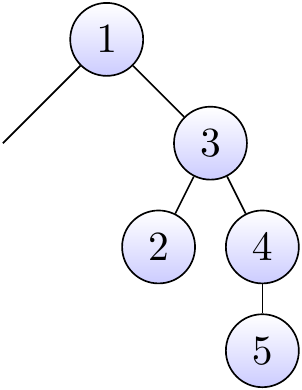
\includegraphics[width=0.9\linewidth]{tech-interview_files/figure-latex/unnamed-chunk-34-1} \caption{Some caption.}\label{fig:unnamed-chunk-34}
\end{figure}

Longest consecutive sequence path is 3-4-5, so return 3.

\begin{figure}
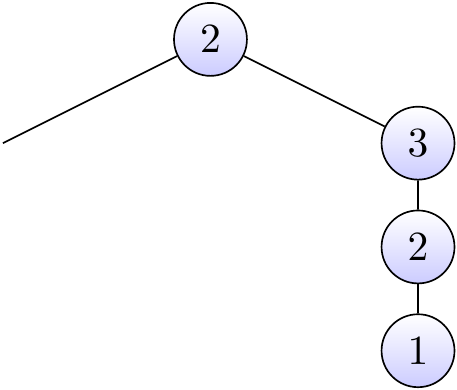
\includegraphics[width=0.9\linewidth]{tech-interview_files/figure-latex/unnamed-chunk-35-1} \caption{Some caption.}\label{fig:unnamed-chunk-35}
\end{figure}

Longest consecutive sequence path is 2-3,not3-2-1, so return 2.

\hypertarget{solution-48}{%
\subsection{Solution}\label{solution-48}}

\hypertarget{walkthrough-82}{%
\subsubsection{Walkthrough\textbackslash{}}\label{walkthrough-82}}

For each recursive call,

\begin{itemize}
\tightlist
\item
  if root.val == target, length++
\item
  otherwise, reset length = 1
\end{itemize}

Retrieve for the maximum length and recursively call on left and right subtrees with increasing sequence
(root.val + 1).

If we want longest increaing sequence, change to (root.val \textgreater{}= target) to verify increasing sequence.

\hypertarget{analysis-89}{%
\subsubsection{Analysis\textbackslash{}}\label{analysis-89}}

Time complexity is O(n) as every node is visited once.

\hypertarget{algorithm-90}{%
\subsubsection{Algorithm\textbackslash{}}\label{algorithm-90}}

dfs \ref{dfs}

\hypertarget{java-code-52}{%
\subsection{Java Code}\label{java-code-52}}

\begin{Shaded}
\begin{Highlighting}[]
\KeywordTok{private} \DataTypeTok{int}\NormalTok{ longest;}

\KeywordTok{public} \DataTypeTok{int} \FunctionTok{longestConsecutive}\NormalTok{(}\BuiltInTok{TreeNode}\NormalTok{ root) \{}
    \KeywordTok{if}\NormalTok{ (root == }\KeywordTok{null}\NormalTok{) \{}
        \KeywordTok{return} \DecValTok{0}\NormalTok{;}
\NormalTok{    \}}

    \FunctionTok{longestConsecutive}\NormalTok{(root, }\DecValTok{0}\NormalTok{, root.}\FunctionTok{val}\NormalTok{);}

    \KeywordTok{return}\NormalTok{ longest;}
\NormalTok{\}}
\KeywordTok{public} \DataTypeTok{void} \FunctionTok{longestConsecutive}\NormalTok{(}\BuiltInTok{TreeNode}\NormalTok{ root, }\DataTypeTok{int}\NormalTok{ length, }\DataTypeTok{int}\NormalTok{ target) \{}
    \KeywordTok{if}\NormalTok{ (root == }\KeywordTok{null}\NormalTok{) \{}
        \KeywordTok{return}\NormalTok{;}
\NormalTok{    \} }\KeywordTok{else} \KeywordTok{if}\NormalTok{ (root.}\FunctionTok{val}\NormalTok{ == target) \{}
\NormalTok{        length++;}
\NormalTok{    \} }\KeywordTok{else}\NormalTok{ \{}
\NormalTok{        length = }\DecValTok{1}\NormalTok{;}
\NormalTok{    \}}

\NormalTok{    longest = }\BuiltInTok{Math}\NormalTok{.}\FunctionTok{max}\NormalTok{(longest, length);}

    \CommentTok{//root.val + 1 for increasing sequencef}
    \FunctionTok{longestConsecutive}\NormalTok{(root.}\FunctionTok{left}\NormalTok{, length, root.}\FunctionTok{val}\NormalTok{ + }\DecValTok{1}\NormalTok{);}
    \FunctionTok{longestConsecutive}\NormalTok{(root.}\FunctionTok{right}\NormalTok{, length, root.}\FunctionTok{val}\NormalTok{ + }\DecValTok{1}\NormalTok{);}
\NormalTok{\}}
\end{Highlighting}
\end{Shaded}

\hypertarget{find-leaves-of-binary-tree-leet-code-366-medium}{%
\section{Find Leaves of Binary Tree / Leet Code 366 / Medium}\label{find-leaves-of-binary-tree-leet-code-366-medium}}

\hypertarget{description-72}{%
\subsection{Description}\label{description-72}}

Given a binary tree, collect a tree's nodes as if you were doing this: Collect and remove all leaves, repeat
until the tree is empty.

\hypertarget{example-69}{%
\subsection{Example}\label{example-69}}

\begin{figure}
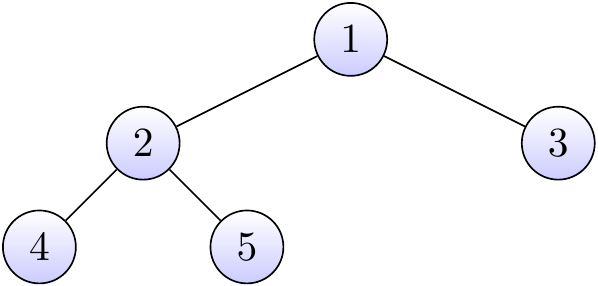
\includegraphics[width=0.9\linewidth]{tech-interview_files/figure-latex/unnamed-chunk-36-1} \caption{Some caption.}\label{fig:unnamed-chunk-36}
\end{figure}

Returns {[}4, 5, 3{]}, {[}2{]}, {[}1{]}.

\hypertarget{solution-49}{%
\subsection{Solution}\label{solution-49}}

\hypertarget{walkthrough-83}{%
\subsubsection{Walkthrough\textbackslash{}}\label{walkthrough-83}}

For each node, compute maximum level (leaf node is -1) out of recursive call to left and right subtree + 1.
If level increases, add a new list and add the node.val into the list -- list.add(node.val)

\hypertarget{analysis-90}{%
\subsubsection{Analysis\textbackslash{}}\label{analysis-90}}

Time complexity is O(n) as every node is visited once.

\hypertarget{algorithm-91}{%
\subsubsection{Algorithm\textbackslash{}}\label{algorithm-91}}

dfs \ref{dfs}

\hypertarget{java-code-53}{%
\subsection{Java Code}\label{java-code-53}}

\begin{Shaded}
\begin{Highlighting}[]
\KeywordTok{public} \BuiltInTok{List}\NormalTok{<}\BuiltInTok{List}\NormalTok{<}\BuiltInTok{Integer}\NormalTok{>> }\FunctionTok{findLeaves}\NormalTok{(}\BuiltInTok{TreeNode}\NormalTok{ root) \{}
    \BuiltInTok{List}\NormalTok{<}\BuiltInTok{List}\NormalTok{<}\BuiltInTok{Integer}\NormalTok{>> result = }\KeywordTok{new} \BuiltInTok{LinkedList}\NormalTok{<}\BuiltInTok{List}\NormalTok{<}\BuiltInTok{Integer}\NormalTok{>>();}
    \FunctionTok{helper}\NormalTok{(root, result);}

    \KeywordTok{return}\NormalTok{ result;}
\NormalTok{\}}
\KeywordTok{private} \DataTypeTok{int} \FunctionTok{helper}\NormalTok{(}\BuiltInTok{TreeNode}\NormalTok{ root, }\BuiltInTok{List}\NormalTok{<}\BuiltInTok{List}\NormalTok{<}\BuiltInTok{Integer}\NormalTok{>> result) \{}
    \KeywordTok{if}\NormalTok{ (root == }\KeywordTok{null}\NormalTok{) \{}
        \KeywordTok{return} \DecValTok{-1}\NormalTok{;}
\NormalTok{    \}}

    \DataTypeTok{int}\NormalTok{ level = }\BuiltInTok{Math}\NormalTok{.}\FunctionTok{max}\NormalTok{(}\FunctionTok{helper}\NormalTok{(root.}\FunctionTok{left}\NormalTok{, result), }\FunctionTok{helper}\NormalTok{(root.}\FunctionTok{right}\NormalTok{, result)) + }\DecValTok{1}\NormalTok{;}

    \CommentTok{//add a new level if level increases}
    \KeywordTok{if}\NormalTok{ (result.}\FunctionTok{size}\NormalTok{() <= level) \{}
\NormalTok{        result.}\FunctionTok{add}\NormalTok{(}\KeywordTok{new} \BuiltInTok{LinkedList}\NormalTok{<}\BuiltInTok{Integer}\NormalTok{>());}
\NormalTok{    \}}

    \CommentTok{//add root.val}
\NormalTok{    result.}\FunctionTok{get}\NormalTok{(level).}\FunctionTok{add}\NormalTok{(root.}\FunctionTok{val}\NormalTok{);}

    \KeywordTok{return}\NormalTok{ level;}
\NormalTok{\}}
\end{Highlighting}
\end{Shaded}

\hypertarget{diameter-of-binary-tree-leet-code-543-easy}{%
\section{Diameter of Binary Tree / Leet Code 543 / Easy}\label{diameter-of-binary-tree-leet-code-543-easy}}

\hypertarget{description-73}{%
\subsection{Description}\label{description-73}}

Given a binary tree, you need to compute the length of the diameter of the tree. The diameter of a binary tree is the
length of the longest path between any two nodes in a tree. This path may or may not pass through the root.

\hypertarget{example-70}{%
\subsection{Example}\label{example-70}}

Given a binary tree

\begin{figure}
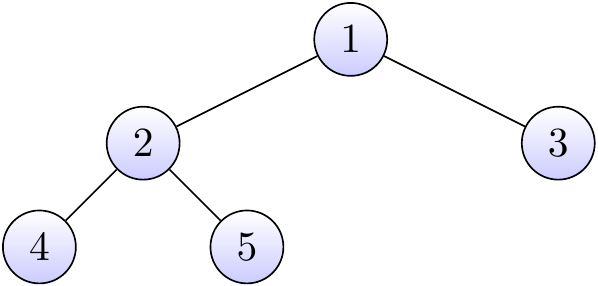
\includegraphics[width=0.9\linewidth]{tech-interview_files/figure-latex/unnamed-chunk-37-1} \caption{Some caption.}\label{fig:unnamed-chunk-37}
\end{figure}

Return 3, which is the length of the path {[}4,2,1,3{]} or {[}5,2,1,3{]}.
Note: The length of path between two nodes is represented by the number of edges between them.

\hypertarget{solution-50}{%
\subsection{Solution}\label{solution-50}}

\hypertarget{walkthrough-84}{%
\subsubsection{Walkthrough\textbackslash{}}\label{walkthrough-84}}

Have a help function to compute the left and right height as well as diameter (left height + right height). Find the
maximum diameter among root, left and right.

\hypertarget{analysis-91}{%
\subsubsection{Analysis\textbackslash{}}\label{analysis-91}}

Time complexity is O(n) as every node is visited once.

\hypertarget{algorithm-92}{%
\subsubsection{Algorithm\textbackslash{}}\label{algorithm-92}}

dfs \ref{dfs}

\hypertarget{java-code-54}{%
\subsection{Java Code}\label{java-code-54}}

\begin{Shaded}
\begin{Highlighting}[]
\KeywordTok{public} \DataTypeTok{int} \FunctionTok{diameterOfBinaryTree}\NormalTok{(}\BuiltInTok{TreeNode}\NormalTok{ root) \{}
    \DataTypeTok{int}\NormalTok{[] result = }\FunctionTok{diameterAndHeight}\NormalTok{(root);}
    \KeywordTok{return}\NormalTok{ result[}\DecValTok{0}\NormalTok{];}
\NormalTok{\}}

\KeywordTok{public} \DataTypeTok{int}\NormalTok{[] }\FunctionTok{diameterAndHeight}\NormalTok{(}\BuiltInTok{TreeNode}\NormalTok{ root) \{}
    \DataTypeTok{int}\NormalTok{ heightDiameter[] = \{ }\DecValTok{0}\NormalTok{, }\DecValTok{0}\NormalTok{ \};          }\CommentTok{// initialize the diameter and height}

    \KeywordTok{if}\NormalTok{ (root != }\KeywordTok{null}\NormalTok{) \{}
        \DataTypeTok{int}\NormalTok{[] leftResult = }\FunctionTok{diameterAndHeight}\NormalTok{(root.}\FunctionTok{left}\NormalTok{);}
        \DataTypeTok{int}\NormalTok{[] rightResult = }\FunctionTok{diameterAndHeight}\NormalTok{(root.}\FunctionTok{right}\NormalTok{);}
        \DataTypeTok{int}\NormalTok{ height = }\BuiltInTok{Math}\NormalTok{.}\FunctionTok{max}\NormalTok{(leftResult[}\DecValTok{1}\NormalTok{], rightResult[}\DecValTok{1}\NormalTok{]) + }\DecValTok{1}\NormalTok{;}
        \DataTypeTok{int}\NormalTok{ leftDiameter = leftResult[}\DecValTok{0}\NormalTok{];}
        \DataTypeTok{int}\NormalTok{ rightDiameter = rightResult[}\DecValTok{0}\NormalTok{];}
        \DataTypeTok{int}\NormalTok{ rootDiameter = leftResult[}\DecValTok{1}\NormalTok{] + rightResult[}\DecValTok{1}\NormalTok{];}
        \DataTypeTok{int}\NormalTok{ finalDiameter = }\BuiltInTok{Math}\NormalTok{.}\FunctionTok{max}\NormalTok{(rootDiameter, }\BuiltInTok{Math}\NormalTok{.}\FunctionTok{max}\NormalTok{(leftDiameter, rightDiameter));}
\NormalTok{        heightDiameter[}\DecValTok{0}\NormalTok{] = finalDiameter;}
\NormalTok{        heightDiameter[}\DecValTok{1}\NormalTok{] = height;}
\NormalTok{    \}}
    \KeywordTok{return}\NormalTok{ heightDiameter;}
\NormalTok{\}}
\end{Highlighting}
\end{Shaded}

\hypertarget{binary-tree-serialization-firecode-level-3}{%
\section{Binary Tree Serialization / Firecode / Level 3}\label{binary-tree-serialization-firecode-level-3}}

\hypertarget{description-74}{%
\subsection{Description}\label{description-74}}

In Computer Science, serialization is the process of converting objects or data structures into a sequence (or series)
of characters that can be stored easily in a file / database table or transmitted across a network. Serialized objects
need to be de-serialized to create a semantically identical clone of the original object, before being used in programs.
You're given the root node of a binary tree - TreeNode root in the method serializeTree. This method should serialize
the binary tree and output a String str, which is then used as an input parameter for the method restoreTree.
restoreTree should create a Binary Tree that is structurally identical to the one you serialized and return the root
node of the tree. Your task is to fill in the logic for these 2 methods. Don't worry about passing the serialized String
to restoreTree - that will be done automatically when you run your code. Feel free to use any notation you prefer when
serializing the binary tree. The choice of traversal algorithm is also open - but try and limit the time complexity of
both methods to O(n).

\hypertarget{example-71}{%
\subsection{Example}\label{example-71}}

\hypertarget{solution-51}{%
\subsection{Solution}\label{solution-51}}

\hypertarget{walkthrough-85}{%
\subsubsection{Walkthrough\textbackslash{}}\label{walkthrough-85}}

Your serialized String will be used to restore the tree. Be sure to use the same format and notation in restoreTree
that you use to serialize in serializeTree. For example, the following binary tree

\begin{figure}
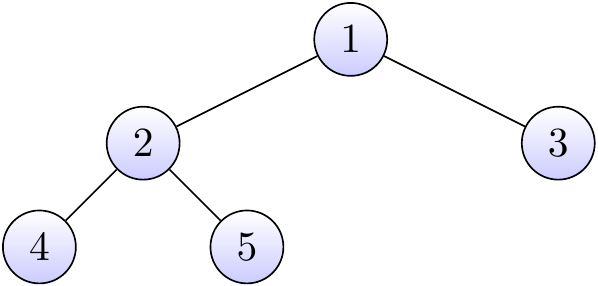
\includegraphics[width=0.9\linewidth]{tech-interview_files/figure-latex/unnamed-chunk-38-1} \caption{Some caption.}\label{fig:unnamed-chunk-38}
\end{figure}

would be serialize into string ``1 2 4 \# \# 5 \# \# 3 \# \#''.

\hypertarget{analysis-92}{%
\subsubsection{Analysis\textbackslash{}}\label{analysis-92}}

Time complexity is O(n) as every node is visited once.

\hypertarget{algorithm-93}{%
\subsubsection{Algorithm\textbackslash{}}\label{algorithm-93}}

dfs \ref{dfs}

\hypertarget{java-code-55}{%
\subsection{Java Code}\label{java-code-55}}

\begin{Shaded}
\begin{Highlighting}[]
\KeywordTok{public} \BuiltInTok{String} \FunctionTok{serializeTree}\NormalTok{(}\BuiltInTok{TreeNode}\NormalTok{ root)\{}
    \BuiltInTok{StringBuilder}\NormalTok{ sb = }\KeywordTok{new} \BuiltInTok{StringBuilder}\NormalTok{();}

    \KeywordTok{if}\NormalTok{ (root == }\KeywordTok{null}\NormalTok{) \{}
\NormalTok{        sb.}\FunctionTok{append}\NormalTok{(}\StringTok{"# "}\NormalTok{);}
\NormalTok{    \} }\KeywordTok{else}\NormalTok{ \{}
\NormalTok{        sb.}\FunctionTok{append}\NormalTok{(root.}\FunctionTok{data}\NormalTok{ + }\StringTok{" "}\NormalTok{);}
\NormalTok{        sb.}\FunctionTok{append}\NormalTok{(}\FunctionTok{serializeTree}\NormalTok{(root.}\FunctionTok{left}\NormalTok{));}
\NormalTok{        sb.}\FunctionTok{append}\NormalTok{(}\FunctionTok{serializeTree}\NormalTok{(root.}\FunctionTok{right}\NormalTok{));}
\NormalTok{    \}}

    \KeywordTok{return}\NormalTok{ sb.}\FunctionTok{toString}\NormalTok{();}
\NormalTok{\}}

\KeywordTok{public} \BuiltInTok{TreeNode} \FunctionTok{restoreTree}\NormalTok{(}\BuiltInTok{String}\NormalTok{ str)\{}
    \KeywordTok{if}\NormalTok{ (str == }\KeywordTok{null}\NormalTok{ || str.}\FunctionTok{length}\NormalTok{() == }\DecValTok{0}\NormalTok{) \{}
        \KeywordTok{return} \KeywordTok{null}\NormalTok{;}
\NormalTok{    \}}

    \BuiltInTok{StringTokenizer}\NormalTok{ tokenizer = }\KeywordTok{new} \BuiltInTok{StringTokenizer}\NormalTok{(str, }\StringTok{" "}\NormalTok{);}
    \KeywordTok{return} \FunctionTok{deserialize}\NormalTok{(tokenizer);}
\NormalTok{\}}

\KeywordTok{private} \BuiltInTok{TreeNode} \FunctionTok{deserialize}\NormalTok{(}\BuiltInTok{StringTokenizer}\NormalTok{ tokenizer)\{}
    \KeywordTok{if}\NormalTok{ (!tokenizer.}\FunctionTok{hasMoreTokens}\NormalTok{()) \{}
        \KeywordTok{return} \KeywordTok{null}\NormalTok{;}
\NormalTok{    \}}
    \BuiltInTok{String}\NormalTok{ val = tokenizer.}\FunctionTok{nextToken}\NormalTok{();}

    \KeywordTok{if}\NormalTok{ (val.}\FunctionTok{equals}\NormalTok{(}\StringTok{"#"}\NormalTok{)) \{}
        \KeywordTok{return} \KeywordTok{null}\NormalTok{;}
\NormalTok{    \}}

    \BuiltInTok{TreeNode}\NormalTok{ root = }\KeywordTok{new} \BuiltInTok{TreeNode}\NormalTok{(}\BuiltInTok{Integer}\NormalTok{.}\FunctionTok{parseInt}\NormalTok{(val));}
\NormalTok{    root.}\FunctionTok{left}\NormalTok{ = }\FunctionTok{deserialize}\NormalTok{(tokenizer);}
\NormalTok{    root.}\FunctionTok{right}\NormalTok{ = }\FunctionTok{deserialize}\NormalTok{(tokenizer);}

    \KeywordTok{return}\NormalTok{ root;}
\NormalTok{\}}
\end{Highlighting}
\end{Shaded}

\hypertarget{fill-in-the-ancestors-of-the-node-in-a-binary-tree-firebase-level-3}{%
\section{Fill in the Ancestors of the Node in a Binary Tree / Firebase / Level 3}\label{fill-in-the-ancestors-of-the-node-in-a-binary-tree-firebase-level-3}}

\hypertarget{description-75}{%
\subsection{Description}\label{description-75}}

Given a binary tree's root node, an empty ArrayList and an integer nodeData, write a method that finds a target
node - N with data = nodeData and populates the ArrayList with the data of the ancestor nodes of N - added from the
bottom - up

\hypertarget{algorithm-94}{%
\subsubsection{Algorithm\textbackslash{}}\label{algorithm-94}}

dfs \ref{dfs}, backtrack \ref{backtrack}

\hypertarget{example-72}{%
\subsection{Example}\label{example-72}}

\begin{figure}
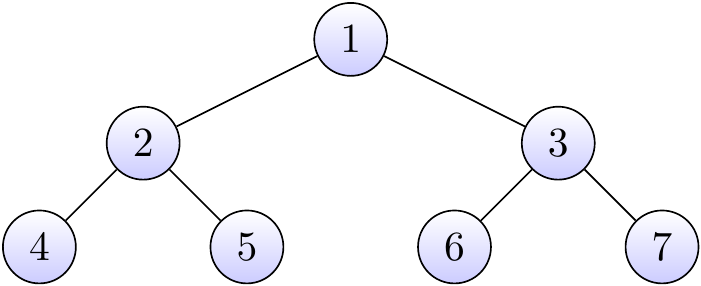
\includegraphics[width=0.9\linewidth]{tech-interview_files/figure-latex/unnamed-chunk-39-1} \caption{Some caption.}\label{fig:unnamed-chunk-39}
\end{figure}

Node: 5 = {[}2, 1{]}

\hypertarget{solution-52}{%
\subsection{Solution}\label{solution-52}}

\hypertarget{walkthrough-86}{%
\subsubsection{Walkthrough\textbackslash{}}\label{walkthrough-86}}

We use an arrayList to keep the current path of TreeNode visited, also TreeNode to be removed for backtracking purposes.
We use recurisve call and terminate on leave nodes as well as target node is found. The recursive function returns a
boolean value when the target node / value is found on the subtree path.

\hypertarget{analysis-93}{%
\subsubsection{Analysis\textbackslash{}}\label{analysis-93}}

Time complexity is O(n) as every node is visited once.

\hypertarget{algorithm-95}{%
\subsubsection{Algorithm\textbackslash{}}\label{algorithm-95}}

dfs \ref{dfs}, backtrack \ref{backtrack}

\hypertarget{java-code-56}{%
\subsection{Java Code}\label{java-code-56}}

\begin{Shaded}
\begin{Highlighting}[]
\KeywordTok{public} \BuiltInTok{ArrayList}\NormalTok{<}\BuiltInTok{Integer}\NormalTok{> ancestorsList = }\KeywordTok{new} \BuiltInTok{ArrayList}\NormalTok{<}\BuiltInTok{Integer}\NormalTok{>();}

\KeywordTok{public} \DataTypeTok{boolean} \FunctionTok{printAncestors}\NormalTok{(}\BuiltInTok{TreeNode}\NormalTok{ root, }\DataTypeTok{int}\NormalTok{ nodeData) \{}
    \KeywordTok{if}\NormalTok{(root == }\KeywordTok{null}\NormalTok{) \{}
        \KeywordTok{return} \KeywordTok{false}\NormalTok{;}
\NormalTok{    \}}

    \KeywordTok{if}\NormalTok{(root.}\FunctionTok{data}\NormalTok{ == nodeData) \{}
        \KeywordTok{return} \KeywordTok{true}\NormalTok{;}
\NormalTok{    \} }\KeywordTok{else}\NormalTok{ \{}
\NormalTok{        ancestorsList.}\FunctionTok{add}\NormalTok{(}\DecValTok{0}\NormalTok{, root.}\FunctionTok{data}\NormalTok{);}

        \DataTypeTok{boolean}\NormalTok{ isRightSubtree = }\FunctionTok{printAncestors}\NormalTok{(root.}\FunctionTok{left}\NormalTok{, nodeData) || }\FunctionTok{printAncestors}\NormalTok{(root.}\FunctionTok{right}\NormalTok{, nodeData);}

        \KeywordTok{if}\NormalTok{(!isRightSubtree) \{}
            \CommentTok{//remove the backtrack nodes}
\NormalTok{            ancestorsList.}\FunctionTok{remove}\NormalTok{(}\DecValTok{0}\NormalTok{);}
\NormalTok{        \}}

        \KeywordTok{return}\NormalTok{ isRightSubtree;}
\NormalTok{    \}}
\NormalTok{\}}
\end{Highlighting}
\end{Shaded}

\section{Find the $k^{th}$ Largest Node in a BST / Firecode / Level 3}

\hypertarget{description-76}{%
\subsection{Description}\label{description-76}}

Given a Binary Search Tree and an integer k, implement a method to find and return its \(k^{th}\) largest node

\hypertarget{example-73}{%
\subsection{Example}\label{example-73}}

\begin{figure}
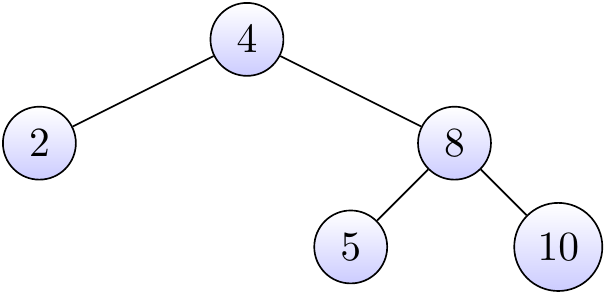
\includegraphics[width=0.9\linewidth]{tech-interview_files/figure-latex/unnamed-chunk-40-1} \caption{Some caption.}\label{fig:unnamed-chunk-40}
\end{figure}

In the above scenario, if k = 1, then the output is 10 i.e.~k = 1, represents the largest element of the tree,
k = 2, represents the second largest element and so on.

\hypertarget{solution-53}{%
\subsection{Solution}\label{solution-53}}

\hypertarget{walkthrough-87}{%
\subsubsection{Walkthrough\textbackslash{}}\label{walkthrough-87}}

First we compute the size of right subtree, and evaluate the following possibilities

\begin{itemize}
\tightlist
\item
  if k == (sizeOfRightSubtree + 1), return this node
\item
  if k \(<\) sizeOfRightSubtree, the target must reside in the right subtree. Drill down to right subtree
\item
  if k \(>\) sizeOfRightSubtree, the target must reside in the left subtree. Drill down to the left subtree and
  change target position to (k - sizeOfRightSubtree - 1)
\end{itemize}

\hypertarget{analysis-94}{%
\subsubsection{Analysis\textbackslash{}}\label{analysis-94}}

Time complexity is O(log(n)) as a certain path of nodes will be visited since this is a BST.

\hypertarget{algorithm-96}{%
\subsubsection{Algorithm\textbackslash{}}\label{algorithm-96}}

dfs \ref{dfs}, bst \ref{bst}

\hypertarget{java-code-57}{%
\subsection{Java Code}\label{java-code-57}}

\begin{Shaded}
\begin{Highlighting}[]
\KeywordTok{public} \BuiltInTok{TreeNode} \FunctionTok{findKthLargest}\NormalTok{(}\BuiltInTok{TreeNode}\NormalTok{ root, }\DataTypeTok{int}\NormalTok{ k) \{}
    \KeywordTok{if}\NormalTok{(root == }\KeywordTok{null}\NormalTok{) \{}
        \KeywordTok{return} \KeywordTok{null}\NormalTok{;}
\NormalTok{    \}}

    \DataTypeTok{int}\NormalTok{ rightSubtreeSize = }\FunctionTok{size}\NormalTok{(root.}\FunctionTok{right}\NormalTok{);}

    \KeywordTok{if}\NormalTok{( (rightSubtreeSize + }\DecValTok{1}\NormalTok{) == k) \{}
        \KeywordTok{return}\NormalTok{ root;}
\NormalTok{    \} }\KeywordTok{else} \KeywordTok{if}\NormalTok{( rightSubtreeSize > k ) \{}
        \CommentTok{//drill down to the right subtree}
        \KeywordTok{return} \FunctionTok{findKthLargest}\NormalTok{(root.}\FunctionTok{right}\NormalTok{, k);}
\NormalTok{    \} }\KeywordTok{else}\NormalTok{ \{}
        \CommentTok{//drill down to the left subtree}
        \KeywordTok{return} \FunctionTok{findKthLargest}\NormalTok{(root.}\FunctionTok{left}\NormalTok{, k - rightSubtreeSize - }\DecValTok{1}\NormalTok{);}
\NormalTok{    \}}
\NormalTok{\}}
\end{Highlighting}
\end{Shaded}

\hypertarget{convert-sorted-array-to-binary-search-tree-leet-code-108-easy}{%
\section{Convert Sorted Array to Binary Search Tree / Leet Code 108 / Easy}\label{convert-sorted-array-to-binary-search-tree-leet-code-108-easy}}

\hypertarget{description-77}{%
\subsection{Description}\label{description-77}}

Given an array where elements are sorted in ascending order, convert it to a height balanced BST.

For this problem, a height-balanced binary tree is defined as a binary tree in which the depth of the two subtrees of
every node never differ by more than 1

\hypertarget{example-74}{%
\subsection{Example}\label{example-74}}

\begin{figure}
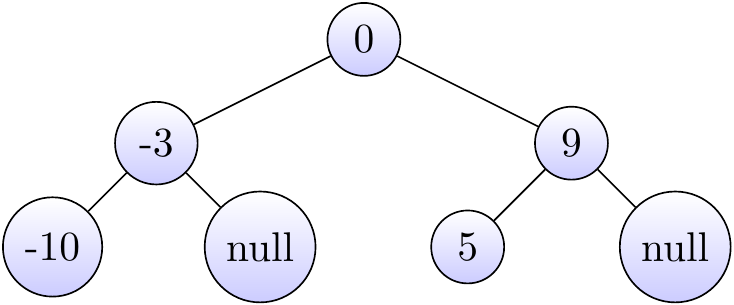
\includegraphics[width=0.9\linewidth]{tech-interview_files/figure-latex/unnamed-chunk-41-1} \caption{Some caption.}\label{fig:unnamed-chunk-41}
\end{figure}

\hypertarget{solution-54}{%
\subsection{Solution}\label{solution-54}}

\hypertarget{walkthrough-88}{%
\subsubsection{Walkthrough\textbackslash{}}\label{walkthrough-88}}

To create a tree of minimal height, we need to mathch the number of nodes in the left subtree to the number of the
nodes in the right subtree as much as possible. This means that we want the root to be the middle of the \textbf{sorted }
array, since this would mean that half the elements would be less than the root and half wood be greater than it.

\hypertarget{analysis-95}{%
\subsubsection{Analysis\textbackslash{}}\label{analysis-95}}

The overal time complexity is O(n) as every node is visited once.

\hypertarget{algorithm-97}{%
\subsubsection{Algorithm\textbackslash{}}\label{algorithm-97}}

dfs \ref{dfs}

\hypertarget{java-code-58}{%
\subsection{Java Code}\label{java-code-58}}

\begin{Shaded}
\begin{Highlighting}[]
\KeywordTok{public} \BuiltInTok{TreeNode} \FunctionTok{sortedArrayToBST}\NormalTok{(}\DataTypeTok{int}\NormalTok{[] nums) \{}
    \KeywordTok{return} \FunctionTok{buildHeightBalancedBST}\NormalTok{(nums, }\DecValTok{0}\NormalTok{, nums.}\FunctionTok{length} \DecValTok{-1}\NormalTok{);}
\NormalTok{\}}

\KeywordTok{public} \BuiltInTok{TreeNode} \FunctionTok{buildHeightBalancedBST}\NormalTok{(}\DataTypeTok{int}\NormalTok{[] nums, }\DataTypeTok{int}\NormalTok{ start, }\DataTypeTok{int}\NormalTok{ end) \{}
    \KeywordTok{if}\NormalTok{(start > end) \{}
        \KeywordTok{return} \KeywordTok{null}\NormalTok{;}
\NormalTok{    \}}

    \DataTypeTok{int}\NormalTok{ mid = (start + end) / }\DecValTok{2}\NormalTok{;}
    \BuiltInTok{TreeNode}\NormalTok{ node = }\KeywordTok{new} \BuiltInTok{TreeNode}\NormalTok{(nums[mid]);}
\NormalTok{    node.}\FunctionTok{left}\NormalTok{ = }\FunctionTok{buildHeightBalancedBST}\NormalTok{(nums, start, mid - }\DecValTok{1}\NormalTok{);}
\NormalTok{    node.}\FunctionTok{right}\NormalTok{ = }\FunctionTok{buildHeightBalancedBST}\NormalTok{(nums, mid + }\DecValTok{1}\NormalTok{, end);}

    \KeywordTok{return}\NormalTok{ node;}
\NormalTok{\}}
\end{Highlighting}
\end{Shaded}

\hypertarget{populating-next-right-pointers-in-each-node-leet-code-116-medium}{%
\section{Populating Next Right Pointers in Each Node / Leet Code 116 / Medium}\label{populating-next-right-pointers-in-each-node-leet-code-116-medium}}

\hypertarget{description-78}{%
\subsection{Description}\label{description-78}}

You are given a perfect binary tree where all leaves are on the same level, and every parent has two children.
Populate each next pointer to point to its next right node. If there is no next right node, the next pointer should
be set to NULL. Initially, all next pointers are set to NULL.

\hypertarget{example-75}{%
\subsection{Example}\label{example-75}}

\hypertarget{solution-55}{%
\subsection{Solution}\label{solution-55}}

\hypertarget{walkthrough-89}{%
\subsubsection{Walkthrough\textbackslash{}}\label{walkthrough-89}}

\hypertarget{analysis-96}{%
\subsubsection{Analysis\textbackslash{}}\label{analysis-96}}

Time complexity is O(n) as every node is visited once.

\hypertarget{algorithm-98}{%
\subsubsection{Algorithm\textbackslash{}}\label{algorithm-98}}

dfs \ref{dfs}

\hypertarget{java-code---preorder-recursive}{%
\subsection{Java Code - PreOrder Recursive}\label{java-code---preorder-recursive}}

\begin{Shaded}
\begin{Highlighting}[]
\KeywordTok{public} \BuiltInTok{Node} \FunctionTok{connect}\NormalTok{(}\BuiltInTok{Node}\NormalTok{ root) \{}
    \KeywordTok{if}\NormalTok{(root == }\KeywordTok{null}\NormalTok{)\{}
        \KeywordTok{return}\NormalTok{ root;}
\NormalTok{    \}}

    \KeywordTok{if}\NormalTok{(root.}\FunctionTok{left}\NormalTok{ == }\KeywordTok{null}\NormalTok{) \{}
        \KeywordTok{return}\NormalTok{ root;}
\NormalTok{    \}}

    \CommentTok{// populate left child.next => right child}
\NormalTok{    root.}\FunctionTok{left}\NormalTok{.}\FunctionTok{next}\NormalTok{=root.}\FunctionTok{right}\NormalTok{;}

    \CommentTok{// previously populated, i.e. root(2)}
    \KeywordTok{if}\NormalTok{(root.}\FunctionTok{next}\NormalTok{ != }\KeywordTok{null}\NormalTok{)\{}
        \CommentTok{//root.next = 3 which connects to another branch}
\NormalTok{        root.}\FunctionTok{right}\NormalTok{.}\FunctionTok{next}\NormalTok{=root.}\FunctionTok{next}\NormalTok{.}\FunctionTok{left}\NormalTok{;}
\NormalTok{    \}}

    \FunctionTok{connect}\NormalTok{(root.}\FunctionTok{left}\NormalTok{);}
    \FunctionTok{connect}\NormalTok{(root.}\FunctionTok{right}\NormalTok{);}

    \KeywordTok{return}\NormalTok{ root;}
\NormalTok{\}}
\end{Highlighting}
\end{Shaded}

\hypertarget{construct-binary-tree-from-preorder-and-inorder-traversal-leet-code-105-medium}{%
\section{Construct Binary Tree from Preorder and Inorder Traversal / Leet Code 105 / Medium}\label{construct-binary-tree-from-preorder-and-inorder-traversal-leet-code-105-medium}}

\hypertarget{description-79}{%
\subsection{Description}\label{description-79}}

Given preorder and inorder traversal of a tree, construct the binary tree. You may assume that duplicates do not
exist in the tree.

\hypertarget{example-76}{%
\subsection{Example}\label{example-76}}

preorder = {[}3,9,20,15,7{]}
inorder = {[}9,3,15,20,7{]}

Return the following binary tree:

\begin{figure}
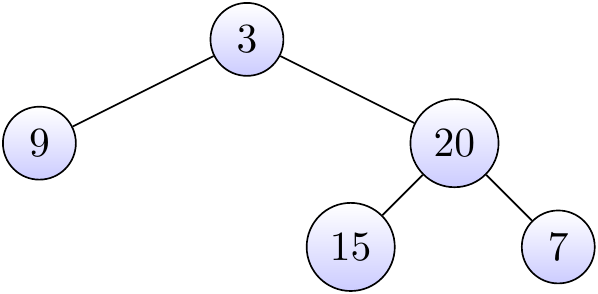
\includegraphics[width=0.9\linewidth]{tech-interview_files/figure-latex/unnamed-chunk-42-1} \caption{Some caption.}\label{fig:unnamed-chunk-42}
\end{figure}

\hypertarget{solution-56}{%
\subsection{Solution}\label{solution-56}}

\hypertarget{walkthrough-90}{%
\subsubsection{Walkthrough\textbackslash{}}\label{walkthrough-90}}

PreOrder array is used to construct data value of a node, whereas InOrder array is used to acknowledge the left and right boundary
of a node. We could use a Map to store the InOrder array associated with its index (position in array) value and biuld
tree according to the following conditions:

\begin{itemize}
\tightlist
\item
  if startIdx \(>\) endIdx Return null. (Terminal)
\item
  if startIdx \(==\) endIdx The node is here. (Terminal)
\item
  if startIdx \(>\) endIdx There should be more nodes in this branch.
\end{itemize}

\hypertarget{analysis-97}{%
\subsubsection{Analysis\textbackslash{}}\label{analysis-97}}

Time complexity is O(n) as every node is visited once.

\hypertarget{algorithm-99}{%
\subsubsection{Algorithm\textbackslash{}}\label{algorithm-99}}

dfs \ref{dfs}

\hypertarget{java-code---preorder-recursive-1}{%
\subsection{Java Code - PreOrder Recursive}\label{java-code---preorder-recursive-1}}

\begin{Shaded}
\begin{Highlighting}[]
\DataTypeTok{int}\NormalTok{ preorderIndex = }\DecValTok{0}\NormalTok{;}

\KeywordTok{public} \BuiltInTok{TreeNode} \FunctionTok{buildTree}\NormalTok{(}\DataTypeTok{int}\NormalTok{[] preorder, }\DataTypeTok{int}\NormalTok{[] inorder) \{}
    \KeywordTok{if}\NormalTok{ (preorder.}\FunctionTok{length}\NormalTok{ == }\DecValTok{0}\NormalTok{) \{}
        \KeywordTok{return} \KeywordTok{null}\NormalTok{;}
\NormalTok{    \}}

    \BuiltInTok{Map}\NormalTok{<}\BuiltInTok{Integer}\NormalTok{, }\BuiltInTok{Integer}\NormalTok{> inorderIndex = }\KeywordTok{new} \BuiltInTok{HashMap}\NormalTok{<>();}
    \KeywordTok{for}\NormalTok{ (}\DataTypeTok{int}\NormalTok{ i = }\DecValTok{0}\NormalTok{; i < inorder.}\FunctionTok{length}\NormalTok{; i++) \{}
\NormalTok{        inorderIndex.}\FunctionTok{put}\NormalTok{(inorder[i], i);}
\NormalTok{    \}}

    \KeywordTok{return} \FunctionTok{buildTree}\NormalTok{(preorder, inorderIndex, }\DecValTok{0}\NormalTok{, inorder.}\FunctionTok{length}\NormalTok{ - }\DecValTok{1}\NormalTok{);}
\NormalTok{\}}

\KeywordTok{private} \BuiltInTok{TreeNode} \FunctionTok{buildTree}\NormalTok{(}\DataTypeTok{int}\NormalTok{[] preorder, }\BuiltInTok{Map}\NormalTok{<}\BuiltInTok{Integer}\NormalTok{, }\BuiltInTok{Integer}\NormalTok{> inorderIndex, }\DataTypeTok{int}\NormalTok{ startIdx, }\DataTypeTok{int}\NormalTok{ endIdx) \{}
    \KeywordTok{if}\NormalTok{ (startIdx > endIdx) \{}
        \KeywordTok{return} \KeywordTok{null}\NormalTok{;}
\NormalTok{    \}}

    \DataTypeTok{int}\NormalTok{ val = preorder[preorderIndex++];}
    \BuiltInTok{TreeNode}\NormalTok{ node = }\KeywordTok{new} \BuiltInTok{TreeNode}\NormalTok{(val);}

    \KeywordTok{if}\NormalTok{ (startIdx == endIdx) \{}
        \KeywordTok{return}\NormalTok{ node;}
\NormalTok{    \}}

    \DataTypeTok{int}\NormalTok{ inIndex = inorderIndex.}\FunctionTok{get}\NormalTok{(val);}
\NormalTok{    node.}\FunctionTok{left}\NormalTok{ = }\FunctionTok{buildTree}\NormalTok{(preorder, inorderIndex, startIdx, inIndex - }\DecValTok{1}\NormalTok{);}
\NormalTok{    node.}\FunctionTok{right}\NormalTok{ = }\FunctionTok{buildTree}\NormalTok{(preorder, inorderIndex, inIndex + }\DecValTok{1}\NormalTok{, endIdx);}

    \KeywordTok{return}\NormalTok{ node;}
\NormalTok{\}}
\end{Highlighting}
\end{Shaded}

\hypertarget{graph}{%
\chapter{Graph}\label{graph}}

Imagine a graph with as the following:

\begin{verbatim}
1 -- 0 -- 4
|
5 -- 6
|  / | \
| /  |   \
2 -- 3 -- 7
\end{verbatim}

\subsubsection{Typical Implementation - Adjacency List}

An adjacency list is created with an array of lists. Size of the array is equal to the number of vertices. Each entry
represents the list of vertices adjacent to the \(i^{th}\) vertex. Each node maintains a list of all its adjacent edges,
then, for each node, you could discover all its neighbors by traversing its adjacency list just once in linear time.

\begin{verbatim}
| 0 | -- 1 -- 4
| 1 | -- 0 -- 5
| 2 | -- 3 -- 5 -- 6
| 3 | -- 2 -- 6 -- 7
| 4 | -- 0
| 5 | -- 1 -- 2 -- 6
| 6 | -- 2 -- 3 -- 5 -- 7
| 7 | -- 3 -- 6
\end{verbatim}

\subsubsection{Typical Implementation - Adjacency Matrix}

The adjacency information can also transform into matrix form with the convention followed here (for undirected graphs)
is that each edge adds 1 to the appropriate cell in the matrix, and each loop adds 2. For each node, you have to
traverse an entire row of length V in the matrix to discover all its outgoing edges.

\begin{verbatim}
0, 1, 0, 0, 1, 0, 0, 0
1, 0, 0, 0, 0, 1, 0, 0
0, 0, 0, 1, 0, 1, 1, 0
0, 0, 1, 0, 0, 0, 1, 1
1, 0, 0, 0, 0, 0, 0, 0
0, 1, 1, 0, 0, 0, 1, 0
0, 0, 1, 1, 0, 1, 0, 1
0, 0, 0, 1, 0, 0, 1, 0
\end{verbatim}

In addition, a ``visited'' array that we'll use to keep track of which vertices have been visited.

\subsubsection{Typical Implementation - Graph based}

\begin{Shaded}
\begin{Highlighting}[]
\KeywordTok{class}\NormalTok{ Graph  \{}
    \KeywordTok{private} \DataTypeTok{int}\NormalTok{ numOfVertices;   }\CommentTok{//No. of vertices}
    \KeywordTok{private} \BuiltInTok{List}\NormalTok{<}\BuiltInTok{Integer}\NormalTok{> adj[]; }\CommentTok{//Adjacency List}
    \KeywordTok{private} \DataTypeTok{boolean}\NormalTok{[] visited;   }\CommentTok{//visited mark for each vertex}

    \CommentTok{// Constructor}
    \KeywordTok{public} \FunctionTok{Graph}\NormalTok{(}\DataTypeTok{int}\NormalTok{ num) \{}
\NormalTok{        numOfVertices = num;}
\NormalTok{        adj = }\KeywordTok{new} \BuiltInTok{LinkedList}\NormalTok{[v];}
        \KeywordTok{for}\NormalTok{ (}\DataTypeTok{int}\NormalTok{ i=}\DecValTok{0}\NormalTok{; i<numOfVertices; ++i) \{}
\NormalTok{            adj[i] = }\KeywordTok{new} \BuiltInTok{LinkedList}\NormalTok{();}
\NormalTok{        \}}
\NormalTok{    \}}
\NormalTok{    ...}
\NormalTok{\}}
\end{Highlighting}
\end{Shaded}

There is an alternative implementation to represent per node with a list of adjacent nodes.

\subsubsection{Typical Implementation - per Node based}

\begin{Shaded}
\begin{Highlighting}[]
\KeywordTok{class} \BuiltInTok{Node}\NormalTok{ \{}
    \KeywordTok{public} \DataTypeTok{int}\NormalTok{ val;}
    \KeywordTok{public} \BuiltInTok{List}\NormalTok{<}\BuiltInTok{Node}\NormalTok{> neighbors;}
    \KeywordTok{private} \DataTypeTok{boolean}\NormalTok{ visited;     }\CommentTok{//visited mark for the vertex}

    \KeywordTok{public} \BuiltInTok{Node}\NormalTok{(}\DataTypeTok{int}\NormalTok{ _val, }\BuiltInTok{List}\NormalTok{<}\BuiltInTok{Node}\NormalTok{> _neighbors) \{}
\NormalTok{        val = _val;}
\NormalTok{        neighbors = _neighbors;}
\NormalTok{    \}}
\NormalTok{    ...}
\NormalTok{\}}
\end{Highlighting}
\end{Shaded}

\hypertarget{depth-first-traversal-1}{%
\subsection{Depth First Traversal}\label{depth-first-traversal-1}}

A depth first traversal without labeling the visited node usually ends up in exponential time complexity. There will be
many subproblems being reevaluated (which were visited in past). Thus, the time complexity is \(O(2^{h+1} - 1)\) (as a
full binary tree)

If your graph is implemented as an adjacency matrix, then, for each node, you have to traverse an entire row of length
V in the matrix to discover all its outgoing edges. So, the complexity of DFS is \(O(|V| * |V|) = O(|V|^2)\).

If your graph is implemented using adjacency lists, wherein each node maintains a list of all its adjacent edges,
then, for each node, you could discover all its neighbors by traversing its adjacency list just once in linear time.
For a directed graph, the sum of the sizes of the adjacency lists of all the nodes is E (total number of edges). So, the
complexity of DFS is O(V) + O(E) = O(V + E). For an undirected graph, each edge will appear twice. Once in the adjacency
list of either end of the edge. So, the overall complexity will be \(O(|V|) + O (2\cdot |E|) = O(|V + E|)\).

\hypertarget{algorithm-100}{%
\subsubsection{Algorithm\textbackslash{}}\label{algorithm-100}}

dfs \ref{dfs}

\subsubsection{Typical Implementation - Java}

\begin{Shaded}
\begin{Highlighting}[]
\DataTypeTok{void} \FunctionTok{helper}\NormalTok{(}\DataTypeTok{int}\NormalTok{ node, }\DataTypeTok{boolean}\NormalTok{ visited[]) \{}
    \CommentTok{// Mark the current node as visited and print it}
\NormalTok{    visited[node] = }\KeywordTok{true}\NormalTok{;}

    \CommentTok{// Recur for all the vertices adjacent to this vertex}
    \KeywordTok{for}\NormalTok{(}\BuiltInTok{Integer}\NormalTok{ adjNode: adj[node]) \{}
        \KeywordTok{if}\NormalTok{ (!visited[adjNode]) \{}
            \FunctionTok{helper}\NormalTok{(adjNode, visited);}
\NormalTok{        \}}
\NormalTok{    \}}
\NormalTok{\}}

\CommentTok{// The function to do DFS traversal. It uses recursive DFSUtil()}
\DataTypeTok{void} \FunctionTok{dfs}\NormalTok{(}\DataTypeTok{int}\NormalTok{ root) \{}
    \CommentTok{// Mark all the vertices as not visited(set as}
    \CommentTok{// false by default in java)}
    \DataTypeTok{boolean}\NormalTok{ visited[] = }\KeywordTok{new} \DataTypeTok{boolean}\NormalTok{[numOfVertices];}

    \FunctionTok{helper}\NormalTok{(root, visited);}
\NormalTok{\}}
\end{Highlighting}
\end{Shaded}

\hypertarget{bread-first-traversal}{%
\subsection{Bread First Traversal}\label{bread-first-traversal}}

For every single vertex in the graph, we will end up looking at its neighboring nodes only once (directed graph) or
twice (undirected graph). The time complexity for both a directed and undirected graph is the sum of the vertices and
their edges as represented by the graph in its adjacency list representation, or \(O(|V| + |E|)\)

The power of using breadth-first search to traverse through a graph is that it can easily tell us the shortest way to
get from one node to another.

\hypertarget{algorithm-101}{%
\subsubsection{Algorithm\textbackslash{}}\label{algorithm-101}}

bfs \ref{bfs}

\subsubsection{Typical Implementation - Java}

\begin{Shaded}
\begin{Highlighting}[]
\KeywordTok{class}\NormalTok{ Graph  \{}
    \KeywordTok{private} \DataTypeTok{int}\NormalTok{ numOfVertices;   }\CommentTok{// No. of vertices}
    \KeywordTok{private} \BuiltInTok{LinkedList}\NormalTok{<}\BuiltInTok{Integer}\NormalTok{> adj[]; }\CommentTok{//Adjacency Lists}

\NormalTok{    ...}

    \DataTypeTok{void} \FunctionTok{traversal}\NormalTok{(}\BuiltInTok{Integer}\NormalTok{ root)  \{}
        \CommentTok{// Mark all the vertices as not visited(By default}
        \CommentTok{// set as false)}
        \DataTypeTok{boolean}\NormalTok{ visited[] = }\KeywordTok{new} \DataTypeTok{boolean}\NormalTok{[numOfVertices];}

        \CommentTok{// Create a queue for BFS}
        \BuiltInTok{Queue}\NormalTok{<}\BuiltInTok{Integer}\NormalTok{> queue = }\KeywordTok{new} \BuiltInTok{LinkedList}\NormalTok{<}\BuiltInTok{Integer}\NormalTok{>();}

        \CommentTok{// Mark the current node as visited and enqueue it}
\NormalTok{        visited[root] = }\KeywordTok{true}\NormalTok{;}
\NormalTok{        queue.}\FunctionTok{offer}\NormalTok{(root);}

        \KeywordTok{while}\NormalTok{ (queue.}\FunctionTok{size}\NormalTok{() != }\DecValTok{0}\NormalTok{) \{}
            \CommentTok{// Dequeue a vertex from queue and print it}
            \BuiltInTok{Integer}\NormalTok{ node = queue.}\FunctionTok{poll}\NormalTok{();}

            \CommentTok{// Get all adjacent vertices of the dequeued vertex s}
            \CommentTok{// If a adjacent has not been visited, then mark it}
            \CommentTok{// visited and enqueue it}
            \KeywordTok{for}\NormalTok{(}\BuiltInTok{Integer}\NormalTok{ adjNode : adj[node]) \{}
                \KeywordTok{if}\NormalTok{ (!visited[adjNode] && !queue.}\FunctionTok{contain}\NormalTok{(adjNode)) \{}
\NormalTok{                    queue.}\FunctionTok{offer}\NormalTok{(adjNode);}
\NormalTok{                \}}
\NormalTok{            \}}
\NormalTok{        \}}
\NormalTok{    \}}
\NormalTok{\}}
\end{Highlighting}
\end{Shaded}

\hypertarget{topological-sorting}{%
\subsection{Topological Sorting}\label{topological-sorting}}

A traversal algorithm for \textbf{Directed Acyclic Graph (DAG)} is a linear ordering of vertices such that for every
directed edge \([u,v]\), vertex u comes before v in the ordering.

\subsubsection{By DFS}

In DFS implementation of Topological Sort we focused on sink vertices, i.e, vertices with zero out-going edges, and then
at last had to reverse the order in which we got the \textbf{sink vertices} (which we did by using a stack, which is a
Last In First Out data structure). A DAG has to have at least one sink vertex which is the vertex which has no outbound
edges. In DFS we print the nodes as we see them, which means when we print a node, it has just been discovered but not
yet processed, which means it is in the Visiting state. So DFS gives the order in which the nodes enter the Visiting
state and not the Visited state. For topological sorting we need to have the order in which the nodes are completely
processed, i.e, the order in which the nodes are marked as Visited. Because when a node is marked Visited then all of
its child node have already been processed, so they would be towards the right of the child nodes in the topological
sort, as it should be.

For example, in the given graph, the vertex `5' should be printed before vertex `0', but unlike DFS, the vertex `4'
should also be printed before vertex `0'.

\begin{verbatim}
5 -> 0 <- 4
|         |
v         v
2 -> 3 -> 1
\end{verbatim}

In topological sorting, we use a temporary stack. We don't print the vertex immediately, we first recursively call
topological sorting for all its adjacent vertices, then push it to a stack. Finally, print contents of stack. The
final sequence is {[}5, 4, 2, 3, 1, 0{]}

\hypertarget{algorithm-102}{%
\subsubsection{Algorithm\textbackslash{}}\label{algorithm-102}}

\begin{verbatim}
topological \\ref{topological}, dfs \\ref{dfs}
\end{verbatim}

\subsubsection{Typical Implementation - Java Code}

\begin{Shaded}
\begin{Highlighting}[]
\DataTypeTok{void} \FunctionTok{helper}\NormalTok{(}\BuiltInTok{Integer}\NormalTok{ v, }\BuiltInTok{Stack}\NormalTok{ stack) \{}
\NormalTok{    visited[v] = }\KeywordTok{true}\NormalTok{;}

    \CommentTok{// Recur for all the vertices adjacent to this}
    \CommentTok{// vertex}
    \BuiltInTok{Iterator}\NormalTok{<}\BuiltInTok{Integer}\NormalTok{> it = adj[v].}\FunctionTok{iterator}\NormalTok{();}
    \KeywordTok{while}\NormalTok{ (it.}\FunctionTok{hasNext}\NormalTok{()) \{}
        \BuiltInTok{Integer}\NormalTok{ adjNode = it.}\FunctionTok{next}\NormalTok{();}

        \KeywordTok{if}\NormalTok{ (!visited[adjNode])  \{}
            \FunctionTok{helper}\NormalTok{(adjNode, visited, stack);}
\NormalTok{        \}}
\NormalTok{    \}}

    \CommentTok{// Push current vertex to stack which stores result}
\NormalTok{    stack.}\FunctionTok{push}\NormalTok{(}\KeywordTok{new} \BuiltInTok{Integer}\NormalTok{(v));}
\NormalTok{\}}

\BuiltInTok{List}\NormalTok{<}\BuiltInTok{Integer}\NormalTok{> }\FunctionTok{topologicalSort}\NormalTok{(Graph graph) \{}
    \BuiltInTok{Stack}\NormalTok{<}\BuiltInTok{Integer}\NormalTok{> stack = }\KeywordTok{new} \BuiltInTok{Stack}\NormalTok{<>();}
    \BuiltInTok{List}\NormalTok{<}\BuiltInTok{Integer}\NormalTok{> result = }\KeywordTok{new} \BuiltInTok{ArrayList}\NormalTok{<>();}

    \CommentTok{// Call the recursive helper function to store}
    \CommentTok{// Topological Sort starting from all vertices}
    \CommentTok{// one by one}
    \KeywordTok{for}\NormalTok{ (}\DataTypeTok{int}\NormalTok{ i = }\DecValTok{0}\NormalTok{; i < numOfVertices; i++) \{}
        \KeywordTok{if}\NormalTok{ (visited[i] == }\KeywordTok{false}\NormalTok{)  \{}
            \FunctionTok{helper}\NormalTok{(i, visited, stack);}
\NormalTok{        \}}
\NormalTok{    \}}

    \CommentTok{//Now the stack contains the topological sorting of the graph}
    \KeywordTok{for}\NormalTok{ (}\BuiltInTok{Integer}\NormalTok{ vertex : stack) \{}
\NormalTok{        result.}\FunctionTok{add}\NormalTok{(stack.}\FunctionTok{pop}\NormalTok{());}
\NormalTok{    \}}

    \KeywordTok{return}\NormalTok{ result}
\NormalTok{\}}
\end{Highlighting}
\end{Shaded}

\subsubsection{By BFS}

In BFS implementation of the Topological sort we do the opposite: We look for for edges with no inbound edges
(\textbf{source vertex}). And consequently in BFS implementation we don't have to reverse the order in which we get the
vertices, since we get the vertices in order of the topological ordering. We use First-In-First-Out data structure
Queue in this implementation. We just search for the vertices with zero indegrees and put them in the queue till
we have processed all the vertices of the graph. Polling vertices from the queue one by one give the topological sort
of the graph. Lastly check if the result set does not contain all the vertices that means there is at least one cycle
in the graph. That is because the indegree of those vertices participating in the loop could not be made 0 by
decrementing.

\begin{figure}
\centering
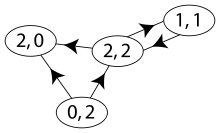
\includegraphics{img/graph_dag_degrees.png}
\caption{in-degree, out-degree}
\end{figure}

\hypertarget{algorithm-103}{%
\subsubsection{Algorithm\textbackslash{}}\label{algorithm-103}}

topological \ref{topological}, bfs \ref{bfs}

\subsubsection{Typical Implementation - Java Code}

\begin{Shaded}
\begin{Highlighting}[]
\KeywordTok{public} \BuiltInTok{List} \FunctionTok{topological_sort_bfs}\NormalTok{(}\DataTypeTok{int}\NormalTok{[][] graph) \{}
    \BuiltInTok{List}\NormalTok{<}\BuiltInTok{Integer}\NormalTok{> result = }\KeywordTok{new} \BuiltInTok{ArrayList}\NormalTok{<>();}
    \DataTypeTok{int}\NormalTok{[] indegree = }\KeywordTok{new} \DataTypeTok{int}\NormalTok{[numOfVertices];}

    \CommentTok{// compute the indegree of all the vertices in the graph}
    \CommentTok{// For edge (0,1), indegree[1]++;}
    \KeywordTok{for}\NormalTok{ (}\DataTypeTok{int}\NormalTok{ i = }\DecValTok{0}\NormalTok{; i < numOfVertices; i++) \{}
        \KeywordTok{for}\NormalTok{(}\BuiltInTok{Integer}\NormalTok{ vertex : adj[i]) \{}
\NormalTok{            indegree[vertex]++;}
\NormalTok{        \}}
\NormalTok{    \}}

    \BuiltInTok{Queue}\NormalTok{<}\BuiltInTok{Integer}\NormalTok{> queue = }\KeywordTok{new} \BuiltInTok{LinkedList}\NormalTok{<>();}

    \CommentTok{// initialize the queue with all the vertices with no inbound edges}
    \KeywordTok{for}\NormalTok{ (}\BuiltInTok{Integer}\NormalTok{ vertex = }\DecValTok{0}\NormalTok{; index < numOfVertices; index++) \{}
        \KeywordTok{if}\NormalTok{ (indegree[vertex] == }\DecValTok{0}\NormalTok{) \{}
\NormalTok{            queue.}\FunctionTok{offer}\NormalTok{(vertex);}
\NormalTok{        \}}
\NormalTok{    \}}

    \KeywordTok{while}\NormalTok{ (!queue.}\FunctionTok{isEmpty}\NormalTok{()) \{}
        \BuiltInTok{Integer}\NormalTok{ vertex = queue.}\FunctionTok{poll}\NormalTok{();}
\NormalTok{        result.}\FunctionTok{add}\NormalTok{(vertex);}

        \CommentTok{// now disconnect vertex1 from the graph}
        \CommentTok{// and decrease the indegree of the other end of the edge by 1}
        \KeywordTok{for}\NormalTok{ (}\BuiltInTok{Integer}\NormalTok{ adjVertex : adj[i]) \{}
\NormalTok{            indegree[adjVertex]--;}
            \KeywordTok{if}\NormalTok{ (indegree[adjVertex] == }\DecValTok{0}\NormalTok{) \{}
\NormalTok{                queue.}\FunctionTok{offer}\NormalTok{(adjVertex);}
\NormalTok{            \}}
\NormalTok{        \}}
\NormalTok{    \}}

    \CommentTok{// check if the graph had a cycle / loop}
    \KeywordTok{if}\NormalTok{ (result.}\FunctionTok{size}\NormalTok{() != numOfVertices) \{}
        \KeywordTok{return} \KeywordTok{new} \BuiltInTok{ArrayList}\NormalTok{<}\BuiltInTok{Integer}\NormalTok{>();}
\NormalTok{    \}}
    \KeywordTok{return}\NormalTok{ result;}
\NormalTok{\}}
\end{Highlighting}
\end{Shaded}

\hypertarget{graph-serialization}{%
\section{Graph Serialization / /}\label{graph-serialization}}

\hypertarget{description-80}{%
\subsection{Description}\label{description-80}}

Given the a node to a Graph, represent that Graph as a String in such a way that it may be translated back to a
Graph using the generated String A Node contains an integer value and all of the node's neighbors.
\#\#\# Example
N.A.

\hypertarget{solution-57}{%
\subsection{Solution}\label{solution-57}}

\hypertarget{walkthrough-91}{%
\subsubsection{Walkthrough\textbackslash{}}\label{walkthrough-91}}

We use BFS to traverse the graph with a visited Set to avoid running into cycle, and add child node only on unvisited
adjacent nodes. For serialization, we simply place current val as first element and adjacent nodes val at the same
line for the following elements, i.e.~current, adj1, adj2, adj3, ..etc. Therefore, there will be two occurrence
for each node-pair (edges) in the serialized content. For deserialization, it is easier by first splitting the lines
and splitting by the dilimter `,' and finally reassemble the graph data structure.

\hypertarget{analysis-98}{%
\subsubsection{Analysis\textbackslash{}}\label{analysis-98}}

The time complexity for both a directed and undirected graph is the sum of the vertices and
their edges as represented by the graph in its adjacency list representation, or \(O(|V| + |E|)\)

\begin{Shaded}
\begin{Highlighting}[]
\NormalTok{Graph:}
\DecValTok{1}
\NormalTok{Serialized Content:}
\DecValTok{1}
\end{Highlighting}
\end{Shaded}

\begin{Shaded}
\begin{Highlighting}[]
\NormalTok{Graph:}
\DecValTok{1}\NormalTok{ - }\DecValTok{2}
\NormalTok{|   |}
\DecValTok{3}\NormalTok{ - }\DecValTok{5}
\NormalTok{|}
\DecValTok{4}
\NormalTok{Serialized Content:}
\DecValTok{1}\NormalTok{, }\DecValTok{2}\NormalTok{, }\DecValTok{3}
\DecValTok{2}\NormalTok{, }\DecValTok{1}\NormalTok{, }\DecValTok{5}
\DecValTok{3}\NormalTok{, }\DecValTok{1}\NormalTok{, }\DecValTok{5}\NormalTok{, }\DecValTok{4}
\DecValTok{4}\NormalTok{, }\DecValTok{3}
\DecValTok{5}\NormalTok{, }\DecValTok{2}\NormalTok{, }\DecValTok{3}
\end{Highlighting}
\end{Shaded}

\hypertarget{algorithm-104}{%
\subsubsection{Algorithm\textbackslash{}}\label{algorithm-104}}

bfs \ref{bfs}

\hypertarget{java-code-59}{%
\subsection{Java Code}\label{java-code-59}}

\begin{Shaded}
\begin{Highlighting}[]
\KeywordTok{class}\NormalTok{ Graph \{}
    \KeywordTok{private} \DataTypeTok{int}\NormalTok{ numOfVertices; }\CommentTok{// No. of vertices}
    \KeywordTok{private} \BuiltInTok{LinkedList}\NormalTok{<}\BuiltInTok{Integer}\NormalTok{> adj[]; }\CommentTok{//Adjacency Lists}

    \CommentTok{// Constructor}
    \FunctionTok{Graph}\NormalTok{(}\DataTypeTok{int}\NormalTok{ num) \{}
\NormalTok{        numOfVertices = num;}
\NormalTok{        adj = }\KeywordTok{new} \BuiltInTok{LinkedList}\NormalTok{[numOfVertices];}
        \KeywordTok{for}\NormalTok{ (}\DataTypeTok{int}\NormalTok{ i = }\DecValTok{0}\NormalTok{; i < numOfVertices; ++i) \{}
\NormalTok{            adj[i] = }\KeywordTok{new} \BuiltInTok{LinkedList}\NormalTok{();}
\NormalTok{        \}}
\NormalTok{    \}}

    \CommentTok{// Function to add an edge into the graph from v1 to v2}
    \KeywordTok{public} \DataTypeTok{void} \FunctionTok{addEdge}\NormalTok{(}\DataTypeTok{int}\NormalTok{ v1, }\DataTypeTok{int}\NormalTok{ v2) \{}
\NormalTok{        adj[v1].}\FunctionTok{add}\NormalTok{(v2);}
\NormalTok{    \}}

    \KeywordTok{public} \BuiltInTok{String} \FunctionTok{serialize}\NormalTok{(}\BuiltInTok{Integer}\NormalTok{ rootId) \{}
        \BuiltInTok{StringBuilder}\NormalTok{ stringBuilder = }\KeywordTok{new} \BuiltInTok{StringBuilder}\NormalTok{();}

        \KeywordTok{if}\NormalTok{(adj.}\FunctionTok{length}\NormalTok{ <= }\DecValTok{0}\NormalTok{) \{}
            \KeywordTok{return} \StringTok{""}\NormalTok{;}
\NormalTok{        \}}

        \DataTypeTok{boolean}\NormalTok{ visited[] = }\KeywordTok{new} \DataTypeTok{boolean}\NormalTok{[numOfVertices];}
        \BuiltInTok{Queue}\NormalTok{<}\BuiltInTok{Integer}\NormalTok{> queue = }\KeywordTok{new} \BuiltInTok{LinkedList}\NormalTok{<}\BuiltInTok{Integer}\NormalTok{>();}

        \CommentTok{// Mark the current node as visited and enqueue it}
\NormalTok{        queue.}\FunctionTok{offer}\NormalTok{(rootId);}

        \KeywordTok{while}\NormalTok{ (queue.}\FunctionTok{size}\NormalTok{() != }\DecValTok{0}\NormalTok{) \{}
            \BuiltInTok{Integer}\NormalTok{ nodeId = queue.}\FunctionTok{poll}\NormalTok{();}
\NormalTok{            visited[nodeId]=}\KeywordTok{true}\NormalTok{;}

\NormalTok{            stringBuilder.}\FunctionTok{append}\NormalTok{(}\FunctionTok{serializeNode}\NormalTok{(nodeId));}

            \CommentTok{// Get all adjacent vertices of the dequeued vertex s}
            \CommentTok{// If a adjacent has not been visited, then mark it}
            \CommentTok{// visited and enqueue it}
            \KeywordTok{for}\NormalTok{(}\BuiltInTok{Integer}\NormalTok{ adjNodeId : adj[nodeId]) \{}
                \KeywordTok{if}\NormalTok{ (!visited[adjNodeId] && !queue.}\FunctionTok{contains}\NormalTok{(adjNodeId)) \{}
\NormalTok{                    queue.}\FunctionTok{offer}\NormalTok{(adjNodeId);}
\NormalTok{                \}}
\NormalTok{            \}}
\NormalTok{        \}}

        \KeywordTok{return}\NormalTok{ stringBuilder.}\FunctionTok{toString}\NormalTok{();}
\NormalTok{    \}}

    \KeywordTok{private} \BuiltInTok{String} \FunctionTok{serializeNode}\NormalTok{(}\DataTypeTok{int}\NormalTok{ nodeId) \{}
        \BuiltInTok{StringBuilder}\NormalTok{ sb = }\KeywordTok{new} \BuiltInTok{StringBuilder}\NormalTok{();}

        \CommentTok{//serialize node and adjacency nodes}
\NormalTok{        sb.}\FunctionTok{append}\NormalTok{(nodeId);}
        \KeywordTok{for}\NormalTok{(}\BuiltInTok{Integer}\NormalTok{ adjNodeId: adj[nodeId]) \{}
\NormalTok{            sb.}\FunctionTok{append}\NormalTok{(}\StringTok{","}\NormalTok{);}
\NormalTok{            sb.}\FunctionTok{append}\NormalTok{(adjNodeId);}
\NormalTok{        \}}
\NormalTok{        sb.}\FunctionTok{append}\NormalTok{(}\StringTok{"}\SpecialCharTok{\textbackslash{}r\textbackslash{}n}\StringTok{"}\NormalTok{);}

        \KeywordTok{return}\NormalTok{ sb.}\FunctionTok{toString}\NormalTok{();}
\NormalTok{    \}}

    \KeywordTok{public}\NormalTok{ Graph }\FunctionTok{deserialize}\NormalTok{(}\BuiltInTok{String}\NormalTok{ input) \{}
        \BuiltInTok{String}\NormalTok{[] lines = input.}\FunctionTok{split}\NormalTok{(}\StringTok{"}\SpecialCharTok{\textbackslash{}r\textbackslash{}n}\StringTok{"}\NormalTok{);}
\NormalTok{        Graph graph = }\KeywordTok{new} \FunctionTok{Graph}\NormalTok{(lines.}\FunctionTok{length}\NormalTok{);}

        \KeywordTok{for}\NormalTok{(}\BuiltInTok{String}\NormalTok{ line: lines) \{}
            \BuiltInTok{String}\NormalTok{[] nodes = line.}\FunctionTok{split}\NormalTok{(}\StringTok{","}\NormalTok{);}

            \KeywordTok{if}\NormalTok{(nodes.}\FunctionTok{length}\NormalTok{ > }\DecValTok{1}\NormalTok{) \{}
                \DataTypeTok{int}\NormalTok{ srcNodeId = }\BuiltInTok{Integer}\NormalTok{.}\FunctionTok{parseInt}\NormalTok{(nodes[}\DecValTok{0}\NormalTok{]);}

                \CommentTok{//there are adjacent nodes}
                \KeywordTok{for}\NormalTok{(}\DataTypeTok{int}\NormalTok{ j = }\DecValTok{1}\NormalTok{; j < nodes.}\FunctionTok{length}\NormalTok{; j++) \{}
                    \BuiltInTok{Integer}\NormalTok{ dstNodeId = }\BuiltInTok{Integer}\NormalTok{.}\FunctionTok{valueOf}\NormalTok{(nodes[j]);}
\NormalTok{                    graph.}\FunctionTok{addEdge}\NormalTok{(srcNodeId, dstNodeId);}
\NormalTok{                \}}
\NormalTok{            \}}
\NormalTok{        \}}

        \KeywordTok{return}\NormalTok{ graph;}
\NormalTok{    \}}
\NormalTok{\}}
\end{Highlighting}
\end{Shaded}

\hypertarget{distance-of-nearest-cell-having-1-in-a-binary-matrix}{%
\section{Distance of nearest cell having 1 in a binary matrix}\label{distance-of-nearest-cell-having-1-in-a-binary-matrix}}

\hypertarget{description-81}{%
\subsection{Description}\label{description-81}}

Given a binary matrix of N x M, containing at least a value 1. The task is to find the distance of nearest 1 in the
matrix for each cell. The distance is calculated as \(|i_1 - i_2| + |j_1 - j_2|\), where \(i_1, j_1\) are the row number
and column number of the current cell and \(i_2, j_2\) are the row number and column number of the nearest cell having
value 1.

\hypertarget{example-77}{%
\subsection{Example}\label{example-77}}

Input:

\begin{Shaded}
\begin{Highlighting}[]
\DecValTok{0}\NormalTok{, }\DecValTok{0}\NormalTok{, }\DecValTok{0}\NormalTok{, }\DecValTok{1}
\DecValTok{0}\NormalTok{, }\DecValTok{0}\NormalTok{, }\DecValTok{1}\NormalTok{, }\DecValTok{1}
\DecValTok{0}\NormalTok{, }\DecValTok{1}\NormalTok{, }\DecValTok{1}\NormalTok{, }\DecValTok{0}
\end{Highlighting}
\end{Shaded}

Output:

\begin{Shaded}
\begin{Highlighting}[]
\DecValTok{3}\NormalTok{, }\DecValTok{2}\NormalTok{, }\DecValTok{1}\NormalTok{, }\DecValTok{0}
\DecValTok{2}\NormalTok{, }\DecValTok{1}\NormalTok{, }\DecValTok{0}\NormalTok{, }\DecValTok{0}
\DecValTok{1}\NormalTok{, }\DecValTok{0}\NormalTok{, }\DecValTok{0}\NormalTok{, }\DecValTok{1}
\end{Highlighting}
\end{Shaded}

\hypertarget{solution-58}{%
\subsection{Solution}\label{solution-58}}

\hypertarget{walkthrough-92}{%
\subsubsection{Walkthrough\textbackslash{}}\label{walkthrough-92}}

Consider each cell as a node and each boundary between any two adjacent cells be an edge. Number each cell from 1 to
N*M. Now, push all the node whose corresponding cell value is 1 in the matrix in the queue. Apply BFS using this queue
to find the minimum distance of the adjacent node.

\hypertarget{analysis-99}{%
\subsubsection{Analysis\textbackslash{}}\label{analysis-99}}

\begin{verbatim}
*  Create a graph with adjacency list for all nodes from 1 to rows * cols. Time complexity is O(rows * cols)
*  Create an empty queue and 1 dimensional array of size (rows * cols) for visited[] and distance (init Integer.MAX)
\end{verbatim}

Time complexity is O(rows * cols)
* For all nodes in the original matrix being 1, insert the associated node id into the queue and set the
distance to 0.
* Perform a BFS traversal of graph using above created queue. In BFS, we first explore immediate adjacent of all
1's, then adjacent of adjacent and determine the minimum distance. Time complexity is O(rows * cols) since all elements
will be visited once.

Thus, the overall time complexity is O(rows * cols)

\hypertarget{algorithm-105}{%
\subsubsection{Algorithm\textbackslash{}}\label{algorithm-105}}

bfs \ref{bfs}

\hypertarget{java-code-60}{%
\subsection{Java Code}\label{java-code-60}}

\begin{Shaded}
\begin{Highlighting}[]
\KeywordTok{class}\NormalTok{ Graph \{}
    \KeywordTok{private} \DataTypeTok{int}\NormalTok{ numOfVertices; }\CommentTok{// No. of vertices}
    \KeywordTok{private} \BuiltInTok{LinkedList}\NormalTok{<}\BuiltInTok{Integer}\NormalTok{> adj[]; }\CommentTok{//Adjacency Lists}

    \CommentTok{// Constructor}
    \FunctionTok{Graph}\NormalTok{(}\DataTypeTok{int}\NormalTok{[][] matrix) \{}
        \DataTypeTok{int}\NormalTok{ rows = matrix.}\FunctionTok{length}\NormalTok{;}
        \DataTypeTok{int}\NormalTok{ cols = matrix[}\DecValTok{0}\NormalTok{].}\FunctionTok{length}\NormalTok{;}

        \KeywordTok{if}\NormalTok{(matrix.}\FunctionTok{length}\NormalTok{ == }\DecValTok{0}\NormalTok{) \{}
            \KeywordTok{return}\NormalTok{;}
\NormalTok{        \}}
\NormalTok{        numOfVertices = rows * cols;}
\NormalTok{        adj = }\KeywordTok{new} \BuiltInTok{LinkedList}\NormalTok{[numOfVertices];}

        \KeywordTok{for}\NormalTok{ (}\DataTypeTok{int}\NormalTok{ i = }\DecValTok{0}\NormalTok{; i < numOfVertices; ++i) \{}
\NormalTok{            adj[i] = }\KeywordTok{new} \BuiltInTok{LinkedList}\NormalTok{();}
\NormalTok{        \}}
\NormalTok{    \}}

    \CommentTok{// Function to add an edge into the graph from v1 to v2}
    \KeywordTok{public} \DataTypeTok{void} \FunctionTok{addEdge}\NormalTok{(}\DataTypeTok{int}\NormalTok{ src, }\DataTypeTok{int}\NormalTok{ dst) \{}
\NormalTok{        adj[src].}\FunctionTok{add}\NormalTok{(dst);}
\NormalTok{    \}}

    \KeywordTok{public} \DataTypeTok{void} \FunctionTok{fillAdjacency}\NormalTok{(}\DataTypeTok{int}\NormalTok{[][] matrix) \{}
        \DataTypeTok{int}\NormalTok{ rows = matrix.}\FunctionTok{length}\NormalTok{;}
        \DataTypeTok{int}\NormalTok{ cols = matrix[}\DecValTok{0}\NormalTok{].}\FunctionTok{length}\NormalTok{;}

        \KeywordTok{for}\NormalTok{(}\DataTypeTok{int}\NormalTok{ i = }\DecValTok{0}\NormalTok{; i < rows; i++) \{}
            \KeywordTok{for}\NormalTok{(}\DataTypeTok{int}\NormalTok{ j = }\DecValTok{0}\NormalTok{; j < cols; j++) \{}
                \DataTypeTok{int}\NormalTok{ srcNodeId = }\KeywordTok{this}\NormalTok{.}\FunctionTok{computeNodeId}\NormalTok{(i, j, cols);}
                \DataTypeTok{int}\NormalTok{ dstNodeId = }\DecValTok{-1}\NormalTok{;}

                \CommentTok{//adding left or right neighbor nodes, if there are any (cols > 1)}
                \KeywordTok{if}\NormalTok{(cols > }\DecValTok{1}\NormalTok{) \{}
                    \KeywordTok{if}\NormalTok{ (j == }\DecValTok{0}\NormalTok{) \{}
\NormalTok{                        dstNodeId = }\KeywordTok{this}\NormalTok{.}\FunctionTok{computeNodeId}\NormalTok{(i, j + }\DecValTok{1}\NormalTok{, cols);}
                        \KeywordTok{this}\NormalTok{.}\FunctionTok{addEdge}\NormalTok{(srcNodeId, dstNodeId);}
\NormalTok{                    \} }\KeywordTok{else} \KeywordTok{if}\NormalTok{ (j == cols - }\DecValTok{1}\NormalTok{) \{}
\NormalTok{                        dstNodeId = }\KeywordTok{this}\NormalTok{.}\FunctionTok{computeNodeId}\NormalTok{(i, j - }\DecValTok{1}\NormalTok{, cols);}
                        \KeywordTok{this}\NormalTok{.}\FunctionTok{addEdge}\NormalTok{(srcNodeId, dstNodeId);}
\NormalTok{                    \} }\KeywordTok{else}\NormalTok{ \{}
\NormalTok{                        dstNodeId = }\KeywordTok{this}\NormalTok{.}\FunctionTok{computeNodeId}\NormalTok{(i, j - }\DecValTok{1}\NormalTok{, cols);}
                        \KeywordTok{this}\NormalTok{.}\FunctionTok{addEdge}\NormalTok{(srcNodeId, dstNodeId);}
\NormalTok{                        dstNodeId = }\KeywordTok{this}\NormalTok{.}\FunctionTok{computeNodeId}\NormalTok{(i, j + }\DecValTok{1}\NormalTok{, cols);}
                        \KeywordTok{this}\NormalTok{.}\FunctionTok{addEdge}\NormalTok{(srcNodeId, dstNodeId);}
\NormalTok{                    \}}
\NormalTok{                \}}

                \CommentTok{//adding above or below neighbor nodes, if there are any (rows > 1)}
                \KeywordTok{if}\NormalTok{(rows > }\DecValTok{1}\NormalTok{) \{}
                    \KeywordTok{if}\NormalTok{ (i == }\DecValTok{0}\NormalTok{) \{}
\NormalTok{                        dstNodeId = }\KeywordTok{this}\NormalTok{.}\FunctionTok{computeNodeId}\NormalTok{(i + }\DecValTok{1}\NormalTok{, j, cols);}
                        \KeywordTok{this}\NormalTok{.}\FunctionTok{addEdge}\NormalTok{(srcNodeId, dstNodeId);}
\NormalTok{                    \} }\KeywordTok{else} \KeywordTok{if}\NormalTok{ (i == rows - }\DecValTok{1}\NormalTok{) \{}
\NormalTok{                        dstNodeId = }\KeywordTok{this}\NormalTok{.}\FunctionTok{computeNodeId}\NormalTok{(i - }\DecValTok{1}\NormalTok{, j, cols);}
                        \KeywordTok{this}\NormalTok{.}\FunctionTok{addEdge}\NormalTok{(srcNodeId, dstNodeId);}
\NormalTok{                    \} }\KeywordTok{else}\NormalTok{ \{}
\NormalTok{                        dstNodeId = }\KeywordTok{this}\NormalTok{.}\FunctionTok{computeNodeId}\NormalTok{(i - }\DecValTok{1}\NormalTok{, j, cols);}
                        \KeywordTok{this}\NormalTok{.}\FunctionTok{addEdge}\NormalTok{(srcNodeId, dstNodeId);}
\NormalTok{                        dstNodeId = }\KeywordTok{this}\NormalTok{.}\FunctionTok{computeNodeId}\NormalTok{(i + }\DecValTok{1}\NormalTok{, j, cols);}
                        \KeywordTok{this}\NormalTok{.}\FunctionTok{addEdge}\NormalTok{(srcNodeId, dstNodeId);}
\NormalTok{                    \}}
\NormalTok{                \}}
\NormalTok{            \}}
\NormalTok{        \}}
\NormalTok{    \}}

    \KeywordTok{private} \DataTypeTok{int} \FunctionTok{computeNodeId}\NormalTok{(}\DataTypeTok{int}\NormalTok{ i, }\DataTypeTok{int}\NormalTok{ j, }\DataTypeTok{int}\NormalTok{ cols) \{}
        \CommentTok{// Example}
        \CommentTok{// [0][0] = 0 * 2 + 0 = 0}
        \CommentTok{// [0][1] = 0 * 2 + 1 = 1}
        \CommentTok{// [1][0] = 1 * 2 + 0 = 2}
        \CommentTok{// [1][1] = 1 * 2 + 1 = 3}
        \KeywordTok{return}\NormalTok{ i * cols + j;}
\NormalTok{    \}}


    \KeywordTok{private} \DataTypeTok{void} \FunctionTok{init}\NormalTok{(}\BuiltInTok{Queue}\NormalTok{<}\BuiltInTok{Integer}\NormalTok{> queue, }\DataTypeTok{int}\NormalTok{[][] matrix, }\DataTypeTok{boolean}\NormalTok{[] visited, }\DataTypeTok{int}\NormalTok{[] dist) \{}
        \CommentTok{//Traverse all matrix elements. If it is a 1, then insert associated node id into queue}
        \KeywordTok{if}\NormalTok{(matrix.}\FunctionTok{length}\NormalTok{ == }\DecValTok{0}\NormalTok{) \{}
            \KeywordTok{return}\NormalTok{;}
\NormalTok{        \}}

        \DataTypeTok{int}\NormalTok{ rows = matrix.}\FunctionTok{length}\NormalTok{;}
        \DataTypeTok{int}\NormalTok{ cols = matrix[}\DecValTok{0}\NormalTok{].}\FunctionTok{length}\NormalTok{;}

        \KeywordTok{for}\NormalTok{(}\DataTypeTok{int}\NormalTok{ i = }\DecValTok{0}\NormalTok{; i < rows; i++) \{}
            \KeywordTok{for}\NormalTok{ (}\DataTypeTok{int}\NormalTok{ j = }\DecValTok{0}\NormalTok{; j < cols; j++) \{}
                \DataTypeTok{int}\NormalTok{ nodeId = }\FunctionTok{computeNodeId}\NormalTok{(i, j, cols);}

                \KeywordTok{if}\NormalTok{(matrix[i][j] == }\DecValTok{1}\NormalTok{) \{}
\NormalTok{                    queue.}\FunctionTok{offer}\NormalTok{(nodeId);}
\NormalTok{                    visited[nodeId] = }\KeywordTok{true}\NormalTok{;}
\NormalTok{                \} }\KeywordTok{else}\NormalTok{ \{}
\NormalTok{                    dist[nodeId] = }\BuiltInTok{Integer}\NormalTok{.}\FunctionTok{MAX_VALUE}\NormalTok{;}
\NormalTok{                \}}
\NormalTok{            \}}
\NormalTok{        \}}
\NormalTok{    \}}

    \KeywordTok{public} \DataTypeTok{int}\NormalTok{[] }\FunctionTok{bfs}\NormalTok{(}\DataTypeTok{int}\NormalTok{[][] matrix) \{}
        \DataTypeTok{int}\NormalTok{[] dist = }\KeywordTok{new} \DataTypeTok{int}\NormalTok{[numOfVertices];}
        \DataTypeTok{boolean}\NormalTok{ visited[] = }\KeywordTok{new} \DataTypeTok{boolean}\NormalTok{[numOfVertices];}

        \BuiltInTok{Queue}\NormalTok{<}\BuiltInTok{Integer}\NormalTok{> queue = }\KeywordTok{new} \BuiltInTok{LinkedList}\NormalTok{<}\BuiltInTok{Integer}\NormalTok{>();}

        \CommentTok{// Mark the current node as visited and enqueue it}
        \FunctionTok{init}\NormalTok{(queue, matrix, visited, dist);}

        \KeywordTok{while}\NormalTok{ (queue.}\FunctionTok{size}\NormalTok{() != }\DecValTok{0}\NormalTok{) \{}
            \BuiltInTok{Integer}\NormalTok{ nodeId = queue.}\FunctionTok{poll}\NormalTok{();}

            \CommentTok{// Get all adjacent vertices of the dequeued vertex s}
            \CommentTok{// If a adjacent has not been visited, then mark it}
            \CommentTok{// visited and enqueue it}
            \KeywordTok{for}\NormalTok{ (}\BuiltInTok{Integer}\NormalTok{ adjNodeId : adj[nodeId]) \{}
                \KeywordTok{if}\NormalTok{ (!visited[adjNodeId] ) \{}
                    \CommentTok{//find minimum value among adjaNodeId and its neighbors + 1}
\NormalTok{                    dist[adjNodeId] = }\BuiltInTok{Math}\NormalTok{.}\FunctionTok{min}\NormalTok{(dist[adjNodeId], dist[nodeId] + }\DecValTok{1}\NormalTok{);}

\NormalTok{                    queue.}\FunctionTok{offer}\NormalTok{(adjNodeId);}
\NormalTok{                    visited[adjNodeId] = }\KeywordTok{true}\NormalTok{;}
\NormalTok{                \}}
\NormalTok{            \}}
\NormalTok{        \}}

        \KeywordTok{return}\NormalTok{ dist;}
\NormalTok{    \}}
\NormalTok{\}}
\end{Highlighting}
\end{Shaded}

\hypertarget{clone-graph-leetcode-133-medium}{%
\section{Clone Graph / LeetCode 133 / Medium}\label{clone-graph-leetcode-133-medium}}

\hypertarget{description-82}{%
\subsection{Description}\label{description-82}}

Given a reference of a node in a connected undirected graph, return a deep copy (clone) of the graph. Each node in the
graph contains a val (int) and a list (List{[}Node{]}) of its neighbors.

\hypertarget{example-78}{%
\subsection{Example}\label{example-78}}

\hypertarget{solution---dfs-4}{%
\subsection{Solution - DFS}\label{solution---dfs-4}}

\hypertarget{walkthrough-93}{%
\subsubsection{Walkthrough\textbackslash{}}\label{walkthrough-93}}

Have a map as cache to store the mapping between original and new node. Recursively walk through the each adjacent node
and assign into the adjacency list if existed in cache; otherwise, recursively clone the node.

\hypertarget{analysis-100}{%
\subsubsection{Analysis\textbackslash{}}\label{analysis-100}}

Since each edge will appear twice. Once in the adjacency list of either end of the edge. So, the overall complexity
will be \(O(|V|) + O(2 \cdot |E|) = O(|V + E|)\)

\hypertarget{algorithm-106}{%
\subsubsection{Algorithm\textbackslash{}}\label{algorithm-106}}

dfs \ref{dfs}

\hypertarget{java-code-61}{%
\subsection{Java Code}\label{java-code-61}}

\begin{Shaded}
\begin{Highlighting}[]
\CommentTok{//use this map to store original and cloned node.}
\CommentTok{//also act as visited[]}
\BuiltInTok{Map}\NormalTok{<}\BuiltInTok{Node}\NormalTok{, }\BuiltInTok{Node}\NormalTok{> map = }\KeywordTok{new} \BuiltInTok{HashMap}\NormalTok{<>();}

\KeywordTok{public} \BuiltInTok{Node} \FunctionTok{cloneGraph}\NormalTok{(}\BuiltInTok{Node}\NormalTok{ node) \{}
\NormalTok{    map.}\FunctionTok{put}\NormalTok{(node, }\KeywordTok{new} \BuiltInTok{Node}\NormalTok{(node.}\FunctionTok{val}\NormalTok{, }\KeywordTok{new} \BuiltInTok{ArrayList}\NormalTok{<}\BuiltInTok{Node}\NormalTok{>()));}

    \KeywordTok{for}\NormalTok{(}\BuiltInTok{Node}\NormalTok{ neighbor: node.}\FunctionTok{neighbors}\NormalTok{)\{}
        \KeywordTok{if}\NormalTok{(map.}\FunctionTok{containsKey}\NormalTok{(neighbor)) \{}
            \CommentTok{//if neighbor is cloned}
            \BuiltInTok{Node}\NormalTok{ cloneNode = map.}\FunctionTok{get}\NormalTok{(node);}
            \BuiltInTok{Node}\NormalTok{ cloneNeighbor = map.}\FunctionTok{get}\NormalTok{(neighbor);}
\NormalTok{            cloneNode.}\FunctionTok{neighbors}\NormalTok{.}\FunctionTok{add}\NormalTok{(cloneNeighbor);}
\NormalTok{        \} }\KeywordTok{else}\NormalTok{ \{}
            \CommentTok{//recursively clone and add the neighbor}
            \BuiltInTok{Node}\NormalTok{ cloneNode = map.}\FunctionTok{get}\NormalTok{(node);}
\NormalTok{            cloneNode.}\FunctionTok{neighbors}\NormalTok{.}\FunctionTok{add}\NormalTok{(}\FunctionTok{cloneGraph}\NormalTok{(neighbor));}
\NormalTok{        \}}
\NormalTok{    \}}

    \KeywordTok{return}\NormalTok{ map.}\FunctionTok{get}\NormalTok{(node);}
\NormalTok{\}}
\end{Highlighting}
\end{Shaded}

\hypertarget{solution---bfs-1}{%
\subsection{Solution - BFS}\label{solution---bfs-1}}

\hypertarget{walkthrough-94}{%
\subsubsection{Walkthrough\textbackslash{}}\label{walkthrough-94}}

We use BFS to traverse the graph with a map cache to store the original and cloned node. This cache can only be used
as visited{[}{]}.

\hypertarget{analysis-101}{%
\subsubsection{Analysis\textbackslash{}}\label{analysis-101}}

For every single vertex in the graph, we will end up visiting its neighboring nodes only twice. The time complexity is
the sum of the vertices and their edges as represented by the graph in its adjacency list representation: \(O(|V| + |E|)\)

\hypertarget{algorithm-107}{%
\subsubsection{Algorithm\textbackslash{}}\label{algorithm-107}}

bfs \ref{bfs}

\hypertarget{java-code-62}{%
\subsection{Java Code}\label{java-code-62}}

\begin{Shaded}
\begin{Highlighting}[]
\KeywordTok{public} \BuiltInTok{Node} \FunctionTok{cloneGraph}\NormalTok{(}\BuiltInTok{Node}\NormalTok{ root) \{}
    \CommentTok{//use this map to store original and cloned node}
    \CommentTok{//also act as visited[]}
    \BuiltInTok{Map}\NormalTok{<}\BuiltInTok{Node}\NormalTok{, }\BuiltInTok{Node}\NormalTok{> map = }\KeywordTok{new} \BuiltInTok{HashMap}\NormalTok{<>();}
    \BuiltInTok{Queue}\NormalTok{<}\BuiltInTok{Node}\NormalTok{> queue = }\KeywordTok{new} \BuiltInTok{ArrayDeque}\NormalTok{<>();}

\NormalTok{    queue.}\FunctionTok{offer}\NormalTok{(root);}
\NormalTok{    map.}\FunctionTok{put}\NormalTok{(root, }\KeywordTok{new} \BuiltInTok{Node}\NormalTok{(root.}\FunctionTok{val}\NormalTok{, }\KeywordTok{new} \BuiltInTok{ArrayList}\NormalTok{<>()));}

    \KeywordTok{while}\NormalTok{ (!queue.}\FunctionTok{isEmpty}\NormalTok{()) \{}
        \BuiltInTok{Node}\NormalTok{ node = queue.}\FunctionTok{poll}\NormalTok{();}

        \KeywordTok{for}\NormalTok{ (}\BuiltInTok{Node}\NormalTok{ neighbor : node.}\FunctionTok{neighbors}\NormalTok{) \{}
            \CommentTok{// neighbor node is not yet cloned}
            \KeywordTok{if}\NormalTok{ (!map.}\FunctionTok{containsKey}\NormalTok{(neighbor)) \{}
\NormalTok{                map.}\FunctionTok{put}\NormalTok{(neighbor, }\KeywordTok{new} \BuiltInTok{Node}\NormalTok{(neighbor.}\FunctionTok{val}\NormalTok{, }\KeywordTok{new} \BuiltInTok{ArrayList}\NormalTok{<>()));}
\NormalTok{                queue.}\FunctionTok{offer}\NormalTok{(neighbor);}
\NormalTok{            \}}

            \CommentTok{//assign the mapping righ tafter}
            \BuiltInTok{Node}\NormalTok{ cloneNode = map.}\FunctionTok{get}\NormalTok{(node);}
            \BuiltInTok{Node}\NormalTok{ cloneNeighbor = map.}\FunctionTok{get}\NormalTok{(neighbor);}
\NormalTok{            cloneNode.}\FunctionTok{neighbors}\NormalTok{.}\FunctionTok{add}\NormalTok{(cloneNeighbor);}
\NormalTok{        \}}
\NormalTok{    \}}

    \KeywordTok{return}\NormalTok{ map.}\FunctionTok{get}\NormalTok{(root);}
\NormalTok{\}}
\end{Highlighting}
\end{Shaded}

\hypertarget{course-schedule-i-leetcode-207-medium}{%
\section{Course Schedule I / LeetCode 207 / Medium}\label{course-schedule-i-leetcode-207-medium}}

\hypertarget{description-83}{%
\subsection{Description}\label{description-83}}

There are a total of n courses you have to take, labeled from 0 to n-1.

Some courses may have prerequisites, for example to take course 0 you have to first take course 1, which is expressed
as a pair: {[}0,1{]}

Given the total number of courses and a list of prerequisite pairs, is it possible for you to finish all courses?

\hypertarget{example-79}{%
\subsection{Example}\label{example-79}}

\hypertarget{example-1-1}{%
\subsubsection{Example 1}\label{example-1-1}}

Input: 2, {[}{[}1,0{]}{]}
Output: true
Explanation: There are a total of 2 courses to take.
To take course 1 you should have finished course 0. So it is possible.

\hypertarget{example-2-1}{%
\subsubsection{Example 2}\label{example-2-1}}

Input: 2, {[}{[}1,0{]},{[}0,1{]}{]}
Output: false
Explanation: There are a total of 2 courses to take.
To take course 1 you should have finished course 0, and to take course 0 you should
also have finished course 1. So it is impossible.

\hypertarget{solution---topological-sort-via-bfs}{%
\subsection{Solution - Topological Sort via BFS}\label{solution---topological-sort-via-bfs}}

\hypertarget{walkthrough-95}{%
\subsubsection{Walkthrough\textbackslash{}}\label{walkthrough-95}}

This problem can be converted to finding if a graph contains a cycle using topological sort

\hypertarget{analysis-102}{%
\subsubsection{Analysis\textbackslash{}}\label{analysis-102}}

A BFS would cost \(O(|V| + |E|)\)

\hypertarget{algorithm-108}{%
\subsubsection{Algorithm\textbackslash{}}\label{algorithm-108}}

topological \ref{topological}, bfs \ref{bfs}

\hypertarget{java-code-63}{%
\subsection{Java Code}\label{java-code-63}}

\begin{Shaded}
\begin{Highlighting}[]
\KeywordTok{public} \DataTypeTok{boolean} \FunctionTok{canFinish}\NormalTok{(}\DataTypeTok{int}\NormalTok{ numCourses, }\DataTypeTok{int}\NormalTok{[][] prerequisites) \{}
    \KeywordTok{if}\NormalTok{(numCourses == }\DecValTok{0}\NormalTok{ || prerequisites.}\FunctionTok{length}\NormalTok{ == }\DecValTok{0}\NormalTok{)\{}
        \KeywordTok{return} \KeywordTok{true}\NormalTok{;}
\NormalTok{    \}}

    \CommentTok{// counter for number of prerequisites}
    \DataTypeTok{int}\NormalTok{[] numPrereq = }\KeywordTok{new} \DataTypeTok{int}\NormalTok{[numCourses];}
    \KeywordTok{for}\NormalTok{(}\DataTypeTok{int}\NormalTok{ i = }\DecValTok{0}\NormalTok{; i < prerequisites.}\FunctionTok{length}\NormalTok{; i++)\{}
\NormalTok{        numPrereq[prerequisites[i][}\DecValTok{0}\NormalTok{]]++;}
\NormalTok{    \}}

    \CommentTok{//store courses that have no prerequisites}
    \BuiltInTok{Queue}\NormalTok{<}\BuiltInTok{Integer}\NormalTok{> queue = }\KeywordTok{new} \BuiltInTok{LinkedList}\NormalTok{<}\BuiltInTok{Integer}\NormalTok{>();}
        \KeywordTok{for}\NormalTok{(}\DataTypeTok{int}\NormalTok{ i = }\DecValTok{0}\NormalTok{; i < numCourses; i++)\{}
        \KeywordTok{if}\NormalTok{(numPrereq[i] == }\DecValTok{0}\NormalTok{)\{}
\NormalTok{            queue.}\FunctionTok{offer}\NormalTok{(i);}
\NormalTok{        \}}
\NormalTok{    \}}

    \CommentTok{// store the topological sorting order}
    \BuiltInTok{List}\NormalTok{<}\BuiltInTok{Integer}\NormalTok{> order = }\KeywordTok{new} \BuiltInTok{ArrayList}\NormalTok{<>();}

    \KeywordTok{while}\NormalTok{(!queue.}\FunctionTok{isEmpty}\NormalTok{()) \{}
        \DataTypeTok{int}\NormalTok{ vertex = queue.}\FunctionTok{poll}\NormalTok{();}
\NormalTok{        order.}\FunctionTok{add}\NormalTok{(vertex);}

        \KeywordTok{for}\NormalTok{(}\DataTypeTok{int}\NormalTok{ i = }\DecValTok{0}\NormalTok{; i < prerequisites.}\FunctionTok{length}\NormalTok{; i++)\{}
            \CommentTok{// if a course's prerequisite can be satisfied by a course in queue}
            \KeywordTok{if}\NormalTok{(prerequisites[i][}\DecValTok{1}\NormalTok{] == vertex) \{}
\NormalTok{                numPrereq[prerequisites[i][}\DecValTok{0}\NormalTok{]]--;}

                \KeywordTok{if}\NormalTok{(numPrereq[prerequisites[i][}\DecValTok{0}\NormalTok{]] == }\DecValTok{0}\NormalTok{) \{}
\NormalTok{                    queue.}\FunctionTok{offer}\NormalTok{(prerequisites[i][}\DecValTok{0}\NormalTok{]);}
\NormalTok{                \}}
\NormalTok{            \}}
\NormalTok{        \}}
\NormalTok{    \}}

    \KeywordTok{return}\NormalTok{ order.}\FunctionTok{size}\NormalTok{() == numCourses;}
\NormalTok{\}}
\end{Highlighting}
\end{Shaded}

\hypertarget{solution---topological-sort-via-dfs}{%
\subsection{Solution - Topological Sort via DFS}\label{solution---topological-sort-via-dfs}}

\hypertarget{walkthrough-96}{%
\subsubsection{Walkthrough\textbackslash{}}\label{walkthrough-96}}

\hypertarget{analysis-103}{%
\subsubsection{Analysis\textbackslash{}}\label{analysis-103}}

A DFS would cost \(O(|V| + |E|)\)

\hypertarget{algorithm-109}{%
\subsubsection{Algorithm\textbackslash{}}\label{algorithm-109}}

topological \ref{topological}, dfs \ref{dfs}

\hypertarget{java-code-64}{%
\subsection{Java Code}\label{java-code-64}}

\begin{Shaded}
\begin{Highlighting}[]
\KeywordTok{public} \DataTypeTok{boolean} \FunctionTok{canFinish}\NormalTok{(}\DataTypeTok{int}\NormalTok{ numCourses, }\DataTypeTok{int}\NormalTok{[][] prerequisites) \{}
    \KeywordTok{if}\NormalTok{(numCourses == }\DecValTok{0}\NormalTok{ || prerequisites.}\FunctionTok{length}\NormalTok{ == }\DecValTok{0}\NormalTok{)\{}
        \KeywordTok{return} \KeywordTok{true}\NormalTok{;}
\NormalTok{    \}}

    \CommentTok{//track state of visited courses}
    \CommentTok{// -1: VISITING}
    \CommentTok{//  1: VISITED}
    \DataTypeTok{int}\NormalTok{[] visited = }\KeywordTok{new} \DataTypeTok{int}\NormalTok{[numCourses];}

    \CommentTok{// use the map to store what courses depend on a course}
    \CommentTok{// can transform into an adjcency list}
    \BuiltInTok{Map}\NormalTok{<}\BuiltInTok{Integer}\NormalTok{, }\BuiltInTok{List}\NormalTok{<}\BuiltInTok{Integer}\NormalTok{>> adjMap = }\KeywordTok{new} \BuiltInTok{HashMap}\NormalTok{<>();}
    \KeywordTok{for}\NormalTok{(}\DataTypeTok{int}\NormalTok{[] edge: prerequisites)\{}
        \KeywordTok{if}\NormalTok{(adjMap.}\FunctionTok{containsKey}\NormalTok{(edge[}\DecValTok{1}\NormalTok{])) \{}
\NormalTok{            adjMap.}\FunctionTok{get}\NormalTok{(edge[}\DecValTok{1}\NormalTok{]).}\FunctionTok{add}\NormalTok{(edge[}\DecValTok{0}\NormalTok{]);}
\NormalTok{        \} }\KeywordTok{else}\NormalTok{ \{}
            \BuiltInTok{List}\NormalTok{<}\BuiltInTok{Integer}\NormalTok{> list = }\KeywordTok{new} \BuiltInTok{ArrayList}\NormalTok{<}\BuiltInTok{Integer}\NormalTok{>();}
\NormalTok{            list.}\FunctionTok{add}\NormalTok{(edge[}\DecValTok{0}\NormalTok{]);}
\NormalTok{            adjMap.}\FunctionTok{put}\NormalTok{(edge[}\DecValTok{1}\NormalTok{], list);}
\NormalTok{        \}}
\NormalTok{    \}}

    \KeywordTok{for}\NormalTok{(}\DataTypeTok{int}\NormalTok{ i = }\DecValTok{0}\NormalTok{; i < numCourses; i++) \{}
        \KeywordTok{if}\NormalTok{(!}\FunctionTok{dfs}\NormalTok{(adjMap, visited, i)) \{}
            \KeywordTok{return} \KeywordTok{false}\NormalTok{;}
\NormalTok{        \}}
\NormalTok{    \}}

    \KeywordTok{return} \KeywordTok{true}\NormalTok{;}
\NormalTok{\}}

\KeywordTok{private} \DataTypeTok{boolean} \FunctionTok{dfs}\NormalTok{(}\BuiltInTok{Map}\NormalTok{<}\BuiltInTok{Integer}\NormalTok{, }\BuiltInTok{List}\NormalTok{<}\BuiltInTok{Integer}\NormalTok{>> adjMap, }\DataTypeTok{int}\NormalTok{[] visited, }\BuiltInTok{Integer}\NormalTok{ vertex)\{}
    \KeywordTok{if}\NormalTok{(visited[vertex] == }\DecValTok{-1}\NormalTok{) \{}
        \KeywordTok{return} \KeywordTok{false}\NormalTok{;}
\NormalTok{    \}}
    \KeywordTok{if}\NormalTok{(visited[vertex] == }\DecValTok{1}\NormalTok{) \{}
        \KeywordTok{return} \KeywordTok{true}\NormalTok{;}
\NormalTok{    \}}

\NormalTok{    visited[vertex] = }\DecValTok{-1}\NormalTok{;}

    \KeywordTok{if}\NormalTok{(adjMap.}\FunctionTok{containsKey}\NormalTok{(vertex))\{}
        \KeywordTok{for}\NormalTok{(}\BuiltInTok{Integer}\NormalTok{ adjVertex: adjMap.}\FunctionTok{get}\NormalTok{(vertex))\{}
            \KeywordTok{if}\NormalTok{(!}\FunctionTok{dfs}\NormalTok{(adjMap, visited, adjVertex)) \{}
                \KeywordTok{return} \KeywordTok{false}\NormalTok{;}
\NormalTok{            \}}
\NormalTok{        \}}
\NormalTok{    \}}

\NormalTok{    visited[vertex] = }\DecValTok{1}\NormalTok{;}

    \KeywordTok{return} \KeywordTok{true}\NormalTok{;}
\NormalTok{\}}
\end{Highlighting}
\end{Shaded}

\hypertarget{course-schedule-ii-leetcode-210-medium}{%
\section{Course Schedule II / LeetCode 210 / Medium}\label{course-schedule-ii-leetcode-210-medium}}

\hypertarget{description-84}{%
\subsection{Description}\label{description-84}}

There are a total of n courses you have to take, labeled from 0 to n-1.

Some courses may have prerequisites, for example to take course 0 you have to first take course 1, which is expressed
as a pair: {[}0,1{]}. Given the total number of courses and a list of prerequisite pairs, return the ordering of courses
you should take to finish all courses. There may be multiple correct orders, you just need to return one of them. If
it is impossible to finish all courses, return an empty array.

\hypertarget{example-80}{%
\subsection{Example}\label{example-80}}

\hypertarget{example-1-2}{%
\subsubsection{Example 1}\label{example-1-2}}

Input: 2, {[}{[}1,0{]}{]}
Output: {[}0,1{]}

\hypertarget{example-2-2}{%
\subsubsection{Example 2}\label{example-2-2}}

Input: 4, {[}{[}1,0{]},{[}2,0{]},{[}3,1{]},{[}3,2{]}{]}
Output: {[}0,1,2,3{]} or {[}0,2,1,3{]}

\hypertarget{solution---topological-sort-via-bfs-1}{%
\subsection{Solution - Topological Sort via BFS}\label{solution---topological-sort-via-bfs-1}}

\hypertarget{walkthrough-97}{%
\subsubsection{Walkthrough\textbackslash{}}\label{walkthrough-97}}

This problem can be converted to finding if a graph contains a cycle using topological sort

\hypertarget{analysis-104}{%
\subsubsection{Analysis\textbackslash{}}\label{analysis-104}}

A BFS would cost \(O(|V| + |E|)\)

\hypertarget{algorithm-110}{%
\subsubsection{Algorithm\textbackslash{}}\label{algorithm-110}}

topological \ref{topological}, bfs \ref{bfs}

\hypertarget{java-code-65}{%
\subsection{Java Code}\label{java-code-65}}

\begin{Shaded}
\begin{Highlighting}[]
\KeywordTok{public} \DataTypeTok{int}\NormalTok{[] }\FunctionTok{findOrder}\NormalTok{(}\DataTypeTok{int}\NormalTok{ numCourses, }\DataTypeTok{int}\NormalTok{[][] prerequisites) \{}
    \CommentTok{//if there is no prerequisites, return a sequence of courses}
    \KeywordTok{if}\NormalTok{(prerequisites.}\FunctionTok{length}\NormalTok{ == }\DecValTok{0}\NormalTok{)\{}
        \DataTypeTok{int}\NormalTok{[] res = }\KeywordTok{new} \DataTypeTok{int}\NormalTok{[numCourses];}

        \KeywordTok{for}\NormalTok{(}\DataTypeTok{int}\NormalTok{ i = }\DecValTok{0}\NormalTok{; i < numCourses; i++)\{}
\NormalTok{            res[i] = i;}
\NormalTok{        \}}

        \KeywordTok{return}\NormalTok{ res;}
\NormalTok{    \}}

    \CommentTok{// counter for number of prerequisites}
    \DataTypeTok{int}\NormalTok{[] numPrereq = }\KeywordTok{new} \DataTypeTok{int}\NormalTok{[numCourses];}
    \KeywordTok{for}\NormalTok{(}\DataTypeTok{int}\NormalTok{ i = }\DecValTok{0}\NormalTok{; i < prerequisites.}\FunctionTok{length}\NormalTok{; i++)\{}
\NormalTok{        numPrereq[prerequisites[i][}\DecValTok{0}\NormalTok{]]++;}
\NormalTok{    \}}

    \CommentTok{//store courses that have no prerequisites}
    \BuiltInTok{Queue}\NormalTok{<}\BuiltInTok{Integer}\NormalTok{> queue = }\KeywordTok{new} \BuiltInTok{LinkedList}\NormalTok{<}\BuiltInTok{Integer}\NormalTok{>();}
    \KeywordTok{for}\NormalTok{(}\DataTypeTok{int}\NormalTok{ i = }\DecValTok{0}\NormalTok{; i < numCourses; i++)\{}
        \KeywordTok{if}\NormalTok{(numPrereq[i] == }\DecValTok{0}\NormalTok{)\{}
\NormalTok{            queue.}\FunctionTok{offer}\NormalTok{(i);}
\NormalTok{        \}}
\NormalTok{    \}}

    \CommentTok{// store the topological sorting order}
    \BuiltInTok{List}\NormalTok{<}\BuiltInTok{Integer}\NormalTok{> order = }\KeywordTok{new} \BuiltInTok{ArrayList}\NormalTok{<>();}

    \KeywordTok{while}\NormalTok{(!queue.}\FunctionTok{isEmpty}\NormalTok{()) \{}
        \DataTypeTok{int}\NormalTok{ vertex = queue.}\FunctionTok{poll}\NormalTok{();}
\NormalTok{        order.}\FunctionTok{add}\NormalTok{(vertex);}

        \KeywordTok{for}\NormalTok{(}\DataTypeTok{int}\NormalTok{ i = }\DecValTok{0}\NormalTok{; i < prerequisites.}\FunctionTok{length}\NormalTok{; i++)\{}
            \CommentTok{// if a course's prerequisite can be satisfied by a course in queue}
            \KeywordTok{if}\NormalTok{(prerequisites[i][}\DecValTok{1}\NormalTok{] == vertex) \{}
\NormalTok{                numPrereq[prerequisites[i][}\DecValTok{0}\NormalTok{]]--;}

                \KeywordTok{if}\NormalTok{(numPrereq[prerequisites[i][}\DecValTok{0}\NormalTok{]] == }\DecValTok{0}\NormalTok{) \{}
\NormalTok{                    queue.}\FunctionTok{offer}\NormalTok{(prerequisites[i][}\DecValTok{0}\NormalTok{]);}
\NormalTok{                \}}
\NormalTok{            \}}
\NormalTok{        \}}
\NormalTok{    \}}

    \DataTypeTok{int}\NormalTok{ numOfPreReq = order.}\FunctionTok{size}\NormalTok{();}
    \KeywordTok{if}\NormalTok{(numOfPreReq == numCourses) \{}
        \KeywordTok{return} \FunctionTok{toArray}\NormalTok{(order);}
\NormalTok{    \} }\KeywordTok{else}\NormalTok{ \{}
        \KeywordTok{return} \KeywordTok{new} \DataTypeTok{int}\NormalTok{[}\DecValTok{0}\NormalTok{];}
\NormalTok{    \}}
\NormalTok{\}}

\KeywordTok{private} \DataTypeTok{int}\NormalTok{[] }\FunctionTok{toArray}\NormalTok{(}\BuiltInTok{List}\NormalTok{<}\BuiltInTok{Integer}\NormalTok{> list) \{}
    \DataTypeTok{int}\NormalTok{[] result = }\KeywordTok{new} \DataTypeTok{int}\NormalTok{[list.}\FunctionTok{size}\NormalTok{()];}

    \KeywordTok{for}\NormalTok{(}\DataTypeTok{int}\NormalTok{ i = }\DecValTok{0}\NormalTok{; i < list.}\FunctionTok{size}\NormalTok{(); i++) \{}
        \DataTypeTok{int}\NormalTok{ item = list.}\FunctionTok{get}\NormalTok{(i);}
\NormalTok{        result[i] = item;}
\NormalTok{    \}}

    \KeywordTok{return}\NormalTok{ result;}
\NormalTok{\}}
\end{Highlighting}
\end{Shaded}

\hypertarget{graph-validate-tree-leetcode-261-medium}{%
\section{Graph Validate Tree / LeetCode 261 / Medium}\label{graph-validate-tree-leetcode-261-medium}}

\hypertarget{description-85}{%
\subsection{Description}\label{description-85}}

Given n nodes labeled from 0 to n - 1 and a list of undirected edges (each edge is a pair of nodes), check if these
edges form a valid tree.

\hypertarget{example-81}{%
\subsection{Example}\label{example-81}}

\hypertarget{solution---topological-sorting-via-dfs}{%
\subsection{Solution - Topological Sorting via DFS}\label{solution---topological-sorting-via-dfs}}

\hypertarget{walkthrough-98}{%
\subsubsection{Walkthrough\textbackslash{}}\label{walkthrough-98}}

This problem can be converted to finding the cycle from a graph using Topological Sorting

\hypertarget{analysis-105}{%
\subsubsection{Analysis\textbackslash{}}\label{analysis-105}}

A DFS would cost \(O(|V| + |E|)\)

\hypertarget{algorithm-111}{%
\subsubsection{Algorithm\textbackslash{}}\label{algorithm-111}}

topological \ref{topological}, dfs \ref{dfs}

\hypertarget{java-code---topological-sorting-via-dfs}{%
\subsection{Java Code - Topological Sorting via DFS}\label{java-code---topological-sorting-via-dfs}}

\begin{Shaded}
\begin{Highlighting}[]
\KeywordTok{public} \DataTypeTok{boolean} \FunctionTok{validTree}\NormalTok{(}\DataTypeTok{int}\NormalTok{ n, }\DataTypeTok{int}\NormalTok{[][] edges) \{}
    \BuiltInTok{HashMap}\NormalTok{<}\BuiltInTok{Integer}\NormalTok{, }\BuiltInTok{ArrayList}\NormalTok{<}\BuiltInTok{Integer}\NormalTok{>> map = }\KeywordTok{new} \BuiltInTok{HashMap}\NormalTok{<}\BuiltInTok{Integer}\NormalTok{, }\BuiltInTok{ArrayList}\NormalTok{<}\BuiltInTok{Integer}\NormalTok{>>();}
    \KeywordTok{for}\NormalTok{(}\DataTypeTok{int}\NormalTok{ i=}\DecValTok{0}\NormalTok{; i<n; i++)\{}
        \BuiltInTok{ArrayList}\NormalTok{<}\BuiltInTok{Integer}\NormalTok{> list = }\KeywordTok{new} \BuiltInTok{ArrayList}\NormalTok{<}\BuiltInTok{Integer}\NormalTok{>();}
\NormalTok{        map.}\FunctionTok{put}\NormalTok{(i, list);}
\NormalTok{    \}}

    \KeywordTok{for}\NormalTok{(}\DataTypeTok{int}\NormalTok{[] edge: edges)\{}
\NormalTok{        map.}\FunctionTok{get}\NormalTok{(edge[}\DecValTok{0}\NormalTok{]).}\FunctionTok{add}\NormalTok{(edge[}\DecValTok{1}\NormalTok{]);}
\NormalTok{        map.}\FunctionTok{get}\NormalTok{(edge[}\DecValTok{1}\NormalTok{]).}\FunctionTok{add}\NormalTok{(edge[}\DecValTok{0}\NormalTok{]);}
\NormalTok{    \}}

    \DataTypeTok{boolean}\NormalTok{[] visited = }\KeywordTok{new} \DataTypeTok{boolean}\NormalTok{[n];}

    \KeywordTok{if}\NormalTok{(!}\FunctionTok{helper}\NormalTok{(}\DecValTok{0}\NormalTok{, }\DecValTok{-1}\NormalTok{, map, visited))}
        \KeywordTok{return} \KeywordTok{false}\NormalTok{;}

    \KeywordTok{for}\NormalTok{(}\DataTypeTok{boolean}\NormalTok{ b: visited)\{}
        \KeywordTok{if}\NormalTok{(!b)}
            \KeywordTok{return} \KeywordTok{false}\NormalTok{;}
\NormalTok{    \}}

    \KeywordTok{return} \KeywordTok{true}\NormalTok{;}
\NormalTok{\}}

\KeywordTok{private} \DataTypeTok{boolean} \FunctionTok{helper}\NormalTok{(}\DataTypeTok{int}\NormalTok{ curr, }\DataTypeTok{int}\NormalTok{ parent,}
    \BuiltInTok{HashMap}\NormalTok{<}\BuiltInTok{Integer}\NormalTok{, }\BuiltInTok{ArrayList}\NormalTok{<}\BuiltInTok{Integer}\NormalTok{>> map, }\DataTypeTok{boolean}\NormalTok{[] visited)\{}
    \KeywordTok{if}\NormalTok{(visited[curr])}
        \KeywordTok{return} \KeywordTok{false}\NormalTok{;}

\NormalTok{    visited[curr] = }\KeywordTok{true}\NormalTok{;}

    \KeywordTok{for}\NormalTok{(}\DataTypeTok{int}\NormalTok{ i: map.}\FunctionTok{get}\NormalTok{(curr))\{}
        \KeywordTok{if}\NormalTok{(i!=parent && !}\FunctionTok{helper}\NormalTok{(i, curr, map, visited))\{}
            \KeywordTok{return} \KeywordTok{false}\NormalTok{;}
\NormalTok{        \}}
\NormalTok{    \}}

    \KeywordTok{return} \KeywordTok{true}\NormalTok{;}
\NormalTok{\}}
\end{Highlighting}
\end{Shaded}

\hypertarget{solution---topological-sorting-via-bfs}{%
\subsection{Solution - Topological Sorting via BFS}\label{solution---topological-sorting-via-bfs}}

\hypertarget{walkthrough-99}{%
\subsubsection{Walkthrough\textbackslash{}}\label{walkthrough-99}}

This problem can be converted to finding the cycle from a graph using Topological Sorting

\hypertarget{analysis-106}{%
\subsubsection{Analysis\textbackslash{}}\label{analysis-106}}

A BFS cost \(O(|V| + |E|)\)

\hypertarget{algorithm-112}{%
\subsubsection{Algorithm\textbackslash{}}\label{algorithm-112}}

topological \ref{topological}, bfs \ref{bfs}

\hypertarget{java-code---topological-sorting-via-bfs}{%
\subsection{Java Code - Topological Sorting via BFS}\label{java-code---topological-sorting-via-bfs}}

\begin{Shaded}
\begin{Highlighting}[]
\KeywordTok{public} \DataTypeTok{boolean} \FunctionTok{validTree}\NormalTok{(}\DataTypeTok{int}\NormalTok{ n, }\DataTypeTok{int}\NormalTok{[][] edges) \{}
    \BuiltInTok{ArrayList}\NormalTok{<}\BuiltInTok{ArrayList}\NormalTok{<}\BuiltInTok{Integer}\NormalTok{>> list = }\KeywordTok{new} \BuiltInTok{ArrayList}\NormalTok{<>();}
        \KeywordTok{for}\NormalTok{(}\DataTypeTok{int}\NormalTok{ i=}\DecValTok{0}\NormalTok{; i<n; i++)\{}
\NormalTok{        list.}\FunctionTok{add}\NormalTok{(}\KeywordTok{new} \BuiltInTok{ArrayList}\NormalTok{<>());}
\NormalTok{    \}}

    \CommentTok{//build the graph}
    \KeywordTok{for}\NormalTok{(}\DataTypeTok{int}\NormalTok{[] edge: edges)\{}
        \DataTypeTok{int}\NormalTok{ a = edge[}\DecValTok{0}\NormalTok{];}
        \DataTypeTok{int}\NormalTok{ b = edge[}\DecValTok{1}\NormalTok{];}

\NormalTok{        list.}\FunctionTok{get}\NormalTok{(a).}\FunctionTok{add}\NormalTok{(b);}
\NormalTok{        list.}\FunctionTok{get}\NormalTok{(b).}\FunctionTok{add}\NormalTok{(a);}
\NormalTok{    \}}

    \CommentTok{//use queue to traverse the graph}
    \BuiltInTok{HashSet}\NormalTok{<}\BuiltInTok{Integer}\NormalTok{> visited = }\KeywordTok{new} \BuiltInTok{HashSet}\NormalTok{<>();}
    \BuiltInTok{LinkedList}\NormalTok{<}\BuiltInTok{Integer}\NormalTok{> q = }\KeywordTok{new} \BuiltInTok{LinkedList}\NormalTok{<>();}
\NormalTok{    q.}\FunctionTok{offer}\NormalTok{(}\DecValTok{0}\NormalTok{);}

    \KeywordTok{while}\NormalTok{(!q.}\FunctionTok{isEmpty}\NormalTok{())\{}
        \DataTypeTok{int}\NormalTok{ head = q.}\FunctionTok{poll}\NormalTok{();}

        \KeywordTok{if}\NormalTok{(visited.}\FunctionTok{contains}\NormalTok{(head))\{}
            \KeywordTok{return} \KeywordTok{false}\NormalTok{;}
\NormalTok{        \}}

\NormalTok{        visited.}\FunctionTok{add}\NormalTok{(head);}

        \BuiltInTok{ArrayList}\NormalTok{<}\BuiltInTok{Integer}\NormalTok{> vList = list.}\FunctionTok{get}\NormalTok{(head);}
        \KeywordTok{for}\NormalTok{(}\DataTypeTok{int}\NormalTok{ v: vList)\{}
            \KeywordTok{if}\NormalTok{(!visited.}\FunctionTok{contains}\NormalTok{(v))\{}
\NormalTok{                q.}\FunctionTok{offer}\NormalTok{(v);}
\NormalTok{            \}}
\NormalTok{        \}}
\NormalTok{    \}}

    \KeywordTok{if}\NormalTok{(visited.}\FunctionTok{size}\NormalTok{()<n)\{}
        \KeywordTok{return} \KeywordTok{false}\NormalTok{;}
\NormalTok{    \}}

    \KeywordTok{return} \KeywordTok{true}\NormalTok{;}
\NormalTok{\}}
\end{Highlighting}
\end{Shaded}

\hypertarget{linked-list}{%
\chapter{Linked List}\label{linked-list}}

\hypertarget{add-two-numbers-leet-code-2-medium}{%
\section{Add Two Numbers / Leet Code 2 / Medium}\label{add-two-numbers-leet-code-2-medium}}

\hypertarget{description-86}{%
\subsection{Description}\label{description-86}}

You are given two non-empty linked lists representing two non-negative integers. The digits are stored in
reverse order and each of their nodes contain a single digit. Add the two numbers and return it as a linked
list.

You may assume the two numbers do not contain any leading zero, except the number 0 itself.

\hypertarget{example-82}{%
\subsection{Example}\label{example-82}}

Input:

\begin{figure}
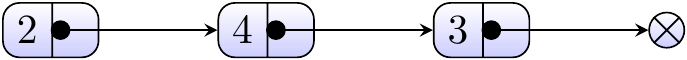
\includegraphics[width=0.9\linewidth]{tech-interview_files/figure-latex/unnamed-chunk-43-1} \caption{Some caption.}\label{fig:unnamed-chunk-43}
\end{figure}

\begin{itemize}
\item
  \begin{figure}
  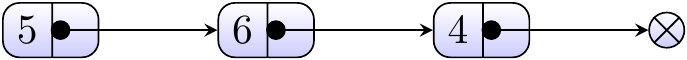
\includegraphics[width=0.9\linewidth]{tech-interview_files/figure-latex/unnamed-chunk-44-1} \caption{Some caption.}\label{fig:unnamed-chunk-44}
  \end{figure}
\end{itemize}

Output:

\begin{figure}
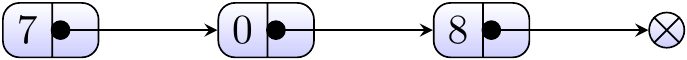
\includegraphics[width=0.9\linewidth]{tech-interview_files/figure-latex/unnamed-chunk-45-1} \caption{Some caption.}\label{fig:unnamed-chunk-45}
\end{figure}

Explanation: 342 + 465 = 807.

\hypertarget{solution-59}{%
\subsection{Solution}\label{solution-59}}

\hypertarget{walkthrough-100}{%
\subsubsection{Walkthrough\textbackslash{}}\label{walkthrough-100}}

First add two number digit by digit until one number run out of digit. Copy the other number for the remaining
of digits.

\hypertarget{analysis-107}{%
\subsubsection{Analysis\textbackslash{}}\label{analysis-107}}

Time complexity is O(n + m) as every node is visited once.

\hypertarget{algorithm-113}{%
\subsubsection{Algorithm\textbackslash{}}\label{algorithm-113}}

\hypertarget{java-code-66}{%
\subsection{Java Code}\label{java-code-66}}

\begin{Shaded}
\begin{Highlighting}[]
\KeywordTok{public}\NormalTok{ ListNode }\FunctionTok{addTwoNumbers}\NormalTok{(ListNode l1, ListNode l2) \{}
\NormalTok{    ListNode currentN1 = l1;}
\NormalTok{    ListNode currentN2 = l2;}
\NormalTok{    ListNode currentDigit = }\KeywordTok{new} \FunctionTok{ListNode}\NormalTok{(}\DecValTok{0}\NormalTok{);}
\NormalTok{    ListNode resultHead = currentDigit;}

    \DataTypeTok{int}\NormalTok{ digitCarry = }\DecValTok{0}\NormalTok{;}
    \DataTypeTok{int}\NormalTok{ digitSum = }\DecValTok{0}\NormalTok{;}

    \KeywordTok{while}\NormalTok{(currentN1 != }\KeywordTok{null}\NormalTok{ && currentN2 != }\KeywordTok{null}\NormalTok{) \{}
\NormalTok{        digitSum = currentN1.}\FunctionTok{val}\NormalTok{ + currentN2.}\FunctionTok{val}\NormalTok{ + digitCarry;}
\NormalTok{        digitCarry = digitSum / }\DecValTok{10}\NormalTok{;}
\NormalTok{        digitSum %= }\DecValTok{10}\NormalTok{;}

\NormalTok{        currentDigit.}\FunctionTok{next}\NormalTok{ = }\KeywordTok{new} \FunctionTok{ListNode}\NormalTok{(digitSum);}
\NormalTok{        currentDigit = currentDigit.}\FunctionTok{next}\NormalTok{;}

\NormalTok{        currentN1 = currentN1.}\FunctionTok{next}\NormalTok{;}
\NormalTok{        currentN2 = currentN2.}\FunctionTok{next}\NormalTok{;}
\NormalTok{    \}}

    \CommentTok{//Copy the remaining of number 1}
    \KeywordTok{while}\NormalTok{(currentN1 != }\KeywordTok{null}\NormalTok{) \{}
\NormalTok{        digitSum = currentN1.}\FunctionTok{val}\NormalTok{ + digitCarry;}
\NormalTok{        digitCarry = digitSum / }\DecValTok{10}\NormalTok{;}
\NormalTok{        digitSum %= }\DecValTok{10}\NormalTok{;}

\NormalTok{        currentDigit.}\FunctionTok{next}\NormalTok{ = }\KeywordTok{new} \FunctionTok{ListNode}\NormalTok{(digitSum);}
\NormalTok{        currentDigit = currentDigit.}\FunctionTok{next}\NormalTok{;}

\NormalTok{        currentN1 = currentN1.}\FunctionTok{next}\NormalTok{;}
\NormalTok{    \}}

    \CommentTok{//Copy the remaining of number 2}
    \KeywordTok{while}\NormalTok{(currentN2 != }\KeywordTok{null}\NormalTok{) \{}
\NormalTok{        digitSum = currentN2.}\FunctionTok{val}\NormalTok{ + digitCarry;}
\NormalTok{        digitCarry = digitSum / }\DecValTok{10}\NormalTok{;}
\NormalTok{        digitSum %= }\DecValTok{10}\NormalTok{;}

\NormalTok{        currentDigit.}\FunctionTok{next}\NormalTok{ = }\KeywordTok{new} \FunctionTok{ListNode}\NormalTok{(digitSum);}
\NormalTok{        currentDigit = currentDigit.}\FunctionTok{next}\NormalTok{;}

\NormalTok{        currentN2 = currentN2.}\FunctionTok{next}\NormalTok{;}
\NormalTok{    \}}

    \KeywordTok{if}\NormalTok{(digitCarry > }\DecValTok{0}\NormalTok{) \{}
\NormalTok{        currentDigit.}\FunctionTok{next}\NormalTok{ = }\KeywordTok{new} \FunctionTok{ListNode}\NormalTok{(digitCarry);}
\NormalTok{        currentDigit = currentDigit.}\FunctionTok{next}\NormalTok{;}
\NormalTok{    \}}

    \KeywordTok{return}\NormalTok{ resultHead.}\FunctionTok{next}\NormalTok{;}
\NormalTok{\}}
\end{Highlighting}
\end{Shaded}

\hypertarget{reverse-linked-list-leet-code-206-easy}{%
\section{Reverse Linked List / Leet Code 206 / Easy}\label{reverse-linked-list-leet-code-206-easy}}

\hypertarget{description-87}{%
\subsection{Description}\label{description-87}}

Reverse a singly linked list.

\hypertarget{example-83}{%
\subsection{Example}\label{example-83}}

Input:

\begin{figure}
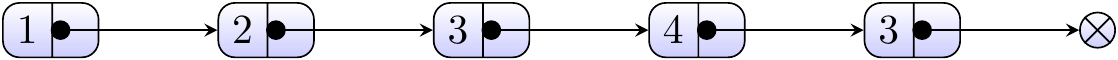
\includegraphics[width=0.9\linewidth]{tech-interview_files/figure-latex/unnamed-chunk-46-1} \caption{Some caption.}\label{fig:unnamed-chunk-46}
\end{figure}

Output:

\begin{figure}
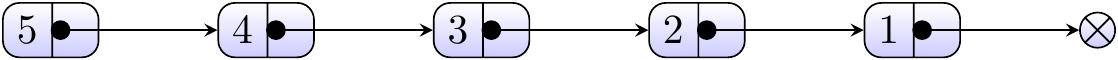
\includegraphics[width=0.9\linewidth]{tech-interview_files/figure-latex/unnamed-chunk-47-1} \caption{Some caption.}\label{fig:unnamed-chunk-47}
\end{figure}

\hypertarget{solution---recursive-5}{%
\subsection{Solution - Recursive}\label{solution---recursive-5}}

\hypertarget{walkthrough-101}{%
\subsubsection{Walkthrough\textbackslash{}}\label{walkthrough-101}}

For recursive solution, have a pointer remember original next and swap its link with the original head. Call
the method recursively.

\hypertarget{analysis-108}{%
\subsubsection{Analysis\textbackslash{}}\label{analysis-108}}

Time complexity is O(n) since every node is visited.

\hypertarget{algorithm-114}{%
\subsubsection{Algorithm\textbackslash{}}\label{algorithm-114}}

recursive \ref{recursive}

\hypertarget{java-code---recursive-5}{%
\subsection{Java Code - Recursive}\label{java-code---recursive-5}}

\begin{Shaded}
\begin{Highlighting}[]
\KeywordTok{public}\NormalTok{ ListNode }\FunctionTok{reverseList}\NormalTok{(ListNode node) \{}
    \KeywordTok{if}\NormalTok{(node == }\KeywordTok{null}\NormalTok{) \{}
        \KeywordTok{return} \KeywordTok{null}\NormalTok{;}
\NormalTok{    \} }\KeywordTok{else} \KeywordTok{if}\NormalTok{(node.}\FunctionTok{next}\NormalTok{ == }\KeywordTok{null}\NormalTok{) \{}
        \KeywordTok{return}\NormalTok{ node;}
\NormalTok{    \} }\KeywordTok{else}\NormalTok{ \{}
\NormalTok{        ListNode origNext = node.}\FunctionTok{next}\NormalTok{;}
\NormalTok{        ListNode newNode = }\FunctionTok{reverseList}\NormalTok{(origNext);}
        \CommentTok{//origNext -> node}
\NormalTok{        origNode.}\FunctionTok{next}\NormalTok{ = node;}
        \CommentTok{//delete link}
\NormalTok{        node.}\FunctionTok{next}\NormalTok{ = }\KeywordTok{null}\NormalTok{;}
        \KeywordTok{return}\NormalTok{ newNode;}
\NormalTok{    \}}
\NormalTok{\}}
\end{Highlighting}
\end{Shaded}

\hypertarget{solution---iterative}{%
\subsection{Solution - Iterative}\label{solution---iterative}}

\hypertarget{walkthrough-102}{%
\subsubsection{Walkthrough\textbackslash{}}\label{walkthrough-102}}

For iterative solution, have a helper pointer to remember the previous position and reverse the links between
current and headPrev nodes while iterating the list.

\begin{figure}
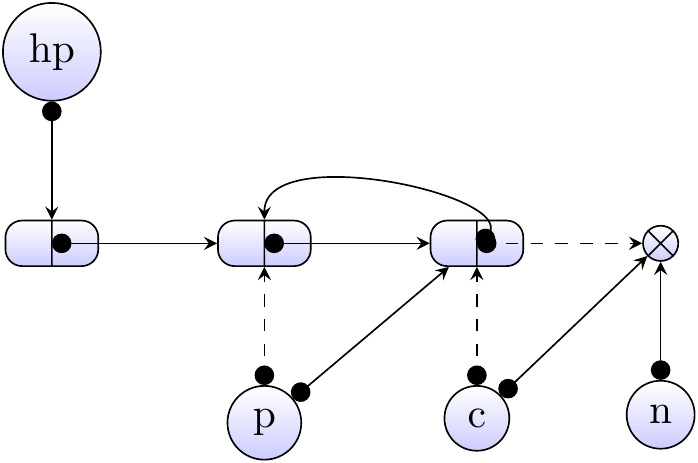
\includegraphics[width=0.9\linewidth]{tech-interview_files/figure-latex/unnamed-chunk-48-1} \caption{Some caption.}\label{fig:unnamed-chunk-48}
\end{figure}

Finally, reset where begin.next points to head of the list after reverse - tail of the original list, and return the
head of the reversed list.

\begin{figure}
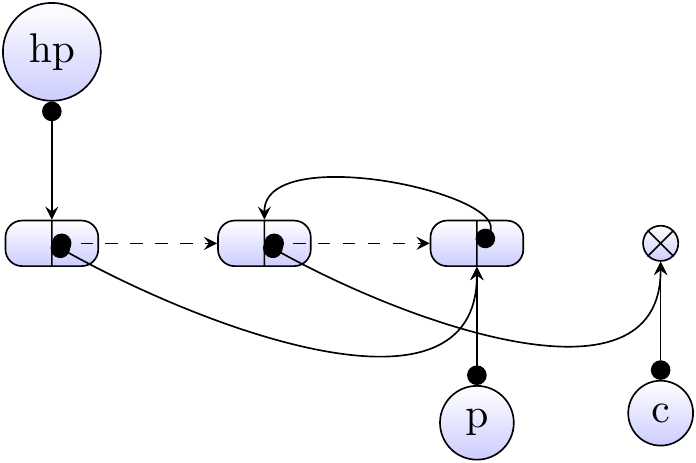
\includegraphics[width=0.9\linewidth]{tech-interview_files/figure-latex/unnamed-chunk-49-1} \caption{Some caption.}\label{fig:unnamed-chunk-49}
\end{figure}

\hypertarget{analysis-109}{%
\subsubsection{Analysis\textbackslash{}}\label{analysis-109}}

Time complexity is O(n) since every node is visited.

\hypertarget{algorithm-115}{%
\subsubsection{Algorithm\textbackslash{}}\label{algorithm-115}}

\hypertarget{java-code---iterative}{%
\subsection{Java Code - Iterative}\label{java-code---iterative}}

\begin{Shaded}
\begin{Highlighting}[]
\KeywordTok{public}\NormalTok{ ListNode }\FunctionTok{reverseList}\NormalTok{(ListNode head) \{}
    \KeywordTok{if}\NormalTok{(head == }\KeywordTok{null}\NormalTok{ || head.}\FunctionTok{next}\NormalTok{ == }\KeywordTok{null}\NormalTok{) \{}
        \KeywordTok{return}\NormalTok{ head;}
\NormalTok{    \}}

\NormalTok{    ListNode headPrev = }\KeywordTok{new} \FunctionTok{ListNode}\NormalTok{(}\DecValTok{0}\NormalTok{);}
\NormalTok{    headPrev.}\FunctionTok{next}\NormalTok{ = head;}

    \KeywordTok{return} \FunctionTok{reverse}\NormalTok{(headPrev);}
\NormalTok{\}}

\KeywordTok{public}\NormalTok{ ListNode }\FunctionTok{reverse}\NormalTok{(ListNode begin) \{}
\NormalTok{    ListNode prev = begin.}\FunctionTok{next}\NormalTok{;}
\NormalTok{    ListNode current = prev.}\FunctionTok{next}\NormalTok{;}

    \CommentTok{//reverse links between current and prev}
    \KeywordTok{while}\NormalTok{ (current != }\KeywordTok{null}\NormalTok{) \{}
\NormalTok{        ListNode next = current.}\FunctionTok{next}\NormalTok{;}
        \CommentTok{/*}
\CommentTok{        * swap links between current and prev}
\CommentTok{        */}
\NormalTok{        current.}\FunctionTok{next}\NormalTok{ = prev;}
\NormalTok{        prev = current;}
\NormalTok{        current = next;}
\NormalTok{    \}}

\NormalTok{    begin.}\FunctionTok{next}\NormalTok{.}\FunctionTok{next}\NormalTok{ = current;}
\NormalTok{    begin.}\FunctionTok{next}\NormalTok{ = prev;}

    \KeywordTok{return}\NormalTok{ begin.}\FunctionTok{next}\NormalTok{;}
\NormalTok{\}}
\end{Highlighting}
\end{Shaded}

\hypertarget{reverse-linked-list-ii-leet-code-92-medium}{%
\section{Reverse Linked List II / Leet Code 92 / Medium}\label{reverse-linked-list-ii-leet-code-92-medium}}

\hypertarget{description-88}{%
\subsection{Description}\label{description-88}}

Reverse a linked list from position m to n. Do it in one-pass

\hypertarget{example-84}{%
\subsection{Example}\label{example-84}}

Input:

\begin{figure}
\includegraphics[width=0.9\linewidth]{tech-interview_files/figure-latex/unnamed-chunk-50-1} \caption{Some caption.}\label{fig:unnamed-chunk-50}
\end{figure}

, m = 2, n = 4

Output:

\begin{figure}
\includegraphics[width=0.9\linewidth]{tech-interview_files/figure-latex/unnamed-chunk-51-1} \caption{Some caption.}\label{fig:unnamed-chunk-51}
\end{figure}

\hypertarget{solution-60}{%
\subsection{Solution}\label{solution-60}}

\hypertarget{walkthrough-103}{%
\subsubsection{Walkthrough\textbackslash{}}\label{walkthrough-103}}

Have a helper pointer to to move to (M-1) position and reverse the links between current and prev nodes while
iterating the list for (N-M) nodes.

\begin{figure}
\includegraphics[width=0.9\linewidth]{tech-interview_files/figure-latex/unnamed-chunk-52-1} \caption{Some caption.}\label{fig:unnamed-chunk-52}
\end{figure}

Finally, reset where begin.next points to head of the list after reverse - tail of the original list, and return the
tail of the reversed list.

\begin{figure}
\includegraphics[width=0.9\linewidth]{tech-interview_files/figure-latex/unnamed-chunk-53-1} \caption{Some caption.}\label{fig:unnamed-chunk-53}
\end{figure}

\hypertarget{analysis-110}{%
\subsubsection{Analysis\textbackslash{}}\label{analysis-110}}

Time complexity is O(n) as every node is visited once.

\hypertarget{algorithm-116}{%
\subsubsection{Algorithm\textbackslash{}}\label{algorithm-116}}

\hypertarget{java-code-67}{%
\subsection{Java Code}\label{java-code-67}}

\begin{Shaded}
\begin{Highlighting}[]
\KeywordTok{public}\NormalTok{ ListNode }\FunctionTok{reverseBetween}\NormalTok{(ListNode head, }\DataTypeTok{int}\NormalTok{ m, }\DataTypeTok{int}\NormalTok{ n) \{}
    \KeywordTok{if}\NormalTok{(head == }\KeywordTok{null}\NormalTok{) \{}
        \KeywordTok{return}\NormalTok{ head;}
\NormalTok{    \}}

    \CommentTok{//headHelper.next is original head}
\NormalTok{    ListNode headPrev = }\KeywordTok{new} \FunctionTok{ListNode}\NormalTok{(}\DecValTok{0}\NormalTok{);}
\NormalTok{    headPrev.}\FunctionTok{next}\NormalTok{ = head;}

\NormalTok{    ListNode mMinus1 = headPrev;}
    \CommentTok{//move to starting position}
    \KeywordTok{for}\NormalTok{ (}\DataTypeTok{int}\NormalTok{ i = }\DecValTok{0}\NormalTok{; i < m - }\DecValTok{1}\NormalTok{; i++) \{}
\NormalTok{        mMinus1 = mMinus1.}\FunctionTok{next}\NormalTok{;}
\NormalTok{    \}}

    \CommentTok{//reverse node between (m, n)}
    \FunctionTok{reverseList}\NormalTok{(mMinus1, n-m);}

    \KeywordTok{return}\NormalTok{ headPrev.}\FunctionTok{next}\NormalTok{;}
\NormalTok{\}}

\KeywordTok{public}\NormalTok{ ListNode }\FunctionTok{reverseList}\NormalTok{(ListNode begin, }\DataTypeTok{int}\NormalTok{ length) \{}
\NormalTok{    ListNode prev = begin.}\FunctionTok{next}\NormalTok{;}
\NormalTok{    ListNode current = prev.}\FunctionTok{next}\NormalTok{;}

    \CommentTok{//reverse links between current and prev}
    \DataTypeTok{int}\NormalTok{ i = }\DecValTok{0}\NormalTok{;}
    \KeywordTok{while}\NormalTok{ (i < length) \{}
\NormalTok{        ListNode next = current.}\FunctionTok{next}\NormalTok{;}
        \CommentTok{/*}
\CommentTok{        * swap links between current and prev}
\CommentTok{        */}
\NormalTok{        current.}\FunctionTok{next}\NormalTok{ = prev;}
\NormalTok{        prev = current;}
\NormalTok{        current = next;}
\NormalTok{        i++;}
\NormalTok{    \}}

    \CommentTok{// tail of reversed is head of original list}
\NormalTok{    ListNode tail = begin.}\FunctionTok{next}\NormalTok{;}

\NormalTok{    begin.}\FunctionTok{next}\NormalTok{.}\FunctionTok{next}\NormalTok{ = current;}
\NormalTok{    begin.}\FunctionTok{next}\NormalTok{ = prev;}

    \KeywordTok{return}\NormalTok{ tail;}
\NormalTok{\}}
\end{Highlighting}
\end{Shaded}

\hypertarget{reverse-nodes-in-k-group-leetcode-25-hard}{%
\section{Reverse Nodes in k-Group / LeetCode 25 / Hard}\label{reverse-nodes-in-k-group-leetcode-25-hard}}

\hypertarget{description-89}{%
\subsection{Description}\label{description-89}}

Given a linked list, reverse the nodes of a linked list k at a time and return its modified list. If the number of
nodes is not a multiple of k then left-out nodes in the end should remain as it is. You may not alter the values in
the nodes, only nodes itself may be changed.

\hypertarget{example-85}{%
\subsection{Example}\label{example-85}}

Input:

\begin{figure}
\includegraphics[width=0.9\linewidth]{tech-interview_files/figure-latex/unnamed-chunk-54-1} \caption{Some caption.}\label{fig:unnamed-chunk-54}
\end{figure}

k = 2 becomes

\begin{figure}
\includegraphics[width=0.9\linewidth]{tech-interview_files/figure-latex/unnamed-chunk-55-1} \caption{Some caption.}\label{fig:unnamed-chunk-55}
\end{figure}

k=3 becomes

\begin{figure}
\includegraphics[width=0.9\linewidth]{tech-interview_files/figure-latex/unnamed-chunk-56-1} \caption{Some caption.}\label{fig:unnamed-chunk-56}
\end{figure}

\hypertarget{solution-61}{%
\subsection{Solution}\label{solution-61}}

\hypertarget{walkthrough-104}{%
\subsubsection{Walkthrough\textbackslash{}}\label{walkthrough-104}}

Have a index to remember when to start reversing and when to stop and reverse the links between current and prev nodes
while iterating the list until the stop position is met.

\begin{figure}
\includegraphics[width=0.9\linewidth]{tech-interview_files/figure-latex/unnamed-chunk-57-1} \caption{Some caption.}\label{fig:unnamed-chunk-57}
\end{figure}

Finally, reset where begin.next points to head of the list after reverse - tail of the original list, and return the
tail of the reversed list.

\begin{figure}
\includegraphics[width=0.9\linewidth]{tech-interview_files/figure-latex/unnamed-chunk-58-1} \caption{Some caption.}\label{fig:unnamed-chunk-58}
\end{figure}

\hypertarget{analysis-111}{%
\subsubsection{Analysis\textbackslash{}}\label{analysis-111}}

Time complexity is O(n) as every node is visited once.

\hypertarget{algorithm-117}{%
\subsubsection{Algorithm\textbackslash{}}\label{algorithm-117}}

\hypertarget{java-code-68}{%
\subsection{Java Code}\label{java-code-68}}

\begin{Shaded}
\begin{Highlighting}[]
\KeywordTok{public}\NormalTok{ ListNode }\FunctionTok{reverseKGroup}\NormalTok{(ListNode head, }\DataTypeTok{int}\NormalTok{ k) \{}
    \KeywordTok{if}\NormalTok{(head==}\KeywordTok{null}\NormalTok{ || k==}\DecValTok{1}\NormalTok{) \{}
        \KeywordTok{return}\NormalTok{ head;}
\NormalTok{    \}}

\NormalTok{    ListNode headPrev = }\KeywordTok{new} \FunctionTok{ListNode}\NormalTok{(}\DecValTok{0}\NormalTok{);}
\NormalTok{    headPrev.}\FunctionTok{next}\NormalTok{ = head;}
\NormalTok{    ListNode prev = headPrev;}
    \DataTypeTok{int}\NormalTok{ i = }\DecValTok{0}\NormalTok{;}

\NormalTok{    ListNode current = head;}
    \KeywordTok{while}\NormalTok{(current!=}\KeywordTok{null}\NormalTok{)\{}
\NormalTok{        i++;}
        \KeywordTok{if}\NormalTok{((i % k) == }\DecValTok{0}\NormalTok{)\{}
\NormalTok{            ListNode revTail = }\FunctionTok{reverseList}\NormalTok{(prev, current.}\FunctionTok{next}\NormalTok{);}
\NormalTok{            prev = revTail;}
\NormalTok{            current = revTail.}\FunctionTok{next}\NormalTok{;}
\NormalTok{        \}}\KeywordTok{else}\NormalTok{\{}
\NormalTok{            current = current.}\FunctionTok{next}\NormalTok{;}
\NormalTok{        \}}
\NormalTok{    \}}

    \KeywordTok{return}\NormalTok{ headPrev.}\FunctionTok{next}\NormalTok{;}
\NormalTok{\}}


\KeywordTok{public}\NormalTok{ ListNode }\FunctionTok{reverseList}\NormalTok{(ListNode begin, ListNode end) \{}
\NormalTok{    ListNode prev = begin.}\FunctionTok{next}\NormalTok{;}
\NormalTok{    ListNode current = prev.}\FunctionTok{next}\NormalTok{;}

    \CommentTok{//reverse links between current and prev}
    \KeywordTok{while}\NormalTok{ (current != end) \{}
\NormalTok{        ListNode next = current.}\FunctionTok{next}\NormalTok{;}
        \CommentTok{/*}
\CommentTok{        * swap links between current and prev}
\CommentTok{        */}
\NormalTok{        current.}\FunctionTok{next}\NormalTok{ = prev;}
\NormalTok{        prev = current;}
\NormalTok{        current = next;}
\NormalTok{    \}}

    \CommentTok{// tail of reversed is head of original list}
\NormalTok{    ListNode tail = begin.}\FunctionTok{next}\NormalTok{;}

\NormalTok{    begin.}\FunctionTok{next}\NormalTok{.}\FunctionTok{next}\NormalTok{ = end;}
\NormalTok{    begin.}\FunctionTok{next}\NormalTok{ = prev;}

    \KeywordTok{return}\NormalTok{ tail;}
\NormalTok{\}}
\end{Highlighting}
\end{Shaded}

\hypertarget{linked-list-cycle-leet-code-141-easy}{%
\section{Linked List Cycle / Leet Code 141 / Easy}\label{linked-list-cycle-leet-code-141-easy}}

\hypertarget{description-90}{%
\subsection{Description}\label{description-90}}

Given a linked list, determine if it has a cycle in it.

To represent a cycle in the given linked list, we use an integer pos which represents the position
(0-indexed) in the linked list where tail connects to. If pos is -1, then there is no cycle in the linked
list.

\hypertarget{example-86}{%
\subsection{Example}\label{example-86}}

Input:

\begin{figure}
\includegraphics[width=0.9\linewidth]{tech-interview_files/figure-latex/unnamed-chunk-59-1} \caption{Some caption.}\label{fig:unnamed-chunk-59}
\end{figure}

Output: true. Explanation: There is a cycle in the linked list, where
tail connects to the second node.

Input:

\begin{figure}
\includegraphics[width=0.9\linewidth]{tech-interview_files/figure-latex/unnamed-chunk-60-1} \caption{Some caption.}\label{fig:unnamed-chunk-60}
\end{figure}

Output: true. Explanation: There is a cycle in the linked list, where tail
connects to the first node.

Input:

\begin{figure}
\includegraphics[width=0.9\linewidth]{tech-interview_files/figure-latex/unnamed-chunk-61-1} \caption{Some caption.}\label{fig:unnamed-chunk-61}
\end{figure}

Output: false. Explanation: There is no cycle in the linked list.

\hypertarget{solution-62}{%
\subsection{Solution}\label{solution-62}}

\hypertarget{walkthrough-105}{%
\subsubsection{Walkthrough\textbackslash{}}\label{walkthrough-105}}

Having two pointers, one running twice as fast as the other(p1 = p1.next; p2 = p2.next.next). If there is a
cycle, eventually (p1 == p2) representing a node in the cycle. A better traversal algorithm would make p1 at
the middle of the cycled list whereas p2 at the tail of the cycled list.

\hypertarget{analysis-112}{%
\subsubsection{Analysis\textbackslash{}}\label{analysis-112}}

Time complexity is O(n) as every node is visited once.

\hypertarget{algorithm-118}{%
\subsubsection{Algorithm\textbackslash{}}\label{algorithm-118}}

\hypertarget{java-code-69}{%
\subsection{Java Code}\label{java-code-69}}

\begin{Shaded}
\begin{Highlighting}[]
\KeywordTok{public} \DataTypeTok{boolean} \FunctionTok{hasCycle}\NormalTok{(ListNode head) \{}
    \KeywordTok{if}\NormalTok{(head == }\KeywordTok{null}\NormalTok{) \{}
        \KeywordTok{return} \KeywordTok{false}\NormalTok{;}
\NormalTok{    \}}

\NormalTok{    ListNode fast = head, slow = head;}

    \KeywordTok{while}\NormalTok{(fast != }\KeywordTok{null}\NormalTok{ && fast.}\FunctionTok{next}\NormalTok{ != }\KeywordTok{null}\NormalTok{) \{}
\NormalTok{        fast = fast.}\FunctionTok{next}\NormalTok{.}\FunctionTok{next}\NormalTok{;}
\NormalTok{        slow = slow.}\FunctionTok{next}\NormalTok{;}

        \KeywordTok{if}\NormalTok{(fast == slow) \{}
            \KeywordTok{return} \KeywordTok{true}\NormalTok{;}
\NormalTok{        \}}
\NormalTok{    \}}

    \KeywordTok{return} \KeywordTok{false}\NormalTok{;}
\NormalTok{\}}
\end{Highlighting}
\end{Shaded}

\hypertarget{linked-list-cycle-ii-leet-code-142-medium}{%
\section{Linked List Cycle II / Leet Code 142 / Medium}\label{linked-list-cycle-ii-leet-code-142-medium}}

\hypertarget{description-91}{%
\subsection{Description}\label{description-91}}

Given a linked list, return the node where the cycle begins. If there is no cycle, return null.

To represent a cycle in the given linked list, we use an integer pos which represents the position
(0-indexed) in the linked list where tail connects to. If pos is -1, then there is no cycle in the linked
list.

Note: Do not modify the linked list.

\hypertarget{example-87}{%
\subsection{Example}\label{example-87}}

Input:

\begin{figure}
\includegraphics[width=0.9\linewidth]{tech-interview_files/figure-latex/unnamed-chunk-62-1} \caption{Some caption.}\label{fig:unnamed-chunk-62}
\end{figure}

Output: tail connects to node index 1. Explanation: There is a cycle in the linked list, where tail
connects to the second node.

Input:

\begin{figure}
\includegraphics[width=0.9\linewidth]{tech-interview_files/figure-latex/unnamed-chunk-63-1} \caption{Some caption.}\label{fig:unnamed-chunk-63}
\end{figure}

Output: tail connects to node index 0. Explanation: There is a cycle in the linked list, where tail
connects to the first node.

Input:

\begin{figure}
\includegraphics[width=0.9\linewidth]{tech-interview_files/figure-latex/unnamed-chunk-64-1} \caption{Some caption.}\label{fig:unnamed-chunk-64}
\end{figure}

Output: null (no cycle). Explanation: There is no cycle in the linked list.

\hypertarget{solution-63}{%
\subsection{Solution}\label{solution-63}}

\hypertarget{walkthrough-106}{%
\subsubsection{Walkthrough\textbackslash{}}\label{walkthrough-106}}

Having two pointers, one talks twice as fast as the other. If there is a cycle (p1 == p2), p1 would be at
the middle of the cycled list whereas p2 at the tail of the cycled list. In other words, \emph{\# of steps
taken from header to p1 equals to \# of steps taken from p1 to p2.}

\hypertarget{analysis-113}{%
\subsubsection{Analysis\textbackslash{}}\label{analysis-113}}

Time complexity is O(n) as every node is visited once.

\hypertarget{algorithm-119}{%
\subsubsection{Algorithm\textbackslash{}}\label{algorithm-119}}

\hypertarget{java-code-70}{%
\subsection{Java Code}\label{java-code-70}}

\begin{Shaded}
\begin{Highlighting}[]
\KeywordTok{public}\NormalTok{ ListNode }\FunctionTok{detectCycle}\NormalTok{(ListNode head) \{}
    \KeywordTok{if}\NormalTok{(head == }\KeywordTok{null}\NormalTok{ || head.}\FunctionTok{next}\NormalTok{ == }\KeywordTok{null}\NormalTok{) \{}
        \KeywordTok{return} \KeywordTok{null}\NormalTok{;}
\NormalTok{    \}}

\NormalTok{    ListNode fast = head, slow = head;}
    \KeywordTok{while}\NormalTok{(fast != }\KeywordTok{null}\NormalTok{ && fast.}\FunctionTok{next}\NormalTok{ != }\KeywordTok{null}\NormalTok{) \{}
\NormalTok{        fast = fast.}\FunctionTok{next}\NormalTok{.}\FunctionTok{next}\NormalTok{;}
\NormalTok{        slow = slow.}\FunctionTok{next}\NormalTok{;}

        \KeywordTok{if}\NormalTok{(fast == slow) \{}
            \KeywordTok{break}\NormalTok{;}
\NormalTok{        \}}
\NormalTok{    \}}

    \KeywordTok{if}\NormalTok{(fast == slow) \{}
\NormalTok{        ListNode cycleHead = head;}
        \CommentTok{/*}
\CommentTok{         * slow is at middle of CYCLED list}
\CommentTok{         * Initially, cycleHead is at header}
\CommentTok{         * cycleHead --> slow == slow --> fast}
\CommentTok{         */}
        \KeywordTok{while}\NormalTok{(fast != cycleHead) \{}
\NormalTok{            fast = fast.}\FunctionTok{next}\NormalTok{;}
\NormalTok{            cycleHead = cycleHead.}\FunctionTok{next}\NormalTok{;}
\NormalTok{        \}}

        \KeywordTok{return}\NormalTok{ cycleHead;}
\NormalTok{    \} }\KeywordTok{else}\NormalTok{ \{}\CommentTok{//no cycle}
        \KeywordTok{return} \KeywordTok{null}\NormalTok{;}
\NormalTok{    \}}
\NormalTok{\}}
\end{Highlighting}
\end{Shaded}

\hypertarget{odd-even-linked-list-leet-code-328-medium}{%
\section{Odd Even Linked List / Leet Code 328 / Medium}\label{odd-even-linked-list-leet-code-328-medium}}

\hypertarget{description-92}{%
\subsection{Description}\label{description-92}}

Given a singly linked list, group all odd nodes together followed by the even nodes. Please note here we
are talking about the node number and not the value in the nodes.
You should try to do it in place.

\hypertarget{example-88}{%
\subsection{Example}\label{example-88}}

Input:

\begin{figure}
\includegraphics[width=0.9\linewidth]{tech-interview_files/figure-latex/unnamed-chunk-65-1} \caption{Some caption.}\label{fig:unnamed-chunk-65}
\end{figure}

Output:

\begin{figure}
\includegraphics[width=0.9\linewidth]{tech-interview_files/figure-latex/unnamed-chunk-66-1} \caption{Some caption.}\label{fig:unnamed-chunk-66}
\end{figure}

\hypertarget{solution-64}{%
\subsection{Solution}\label{solution-64}}

\hypertarget{walkthrough-107}{%
\subsubsection{Walkthrough\textbackslash{}}\label{walkthrough-107}}

Have two helper pointers to construct to list: one for odd nodes and one for even nodes. Assign those nodes
accordingly while traversing the list. Finally, connect odd nodes list to even nodes list.

\hypertarget{analysis-114}{%
\subsubsection{Analysis\textbackslash{}}\label{analysis-114}}

The program should run in O(1) Auxiliary Space and O(n) time complexity.

\hypertarget{algorithm-120}{%
\subsubsection{Algorithm\textbackslash{}}\label{algorithm-120}}

\hypertarget{java-code-71}{%
\subsection{Java Code}\label{java-code-71}}

\begin{Shaded}
\begin{Highlighting}[]
\KeywordTok{public}\NormalTok{ ListNode }\FunctionTok{oddEvenList}\NormalTok{(ListNode head) \{}
    \KeywordTok{if}\NormalTok{(head == }\KeywordTok{null}\NormalTok{ || head.}\FunctionTok{next}\NormalTok{ == }\KeywordTok{null}\NormalTok{ || head.}\FunctionTok{next}\NormalTok{.}\FunctionTok{next}\NormalTok{ == }\KeywordTok{null}\NormalTok{ ) \{}
        \KeywordTok{return}\NormalTok{ head;}
\NormalTok{    \}}

\NormalTok{    ListNode oddHeadPrev = }\KeywordTok{new} \FunctionTok{ListNode}\NormalTok{(}\DecValTok{0}\NormalTok{), currentOdd = oddHeadPrev;}
\NormalTok{    ListNode evnHeadPrev = }\KeywordTok{new} \FunctionTok{ListNode}\NormalTok{(}\DecValTok{0}\NormalTok{), currentEvn = evnHeadPrev;}
\NormalTok{    ListNode current = head;}

    \DataTypeTok{int}\NormalTok{ index = }\DecValTok{1}\NormalTok{;}

    \KeywordTok{while}\NormalTok{(current != }\KeywordTok{null}\NormalTok{) \{}
        \CommentTok{// Same as index % 2 == 1}
        \KeywordTok{if}\NormalTok{( (index & }\DecValTok{1}\NormalTok{) > }\DecValTok{0}\NormalTok{ ) \{}
\NormalTok{            currentOdd.}\FunctionTok{next}\NormalTok{ = current;}
\NormalTok{            currentOdd = currentOdd.}\FunctionTok{next}\NormalTok{;}
\NormalTok{        \} }\KeywordTok{else}\NormalTok{ \{}
\NormalTok{            currentEvn.}\FunctionTok{next}\NormalTok{ = current;}
\NormalTok{            currentEvn = currentEvn.}\FunctionTok{next}\NormalTok{;}
\NormalTok{        \}}

\NormalTok{        index++;}
\NormalTok{        current = current.}\FunctionTok{next}\NormalTok{;}
\NormalTok{    \}}

    \CommentTok{//connect odd nodes list with even nodes list}
\NormalTok{    currentOdd.}\FunctionTok{next}\NormalTok{ = evnHeadPrev.}\FunctionTok{next}\NormalTok{;}

    \CommentTok{//connect event nodes to null}
\NormalTok{    currentEvn.}\FunctionTok{next}\NormalTok{ = }\KeywordTok{null}\NormalTok{;}

    \KeywordTok{return}\NormalTok{ oddHeadPrev.}\FunctionTok{next}\NormalTok{;}
\NormalTok{\}}
\end{Highlighting}
\end{Shaded}

\hypertarget{merge-two-sorted-lists-leet-code-21-easy}{%
\section{Merge Two Sorted Lists / Leet Code 21 / Easy}\label{merge-two-sorted-lists-leet-code-21-easy}}

\hypertarget{description-93}{%
\subsection{Description}\label{description-93}}

Merge two sorted linked lists and return it as a new list. The new list should be made by splicing
together the nodes of the first two lists.

\hypertarget{example-89}{%
\subsection{Example}\label{example-89}}

\hypertarget{solution-65}{%
\subsection{Solution}\label{solution-65}}

\hypertarget{walkthrough-108}{%
\subsubsection{Walkthrough\textbackslash{}}\label{walkthrough-108}}

This is the same as merge() to sort a list in Leet Code 148. First we will create a new ListNode and a
current pointer. While traversing the node, compre the nodes at each list and nodes with smaller value
will attach to the final sorted list. Exit traversal when either list hits the end. If there are nodes
remained in either list, connect to that remaining nodes of the list.

\hypertarget{analysis-115}{%
\subsubsection{Analysis\textbackslash{}}\label{analysis-115}}

The cost for each merge is O(n) as every node is visited once in the list. There are two lists, thus the overall time
complexity remains O(n).

\hypertarget{algorithm-121}{%
\subsubsection{Algorithm\textbackslash{}}\label{algorithm-121}}

\hypertarget{java-code-72}{%
\subsection{Java Code}\label{java-code-72}}

\begin{Shaded}
\begin{Highlighting}[]
\KeywordTok{public}\NormalTok{ ListNode }\FunctionTok{mergeTwoLists}\NormalTok{(ListNode l1, ListNode l2) \{}
\NormalTok{    ListNode headPrev = }\KeywordTok{new} \FunctionTok{ListNode}\NormalTok{(}\DecValTok{0}\NormalTok{), current = headPrev;}

    \KeywordTok{while}\NormalTok{(l1 != }\KeywordTok{null}\NormalTok{ && l2 != }\KeywordTok{null}\NormalTok{) \{}
        \KeywordTok{if}\NormalTok{(l1.}\FunctionTok{val}\NormalTok{ < l2.}\FunctionTok{val}\NormalTok{) \{}
            \CommentTok{//l1 < l2}
\NormalTok{            current.}\FunctionTok{next}\NormalTok{ = l1;}
\NormalTok{            l1 = l1.}\FunctionTok{next}\NormalTok{;}
\NormalTok{        \} }\KeywordTok{else}\NormalTok{ \{}
\NormalTok{            current.}\FunctionTok{next}\NormalTok{ = l2;}
\NormalTok{            l2 = l2.}\FunctionTok{next}\NormalTok{;}
\NormalTok{        \}}
\NormalTok{        current = current.}\FunctionTok{next}\NormalTok{;}
\NormalTok{    \}}

    \CommentTok{// connect to the rest of the remaining nodes}
    \KeywordTok{if}\NormalTok{(l1 != }\KeywordTok{null}\NormalTok{) \{}
\NormalTok{        current.}\FunctionTok{next}\NormalTok{ = l1;}
\NormalTok{    \} }\KeywordTok{else}\NormalTok{ \{}
        \CommentTok{// l2 = remaining of list or null}
\NormalTok{        current.}\FunctionTok{next}\NormalTok{ = l2;}
\NormalTok{    \}}

    \KeywordTok{return}\NormalTok{ headPrev.}\FunctionTok{next}\NormalTok{;}
\NormalTok{\}}
\end{Highlighting}
\end{Shaded}

\hypertarget{merge-k-sorted-lists-leet-code-23-hard}{%
\section{Merge k Sorted Lists / Leet Code 23 / Hard}\label{merge-k-sorted-lists-leet-code-23-hard}}

\hypertarget{description-94}{%
\subsection{Description}\label{description-94}}

Merge k sorted linked lists and return it as one sorted list. Analyze and describe its complexity.

\hypertarget{example-90}{%
\subsection{Example}\label{example-90}}

\hypertarget{solution---merge-lists-one-by-one}{%
\subsection{Solution - Merge lists one by one}\label{solution---merge-lists-one-by-one}}

\hypertarget{walkthrough-109}{%
\subsubsection{Walkthrough\textbackslash{}}\label{walkthrough-109}}

One solution is to leverage the previous problem of merging 2 list.

\hypertarget{analysis-116}{%
\subsubsection{Analysis\textbackslash{}}\label{analysis-116}}

We will need to merge two lists for (k-1) times, where each
merge() will cost O(n) in time complexity and O(1) in Auxiliary Space. The total cost for merge is
\(\sum_{i=1}^{k-1} (i * \frac{n}{k} + \frac{n}{k}) = O(k \cdot n)\) in time complexity, where n is the
total node number in k list. and O(1) in Auxiliary Space. However, this would not be an efficient solution if k
is large.

\hypertarget{algorithm-122}{%
\subsubsection{Algorithm\textbackslash{}}\label{algorithm-122}}

\hypertarget{java-code---merge-lists-one-by-one}{%
\subsection{Java Code - Merge lists one by one}\label{java-code---merge-lists-one-by-one}}

\begin{Shaded}
\begin{Highlighting}[]
\KeywordTok{public}\NormalTok{ ListNode }\FunctionTok{mergeKLists}\NormalTok{(ListNode[] lists) \{}
    \KeywordTok{if}\NormalTok{(lists.}\FunctionTok{length}\NormalTok{ == }\DecValTok{0}\NormalTok{) \{}
        \KeywordTok{return} \KeywordTok{null}\NormalTok{;}
\NormalTok{    \}}

\NormalTok{    ListNode newHead = lists[}\DecValTok{0}\NormalTok{];}

    \CommentTok{//merge k-1 times}
    \KeywordTok{for}\NormalTok{(}\DataTypeTok{int}\NormalTok{ i = }\DecValTok{1}\NormalTok{; i < lists.}\FunctionTok{length}\NormalTok{; i++) \{}
\NormalTok{        newHead = }\FunctionTok{merge}\NormalTok{(newHead, lists[i]);}
\NormalTok{    \}}

    \KeywordTok{return}\NormalTok{ newHead;}
\NormalTok{\}}

\KeywordTok{public}\NormalTok{ ListNode }\FunctionTok{merge}\NormalTok{(ListNode l1, ListNode l2) \{}
\NormalTok{    ListNode headPrev = }\KeywordTok{new} \FunctionTok{ListNode}\NormalTok{(}\DecValTok{0}\NormalTok{), current = headPrev;}

    \KeywordTok{while}\NormalTok{(l1 != }\KeywordTok{null}\NormalTok{ && l2 != }\KeywordTok{null}\NormalTok{) \{}
        \KeywordTok{if}\NormalTok{(l1.}\FunctionTok{val}\NormalTok{ < l2.}\FunctionTok{val}\NormalTok{) \{}
            \CommentTok{//l1 < l2}
\NormalTok{            current.}\FunctionTok{next}\NormalTok{ = l1;}
\NormalTok{            l1 = l1.}\FunctionTok{next}\NormalTok{;}
\NormalTok{        \} }\KeywordTok{else}\NormalTok{ \{}
\NormalTok{            current.}\FunctionTok{next}\NormalTok{ = l2;}
\NormalTok{            l2 = l2.}\FunctionTok{next}\NormalTok{;}
\NormalTok{        \}}
\NormalTok{        current = current.}\FunctionTok{next}\NormalTok{;}
\NormalTok{    \}}

    \CommentTok{// connect to the rest of the remaining nodes}
    \KeywordTok{if}\NormalTok{(l1 != }\KeywordTok{null}\NormalTok{) \{}
\NormalTok{        current.}\FunctionTok{next}\NormalTok{ = l1;}
\NormalTok{    \} }\KeywordTok{else}\NormalTok{ \{}
\NormalTok{        current.}\FunctionTok{next}\NormalTok{ = l2;}
\NormalTok{    \}}

    \KeywordTok{return}\NormalTok{ headPrev.}\FunctionTok{next}\NormalTok{;}
\NormalTok{\}}
\end{Highlighting}
\end{Shaded}

\hypertarget{solution---min-heap}{%
\subsection{Solution - Min Heap}\label{solution---min-heap}}

\hypertarget{walkthrough-110}{%
\subsubsection{Walkthrough\textbackslash{}}\label{walkthrough-110}}

We could compare every leading elements in k lists and retrieve the node with the smallest value using Min Heap.

\hypertarget{analysis-117}{%
\subsubsection{Analysis\textbackslash{}}\label{analysis-117}}

Since the original k lists were sorted, therefore, we could retrieve all \(n \cdot k\) elements in
sorted order by retrieve the min element from PriorityQueue (min heap). The comparison cost is O(log k) for every pop
and insertion to the priority queue since there are at most k elements (from k list). Additionally, there are
a total number of n nodes in all lists. Thus, the overall time complexity is \(O(\log k \cdot n)\) and Auxiliary Space
for the final list is O(n), where n is the total node number in all k lists.

\hypertarget{algorithm-123}{%
\subsubsection{Algorithm\textbackslash{}}\label{algorithm-123}}

bfs \ref{bfs}, heap \ref{heap}

\hypertarget{java-code---min-heap}{%
\subsection{Java Code - Min Heap}\label{java-code---min-heap}}

\begin{Shaded}
\begin{Highlighting}[]
\KeywordTok{public}\NormalTok{ ListNode }\FunctionTok{mergeKLists}\NormalTok{(ListNode[] lists) \{}
    \KeywordTok{if}\NormalTok{(lists.}\FunctionTok{length}\NormalTok{ == }\DecValTok{0}\NormalTok{) \{}
        \KeywordTok{return} \KeywordTok{null}\NormalTok{;}
\NormalTok{    \}}

\NormalTok{    ListNode head = }\KeywordTok{null}\NormalTok{, current = }\KeywordTok{null}\NormalTok{;}

    \BuiltInTok{PriorityQueue}\NormalTok{<ListNode> queue = }\KeywordTok{new} \BuiltInTok{PriorityQueue}\NormalTok{<>(}\KeywordTok{new} \BuiltInTok{Comparator}\NormalTok{<ListNode>() \{}
        \AttributeTok{@Override}
        \KeywordTok{public} \DataTypeTok{int} \FunctionTok{compare}\NormalTok{(ListNode node1, ListNode node2) \{}
            \KeywordTok{return}\NormalTok{ node1.}\FunctionTok{val}\NormalTok{ - node2.}\FunctionTok{val}\NormalTok{;}
\NormalTok{        \}}
\NormalTok{    \});}

    \CommentTok{//insert all heads into the priority queue}
    \KeywordTok{for}\NormalTok{(ListNode headOfList : lists) \{}
        \KeywordTok{if}\NormalTok{(headOfList != }\KeywordTok{null}\NormalTok{) \{}
\NormalTok{            queue.}\FunctionTok{offer}\NormalTok{(headOfList);}
\NormalTok{        \}}
\NormalTok{    \}}


    \KeywordTok{while}\NormalTok{(!queue.}\FunctionTok{isEmpty}\NormalTok{()) \{}
\NormalTok{        ListNode node = queue.}\FunctionTok{poll}\NormalTok{();}

        \CommentTok{//add next node into priority queue}
        \KeywordTok{if}\NormalTok{(node.}\FunctionTok{next}\NormalTok{ != }\KeywordTok{null}\NormalTok{) \{}
\NormalTok{            queue.}\FunctionTok{offer}\NormalTok{(node.}\FunctionTok{next}\NormalTok{);}
\NormalTok{        \}}

        \CommentTok{// construct the list with the min element from queue}
        \KeywordTok{if}\NormalTok{(head == }\KeywordTok{null}\NormalTok{) \{}
\NormalTok{            head = node;}
\NormalTok{            current = node;}
\NormalTok{        \} }\KeywordTok{else}\NormalTok{ \{}
\NormalTok{            current.}\FunctionTok{next}\NormalTok{ = node;}
\NormalTok{            current = current.}\FunctionTok{next}\NormalTok{;}
\NormalTok{        \}}
\NormalTok{    \}}

    \KeywordTok{return}\NormalTok{ head;}
\NormalTok{\}}
\end{Highlighting}
\end{Shaded}

\hypertarget{palindrome-linked-list-leet-code-234-easy}{%
\section{Palindrome Linked List / Leet Code 234 / Easy}\label{palindrome-linked-list-leet-code-234-easy}}

\hypertarget{description-95}{%
\subsection{Description}\label{description-95}}

Given a singly linked list, determine if it is a palindrome.

\hypertarget{example-91}{%
\subsection{Example}\label{example-91}}

Input:

\begin{figure}
\includegraphics[width=0.9\linewidth]{tech-interview_files/figure-latex/unnamed-chunk-67-1} \caption{Some caption.}\label{fig:unnamed-chunk-67}
\end{figure}

return false

Output:

\begin{figure}
\includegraphics[width=0.9\linewidth]{tech-interview_files/figure-latex/unnamed-chunk-68-1} \caption{Some caption.}\label{fig:unnamed-chunk-68}
\end{figure}

return true

\hypertarget{solution-66}{%
\subsection{Solution}\label{solution-66}}

\hypertarget{walkthrough-111}{%
\subsubsection{Walkthrough\textbackslash{}}\label{walkthrough-111}}

Locate the mid node, and use that to reverse the 2nd half of the list. We will have two sublists: {[}o, \ldots{}, m{]} and
{[}r, \ldots{}, m{]}.

Event number of list:

\begin{figure}
\includegraphics[width=0.9\linewidth]{tech-interview_files/figure-latex/unnamed-chunk-69-1} \caption{Some caption.}\label{fig:unnamed-chunk-69}
\end{figure}

Odd number of list:

\begin{figure}
\includegraphics[width=0.9\linewidth]{tech-interview_files/figure-latex/unnamed-chunk-70-1} \caption{Some caption.}\label{fig:unnamed-chunk-70}
\end{figure}

Traverse the two sublists, beginning at head of original and head of reversed sublists respectively. If any node is
not equal, then it is NOT palindrome.

\hypertarget{analysis-118}{%
\subsubsection{Analysis\textbackslash{}}\label{analysis-118}}

Time complexity is O(n) as every node is visited once.

\hypertarget{algorithm-124}{%
\subsubsection{Algorithm\textbackslash{}}\label{algorithm-124}}

\hypertarget{java-code-73}{%
\subsection{Java Code}\label{java-code-73}}

\begin{Shaded}
\begin{Highlighting}[]
\KeywordTok{public} \DataTypeTok{boolean} \FunctionTok{isPalindrome}\NormalTok{(ListNode head) \{}
    \KeywordTok{if}\NormalTok{(head == }\KeywordTok{null}\NormalTok{ || head.}\FunctionTok{next}\NormalTok{ == }\KeywordTok{null}\NormalTok{) \{}
        \KeywordTok{return} \KeywordTok{true}\NormalTok{;}
\NormalTok{    \}}

\NormalTok{    ListNode mid = head, tail = head;}

    \CommentTok{//locating mid and tail nodes}
    \KeywordTok{while}\NormalTok{(tail.}\FunctionTok{next}\NormalTok{ != }\KeywordTok{null}\NormalTok{ && tail.}\FunctionTok{next}\NormalTok{.}\FunctionTok{next}\NormalTok{ != }\KeywordTok{null}\NormalTok{) \{}
\NormalTok{        mid = mid.}\FunctionTok{next}\NormalTok{;}
\NormalTok{        tail = tail.}\FunctionTok{next}\NormalTok{.}\FunctionTok{next}\NormalTok{;}
\NormalTok{    \}}

    \CommentTok{// retrieve the head of reversed 2nd half sublist}
\NormalTok{    ListNode reversed2ndHalfHead = }\FunctionTok{reverse}\NormalTok{(mid);}

\NormalTok{    ListNode currentOrg = head, currentRev = reversed2ndHalfHead;}

    \KeywordTok{while}\NormalTok{(currentOrg != }\KeywordTok{null}\NormalTok{ && currentRev != }\KeywordTok{null}\NormalTok{) \{}
        \CommentTok{//if any in original 1st half does not match reversed 2nd half}
        \KeywordTok{if}\NormalTok{(currentOrg.}\FunctionTok{val}\NormalTok{ != currentRev.}\FunctionTok{val}\NormalTok{) \{}
            \KeywordTok{return} \KeywordTok{false}\NormalTok{;}
\NormalTok{        \}}

\NormalTok{        currentOrg = currentOrg.}\FunctionTok{next}\NormalTok{;}
\NormalTok{        currentRev = currentRev.}\FunctionTok{next}\NormalTok{;}
\NormalTok{    \}}

    \KeywordTok{return} \KeywordTok{true}\NormalTok{;}
\NormalTok{\}}

\KeywordTok{public}\NormalTok{ ListNode }\FunctionTok{reverse}\NormalTok{(ListNode head) \{}
\NormalTok{    ListNode headPrev = }\KeywordTok{new} \FunctionTok{ListNode}\NormalTok{(}\DecValTok{0}\NormalTok{);}
\NormalTok{    ListNode current = head;}

    \CommentTok{//reverse links between current and prev}
    \KeywordTok{while}\NormalTok{ (current != }\KeywordTok{null}\NormalTok{) \{}
\NormalTok{        ListNode next = current.}\FunctionTok{next}\NormalTok{;}

        \CommentTok{/*}
\CommentTok{        * swap links between current and prev}
\CommentTok{        */}
\NormalTok{        current.}\FunctionTok{next}\NormalTok{ = headPrev.}\FunctionTok{next}\NormalTok{;}
\NormalTok{        headPrev.}\FunctionTok{next}\NormalTok{ = current;}
\NormalTok{        current = next;}
\NormalTok{    \}}

    \KeywordTok{return}\NormalTok{ headPrev.}\FunctionTok{next}\NormalTok{;}
\NormalTok{\}}
\end{Highlighting}
\end{Shaded}

\hypertarget{intersection-of-two-linked-lists-leet-code-160-easy}{%
\section{Intersection of Two Linked Lists / Leet Code 160 / Easy}\label{intersection-of-two-linked-lists-leet-code-160-easy}}

\hypertarget{description-96}{%
\subsection{Description}\label{description-96}}

Write a program to find the node at which the intersection of two singly linked lists begins.

\begin{verbatim}
*  If the two linked lists have no intersection at all, return null.
*  The linked lists must retain their original structure after the function returns.
*  You may assume there are no cycles anywhere in the entire linked structure.
*  Your code should preferably run in O(n) time and use only O(1) memory.
*  The intersected nodes must continue to the end of both lists.
*  If two nodes intersect, two node pointers refer to the same ListNode object in memory.
\end{verbatim}

\hypertarget{example-92}{%
\subsection{Example}\label{example-92}}

Input:

\begin{figure}
\includegraphics[width=0.9\linewidth]{tech-interview_files/figure-latex/unnamed-chunk-71-1} \caption{Some caption.}\label{fig:unnamed-chunk-71}
\end{figure}

Output: Reference of the node with value = 8
Input Explanation: The intersected node's value is 8 (note that this must not be 0 if the two lists
intersect). From the head of A, it reads as {[}4,1,8,4,5{]}. From the head of B, it reads as
{[}5,0,1,8,4,5{]}. There are 2 nodes before the intersected node in A; There are 3 nodes before the
intersected node in B.

\hypertarget{solution-67}{%
\subsection{Solution}\label{solution-67}}

\hypertarget{walkthrough-112}{%
\subsubsection{Walkthrough\textbackslash{}}\label{walkthrough-112}}

First we compute the length of both list and we get rid of the leading extra node of the longer list.
For the \# of remaining nodes of the longer list should equal to the \# of shorter list. We traverse
both list, and determine when (p1 == p2) - instead of (p1.val == p2.val)

\hypertarget{analysis-119}{%
\subsubsection{Analysis\textbackslash{}}\label{analysis-119}}

Time complexity is O(n) as every node is visited once.

\hypertarget{algorithm-125}{%
\subsubsection{Algorithm\textbackslash{}}\label{algorithm-125}}

\hypertarget{java-code-74}{%
\subsection{Java Code}\label{java-code-74}}

\begin{Shaded}
\begin{Highlighting}[]
\KeywordTok{public}\NormalTok{ ListNode }\FunctionTok{getIntersectionNode}\NormalTok{(ListNode headA, ListNode headB) \{}
    \DataTypeTok{int}\NormalTok{ lenA = }\DecValTok{0}\NormalTok{, lenB = }\DecValTok{0}\NormalTok{;}

    \CommentTok{//compute length of both lists}
    \KeywordTok{for}\NormalTok{(ListNode current = headA; current != }\KeywordTok{null}\NormalTok{; current = current.}\FunctionTok{next}\NormalTok{, lenA++);}
    \KeywordTok{for}\NormalTok{(ListNode current = headB; current != }\KeywordTok{null}\NormalTok{; current = current.}\FunctionTok{next}\NormalTok{, lenB++);}

    \CommentTok{//both conditions need to be the same}
\NormalTok{    ListNode currentLonger = lenA > lenB ? headA : headB;}
\NormalTok{    ListNode currentShorter = lenA > lenB ? headB : headA;}

    \CommentTok{//Move currentLonger to the position where remaining of nodes equal to len(currentShorter)}
    \KeywordTok{for}\NormalTok{(}\DataTypeTok{int}\NormalTok{ i = }\DecValTok{0}\NormalTok{; i < }\BuiltInTok{Math}\NormalTok{.}\FunctionTok{abs}\NormalTok{(lenA - lenB); i++, currentLonger = currentLonger.}\FunctionTok{next}\NormalTok{);}

    \KeywordTok{while}\NormalTok{(currentLonger != }\KeywordTok{null}\NormalTok{ && currentShorter != }\KeywordTok{null}\NormalTok{) \{}
        \CommentTok{//If the node intersect, nodeA == nodeB}
        \KeywordTok{if}\NormalTok{(currentLonger == currentShorter) \{}
            \CommentTok{//return current node}
            \KeywordTok{return}\NormalTok{ currentLonger;}
\NormalTok{        \}}

\NormalTok{        currentLonger = currentLonger.}\FunctionTok{next}\NormalTok{;}
\NormalTok{        currentShorter = currentShorter.}\FunctionTok{next}\NormalTok{;}
\NormalTok{    \}}

    \CommentTok{//no match}
    \KeywordTok{return} \KeywordTok{null}\NormalTok{;}
\NormalTok{\}}
\end{Highlighting}
\end{Shaded}

\hypertarget{remove-nth-node-from-end-of-list-leet-code-19-medium}{%
\section{Remove Nth Node From End of List / Leet Code 19 / Medium}\label{remove-nth-node-from-end-of-list-leet-code-19-medium}}

\hypertarget{description-97}{%
\subsection{Description}\label{description-97}}

Given a linked list, remove the n-th node from the end of list and return its head.

\hypertarget{example-93}{%
\subsection{Example}\label{example-93}}

Input:

\begin{figure}
\includegraphics[width=0.9\linewidth]{tech-interview_files/figure-latex/unnamed-chunk-72-1} \caption{Some caption.}\label{fig:unnamed-chunk-72}
\end{figure}

, and n = 2.

Output:

\begin{figure}
\includegraphics[width=0.9\linewidth]{tech-interview_files/figure-latex/unnamed-chunk-73-1} \caption{Some caption.}\label{fig:unnamed-chunk-73}
\end{figure}

\hypertarget{solution---two-pass}{%
\subsection{Solution - TWO Pass}\label{solution---two-pass}}

\hypertarget{walkthrough-113}{%
\subsubsection{Walkthrough\textbackslash{}}\label{walkthrough-113}}

The simpliest solution is to do solve this problem in two passes. First round is to find out the length of the list,
whileas the second iteration is to iterate to the node posiion \(length -n + 1\) or prev node position \(length - n\),
begining from a dummy node headPrev. Finally, we need to check and move the head node appropriately if we are deleting
it.

\hypertarget{analysis-120}{%
\subsubsection{Analysis\textbackslash{}}\label{analysis-120}}

Time complexity is O(n) as every node is visited once.

\hypertarget{algorithm-126}{%
\subsubsection{Algorithm\textbackslash{}}\label{algorithm-126}}

\hypertarget{java-code---two-pass}{%
\subsection{Java Code - TWO Pass}\label{java-code---two-pass}}

\begin{Shaded}
\begin{Highlighting}[]
\KeywordTok{public}\NormalTok{ ListNode }\FunctionTok{removeNthFromEnd}\NormalTok{(ListNode head, }\DataTypeTok{int}\NormalTok{ n) \{}
    \KeywordTok{if}\NormalTok{(head == }\KeywordTok{null}\NormalTok{) \{}
        \KeywordTok{return} \KeywordTok{null}\NormalTok{;}
\NormalTok{    \}}

    \CommentTok{//Quick check to see if we are deleting the only node in the list}
    \KeywordTok{if}\NormalTok{ (head.}\FunctionTok{next}\NormalTok{ == }\KeywordTok{null}\NormalTok{ && n <= }\DecValTok{1}\NormalTok{)\{}
        \KeywordTok{return} \KeywordTok{null}\NormalTok{;}
\NormalTok{    \}}

    \DataTypeTok{int}\NormalTok{ length = }\DecValTok{0}\NormalTok{;}

    \CommentTok{//1st pass: to get length of the list}
    \KeywordTok{for}\NormalTok{(ListNode current = head; current != }\KeywordTok{null}\NormalTok{; current = current.}\FunctionTok{next}\NormalTok{) \{}
\NormalTok{        length++;}
\NormalTok{    \}}

    \CommentTok{// removal position is over list length}
    \KeywordTok{if}\NormalTok{(n > length) \{}
        \KeywordTok{return}\NormalTok{ head;}
\NormalTok{    \}}

    \CommentTok{//move to the position before the target}
    \DataTypeTok{int}\NormalTok{ position = length - n;}

    \CommentTok{//keep track of current traversed # of nodes}
    \DataTypeTok{int}\NormalTok{ count = }\DecValTok{0}\NormalTok{;}

\NormalTok{    ListNode headPrev = }\KeywordTok{new} \FunctionTok{ListNode}\NormalTok{(}\DecValTok{0}\NormalTok{);}
\NormalTok{    headPrev.}\FunctionTok{next}\NormalTok{ = head;}
\NormalTok{    ListNode removedPrev = headPrev;}

    \CommentTok{//2nd pass: move to the one before target}
    \KeywordTok{while}\NormalTok{( count < position) \{}
\NormalTok{        removedPrev = removedPrev.}\FunctionTok{next}\NormalTok{;}
\NormalTok{        count++;}
\NormalTok{    \}}

\NormalTok{    removedPrev.}\FunctionTok{next}\NormalTok{ = removedPrev.}\FunctionTok{next}\NormalTok{.}\FunctionTok{next}\NormalTok{;}

    \CommentTok{//if removing head, renew head}
    \KeywordTok{if}\NormalTok{(removedPrev == headPrev) \{}
\NormalTok{        head = removedPrev.}\FunctionTok{next}\NormalTok{;}
\NormalTok{    \}}


    \KeywordTok{return}\NormalTok{ head;}
\NormalTok{\}}
\end{Highlighting}
\end{Shaded}

\hypertarget{solution---one-pass}{%
\subsection{Solution - ONE Pass}\label{solution---one-pass}}

\hypertarget{walkthrough-114}{%
\subsubsection{Walkthrough\textbackslash{}}\label{walkthrough-114}}

The simpliest solution is to do solve this problem in two passes. First round is to find out the length of the list,
whileas the second iteration is to iterate to the node posiion \(length -n + 1\) or prev node position \(length - n\),
begining from a dummy node headPrev. Finally, we need to check and move the head node appropriately if we are deleting
it.

\hypertarget{analysis-121}{%
\subsubsection{Analysis\textbackslash{}}\label{analysis-121}}

Time complexity is O(n) as every node is visited once.

\hypertarget{java-code---one-pass}{%
\subsection{Java Code - ONE Pass}\label{java-code---one-pass}}

\begin{Shaded}
\begin{Highlighting}[]
\KeywordTok{public}\NormalTok{ ListNode }\FunctionTok{removeNthFromEnd}\NormalTok{(ListNode head, }\DataTypeTok{int}\NormalTok{ n) \{}
    \CommentTok{//Quick check to see if we are deleting the only node in the list}
    \KeywordTok{if}\NormalTok{ (head.}\FunctionTok{next}\NormalTok{ == }\KeywordTok{null}\NormalTok{ && n == }\DecValTok{1}\NormalTok{)\{}
        \KeywordTok{return} \KeywordTok{null}\NormalTok{;}
\NormalTok{    \}}

    \CommentTok{//keep track of current traversed # of nodes}
    \DataTypeTok{int}\NormalTok{ count = }\DecValTok{0}\NormalTok{;}

    \CommentTok{//Add a node to the begining of our linked list to make deletions easier at the top}
\NormalTok{    ListNode headPrev = }\KeywordTok{new} \FunctionTok{ListNode}\NormalTok{(}\DecValTok{0}\NormalTok{);}
\NormalTok{    headPrev.}\FunctionTok{next}\NormalTok{ = head;}

\NormalTok{    ListNode current = headPrev;}
\NormalTok{    ListNode removedPrev = headPrev;}

    \KeywordTok{while}\NormalTok{(current != }\KeywordTok{null}\NormalTok{) \{}
\NormalTok{        count++;}

        \KeywordTok{if}\NormalTok{( (count - n) > }\DecValTok{1}\NormalTok{ ) \{}
\NormalTok{            removedPrev = removedPrev.}\FunctionTok{next}\NormalTok{;}
\NormalTok{        \}}

        \KeywordTok{if}\NormalTok{(current.}\FunctionTok{next}\NormalTok{ == }\KeywordTok{null}\NormalTok{) \{}
            \CommentTok{//the last node, removedPrev is also at the right position}

            \KeywordTok{if}\NormalTok{(removedPrev.}\FunctionTok{next}\NormalTok{ != }\KeywordTok{null}\NormalTok{ && removedPrev.}\FunctionTok{next}\NormalTok{.}\FunctionTok{next}\NormalTok{ == }\KeywordTok{null}\NormalTok{) \{}
                \CommentTok{//to remove tail node}
\NormalTok{                removedPrev.}\FunctionTok{next}\NormalTok{ = }\KeywordTok{null}\NormalTok{;}
\NormalTok{            \} }\KeywordTok{else}\NormalTok{ \{}
                \CommentTok{// to remove non-tail node (including head)}
\NormalTok{                removedPrev.}\FunctionTok{next}\NormalTok{ = removedPrev.}\FunctionTok{next}\NormalTok{.}\FunctionTok{next}\NormalTok{;}
\NormalTok{            \}}

            \KeywordTok{break}\NormalTok{;}
\NormalTok{        \}}

\NormalTok{        current = current.}\FunctionTok{next}\NormalTok{;}
\NormalTok{    \}}

    \KeywordTok{return}\NormalTok{ headPrev.}\FunctionTok{next}\NormalTok{;}
\NormalTok{\}}
\end{Highlighting}
\end{Shaded}

\hypertarget{insert-a-node-at-the-nth-position-in-doubly-linked-list-firebase-level-3}{%
\section{Insert a Node at the Nth Position in Doubly Linked List / Firebase / Level 3}\label{insert-a-node-at-the-nth-position-in-doubly-linked-list-firebase-level-3}}

\hypertarget{description-98}{%
\subsection{Description}\label{description-98}}

In doubly linked list, implement a method to insert a node at specified position and return the list's head. Do nothing
if insertion position is outside the bounds of the list.

\hypertarget{example-94}{%
\subsection{Example}\label{example-94}}

\begin{figure}
\includegraphics[width=0.9\linewidth]{tech-interview_files/figure-latex/unnamed-chunk-74-1} \caption{Some caption.}\label{fig:unnamed-chunk-74}
\end{figure}

given the list, insert a new node at index 2 with value 4.

Result:

\begin{figure}
\includegraphics[width=0.9\linewidth]{tech-interview_files/figure-latex/unnamed-chunk-75-1} \caption{Some caption.}\label{fig:unnamed-chunk-75}
\end{figure}

If the index exceed the length, return the list unchanged:

\begin{figure}
\includegraphics[width=0.9\linewidth]{tech-interview_files/figure-latex/unnamed-chunk-76-1} \caption{Some caption.}\label{fig:unnamed-chunk-76}
\end{figure}

\hypertarget{solution-68}{%
\subsection{Solution}\label{solution-68}}

\hypertarget{walkthrough-115}{%
\subsubsection{Walkthrough\textbackslash{}}\label{walkthrough-115}}

The simpliest solution is to do solve this problem in two passes. First round is to find out the length of the list and
check if the request position is over the lenght limit. The second iteration is to traverse to the previous insertion
position, begining from a dummy node headPrev. Finally, we need to check if we are inserting a head / a tail or an
intermediate node.

\hypertarget{analysis-122}{%
\subsubsection{Analysis\textbackslash{}}\label{analysis-122}}

Time complexity is O(n) as every node is visited once.

\hypertarget{algorithm-127}{%
\subsubsection{Algorithm\textbackslash{}}\label{algorithm-127}}

\hypertarget{java-code-75}{%
\subsection{Java Code}\label{java-code-75}}

\begin{Shaded}
\begin{Highlighting}[]
\KeywordTok{public}\NormalTok{ DoublyLinkedNode }\FunctionTok{insertAtPos}\NormalTok{(DoublyLinkedNode head, }\DataTypeTok{int}\NormalTok{ data, }\DataTypeTok{int}\NormalTok{ pos) \{}
\NormalTok{    DoublyLinkedNode newNode = }\KeywordTok{new} \FunctionTok{DoublyLinkedNode}\NormalTok{(data);}

    \CommentTok{//Quick check if we are inserting the only node in the list}
    \KeywordTok{if}\NormalTok{(head == }\KeywordTok{null}\NormalTok{) \{}
        \KeywordTok{if}\NormalTok{(pos == }\DecValTok{1}\NormalTok{) \{}
            \KeywordTok{return}\NormalTok{ newNode;}
\NormalTok{        \} }\KeywordTok{else}\NormalTok{ \{}
            \KeywordTok{return}\NormalTok{ head;}
\NormalTok{        \}}
\NormalTok{    \}}


    \DataTypeTok{int}\NormalTok{ len = }\DecValTok{1}\NormalTok{;}

    \CommentTok{//1st pass: to get length of the list}
    \KeywordTok{for}\NormalTok{(DoublyLinkedNode current = head; current != }\KeywordTok{null}\NormalTok{; current = current.}\FunctionTok{next}\NormalTok{) \{}
\NormalTok{        len++;}
\NormalTok{    \}}

    \CommentTok{//pos is over list length}
    \KeywordTok{if}\NormalTok{(pos > len) \{}
        \KeywordTok{return}\NormalTok{ head;}
\NormalTok{    \}}

\NormalTok{    DoublyLinkedNode headPrev = }\KeywordTok{new} \FunctionTok{DoublyLinkedNode}\NormalTok{(}\DecValTok{0}\NormalTok{);}
\NormalTok{    headPrev.}\FunctionTok{next}\NormalTok{ = head;}
\NormalTok{    head.}\FunctionTok{prev}\NormalTok{ = headPrev;}
\NormalTok{    DoublyLinkedNode insertPrev = headPrev;}


    \CommentTok{//2nd pass: move to before the insertion position}
    \KeywordTok{for}\NormalTok{(}\DataTypeTok{int}\NormalTok{ i = }\DecValTok{0}\NormalTok{; i < (pos - }\DecValTok{1}\NormalTok{); i++) \{}
\NormalTok{        insertPrev = insertPrev.}\FunctionTok{next}\NormalTok{;}
\NormalTok{    \}}

    \KeywordTok{if}\NormalTok{(insertPrev == headPrev) \{}
        \CommentTok{// insert head}
\NormalTok{        head.}\FunctionTok{prev}\NormalTok{ = newNode;}
\NormalTok{        newNode.}\FunctionTok{next}\NormalTok{ = head;}

        \KeywordTok{return}\NormalTok{ newNode;}
\NormalTok{    \} }\KeywordTok{else} \KeywordTok{if}\NormalTok{(insertPrev.}\FunctionTok{next}\NormalTok{ == }\KeywordTok{null}\NormalTok{) \{}
        \CommentTok{// insert tail}
\NormalTok{        insertPrev.}\FunctionTok{next}\NormalTok{ = newNode;}
\NormalTok{        newNode.}\FunctionTok{prev}\NormalTok{ = insertPrev;}

        \KeywordTok{return}\NormalTok{ head;}
\NormalTok{    \} }\KeywordTok{else}\NormalTok{ \{}
        \CommentTok{// insert intermediate}
\NormalTok{        DoublyLinkedNode insertNext = insertPrev.}\FunctionTok{next}\NormalTok{;}

\NormalTok{        insertPrev.}\FunctionTok{next}\NormalTok{ = newNode;}
\NormalTok{        newNode.}\FunctionTok{prev}\NormalTok{ = insertPrev;}
\NormalTok{        newNode.}\FunctionTok{next}\NormalTok{ = insertNext;}
\NormalTok{        insertNext.}\FunctionTok{prev}\NormalTok{ = newNode;}

        \KeywordTok{return}\NormalTok{ head;}
\NormalTok{    \}}
\NormalTok{\}}
\end{Highlighting}
\end{Shaded}

\hypertarget{reorder-list-leet-code-143-medium}{%
\section{Reorder List / Leet Code 143 / Medium}\label{reorder-list-leet-code-143-medium}}

\hypertarget{description-99}{%
\subsection{Description}\label{description-99}}

Given a singly linked list L:

\begin{figure}
\includegraphics[width=0.9\linewidth]{tech-interview_files/figure-latex/unnamed-chunk-77-1} \caption{Some caption.}\label{fig:unnamed-chunk-77}
\end{figure}

, reorder it to

\begin{figure}
\includegraphics[width=0.9\linewidth]{tech-interview_files/figure-latex/unnamed-chunk-78-1} \caption{Some caption.}\label{fig:unnamed-chunk-78}
\end{figure}

You may not modify the values in the list's nodes, only nodes itself may be changed.

\hypertarget{example-95}{%
\subsection{Example}\label{example-95}}

Given

\begin{figure}
\includegraphics[width=0.9\linewidth]{tech-interview_files/figure-latex/unnamed-chunk-79-1} \caption{Some caption.}\label{fig:unnamed-chunk-79}
\end{figure}

, reorder it to

\begin{figure}
\includegraphics[width=0.9\linewidth]{tech-interview_files/figure-latex/unnamed-chunk-80-1} \caption{Some caption.}\label{fig:unnamed-chunk-80}
\end{figure}

\hypertarget{solution-69}{%
\subsection{Solution}\label{solution-69}}

\hypertarget{walkthrough-116}{%
\subsubsection{Walkthrough\textbackslash{}}\label{walkthrough-116}}

We could do the following:

\begin{verbatim}
*  Locate the middle and tail nodes
*  Reverse the nodes in the 2nd half othe list \textbf[in-place]
*  Change links between nodes in 1st and 2nd half of list, one by one.
\end{verbatim}

\hypertarget{analysis-123}{%
\subsubsection{Analysis\textbackslash{}}\label{analysis-123}}

Time complexity is O(n) as every node is visited once.

\hypertarget{algorithm-128}{%
\subsubsection{Algorithm\textbackslash{}}\label{algorithm-128}}

\hypertarget{java-code-76}{%
\subsection{Java Code}\label{java-code-76}}

\begin{Shaded}
\begin{Highlighting}[]
\KeywordTok{public} \DataTypeTok{void} \FunctionTok{reorderList}\NormalTok{(ListNode head) \{}
    \KeywordTok{if}\NormalTok{ (head == }\KeywordTok{null}\NormalTok{ || head.}\FunctionTok{next}\NormalTok{ == }\KeywordTok{null}\NormalTok{) \{}
        \KeywordTok{return}\NormalTok{;}
\NormalTok{    \}}

    \CommentTok{//locating middle and tail nodes}
\NormalTok{    ListNode middle = head;}
\NormalTok{    ListNode tail = head;}
    \KeywordTok{while}\NormalTok{ (tail.}\FunctionTok{next}\NormalTok{ != }\KeywordTok{null}\NormalTok{ && tail.}\FunctionTok{next}\NormalTok{.}\FunctionTok{next}\NormalTok{ != }\KeywordTok{null}\NormalTok{) \{}
\NormalTok{        middle = middle.}\FunctionTok{next}\NormalTok{;}
\NormalTok{        tail = tail.}\FunctionTok{next}\NormalTok{.}\FunctionTok{next}\NormalTok{;}
\NormalTok{    \}}


    \CommentTok{/*}
\CommentTok{    * reverse nodes for the 2nd half of the list}
\CommentTok{    * L0 > L1 > ... > Ln > L_\{n-1\} > ...}
\CommentTok{    */}
\NormalTok{    ListNode middlePrev = middle;}
\NormalTok{    ListNode prev = middle.}\FunctionTok{next}\NormalTok{;}

    \CommentTok{/*}
\CommentTok{    * reverse links between prev, current and current.next by FIXING middlePrev}
\CommentTok{    * 7 > 8 > 9}
\CommentTok{    * 8 > 7 > 9}
\CommentTok{    */}
    \KeywordTok{while}\NormalTok{ (prev.}\FunctionTok{next}\NormalTok{ != }\KeywordTok{null}\NormalTok{) \{}
\NormalTok{        ListNode current = prev.}\FunctionTok{next}\NormalTok{;}
\NormalTok{        prev.}\FunctionTok{next}\NormalTok{ = current.}\FunctionTok{next}\NormalTok{;}
\NormalTok{        current.}\FunctionTok{next}\NormalTok{ = middlePrev.}\FunctionTok{next}\NormalTok{;}
\NormalTok{        middlePrev.}\FunctionTok{next}\NormalTok{ = current;}
\NormalTok{    \}}

    \CommentTok{//change links between nodes in 1st and 2nd half, one by one.}
\NormalTok{    ListNode current1 = head;}
\NormalTok{    ListNode current2 = middlePrev.}\FunctionTok{next}\NormalTok{;}
    \KeywordTok{while}\NormalTok{ (current1 != middlePrev) \{}
\NormalTok{        middlePrev.}\FunctionTok{next}\NormalTok{ = current2.}\FunctionTok{next}\NormalTok{;}
\NormalTok{        current2.}\FunctionTok{next}\NormalTok{ = current1.}\FunctionTok{next}\NormalTok{;}
\NormalTok{        current1.}\FunctionTok{next}\NormalTok{ = current2;}
\NormalTok{        current1 = current2.}\FunctionTok{next}\NormalTok{;}
\NormalTok{        current2 = middlePrev.}\FunctionTok{next}\NormalTok{;}
\NormalTok{    \}}
\NormalTok{\}}
\end{Highlighting}
\end{Shaded}

\hypertarget{remove-duplicates-from-sorted-list-leet-code-83-easy}{%
\section{Remove Duplicates from Sorted List / Leet Code 83 / Easy}\label{remove-duplicates-from-sorted-list-leet-code-83-easy}}

\hypertarget{description-100}{%
\subsection{Description}\label{description-100}}

Given a sorted linked list, delete all duplicates such that each element appear only once.

\hypertarget{example-96}{%
\subsection{Example}\label{example-96}}

Input

\begin{figure}
\includegraphics[width=0.9\linewidth]{tech-interview_files/figure-latex/unnamed-chunk-81-1} \caption{Some caption.}\label{fig:unnamed-chunk-81}
\end{figure}

Output

\begin{figure}
\includegraphics[width=0.9\linewidth]{tech-interview_files/figure-latex/unnamed-chunk-82-1} \caption{Some caption.}\label{fig:unnamed-chunk-82}
\end{figure}

\hypertarget{solution---non-sorted-list}{%
\subsection{Solution - non sorted list}\label{solution---non-sorted-list}}

\hypertarget{walkthrough-117}{%
\subsubsection{Walkthrough\textbackslash{}}\label{walkthrough-117}}

If this is a non sorted list, we need to keep a record (HashSet) and a prev node. Remove the duplicate node if
found - set.add() returns false

\hypertarget{analysis-124}{%
\subsubsection{Analysis\textbackslash{}}\label{analysis-124}}

Time complexity is O(n) as every node is visited once.

\hypertarget{algorithm-129}{%
\subsubsection{Algorithm\textbackslash{}}\label{algorithm-129}}

\hypertarget{java-code---non-sorted-list}{%
\subsection{Java Code - non sorted list}\label{java-code---non-sorted-list}}

\begin{Shaded}
\begin{Highlighting}[]
\KeywordTok{public}\NormalTok{ ListNode }\FunctionTok{removeDuplicates}\NormalTok{(ListNode head) \{}
\NormalTok{    ListNode prev = }\KeywordTok{new} \FunctionTok{ListNode}\NormalTok{(}\DecValTok{0}\NormalTok{);}
\NormalTok{    prev.}\FunctionTok{next}\NormalTok{ = head;}
\NormalTok{    ListNode current = head;}

    \BuiltInTok{Set}\NormalTok{<}\BuiltInTok{Integer}\NormalTok{> set = }\KeywordTok{new} \BuiltInTok{HashSet}\NormalTok{<>();}

    \KeywordTok{while}\NormalTok{(current != }\KeywordTok{null}\NormalTok{) \{}
        \DataTypeTok{int}\NormalTok{ value = current.}\FunctionTok{data}\NormalTok{;}

        \KeywordTok{if}\NormalTok{(!set.}\FunctionTok{add}\NormalTok{(value)) \{}
            \CommentTok{//duplicated entry}
\NormalTok{            prev.}\FunctionTok{next}\NormalTok{ = prev.}\FunctionTok{next}\NormalTok{.}\FunctionTok{next}\NormalTok{;}
\NormalTok{        \} }\KeywordTok{else}\NormalTok{ \{}
\NormalTok{            prev = prev.}\FunctionTok{next}\NormalTok{;}
\NormalTok{        \}}
\NormalTok{        current = current.}\FunctionTok{next}\NormalTok{;}
\NormalTok{    \}}

    \KeywordTok{return}\NormalTok{ head;}
\NormalTok{\}}
\end{Highlighting}
\end{Shaded}

\hypertarget{solution---sorted-list}{%
\subsection{Solution - sorted list}\label{solution---sorted-list}}

\hypertarget{walkthrough-118}{%
\subsubsection{Walkthrough\textbackslash{}}\label{walkthrough-118}}

If this is a sorted list, we could utilize the fact that if current.data == next.data. Remove the next node.

\hypertarget{analysis-125}{%
\subsubsection{Analysis\textbackslash{}}\label{analysis-125}}

Time complexity is O(n) as every node is visited once.

\hypertarget{algorithm-130}{%
\subsubsection{Algorithm\textbackslash{}}\label{algorithm-130}}

\hypertarget{java-code---sorted-list}{%
\subsection{Java Code - sorted list}\label{java-code---sorted-list}}

\begin{Shaded}
\begin{Highlighting}[]
\KeywordTok{public}\NormalTok{ ListNode }\FunctionTok{deleteDuplicates}\NormalTok{(ListNode head) \{}
\NormalTok{    ListNode current = head;}

    \KeywordTok{while}\NormalTok{(current != }\KeywordTok{null}\NormalTok{) \{}
        \KeywordTok{if}\NormalTok{(current.}\FunctionTok{next}\NormalTok{ != }\KeywordTok{null}\NormalTok{ && current.}\FunctionTok{val}\NormalTok{ == current.}\FunctionTok{next}\NormalTok{.}\FunctionTok{val}\NormalTok{) \{}
            \CommentTok{//remove the current node}
\NormalTok{            current.}\FunctionTok{next}\NormalTok{ = current.}\FunctionTok{next}\NormalTok{.}\FunctionTok{next}\NormalTok{;}
\NormalTok{        \} }\KeywordTok{else}\NormalTok{ \{}
\NormalTok{            current = current.}\FunctionTok{next}\NormalTok{;}
\NormalTok{        \}}
\NormalTok{    \}}

    \KeywordTok{return}\NormalTok{ head;}
\NormalTok{\}}
\end{Highlighting}
\end{Shaded}

\hypertarget{copy-list-with-random-pointer-leetcode-138-medium}{%
\section{Copy List with Random Pointer / LeetCode 138 / Medium}\label{copy-list-with-random-pointer-leetcode-138-medium}}

\hypertarget{description-101}{%
\subsection{Description}\label{description-101}}

A linked list is given such that each node contains an additional random pointer which could point to any node in the
list or null. Return a deep copy of the list.

The Linked List is represented in the input/output as a list of n nodes. Each node is represented as a pair of
{[}val, random\_index{]} where:

\begin{verbatim}
*  val: an integer representing Node.val
*  random\_index: the index of the node (range from 0 to n-1) where random pointer points to, or null if it
\end{verbatim}

does not point to any node.

\hypertarget{example-97}{%
\subsection{Example}\label{example-97}}

Deep copy of the following array:

\begin{figure}
\includegraphics[width=0.9\linewidth]{tech-interview_files/figure-latex/unnamed-chunk-83-1} \caption{Some caption.}\label{fig:unnamed-chunk-83}
\end{figure}

\hypertarget{solution-70}{%
\subsection{Solution}\label{solution-70}}

\hypertarget{walkthrough-119}{%
\subsubsection{Walkthrough}\label{walkthrough-119}}

We could not copy random index (\(\Rightarrow\)) in 1st pass, since the desginated node might not be created yet. Thus, we need to
perform in 3 pass:

\begin{verbatim}
*  copy every node, i.e., duplicate every node and next index ($\rightarrow$), and insert it to the list
\end{verbatim}

\begin{figure}
\includegraphics[width=0.9\linewidth]{tech-interview_files/figure-latex/unnamed-chunk-84-1} \caption{Some caption.}\label{fig:unnamed-chunk-84}
\end{figure}

\begin{itemize}
\tightlist
\item
  copy random pointers for all newly created nodes

  \begin{figure}
  \includegraphics[width=0.9\linewidth]{tech-interview_files/figure-latex/unnamed-chunk-85-1} \caption{Some caption.}\label{fig:unnamed-chunk-85}
  \end{figure}

  \begin{itemize}
  \tightlist
  \item
    break the list to two

    \begin{figure}
    \includegraphics[width=0.9\linewidth]{tech-interview_files/figure-latex/unnamed-chunk-86-1} \caption{Some caption.}\label{fig:unnamed-chunk-86}
    \end{figure}

    ; and finally,

    \begin{figure}
    \includegraphics[width=0.9\linewidth]{tech-interview_files/figure-latex/unnamed-chunk-87-1} \caption{Some caption.}\label{fig:unnamed-chunk-87}
    \end{figure}
  \end{itemize}
\end{itemize}

\hypertarget{analysis-126}{%
\subsubsection{Analysis\textbackslash{}}\label{analysis-126}}

Time complexity is O(n) as every node is visited once.

\hypertarget{algorithm-131}{%
\subsubsection{Algorithm\textbackslash{}}\label{algorithm-131}}

\hypertarget{java-code-77}{%
\subsection{Java Code}\label{java-code-77}}

\begin{Shaded}
\begin{Highlighting}[]
\KeywordTok{public} \BuiltInTok{Node} \FunctionTok{copyRandomList}\NormalTok{(}\BuiltInTok{Node}\NormalTok{ head) \{}
    \KeywordTok{if}\NormalTok{ (head == }\KeywordTok{null}\NormalTok{) \{}
        \KeywordTok{return} \KeywordTok{null}\NormalTok{;}
\NormalTok{    \}}

    \CommentTok{// copy every node and insert to list}
    \BuiltInTok{Node}\NormalTok{ current = head;}
    \KeywordTok{while}\NormalTok{ (current != }\KeywordTok{null}\NormalTok{) \{}
        \BuiltInTok{Node}\NormalTok{ dup = }\KeywordTok{new} \BuiltInTok{Node}\NormalTok{(current.}\FunctionTok{val}\NormalTok{);}
\NormalTok{        dup.}\FunctionTok{next}\NormalTok{ = current.}\FunctionTok{next}\NormalTok{;}
\NormalTok{        current.}\FunctionTok{next}\NormalTok{ = dup;}
\NormalTok{        current = dup.}\FunctionTok{next}\NormalTok{;}
\NormalTok{    \}}

    \CommentTok{// copy random pointer for each new node}
\NormalTok{    current = head;}
    \KeywordTok{while}\NormalTok{ (current != }\KeywordTok{null}\NormalTok{) \{}
        \BuiltInTok{Node}\NormalTok{ dup = current.}\FunctionTok{next}\NormalTok{;}
        \KeywordTok{if}\NormalTok{ (current.}\FunctionTok{random}\NormalTok{ != }\KeywordTok{null}\NormalTok{) \{}
\NormalTok{            dup.}\FunctionTok{random}\NormalTok{ = current.}\FunctionTok{random}\NormalTok{.}\FunctionTok{next}\NormalTok{;}
\NormalTok{        \}}
\NormalTok{        current = dup.}\FunctionTok{next}\NormalTok{;}
\NormalTok{    \}}

    \CommentTok{// break list to two}
\NormalTok{    current = head;}
    \BuiltInTok{Node}\NormalTok{ newHead = head.}\FunctionTok{next}\NormalTok{;}
    \KeywordTok{while}\NormalTok{ (current != }\KeywordTok{null}\NormalTok{) \{}
        \BuiltInTok{Node}\NormalTok{ dup = current.}\FunctionTok{next}\NormalTok{;}
\NormalTok{        current.}\FunctionTok{next}\NormalTok{ = dup.}\FunctionTok{next}\NormalTok{;}
        \KeywordTok{if}\NormalTok{ (dup.}\FunctionTok{next}\NormalTok{ != }\KeywordTok{null}\NormalTok{) \{}
\NormalTok{            dup.}\FunctionTok{next}\NormalTok{ = dup.}\FunctionTok{next}\NormalTok{.}\FunctionTok{next}\NormalTok{;}
\NormalTok{        \}}
\NormalTok{        current = current.}\FunctionTok{next}\NormalTok{;}
\NormalTok{    \}}

    \KeywordTok{return}\NormalTok{ newHead;}
\NormalTok{\}}
\end{Highlighting}
\end{Shaded}

\bibliography{latex/book.bib,latex/packages.bib}

\end{document}
